\documentclass[12pt,a4paper]{article}
% Fix for fancyhdr headheight error
\setlength{\headheight}{14.5pt}
% --- PACKAGES ---
% --- COLORS (MUST BE LOADED FIRST TO AVOID CONFLICTS) ---
\usepackage[table,xcdraw]{xcolor}    % General color usage with table support

% --- ENCODING & FONTS ---
\usepackage[utf8]{inputenc}
\usepackage[T1]{fontenc}
\usepackage{tcolorbox}
\usepackage{lmodern}
          % Modern font (alternative to Times)
% \usepackage{times}          % OPTIONAL: Classic serif font (comment if using lmodern)

\usepackage{pgf-pie}
\usepackage{pgfplots}
\usepackage{subcaption}
\usepackage{multirow}
\usepackage{booktabs}
\usepackage{siunitx}
\usepackage{float}

% --- PAGE LAYOUT ---
\usepackage[a4paper, left=0.75in, right=0.75in, top=1in, bottom=1in]{geometry}
\usepackage{parskip}          % Paragraphs with spacing instead of indentation
\usepackage{setspace}         % For line spacing

% --- MATHEMATICS ---
\usepackage{amsmath, amsfonts, amssymb}

% --- GRAPHICS & FIGURES ---
\usepackage{graphicx}
\usepackage{caption, subcaption}
\usepackage{float}
\usepackage{booktabs}         % Better tables
\usepackage{array, longtable}
\usepackage{multirow}         % Multirow cells in tables


% --- TIKZ & DIAGRAMS ---
\usepackage{tikz}
\usetikzlibrary{
  shapes.geometric,
  arrows.meta,
  positioning,
  fit,
  backgrounds,
  shapes.multipart
}

% --- PLOTS & CHARTS ---
\usepackage{pgf-pie}          % Pie charts
\usepackage{pgfplots}         % Graphs and plots
% Set pgfplots compatibility for modern features
\pgfplotsset{compat=1.18}

% --- DOCUMENT STRUCTURE ---
\usepackage{titlesec}         % Custom section titles
\usepackage{tocloft}          % Table of contents formatting
\usepackage{enumitem}         % Better lists

% --- HEADER, FOOTER & LINKS ---
\usepackage{fancyhdr}         % Custom headers/footers
\usepackage{hyperref}         % Clickable links

% --- BIBLIOGRAPHY ---
\usepackage{natbib}           % For references

\usepackage{graphicx}
\usepackage{caption, subcaption}
\usepackage{float}
\usepackage{booktabs}         % Better tables
\usepackage{array, longtable, colortbl}
\usepackage{multirow}      


% --- COLORS ---
\definecolor{RoyalBlue}{RGB}{0, 70, 140}
\definecolor{RUETRed}{RGB}{179, 0, 0}
\definecolor{LightGray}{RGB}{248, 249, 250}
\definecolor{DarkGray}{RGB}{52, 58, 64}
\definecolor{AccentBlue}{RGB}{13, 110, 253}
\definecolor{ModernGray}{RGB}{108, 117, 125}
\definecolor{lightgreen}{RGB}{200, 255, 200}
\definecolor{lightred}{RGB}{255, 200, 200}
\definecolor{primaryblue}{RGB}{63,81,181}
\definecolor{successgreen}{RGB}{76,175,80}
\definecolor{warningorange}{RGB}{245,124,0}

% Define modern color palette
\definecolor{primary}{RGB}{41, 128, 185}
\definecolor{secondary}{RGB}{52, 152, 219}
\definecolor{accent}{RGB}{231, 76, 60}
\definecolor{success}{RGB}{46, 204, 113}
\definecolor{warning}{RGB}{241, 196, 15}
\definecolor{darkgray}{RGB}{52, 73, 94}
\definecolor{lightgray}{RGB}{236, 240, 241}
\definecolor{purple}{RGB}{155, 89, 182}
\definecolor{orange}{RGB}{230, 126, 34}
\definecolor{teal}{RGB}{26, 188, 156}
\definecolor{tableheader}{RGB}{52, 73, 94}

% Define L column type for fixed-width left-aligned columns
\newcolumntype{L}[1]{>{\raggedright\arraybackslash}p{#1}}

% \definecolor{primary}{RGB}{54, 162, 235}
% \definecolor{accent}{RGB}{255, 99, 132}
% \definecolor{warning}{RGB}{255, 206, 86}
% \definecolor{success}{RGB}{75, 192, 192}
% \definecolor{secondary}{RGB}{153, 102, 255}

% --- FONT & STYLING ---
\renewcommand{\familydefault}{\sfdefault}  % Use sans-serif font
\titleformat{\section}{\fontsize{20}{24}\selectfont\bfseries\color{RoyalBlue}}{\thesection}{1em}{}
\titleformat{\subsection}{\fontsize{16}{20}\selectfont\bfseries\color{RoyalBlue}}{\thesubsection}{1em}{}
\titleformat{\subsubsection}{\fontsize{13}{16}\selectfont\bfseries\color{RoyalBlue}}{\thesubsubsection}{1em}{}

% TOC Styling
\renewcommand{\cfttoctitlefont}{\color{black}\Huge\bfseries}
\renewcommand{\cftsecfont}{\color{RoyalBlue}}
\renewcommand{\cftsecpagefont}{\color{RoyalBlue}}
\renewcommand{\cftsubsecfont}{\color{RoyalBlue}}
\renewcommand{\cftsubsecpagefont}{\color{RoyalBlue}}

% Header and Footer
\pagestyle{fancy}
\fancyhf{}
\fancyhead[C]{\textit{Chaldal: System Analysis Report}}
\fancyfoot[C]{\thepage}
\renewcommand{\headrulewidth}{0.4pt}
\renewcommand{\footrulewidth}{0pt}

% Hyperlink Styling
\hypersetup{
    colorlinks=true,
    linkcolor=RoyalBlue,
    filecolor=magenta,
    urlcolor=cyan,
    pdftitle={Chaldal System Analysis Report},
    pdfpagemode=FullScreen,
}

% --- Define a global style for all plots for consistency ---
\pgfplotsset{
    every axis/.append style={
        axis x line=bottom,
        axis y line=left,
        label style={font=\bfseries},
        title style={font=\large\bfseries, yshift=1em},
        tick label style={font=\small},
        legend style={font=\small, at={(0.5,-0.2)}, anchor=north, legend columns=-1},
    }
}

% Modern title page with geometric design
\newcommand{\maketitlepage}{
    \begin{titlepage}
        \begin{tikzpicture}[remember picture,overlay]
            \fill[RoyalBlue!10] (current page.north west) rectangle ([yshift=-2.2cm]current page.north east);
            \fill[AccentBlue!5] ([yshift=-14cm]current page.north west) rectangle ([yshift=-16.2cm]current page.north east);
            \fill[RoyalBlue!15] ([xshift=2cm,yshift=-2cm]current page.north west) circle (1.2cm);
            \fill[AccentBlue!15] ([xshift=-2cm,yshift=-15.2cm]current page.north east) circle (0.9cm);
        \end{tikzpicture}

        \centering
        \vspace*{0.6cm}

        % Logo
        \begin{tikzpicture}
            \node[circle, draw=RoyalBlue!30, line width=1.5pt, inner sep=6pt] at (0,0) {
                
\includegraphics[width=2.7cm]{RUET_logo.png}
            };
        \end{tikzpicture}

        \vspace{0.6cm}
        {\fontsize{15.5}{17}\selectfont\bfseries\textcolor{RUETRed}{RAJSHAHI UNIVERSITY OF ENGINEERING \& TECHNOLOGY}\par}
        \vspace{0.2cm}
        {\fontsize{13.5}{16}\selectfont\textcolor{DarkGray}{Department of Computer Science and Engineering}\par}

        \vspace{1.5cm}
        % Title Block
        
\begin{tikzpicture}
            \node[rectangle, fill=RoyalBlue!5, rounded corners=12pt, inner sep=12pt, text width=11.5cm, align=center] at (0,0) {
                {\fontsize{21}{24}\selectfont\bfseries\textcolor{RoyalBlue}{System Analysis}\par}
                \vspace{0.15cm}
                {\fontsize{16}{20}\selectfont\bfseries\textcolor{DarkGray}{of}\par}
                \vspace{0.15cm}
                {\fontsize{24}{28}\selectfont\bfseries\textcolor{AccentBlue}{"Chaldal"}\par}
            };
        \end{tikzpicture}

        \vspace{1.8cm}
        % Submission info
        \begin{minipage}[t]{0.45\textwidth}
            
\begin{tikzpicture}
                \node[rectangle, fill=LightGray, rounded corners=10pt, inner sep=10pt, text width=6cm] at (0,0) {
                    {\fontsize{13}{15}\selectfont\bfseries\textcolor{RoyalBlue}{Submitted by}\par}
                    \vspace{0.3cm}
                    {\fontsize{11}{13}\selectfont\textcolor{DarkGray}{
                        Group: 4\\
                        Roll No: 2003013–2003016\\
                        Section: A\\
                        4th Year (Odd Semester)
                    }\par}
                };
            \end{tikzpicture}
        \end{minipage}
        \hfill
        \begin{minipage}[t]{0.50\textwidth}
            
\begin{tikzpicture}
                \node[rectangle, fill=AccentBlue!5, rounded corners=10pt, inner sep=10pt, text width=6cm] at (0,0) {
                    {\fontsize{13}{15}\selectfont\bfseries\textcolor{RoyalBlue}{Submitted to}\par}
                    \vspace{0.3cm}
                    {\fontsize{11}{13}\selectfont\textcolor{DarkGray}{
                        Dr. Md. Rabiul Islam\\
                        Professor\\
                        Department of CSE\\
                        Rajshahi University of Engineering \& Technology\\
                    }\par}
                };
            \end{tikzpicture}
        \end{minipage}

        \vspace{1.2cm}
        % Course Info
        
\begin{tikzpicture}
            \node[rectangle, fill=RoyalBlue!10, rounded corners=10pt, inner sep=12pt, align=center, text width=13cm] at (0,0) {
                {\fontsize{13}{16}\selectfont\bfseries\textcolor{RoyalBlue}{Course Code: } \textcolor{DarkGray}{4110}}\\[0.2cm]
                {\fontsize{13}{16}\selectfont\bfseries\textcolor{RoyalBlue}{Course Title: } \textcolor{DarkGray}{Information Systems Analysis \& Design}}
            };
        \end{tikzpicture}

        \vspace{0.8cm}
    \end{titlepage}
}




\begin{document}

% --- TITLE PAGE ---
\maketitlepage
\thispagestyle{empty} % No header/footer on the title page

% --- WORK TITLE PAGE ---
\newpage
\begin{titlepage}
\begin{tikzpicture}[remember picture,overlay]
    % Background aesthetics
    % \fill[RoyalBlue!10] (current page.north west) rectangle ([yshift=-2.2cm]current page.north east);
    \fill[AccentBlue!5] ([yshift=-13.5cm]current page.north west) rectangle ([yshift=-16.2cm]current page.north east);
    \fill[RoyalBlue!15] ([xshift=2cm,yshift=-2cm]current page.north west) circle (1.2cm);
    \fill[AccentBlue!15] ([xshift=-2cm,yshift=-15.2cm]current page.north east) circle (0.9cm);
\end{tikzpicture}

\centering
\vspace*{2cm}

% --- Report Icon Logo ---
\begin{tikzpicture}
    \node[rectangle, draw=AccentBlue!50, line width=1.2pt, rounded corners=8pt, inner sep=8pt] at (0,0) {
        
\includegraphics[width=3.2cm]{Chaldal_logo.png}
    };
\end{tikzpicture}

\vspace{1.6cm}

% --- Main Report Title Box ---

\begin{tikzpicture}
    \node[rectangle, fill=RoyalBlue!5, rounded corners=14pt, inner sep=20pt, text width=13cm, align=center] at (0,0) {
        {\fontsize{26}{32}\selectfont\bfseries\textcolor{RoyalBlue}{System Analysis and Design of}\par}
        \vspace{0.5cm}
        {\fontsize{20}{26}\selectfont\bfseries\textcolor{DarkGray}{"Chaldal: E-commerce and Logistics Infrastructure"}\par}
    };
\end{tikzpicture}

\vspace{3.2cm}

\end{titlepage}


% --- TABLE OF CONTENTS ---
\newpage
\pagenumbering{roman} % Roman numerals for ToC, Abstract etc.
\tableofcontents
\newpage

% --- LIST OF FIGURES ---
\newpage
\phantomsection % Helps hyperref create proper links
\listoffigures

% --- LIST OF TABLES ---
\newpage
\phantomsection % Helps hyperref create proper links
\listoftables

\newpage
\pagenumbering{arabic} % Arabic numerals for main content
\setcounter{page}{1} % Start main content page numbering from 1

% --- MAIN CONTENT ---

{\Large\bfseries\color{RoyalBlue}Chapter 1}
\vspace{0.8em}
\section{Recognition of Need}
\vspace{0.6em}
\subsection{Introduction to the System: Chaldal}

The most functional definition of a system is that a system is an organized arrangement of interlocking elements put in place to accomplish an interdependent set of tasks toward the achievement of a shared purpose. About the digital commerce and supply chain infrastructure, the systems analysis allows better comprehension of how technology, operations, and human resources converge to provide the essential services. Through this lens of analysis, Chaldal is not a traditional e-commerce business; rather, it can be described as a complex logistics and technology platform that was created to change the way people in Bangladesh receive and access the necessities of life.

Launched in 2013 by Waseem Alim, Zia Ashraf and Tejas Viswanath, Chaldal was developed following an inefficient shopping experience and time-wasting process shopping in a crowded urban environment such as Dhaka. Having a vision to save the time of people and transform the grocery experience, the company went data-driven and logistics-first into e-commerce. Instead of operating through big central facilities and third-party delivery systems Chaldal introduced dark store, which is a small, local micro-warehouse concept and created its own end-to-end fulfillment network. This infrastructure is designed to keep products fresh, minimize delivery time to less than one hour, scale up and streamline city logistics.

Organizationally, Chaldal is led by its three co-founders: Waseem Alim (Chief Executive Officer), Zia Ashraf (Chief Operating Officer), and Tejas Viswanath (Chief Technology Officer). The company follows a structured management hierarchy with specialized leadership in each key division. The Product team is headed by Muhammad Nazimuddaula, while Product Design is led by Riaz Rahman Bony. Corporate Relations is overseen by Lusbun Uditi, and Marketing is managed by Jannatul Nayem Pinkey. Operations and Finance are directed by Omer Sharif and Tanveer Rashid, respectively. Under the supervision of the CTO, Chaldal's engineering division operates across five core domains: customer experience, supply chain operations, delivery logistics, infrastructure, and research \& innovation, enabling the company to continuously improve and scale its technology and logistics systems.

\begin{figure}[H]
    \centering
    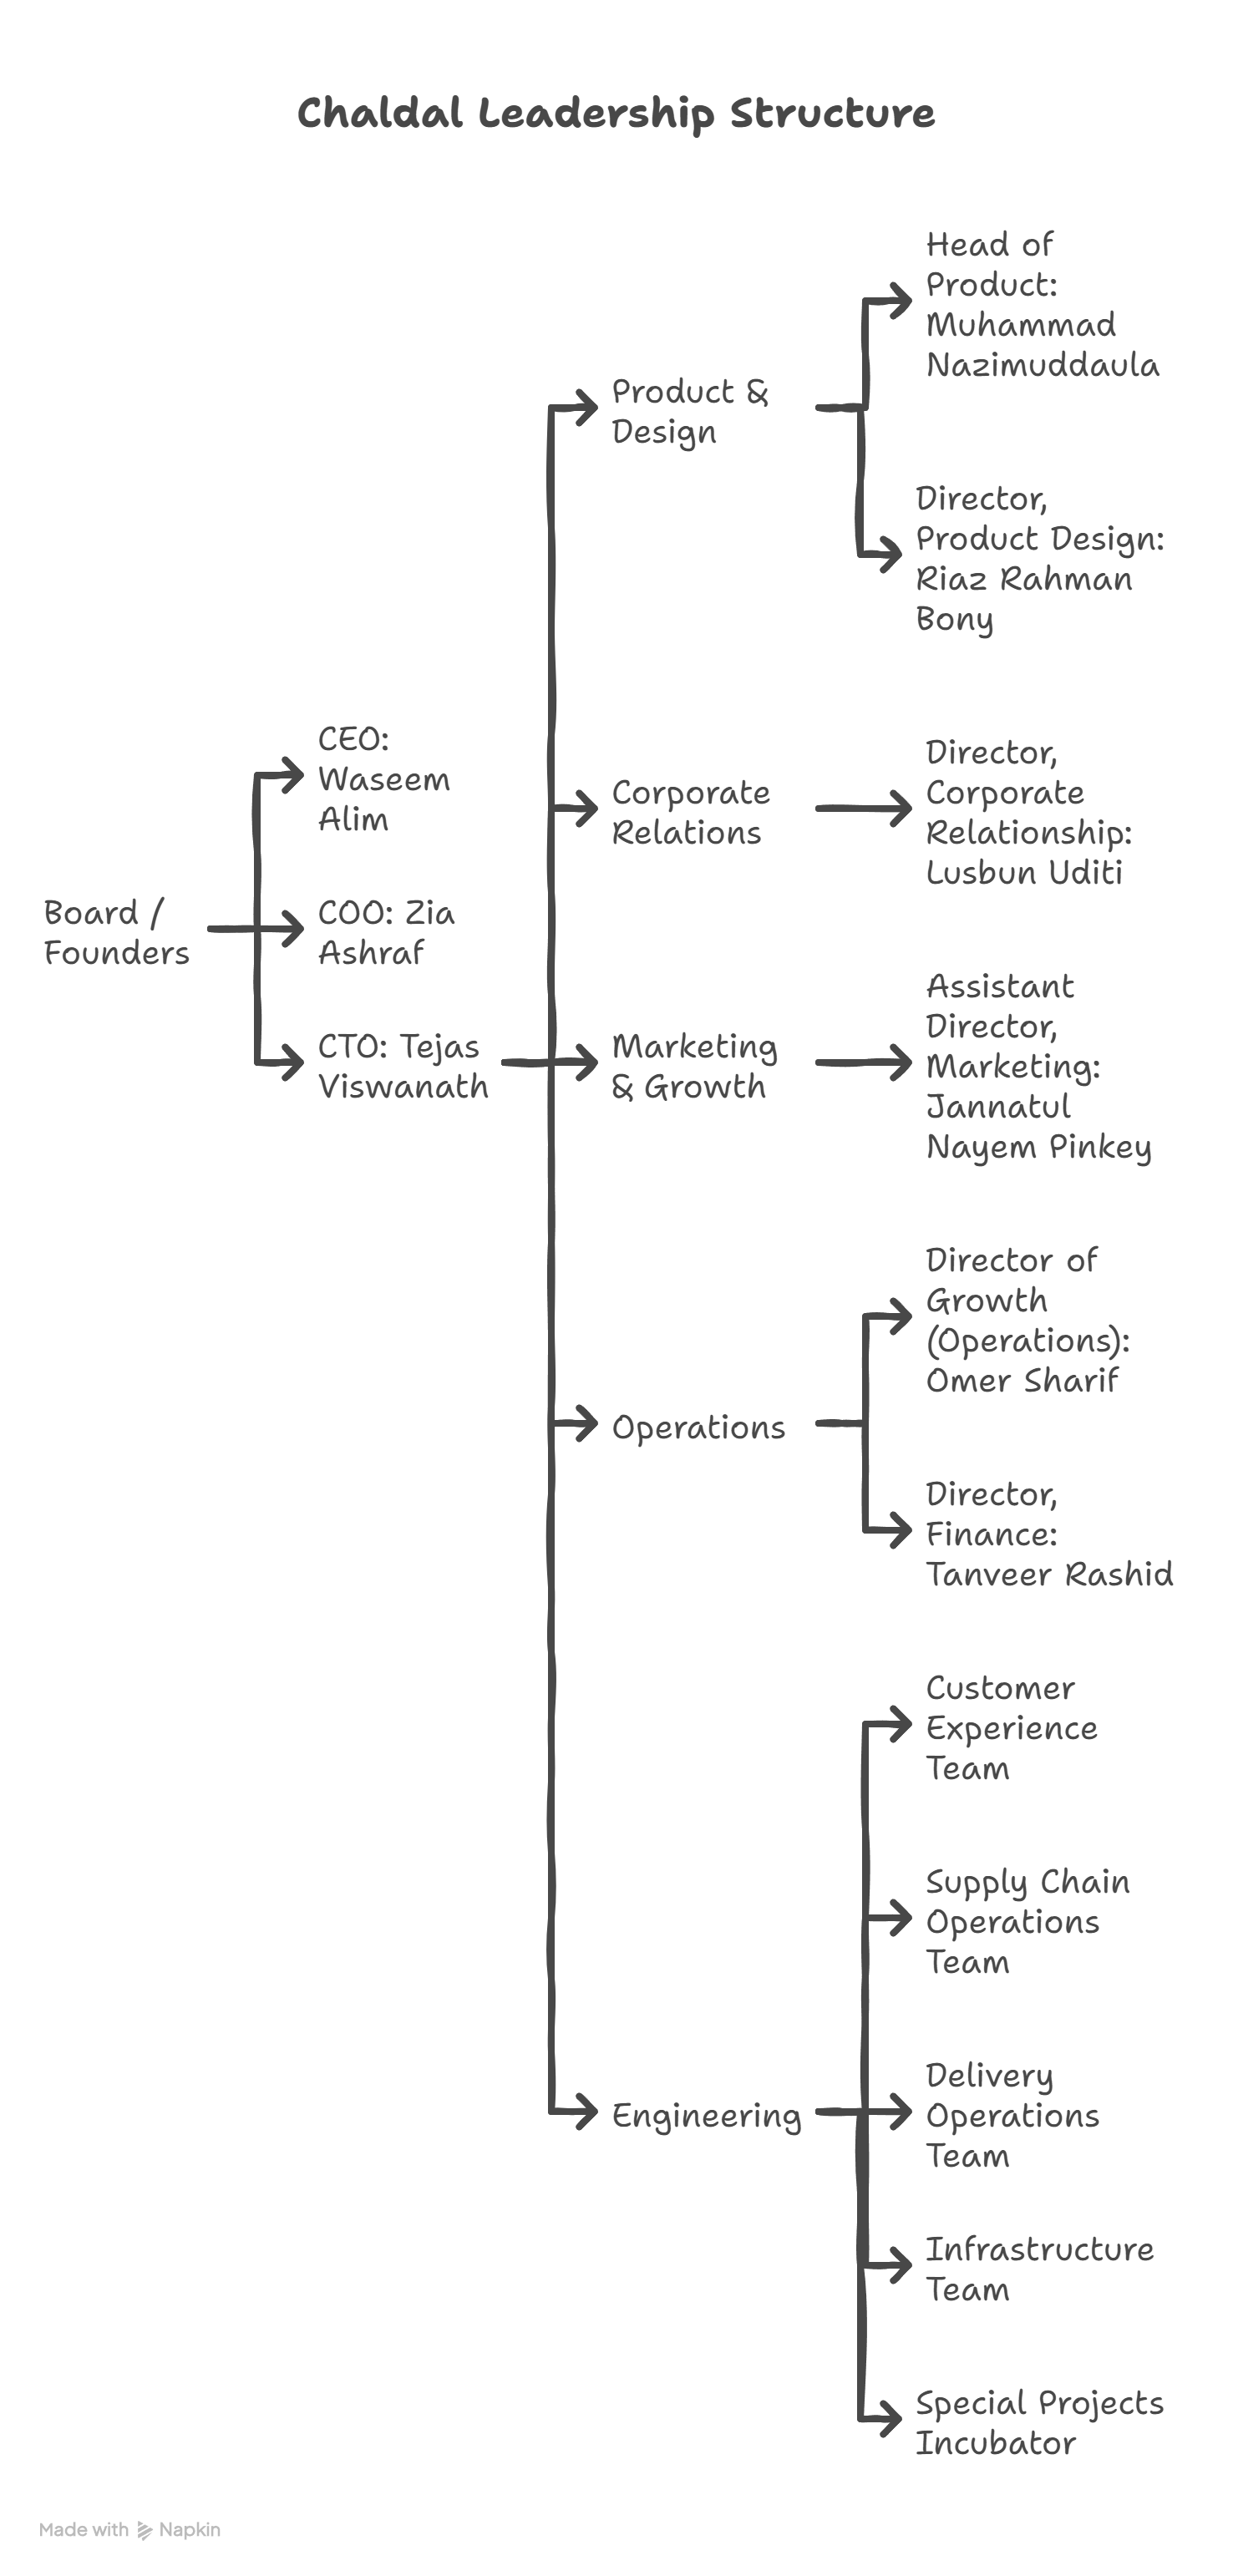
\includegraphics[width=0.7\textwidth]{Leadership Structure.png}
    % \caption{Chaldal.com Leadership Structure}
    \label{fig:leadership-structure}
\end{figure}
The Business-to-Consumer (B2C) model is an organizational set up whereby companies are selling products and services to individual clients, and not to businesses. The end-users of this model are consumers and it is all about providing them a smooth, user-friendly process in the whole range of product selection and after-sales service. Digital means of B2C businesses, including websites and mobile apps, are usually used to reach the audience broadly, support convenient transactions, and provide personalized services. The major components associated with the B2C model consists of expanding product range, direct customer contact, effective distribution systems that attempts to maximize customer satisfaction and customer loyalty.

Chaldal.com follows the B2C model, which delivers groceries and other household products sent to consumers through its online storefront. The business has a digital face that enables an individual customer to scan products, order and get the wares delivered to their doorstep. Chaldal.com minimizes the customer experience by concentrating on basic navigation, safe and secure payment methods, and ready customer care.
\begin{figure}[H]
    \centering
    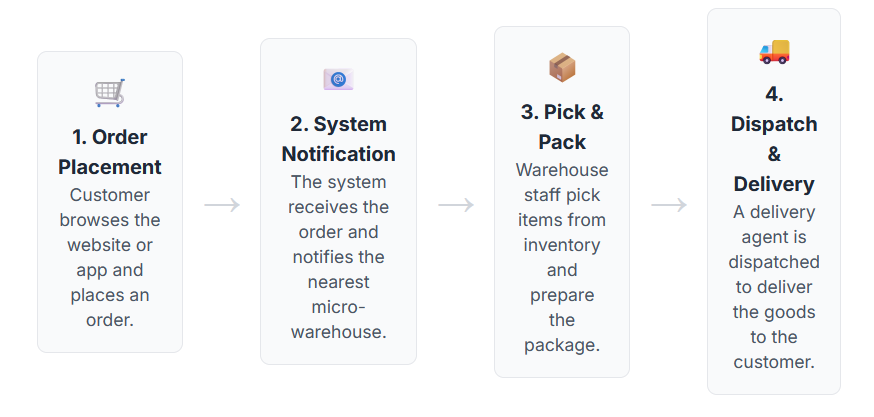
\includegraphics[width=1.0\textwidth]{b2b.png}
    \caption{B2C Model Overview of Chaldal}
    \label{fig:b2c-model}
\end{figure}
Chaldal.com collaborates with various vendors and suppliers so as to sustain a high level of items in its catalogue and to charge reasonable rates. The platform has various sources of procuring their products and keeps the inventory centralized and ensures stringent quality standards before releasing the products on to the customers. As a mediator between a number of different vendors and the final customers, Chaldal.com operates as a company which will increase the assortment of its products as well as guarantee the efficiency and reliability of the processes between the order and the final receipt of the goods.

Through its B2C approach, Chaldal.com seamlessly combines vendor collaboration, efficient inventory management, and direct-to-consumer sales to establish a robust and customer-focused online grocery service in Bangladesh.

The core of the business of Chaldal lies in a layered-logistics setup which runs through its own bespoke software systems. The company is running a micro-warehouse net in Dhaka, Chattogram, Jashore on a strategic location. These centers in location enable the firm to have in stock high demand goods near end-users and being able to deliver said ordered goods at a short time. Centralized-managed ordering combined with real-time routing algorithms enables a fleet of trained delivery people to deliver to the last mile with great accuracy in some of the most congested traffic areas of the world.

An analysis of the user age demographics reveals that Chaldal's system primarily serves a digitally native and urban-centric population. The 25-34 age group constitutes the largest segment of users at 41\%, with the adjacent 18-24 and 35-44 age groups also representing significant portions of the customer base. This concentration indicates that the core users are likely young professionals and families who are adept at using mobile technology and value the time-saving convenience offered by online grocery delivery. For the Chaldal system, this data underscores the importance of maintaining a modern, intuitive, and high-performance mobile application, as this demographic has high expectations for digital services and user experience.
\begin{figure}[H]
    \centering
    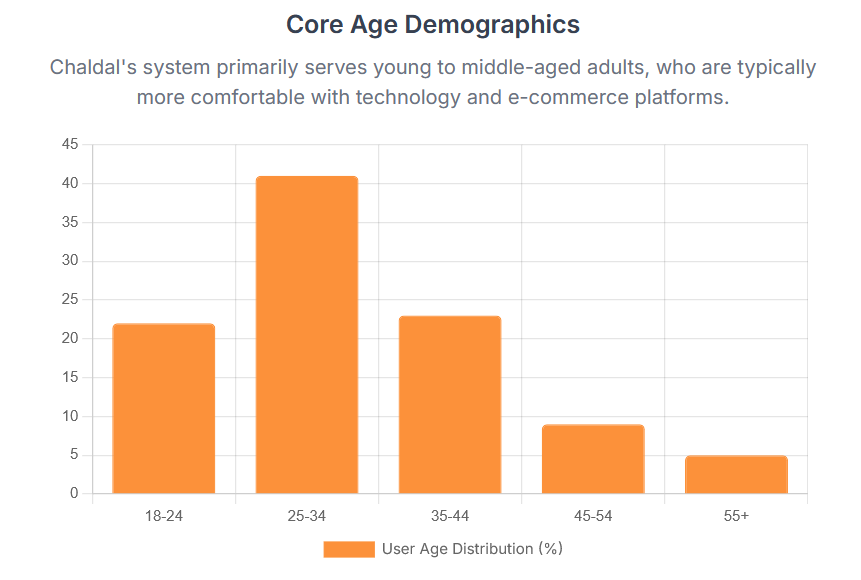
\includegraphics[width=0.8\textwidth]{user.png}
    % \caption{User age demographics Chaldal}
    \label{fig:user age}
\end{figure}
The system operated by Chaldal is rather wide-covering since it services urban households, and has corporate clients, or even international bodies like the UN World Food Programme. It can deliver tens of thousands of items orders to customers daily, groceries, household essentials, items in the pharmacy, fresh produce, meat and fish, and even ready to cook packs. The company also introduced the additional verticals, namely BanglaMeds (online pharmacy), GoGo Bangla (third-party logistics) and the Chaldal Vegetable Network (3X-farmers working directly with cities).
% \clearpage
Chaldal would have a number of closely coupled subsystems according to system engineering approach:

\textbf{Fulfillment \& Inventory Subsystem:} A distributed network of micro-warehouses, real-time stock tracking tools, and demand forecasting engines to ensure product availability and freshness.

\textbf{Technology \& Platform Management:} A proprietary software ecosystem that manages everything from inventory management to order assignment, delivery routing, customer communications, and performance analytics.

\textbf{Logistics \& Last-Mile Delivery:} A smart fleet dispatch system, trained drivers, and route-optimization algorithms that enable fast and accurate delivery within constrained time windows.
\begin{figure}[H]
    \centering
    \includegraphics[width=0.9\textwidth]{delivery Growth.png}
    % \caption{Chaldal Delivery Growth Over Time}
    \label{fig:delivery-growth}
\end{figure}
\textbf{Customer Support \& Engagement:} A responsive service team supported by CRM systems to handle order issues, feedback, and delivery updates, ensuring a consistent user experience.

\textbf{Supplier \& Farmer Network Integration:} Chaldal works directly with producers and suppliers through its own procurement system, minimizing middlemen and ensuring higher margins and fresher produce.

Chaldal leaders, led by the CEO Waseem Alim, are internationally-experienced technology, logistics and financial professionals. The experience of the founders of Silicon Valley technology, Bangladesh operations, and global systems perspective has allowed the company to develop and expand a system that is locally constrained and globally sophisticated. Heads of infrastructure, night operations, engineering, product, training, and customer experience are functional to take care of the fact that every component of the system works in harmony with other functional areas.

The systemic effect of Chaldal is tremendous. Not only does it have the distinction of introducing one-hour grocery delivery in South Asia but also has proved that micro-fulfillment can be localized even in developing economies. The COVID-19 crisis has positively impacted Chaldal as it helped the company stay relevant as a crisis utility by providing thousands of households with food. The fact that it is merged with international aid programs, the need to minimize wastage in the supply chain, and ventures into adjacent verticals demonstrate its flexibility and systemic strength.

% To sum it up, Chaldal is much more than an online grocer store--as a digital-logistics platform, it uses innovation, infrastructure and ingenuity to enable a solution to Bangladesh food distribution in the real world. Its capacity to coordinate the speedy delivery, the optimization of the chain supply as well as the expansion efficiently in cities, shows its usefulness as an infrastructure facilitator countrywide. Chaldal with its high-coordinated network of micro-warehouses, real-time technology platforms, and the last-mile logistics is an example of how one goes about creating a responsive, intelligent, mission-critical consumer supply system in the digital world.



\subsection{Problem Identification}

\begin{enumerate}
    \item \textbf{Lack of Profitability and Funding Constraints}

    Chaldal is experiencing great difficulty trying to attain sustainable profitability and ensure that it obtains sufficient finances to sustain it going forward. Constant shortage of finances does not only hinder the expansion of its operations out of Dhaka but also further restricts its branding to capital, therefore, creating a poor visibility and market penetration in other parts of the country. Such financial limitations have negative impacts on the fundamentals of business including proper maintenance of a wide product line, proper marketing campaigns, and timely paying of employees salaries. Therefore, Chaldal may find it hard to acquire new customers, maintain talented staff and match the competition in the domestic market. When left without addressed, the issues cause an imminent danger to the scalability, competitiveness, and sustainability of the company.
   
    \item \textbf{Supply Chain Inefficiencies and Product Sourcing Challenges}

    Key supply-chain inefficiencies that Chaldal still experiences include difficulty finding quality vendors and being able to procure quality goods on a regular basis, especially in the perishable and fresh produce attractor. The small suppliers base and disjointed chains of supply, together with poor inventory control frequently cause shortages, delivery problems and fluctuations in the products. Farm sourcing or local market sourcing may be too expensive and most often using the Wholesale suppliers may lead to interruptions in supplies or price wars. These difficulties not only raise the costs of purchasing, but they also undermine the reliability of the supply chains, impede the performance of the organizations with respect to providing a stable product range, and also seriously decrease the amount of customer satisfaction as well as loyalty. At the end of the day, these inefficiencies impair the profitability of the given operation and hamper the scalability of the platform.

    
    \item \textbf{Ineffective Customer Representative Operations}

    The company does not have enough budget to employ the number of full-time delivery representatives and mostly focuses on using part-time workers. This is a source of delay of the services, bad customer experience and high staff turnover. In addition, there is abuse of payment such as cash-on-delivery of some delivery workers which created a financial risk and inefficiencies in operations.
\begin{figure}[H]
    \centering
    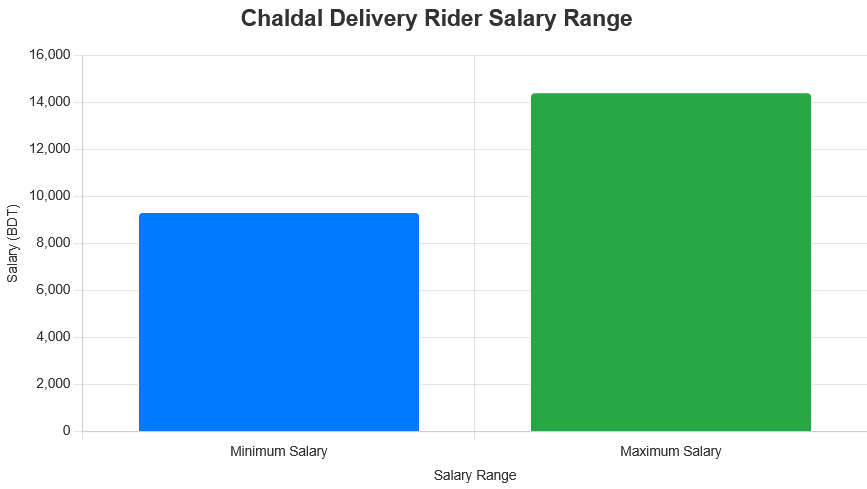
\includegraphics[width=0.9\textwidth]{salary.png}
    % \caption{Customer Representatives}
    \label{fig:Customer Representatives salary}
\end{figure}

    
    \item \textbf{Operational and HR Process Inefficiencies}

    HR, and operational routines are yet set manually such as shift scheduling and leave scheduling. This wastes superfluous administrative time and results in either or both errors in decision making or favoritism. The digital workforce management system may enhance greatly the transparency, efficiency, and scalability of the human resource operations.
    
    
    \item \textbf{Under-Optimized Application and Over-Engineered IT Infrastructure}

    The mobile app of Chaldal has a drastic performance problem, with a poor animation performance and the overall experience of the user. The areas of technical weaknesses have a direct effect on customer satisfaction and retention. Added to this are a massive skew in the engineering resource allocation side, given that the given company is processing a very small order volume of 1000-3000 orders per second on only four servers, yet it has a large engineering resource base of 35 members. Moreover, the IT infrastructure of Chaldal is over-engineered, there are several servers, and they developed their own proprietary framework. Although such systems indicate a great deal of technical ambition, they have ended up not providing such an equivalent business value. As the amount of money used in infrastructure every year surpasses 250 crore BDT, there is a question mark regarding the financial efficiency of the expenditure and sustainability of such an expenditure. Such discrepancy between engineering activities, system complexity, and business results deserves a strategic revision of application performance as well as IT resource management.
\begin{figure}[H]
    \centering
    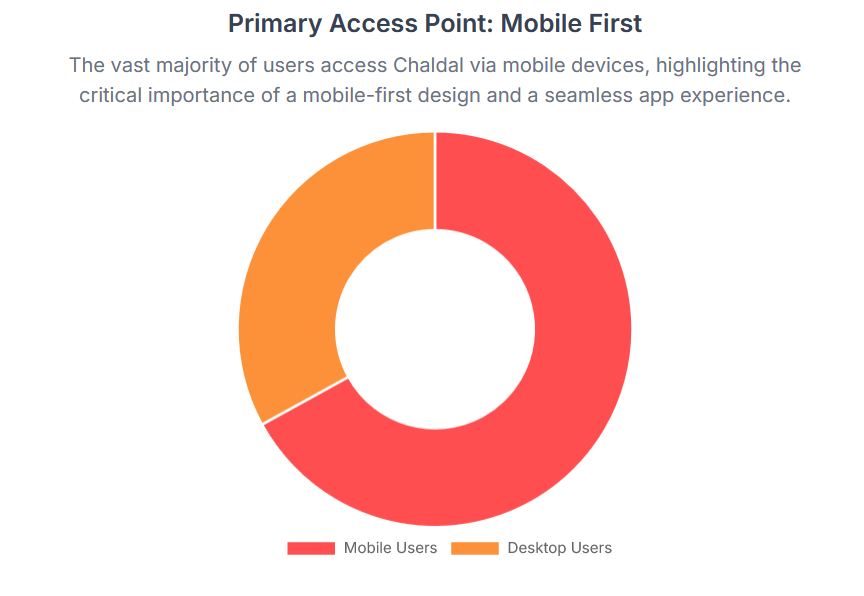
\includegraphics[width=0.9\textwidth]{device.png}
    % \caption{Primary Access point of Chaldal}
    \label{fig:device usage}
\end{figure}
\end{enumerate}

\subsection{Conclusion}

Chaldal is one of the many-layered systems that become the integration of digital commerce, urban logistics, and technological innovation. With this system analysis, we have discussed the capabilities of Chaldal as the complete fulfillment and supply chain ecosystem, which is able to service the urban consumers with speed, accuracy, and convenience, not just an e-commerce platform. Although the system has tremendous progress and radically transformed how groceries were accomplished in Bangladesh, it has encountered various vital problems that are jeopardizing its efficiency in terms of operations and its sustainability over a long period.

The analysis has revealed a number of structural and functional problems the major among which is financial instability restricting the expansion of the company geographically, investing into branding, or paying employees on a regular basis. Reservation in supply chain and unrecolored product sourcing enlightenment still impacts on customer darkens and service quality. Also, delivery functions are characterized by poor staffing, low levels of performance and manual HR terminologies, which affects the proper workforce planning. Technically, optimisation of applications is still underway and engineering resources seem to have grown too big given the output achieved, meaning that they are not aligned in terms of complexity and scale of operations.

These issues are not standalone as they are intertwined with the rest of the ecosystem of Chaldal. Finances affect recruiting, development of applications, and logistics availability. Having inconsistencies in the supply chain can influence the customer experience, revenue and the dependability of delivery. Underutilized work force and technological over engineering impose a series of inefficiencies throughout subsystems.

The challenges should be met with even-handed solution involving strategic restructuring, optimization of technology and modernization of human resources. Wholesome changes in the system-level operations, like introducing digitized HR systems, diversification of vendors, slimmer engineering policies, and performance-optimized applications can help a lot to optimize efficiency and scalability of Chaldal. Moreover, a proper balance between the operational investments and profitability targets will be necessary to make sure that the company remains relevant in the realm of a growing competitive syndicate of digital commerce.


In brief, the given system analysis identifies not only the gaps in the work operations of the Chaldal company but also precondition the interventions the company can use to address them, building a foundation to enhance its infrastructure, customer satisfaction, and long-term vision of becoming a national leader in e-grocery delivery services.



\clearpage

{\Large\bfseries\color{RoyalBlue}Chapter 2}
\vspace{0.8em}
\section{Initial Feasibility Study}
\vspace{0.6em}
\subsection{Introduction}

The first feasibility analysis will explore several operation and corporate dilemmas that block the success of Chaldal systems. Underlying both interviews with internal stakeholders and external market trends in e-grocery and tech startup sector, this chapter provides the detailed analysis of pivotal issues that impact the performance and scale-up readiness. All issues are examined in a logical manner and specific solutions are offered with the objectives of modifying them and making wise decisions.

\subsection{Initial Feasibility Analysis}
Chaldal also has a strong technical base that is comprised of: a home grown software platform, a team of engineers and micro-warehouses at locations across the city. Nevertheless, several fundamental inefficiencies exist, especially in the mobile application, which is not responsive enough and interactive. Also, the amount of engineering resources seems to be out of proportion with the system needs, which denotes the lack of proportionality in the distribution of the technical workforce. The organization is financially strained, its profitability is not achieved, and investor capital is getting scarce. There are very high operational expenses that are incurred, particularly in the logistics, infrastructure and backend maintenance without equivalent returns. This pressure is also increased by manual HR, inconsistent performance of delivery and their inability to find reliable sources of their products that slow down the workflow process. Compliance-wise, Chaldal has to work in four regulatory zones: grocery retail, pharmaceuticals, logistics, and fintech, and each of them has its own regulatory environment. As far as the existing operations are concerned, they do not seem to be out of legal boundaries, but any growth in the realm of sensitive spheres will require a heavier legality regulation. It is within this consideration of such technical, financial, operational, and legal factors that any update in the system would have to be done in phases. Short term gains like introduction of HR automation and optimization of the mobile apps would have a completion window of three to six months whereas lifting the scalability of infrastructure, financial restructuring, and comprehensive changes throughout the organization might approach long term roadmap of as much as a year and a half. The key to successful steerage through these improvements will rest on strict prioritizations, resource planning and the dynamic responsiveness against the internal and external limitations.
\subsubsection{Problem 01: Lack of Profitability and Funding Constraints}

\paragraph{Statement of the Problem}

Chaldal is not a profitable business at the present moment and continuous struggle to raise the capital needed to facilitate this sustainable growth. This has hampered its core operations in terms of product sourcing, payment of staff, territorial growth and branding. Such constraints pose a long-term threat to the business and limit its capabilities to compete on its wide market.

\paragraph{Summary of Findings}

Financial limitations of the company are very profound and complex. Underfunding has been leading to various effects including a small scale outside Dhaka to the late payment of staff salaries and slow pace of marketing to every functional unit. Internally, employees have complained of low morale because of a delayed payment of salaries as well as a failure to introduce new products. On the outside, investor sentiment fell after it was revealed that global startup funding has shrunk and Chaldal is still in high burn. There have been remarkable growth in revenue and good infrastructures but due to the inabilities to make profits, this has deterred more investments and expansion remains stagnant.

Recent reports show that Chaldal was forced to shelve its expanding initiative to cover several other cities and is currently working with a different outlook reducing loss. In 2021, it received a Series C round of about \$17 million, but further fundraising attempts since then have failed, as the world has tightened down, and investors have become more cautious. Furthermore, current marketing activities are still focused in Dhaka; they do not create brand presence in the new regional markets.

\begin{figure}[H]
    \centering
    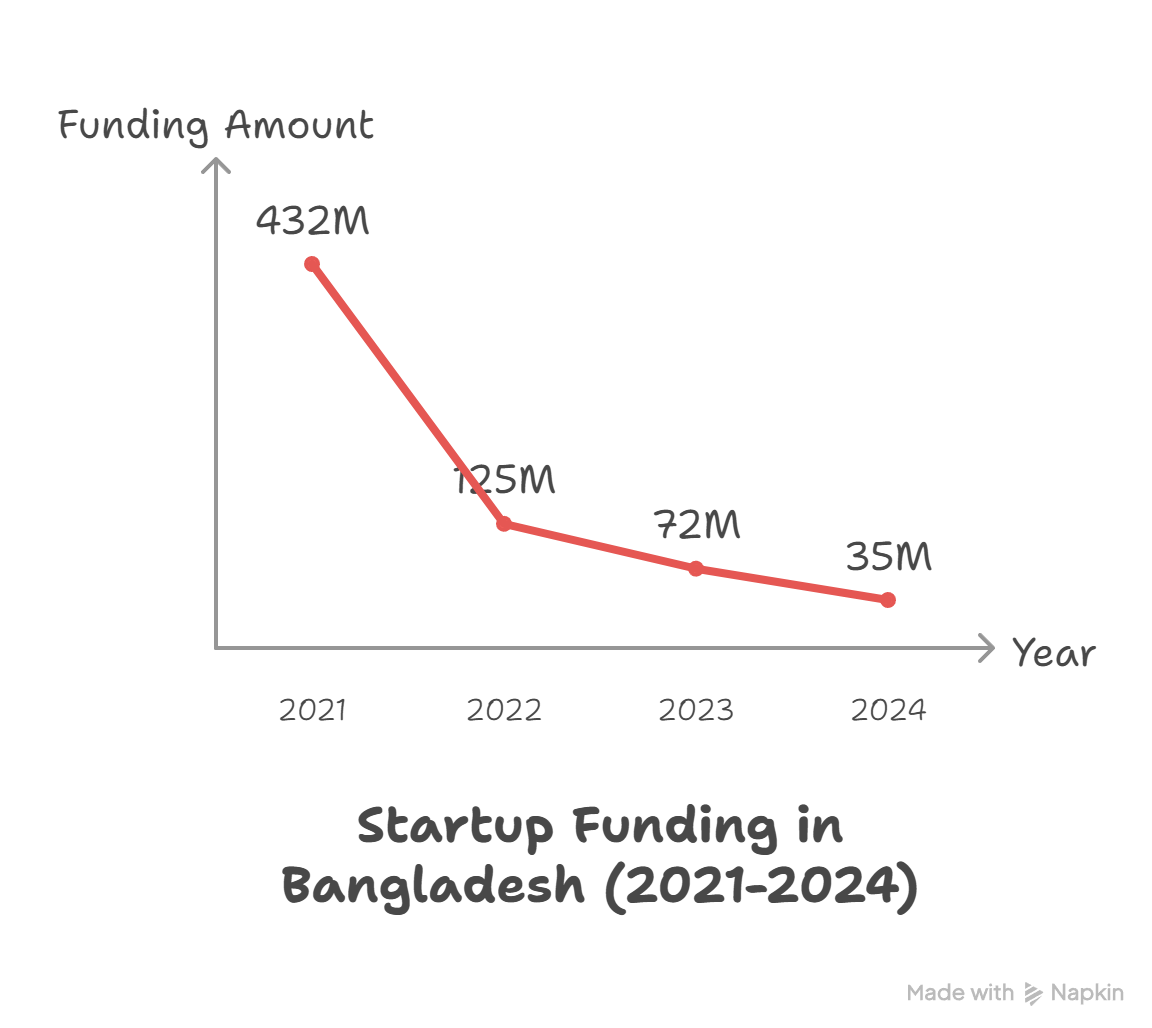
\includegraphics[width=0.7\textwidth]{Chaldal's Funding and Operational Scale graph.png}
    % \caption{Startup Funding Trends in Bangladesh (2021–2024)}
    \label{fig:startup-funding}
\end{figure}

\paragraph{Details of Findings}

\begin{enumerate}
    \item \textbf{Funding Pullback and Expansion Retrenchment}
    
    Following its opening of hubs in cities such as Jashore and Chattogram, Chaldal had to reverse the expansion because of failure to raise extra funds. Such maneuvers have seen the company get stuck in a crowded Dhaka market and has not been able to diversify its revenues.
    
    \item \textbf{Cash Flow and Salary Disbursement Issues}
    
    It was noted that not all employees, which includes the delivery representatives, receive salaries on a timely and regular basis which reduces motivation and retention. Delivery agents in other instances also mismanage cash-on-delivery collections and this introduces another cost of financial risk and loss.
    
    \item \textbf{Branding and Market Reach Limitations}
    
    The branding strategy implemented by Chaldal at the moment is largely focused on Dhaka and hardly seen elsewhere. This limits the customer intake besides increasing the difficulty of justifying into new markets growth. The corporation has no money to run a long-running digital and regional advertising market.
    
    \item \textbf{High Operating Costs vs. Revenue Output}
    
    Despite the high volume of orders, the cost per delivery is high because of the expenses in infrastructure (micro-warehouses, cold-chain logistics), employee expenses, and Technology costs. As an illustration, in spite of operating a logistics system based on four servers and own framework, the company carries out 1000 3000 orders daily, which shows that the ratio of the investment to performance is not balanced.
    
    \item \textbf{Investor Sentiment and Market Conditions}
    
    The investment in Bangladesh startup at the world level fell by 91\%, with \$432M in 2021 and 2023 only counting \$72M. With venture capital increasingly chasing profitability-first models rather than a growth-at-any-cost strategy, there are fewer reasons why a potential investor should want to invest in a venture such as Chaldal, which has no visible profit margins or unit economics that could support sustainable growth.
    
    \item \textbf{Operational Cost Overengineering}
    
    Having such in-house capacity as a larger than 35+ engineering shop and a characterized infrastructure infrastructure system are expensive overheads without commensurate returns on such costs. The system has turned out to be technically powerful but financially straining.
\end{enumerate}

\paragraph{Recommendation}

To address the profitability and funding challenges, Chaldal should adopt a profitability-first strategy that balances operational efficiency with sustainable growth. Below are specific recommendations:

\begin{enumerate}
    \item \textbf{Financial Modeling and Investor Re-engagement}
    
    Make a comprehensive unit economics dashboard in which the order-level profitability, loss reasons, and ROI of the service segment (e.g., grocery, pharmacy, logistics) are described. Apply it to business transport to local and international investors with clear fact-based arguments which have established sustainability goals as a primary goal over expansion.
    
    \item \textbf{Regional Brand Pilot and Digital Marketing Strategy}
    
    Allocate a limited but consistent budget for brand awareness campaigns outside Dhaka—targeting areas like Narayanganj or Cumilla for pilot expansion. Leverage cost-effective digital platforms (Facebook, YouTube, localized influencers) and track marketing ROI to scale successful initiatives.
    
    \item \textbf{Product and Revenue Diversification}
    
    Increase alternative sources of revenue that include BanglaMeds (electronic pharmacy), GoGo Bangla (logistical), and fintech services. Chaldal already has a license of payment gateway-this can transform or develop to digital payment wallet or utility payment gateway to increase cash flow and cut down on using grocery margins.
    
    \item \textbf{Optimize Operational Cost}
    
        Review the size of engineering team in proportion to volume of orders being received. Consider collaborating or intensive outsourcing of low priority backend maintenance to decrease internal resources strain. Introduce more conservative budgeting on server use and technology upgrade as well.
    
    \item \textbf{Lean Geographic Expansion Strategy}
    
    Repeat and go outside Dhaka again but with a lean format: One black store, one small fleet, and a local vendor base. Make feasibility test prior to full-scale rollout. The most important areas are highly populated areas, well-penetrated by the internet, and few direct competitors.
    
    \item \textbf{Align Performance with Investor Expectations}
    
    Re-position Chaldal as a stable impact driven platform. Pay more attention to such metrics as customer retention, on-time delivery, low rates of product returns, and social value (e.g., food security operations conducted during the COVID period, direct farmer support).
\end{enumerate}

\subsubsection{Problem 02: Product Sourcing and Supply Chain Inefficiencies}

\paragraph{Statement of the Problem}

Chaldal faces inefficiencies in product sourcing and supply chain management, leading to difficulties in procuring fresh, high-quality products at scale and low cost. These issues result in stockouts, higher procurement costs, and reduced customer satisfaction. Contributing factors include a weak cold chain, dependency on mediators, and inadequate vendor performance control.


\paragraph{Summary of Findings}

The existing procurement model of Chaldal is very much reliant on local suppliers and traditional markets, most of whom cannot meet the same, or lack the capacity, reliability, and consistency to supply to high-volume demands. According to employee feedback, it is hard to find reliable vendors, particularly in fresh produce. Cold chain infrastructure shortages and the use of middlemen who tend to over charge and pay less profit combines with these issues to make them even worse.

According to the external research, this is a common problem within the e-grocery industry in Bangladesh. The most often noted problems are a lack of end-to end cold logistics, disaggregated access to farm, and no certified vendor systems. Whereas Chaldal has made some efforts to initiate a direct interface between farmers and its supplies chain such as the Chaldal Vegetable Network (CDVN), this is still in an incomplete stage and does not address systemic inefficiencies.

\begin{figure}[H]
    \centering
    \resizebox{0.7\textwidth}{!}{%
    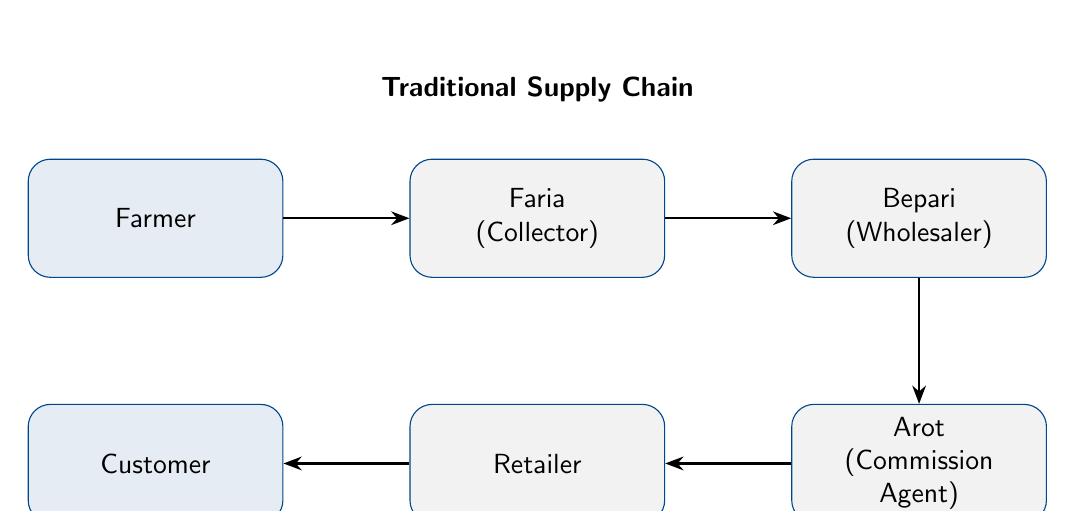
\begin{tikzpicture}[
        node distance=1.6cm and 1.6cm,
        every node/.style={font=\sffamily},
        % Increased text width and minimum height for bigger nodes
        box/.style={rectangle, draw=RoyalBlue, rounded corners=8pt, text width=3cm, align=center, minimum height=1.5cm},
        arrow/.style={thick, ->, >=Stealth}
    ]
    
    % Top row nodes
    \node[box, fill=RoyalBlue!10] (farmer) {Farmer};
    \node[box, right=of farmer, fill=gray!10] (faria) {Faria\\(Collector)};
    \node[box, right=of faria, fill=gray!10] (bepari) {Bepari\\(Wholesaler)};
    
    % Bottom row nodes (arranged right-to-left)
    \node[box, below=of bepari, fill=gray!10] (arot) {Arot\\(Commission Agent)};
    \node[box, left=of arot, fill=gray!10] (retail) {Retailer};
    \node[box, left=of retail, fill=RoyalBlue!10] (consumer) {Customer};
    
    % Arrows
    \draw[arrow] (farmer) -- (faria);
    \draw[arrow] (faria) -- (bepari);
    \draw[arrow] (bepari) -- (arot); % Arrow pointing down
    \draw[arrow] (arot) -- (retail); % Arrow pointing left
    \draw[arrow] (retail) -- (consumer); % Arrow pointing left
    
    % Label
    \node[above=0.6cm of faria] {\textbf{Traditional Supply Chain}};
    
    \end{tikzpicture}
    }
    \caption{Traditional Supply Chain Model}
    \label{fig:traditional-supply-chain-two-line}
\end{figure}

\paragraph{Details of Findings}

\begin{enumerate}
    \item \textbf{Unreliable Vendor Availability and Product Quality}
    
    According to Chaldal workers, they have found that good vendors that will be able to deliver fresh and consistent-quality goods on a large scale are hard to find. Due to seasonal trade and nonsystematic vendor activities, the products are often short in supply, returned, and cause unsatisfied customers.
    
    \item \textbf{Dependency on Middlemen}
    
    The purchasing mechanism remains rather dependent on the presence of third parties between farmers and Chaldal facilities. Such intermediaries add expenses (markups 20 to 40 percent) and allow the traceability problem. This causes the prices to be prone to fluctuations and so is the provision of quality.
    
    \item \textbf{Logistics and Cold Chain Limitations}
    
    Similar to the situation with many e-grocery services in Bangladesh, Chaldal does not have enough cold storage and refrigerated transportation opportunities. Subsequently, more of the perishable products are likely to get spoilt in the course of transportation where the ambient temperature is rampant. This not only causes wastages but also would influence the customer trust in situations where items delivered are spoilt or wilted.
    
    \item \textbf{Inaccurate Demand Forecasting and Overstocking}
    
    Although Chaldal has invested in inventory management data systems, the quick changes in demand among customers as well as the limited capacity of their warehouses are the reasons why shelves may be overstocked, or left empty of goods. When it has turnover of fresh inventory that cannot be sold on time there is direct loss of revenue when it spoils.
    
    \item \textbf{Customer Complaints and Brand Impact}
    
    Customers are also dissatisfied quite often with fruits, vegetables, and meat freshness and quality. Poor raw materials work against the credibility of a brand particularly, when it is priced expensively. These constant problems erode the competitiveness of the Chaldal among the B2C businesses in the grocery industry.
\end{enumerate}



\paragraph{Recommendation}

To fix its inefficiencies with the supply chain and sourcing, Chaldal ought to introduce a multi-faceted strategy of improvements with focus on procurement, logistics and quality of vendors:


\begin{enumerate}
    \item \textbf{Expand the Chaldal Vegetable Network (CDVN) and Establish Farmer Cooperatives}
    
    Improve the direct farmer connections that grow CDVN through major produce belts. Promote contract farming and joint participation to remove any middlemen so that prices may be better, supply less unsustainable, and traceable.

    \begin{figure}[H]
    \centering
    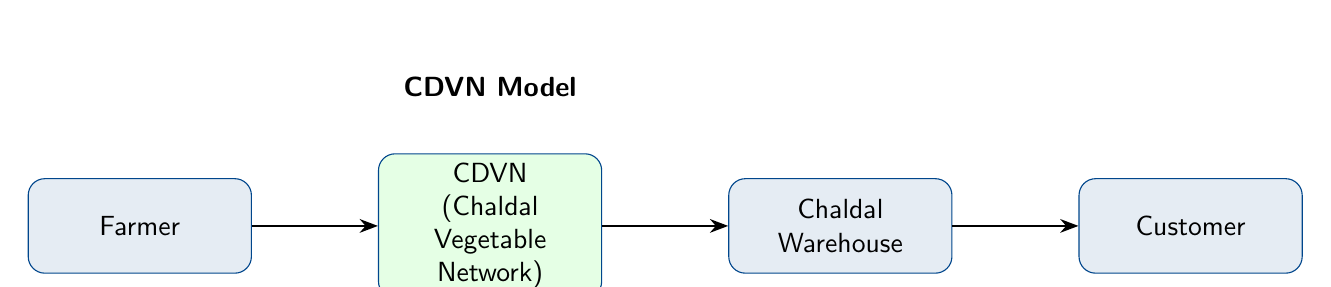
\begin{tikzpicture}[
        node distance=1.6cm and 1.6cm,
        every node/.style={font=\sffamily},
        box/.style={rectangle, draw=RoyalBlue, rounded corners=6pt, text width=2.6cm, align=center, minimum height=1.2cm},
        arrow/.style={thick, ->, >=Stealth}
    ]
    % Nodes
    \node[box, fill=RoyalBlue!10] (farmer) {Farmer};
    \node[box, right=of farmer, fill=green!10] (cdvn) {CDVN\\(Chaldal Vegetable Network)};
    \node[box, right=of cdvn, fill=RoyalBlue!10] (warehouse) {Chaldal\\Warehouse};
    \node[box, right=of warehouse, fill=RoyalBlue!10] (consumer) {Customer};
    
    % Arrows
    \draw[arrow] (farmer) -- (cdvn);
    \draw[arrow] (cdvn) -- (warehouse);
    \draw[arrow] (warehouse) -- (consumer);
    
    % Label
    \node[above=0.6cm of cdvn] {\textbf{CDVN Model}};
    \end{tikzpicture}
    \caption{Chaldal Vegetable Network (CDVN) Model}
    \label{fig:cdvn-model}
\end{figure}
    % \clearpage
    \item \textbf{Invest in Cold Chain Logistics and Regional Warehouses}
    
    Establish or engage in collaborations with cold storage services to establish an efficient cold chain on the perishable items. Provide temperature-controlled micro-warehouses in the hot market locations. Use development grants or impact funding (e.g. IFC, ADB) to fund energy and infrastructure improvements.
    
    \item \textbf{Implement a Certified Vendor Program}
    
    Build a model of vendor certification that is carried out through periodic audits, testing of the goods, timely shipment, and packaging regulations. High-performing vendors may be preferred in procurement pipelines and rewarded by bulk contracts or by performance bonuses.
    
    \item \textbf{Enhance Demand Forecasting through AI and Real-Time Analytics}
    
    Improve inventory planning using predictive algorithms that analyze real-time sales, seasonal trends, and historical data. Automate purchase order generation to prevent overbuying and spoilage. Integrate warehouse dashboards that sync stock levels with frontend availability to prevent customer order failure.
    
    \item \textbf{Introduce Price Transparency and Shelf-Life Based Discounts}
    
    Instill a feeling of consumer confidence in transit of details on sourcing and dynamic pricing models. Sell close to expiration or otherwise marred-but-still-edible produce at a discount in real-time in order to minimize it. This also assists in the creation of an image of values in the price conscious market.

\end{enumerate}

Chaldal can help save a lot of wastage, make the quality of the product much better and increase customer satisfaction by improving vendor networks, modernizing logistics and gaining a smarter procurement using technology. The direct outcome of these improvements will be an increase in margins and contribute to the journey towards the profits of Chaldal.

\subsubsection{Problem 03: Ineffective Customer Representative \& Delivery Operations}

\paragraph{Statement of the Problem}

Chaldal’s reliance on undertrained and underpaid part-time delivery staff results in inconsistent service quality, increased theft or fraud, and customer dissatisfaction. These issues are worsened by an inadequate software-based agent selection system and the financial risks tied to cash-on-delivery payments.
% \clearpage

\paragraph{Summary of Findings}

\begin{itemize}
    \item \textbf{Staff shortages \& bad incentives:} Lack of stable, full-time delivery staff leads to irregular attendance, low accountability, and poor service.
    \item \textbf{Cash-on-delivery vulnerabilities:} COD increases the risk of fraud, erratic cash handling, and cash flow delays—echoing national trends where COD still dominates but remains risky.
    \item \textbf{Lack of delivery oversight \& training:} Reports from similar platforms highlight delayed deliveries and poor rider behavior as key pain points.
    \item \textbf{Geography-based operational gaps:} Automated agent assignments without location optimization can increase delivery times and route inefficiencies.
\end{itemize}

\paragraph{Details of Findings}

\begin{enumerate}
    \item \textbf{Understaffing and Part-Time Reliance}
    
    Employees observe that Chaldal can not hire a sufficient number of full time deliveries due to the lack of funds. Part-time riders are infrequently motivated, behave intermittently, have unstable finances, and a tendency of being retentive.
    
    \item \textbf{Cash-on-Delivery Risk Exposure}
    
    According to national reports, 75\% of e-commerce payments in Bangladesh represent COD and this not only encourages fraud but also delays in the settlement of funds and as banks payout only after confirmation, which will make cASH flow of Chaldal difficult to manage.
    \begin{figure}[H]
        \centering
        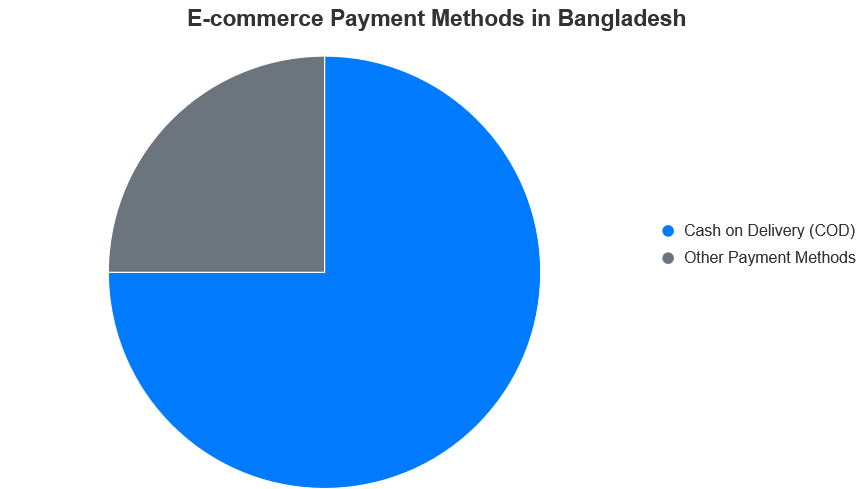
\includegraphics[width=0.7\textwidth]{cash on delivery.png}
        % \caption{Cash-on-Delivery Process and Risks}
        \label{fig:cash-on-delivery}
    \end{figure}
    
    \item \textbf{Customer Complaints About Service Quality}
    
    As it is observed throughout e-commerce, late delivery, inefficient packaging, unprofessional conduct of riders, and such a problem as a lack of hygiene control are common issues. Chaldal drivers have the potential to reproduce such bad stories without having any formal demands and orders established.
    
    \item \textbf{Absence of Efficient Selection and Assignment Software}
    
    Employees pointed to the flaws of Chaldal current agent-selection system that in many cases assigns riders to unoptimal factors instead of proximity or previous performance, leading to slower order delivery and inefficient use of resources.
    
    \item \textbf{Safety and Worker Welfare Gaps}
    
    Similarly to the case of food delivery workers, Chaldal riders work in environments to which they are not properly trained and on which they have no benefits with regard to health and safety. Industry criticisms would require an improvement of insurance, safe transportation paraphernalia, and rider encouragement to maintain morale and performance.
\end{enumerate}

\paragraph{Recommendation}

In order to enhance the delivery process and restore customer confidence, Chaldal ought to do the following:

\begin{enumerate}
    \item \textbf{Shift Toward Stable, Full-Time Riders with Proper Compensation}
    
    Replace a mainly part-time system with full-time employees in the staffs essential shifts. Pay good salaries, performance bonuses, and retained compensation to enhance controllability and eliminated lapses in the services.
    
    \item \textbf{Introduce Cashless and Prepaid Payment Options}
    
    Speed up the hardware taking on-line payments (bKash, Nagad, UPAY) by rewarding prepaid orders-giving discounts or points on made without COD (descended). This reduces cash management risks and enhances the cash flow.
    
    \item \textbf{Deploy Rider Training \& Accountability Framework}
    
    Conduct compulsory hygiene, customer services training, safety, and payment training. Devise measures e.g. punctuality in delivering, customer rating and incidents and have them related to reviews, incentivization or disqualification.
    
    \item \textbf{Implement Smart Agent-Assignment Software}
    
    Decide and incorporate geo-based routing software to assign available riders depending on the proximity, the capacity to carry, and previous performance. This maximizes the time of delivery and balances of loading in each neighborhood.
    
    \item \textbf{Enhance Worker Welfare and Support Systems}
    
    Collaborate with insurance providers to provide simple accident and health cover to riders. Equip them with security equipment (helmets, vests), enact mechanisms through which riders may bring grievances on you- developing a respectful and sustainably-growing workforce.
\end{enumerate}

Chaldal can provide the delivery team with a professional approach, promoting cashless purchases, and invest in intelligent dispatch systems to radically increase the level of reliability, reduce delivery time, and improve consumer satisfaction to turn delivery services into the service advantage.

\subsubsection{Problem 04: Operational and HR Process Inefficiencies}

\paragraph{Statement of the Problem}

The HR and operational functions of Chaldal including shift planning and leave management are still being done manually. It results in inefficiency in administration, mistakes and possible favorism which would have a detrimental effect on employee morale and lack of transparency in operations.

\paragraph{Summary of Findings}

HR work that is done manually takes a considerable amount of time and makes the work susceptible to errors. Employees report discrepancies in allocating shifts and approvals of leave which in some cases, leads to conflicts or indignation of unfairness. It is also hard to trace attendance, overtime and performance indicators without a digital system making data based decisions very hard to be made.

\paragraph{Details of Findings}

\begin{enumerate}
    \item \textbf{Manual Scheduling and Leave Management}
    
    The HR personnel waste a lot of time on the routine scheduling, which is sometimes done via spreadsheets or even paper records. This multiplies the chances of being overbooked, skipping shift, or taking unauthorized leaves.
    
    \item \textbf{Lack of Transparency and Auditability}
    
    It is hard to audit HR decisions objectively and may be impossible to settle disputes without any digital trace. Employees can feel that the changes in shifts and leaves are made on a biased basis.
    
    \item \textbf{Limited Performance Tracking}
    
    This is because there is no integrated HR software and therefore no systematic collection or analysis of performance data (i.e. attendance, punctuality, overtime etc.) It is therefore hard to develop specific training or reward.
\end{enumerate}

\paragraph{Recommendation}

\begin{enumerate}
    \item \textbf{Implement a Digital Workforce Management System}
    
    Implement an HR software platform that will automate schedule creation, leave requests and attendance management. This will save administrative efforts, limit mistakes and enhance openness.
    
    \item \textbf{Standardize HR Policies and Communication}
    
    Obviously record and communicate HR policies on shifts, leaves, and performance evaluation. Make sure that these guidelines are made available to all the employees.
    
    \item \textbf{Enable Data-Driven HR Decisions}
    
    Track the trends in absenteeism, overtime, and productivity with the help of the HR system analytics. Use the data to engage in specific interventions and constant improvement.
\end{enumerate}


\subsubsection{Problem 05: Under-Optimized Application and Over-Engineered IT Infrastructure}

\paragraph{Statement of the Problem:}
Despite having a strong engineering team, Chaldal’s mobile application remains under-optimized, with slow loading times, outdated animations, and inconsistent responsiveness—negatively affecting user experience. Additionally, its large-scale engineering infrastructure appears oversized relative to platform traffic and order volume, leading to disproportionate operational costs.

\paragraph{Summary of Findings:}

There are problems related to the performance of the app (they could not eliminate lags, glitches, and the lack of animation).\\
Over-allocation of resources: There are more than 35 engineers working with a rather simple user interface and, at some point, 1000-3000 orders per day which is a sign of a poor utilization of resources.
Based on customer rating and industry standard, an effective e-commerce application is responsive, interactive in real time, and with smooth UI, which cannot be found in the application of Chaldal.
Money spent on infrastructure (custom-built framework and servers) has not been converted to improvement in terms of user growth, or performance.
The work of the developers is also shifted towards backend maintenance, whereas the frontend aimed at the user is ignored.\\


\paragraph{Details of Findings}

\begin{enumerate}
    \item \textbf{Subpar User Experience}
    
 The customers often complain about delayed service, slow navigating and obsolete design. The app is no longer than, say, an app like Daraz or Foodpanda, which focuses on micro-interaction, zippy performance, and fluid design.    
    \item \textbf{Disproportionate Engineering Resources}
    
 The firm has a seemingly scarce order throughput (which ranges between 1000-3000 orders each day), but it can employ a significant number of engineers and have several designated servers. According to internal interviews, much of the work of engineers involves infrastructure and backend systems, and not making direct user differences.    
    \item \textbf{Lack of UI/UX Optimization}
    
 The app does not include smooth transitions, dynamic filtering, responsive animations, and instant feedback buttons that are crucial in creating good user experience. It is a lost opportunity since the quality of user interface has a major influence on retention rates in mobile-first economies, e.g. Bangladesh.
     \item \textbf{Server and Framework Maintenance Costs}
    
 Chaldal operates atop of home grown software platform with four servers one of which is proprietary. Although such an infrastructure is technically impressive, it would require constant developer resources and is expensive to operate. The payback of this investment is uncertain to a company that always aims at achieving profitability.
     \item \textbf{Misaligned Development Priorities}
    
 According to interviews with industry employees and app store reviews, a large number of startups give preference to lean, iterative frontend phase using agile design sprints. Conversely, it seems Chaldal has had a dev pipeline that is significantly frontend-lacking, thus causing sluggish improvements to the frontend, and the presence of a less-than-optimal user experience.
\end{enumerate}

\paragraph{Recommendation}
In order to maximize the output of the engineering arms and the satisfaction of the end-user, Chaldal ought to pursue a two-pronged approach of improving app performance and reallocating engineering resources toward efficiency:

\begin{enumerate}
    \item \textbf{Redesign and Optimize the Frontend App}
    
Use UX audit and gradually present the enhancement: loading should be faster, better to navigate to explore the products, to do transition easier, and gestures should be natural. Focus on high-performance by using lightweight design, which will work on cheaper smartphones.    
    \item \textbf{Adopt Performance Monitoring Tools}
    
Add such tools as Firebase Performance Monitoring or Datadog to gather real-time data about app performance (e.g., time-to-interaction, how quickly any screen loads). Take advantage of these insights to make decisions about prioritizing the bug fixes and optimization.    
    \item \textbf{Restructure Engineering Priorities and Headcount}
    
     Redistribute a part of the engineering capacity on the infrastructure to frontend/mobile teams. Costs were to be managed by calculating the necessity of all backend functions or whether any maintenance can be outside or automated.
    \item \textbf{Focus on Business-Driven Technology Investments}
    
   Reflect on the fact that the proprietary servers and a custom backend framework may no longer have a competitiveAD Offer. Otherwise, port some of them to cloud-native and scalable services (e.g. AWS Lambda, Firebase) to achieve less overhead.
   \item \textbf{Implement Agile Product Development Cycles}
    
 Use bi-weekly sprints focused on small, impactful user-facing features. Involve design, QA, and product managers early in the process to ensure engineering outputs align with business and customer needs.\end{enumerate}

\subsection{Conclusion}

This assessment of the first possible feasibility of Chaldal shows that it is a very ambitious concept and is not limited now by several hard operational, financial and technical issues. As a result of systematic review analysis of interviews with the stakeholders and cross-correlated industry studies, six interdependent issues that contribute to the performance and scalability of the total organization have been illuminated in the chapter.

Top of these is the continuous challenge that the firm faces in becoming profitable and having sustainable capital. Straight down this financial strain constrains branding, scale of business in a way that only allows operation in Dhaka, and employee retention. Adding to this is an ineffective supply chain marred with unstable supply of vendors, unstable supply of products, lack of proper cold chain facilities-weakening the quality of the products and making the suppliers retrospectively more costly. Delivery operation is also undermined by lack of investments in human capital, where part-time riders bring uncertainties, risks to payments, and customer dissatisfaction.

On the inside, manual HR operations at Chaldal congest workflow and incur administrative inefficiency making the business less able to increase operations and ensure staff accountability. Through the technological axis the company has been burdened with having a disproportionately huge engineering team and having an overall over-engineered infrastructure, and the mobile application that the company provides to its consumer base is not properly optimized and is outdated. This imbalance shows that resource allocation is not in touch with business output and this is a further drag in the operations.

Nevertheless, despite these issues, the modus operandi of control, the micro-warehouse system, the vertically integrated logistics, and the data-driven system of fulfilling orders prove to have large potential that Chaldal has to offer. The problems disclosed in this chapter are the ones that belong to problematic execution and utilization of resources rather than to a problematic vision. Through careful re-organizing, specific technology investments, and a course to focus on being profitable in every venture, Chaldal can not only be able to adequately meet its existing constraints but even develop itself into a stronger position in the digital commerce paradigm in Bangladesh.
The given feasibility study prepares the base to the further work in system development. Focusing on the outlined issues and problem-solving using data and creating an enhanced governance and customer-oriented innovation, Chaldal has an opportunity to develop a stronger, more effective, and scalable system that will meet business objectives as well as stakeholder demands

\clearpage

{\Large\bfseries\color{RoyalBlue}Chapter 3}
\vspace{0.8em}
\section{Analysis}
\vspace{0.6em}

\subsection{Introduction}
% Introducing the purpose and scope of Chapter 3
The analysis phase of the Chaldal System Analysis Report serves as a critical step in dissecting the operational, financial, and technical challenges identified in Chapters 1 and 2, which impede Chaldal’s ability to achieve sustainable growth and operational efficiency in Bangladesh’s competitive e-grocery market. This chapter focuses on a detailed investigation of the five core problems outlined previously: (1) lack of profitability and funding constraints, (2) product sourcing and supply chain inefficiencies, (3) ineffective customer representative and delivery operations, (4) operational and HR process inefficiencies, and (5) under-optimized mobile application and over-engineered IT infrastructure. These issues, as established, are interlinked, with financial constraints exacerbating operational inefficiencies, supply chain limitations affecting customer satisfaction, and technical misalignments inflating costs without proportional business value. 

The objective of this chapter is to systematically gather and analyze data to validate these problems, uncover their root causes, and provide actionable insights for strategic interventions. By employing a multi-method information-gathering approach—comprising literature reviews, on-site observations, stakeholder interviews, and questionnaires—this chapter ensures a comprehensive examination of Chaldal’s ecosystem. The gathered data will be synthesized and represented through analytical tools, including charts, graphs, and diagrams, to visually articulate the extent and impact of each issue. These visual aids will facilitate a clearer understanding of the systemic challenges and guide the formulation of targeted recommendations. Ultimately, this chapter aims to bridge the gap between problem identification and solution design, positioning Chaldal to enhance its operational efficiency, customer experience, and long-term sustainability in the rapidly evolving digital commerce landscape.

% Introducing a conceptual diagram of the analysis framework
To illustrate the interconnected nature of Chaldal’s challenges, Figure \ref{fig:analysis_framework} presents a conceptual framework that maps the five problems to their respective subsystems and their impact on overall business performance. This diagram serves as a roadmap for the analysis, highlighting how each issue influences Chaldal’s operational and strategic outcomes.

By conducting thorough information gathering and detailed analysis, system analysts can
gain a deep understanding of the system’s context and stakeholders’ needs. This enables
them to make informed decisions and propose appropriate solutions that align with the
goals and requirements of the organisation or project.

\begin{figure}[H]
\centering
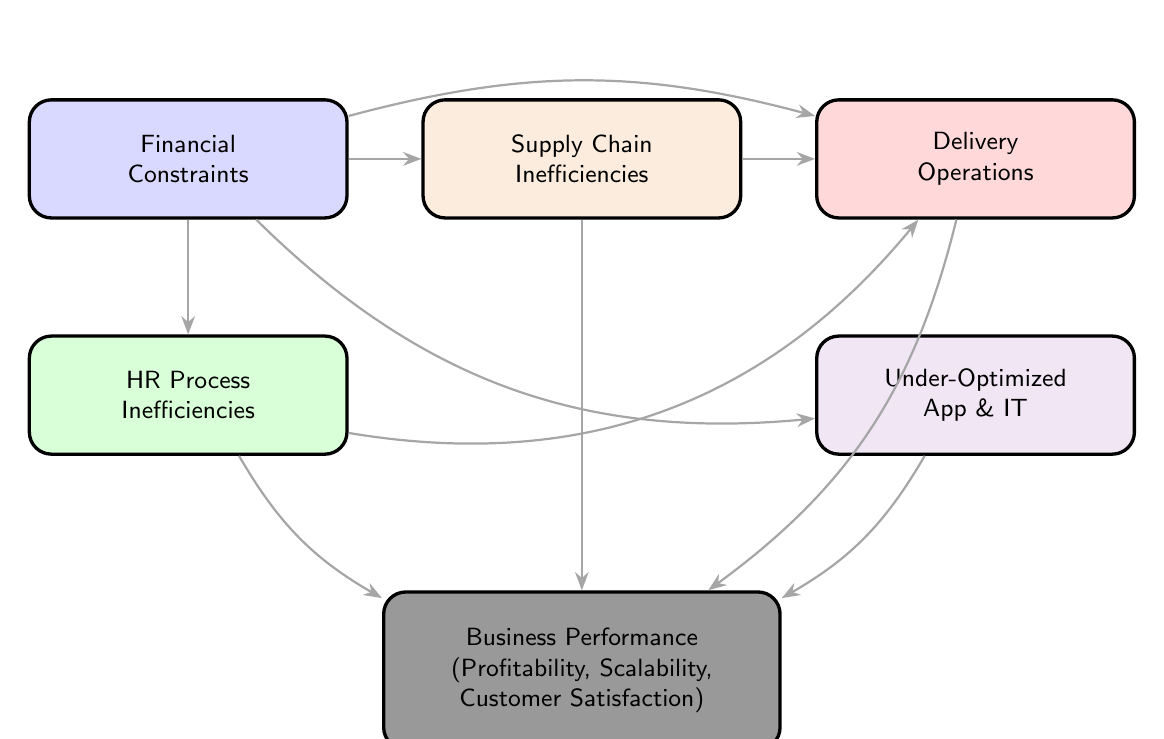
\begin{tikzpicture}[
  node distance=2.5cm and 4cm,
  box/.style={rectangle, draw=black, rounded corners=8pt, minimum height=1.5cm, minimum width=4cm, align=center, font=\small, text width=3.8cm, fill=#1!15, text=black, line width=1.2pt},
  arrow/.style={-Stealth, thick, color=gray!70}
]

% Top row nodes
\node[box=blue] (finance) at (0,3) {Financial\\Constraints};
\node[box=orange] (supply) at (5,3) {Supply Chain\\Inefficiencies};
\node[box=red] (delivery) at (10,3) {Delivery\\Operations};

% Middle row nodes
\node[box=green] (hr) at (0,0) {HR Process\\Inefficiencies};
\node[box=purple] (tech) at (10,0) {Under-Optimized\\App \& IT};

% Bottom node (centered and larger)
\node[box=gray, fill=gray!80, minimum width=5cm, minimum height=2cm, text width=4.8cm] (performance) at (5,-3.5) {Business Performance\\(Profitability, Scalability,\\Customer Satisfaction)};

% Arrows from Financial Constraints
\draw[arrow] (finance) -- (supply);
\draw[arrow] (finance) to[bend left=15] (delivery);
\draw[arrow] (finance) -- (hr);
\draw[arrow] (finance) to[bend right=25] (tech);

% Arrows from Supply Chain
\draw[arrow] (supply) -- (delivery);
\draw[arrow] (supply) -- (performance);

% Arrows from Delivery
\draw[arrow] (delivery) to[bend left=20] (performance);

% Arrows from HR
\draw[arrow] (hr) to[bend right=30] (delivery);
\draw[arrow] (hr) to[bend right=15] (performance);

% Arrows from Tech
\draw[arrow] (tech) to[bend left=15] (performance);

\end{tikzpicture}
\caption{Conceptual Framework of Chaldal's Systemic Challenges}
\label{fig:analysis_framework}
\end{figure}

\subsection{Information Gathering}
% Outlining the multi-method approach for data collection
To comprehensively analyze the five identified problems, a robust information-gathering strategy was employed, integrating four distinct methods: (1) review of literature, procedures, and forms; (2) on-site observations; (3) interviews with key stakeholders; and (4) questionnaires targeting employees, delivery personnel, and customers. Each method was tailored to address the specific challenges outlined in Chapter 2, ensuring that both qualitative and quantitative data were collected to provide a holistic view of Chaldal’s operational ecosystem. These methods were selected to capture internal operational dynamics, external market trends, and stakeholder perspectives, thereby validating the severity and interconnections of the identified issues.

% Explaining the relevance of each method
The review of literature, procedures, and forms leverages existing documentation and industry reports to contextualize Chaldal’s challenges within the broader e-commerce and logistics landscape. On-site observations provide direct insights into operational workflows, particularly in micro-warehouses and delivery processes, to identify inefficiencies firsthand. Interviews with key personnel—ranging from management to delivery riders—offer qualitative depth, uncovering root causes and operational pain points. Questionnaires, designed with diverse formats (e.g., yes/no, Likert scale, and ranking questions), target a broader audience to quantify the prevalence and impact of issues across Chaldal’s workforce and customer base. Together, these methods ensure a data-driven approach to problem validation and solution formulation.

% Introducing a diagram of the information-gathering process
Figure \ref{fig:info_gathering} illustrates the information-gathering process, showing how each method contributes to the analysis of Chaldal’s systemic challenges. This visual representation underscores the iterative and interconnected nature of the data collection, ensuring comprehensive coverage of the five problems.

\begin{figure}[H]
\centering
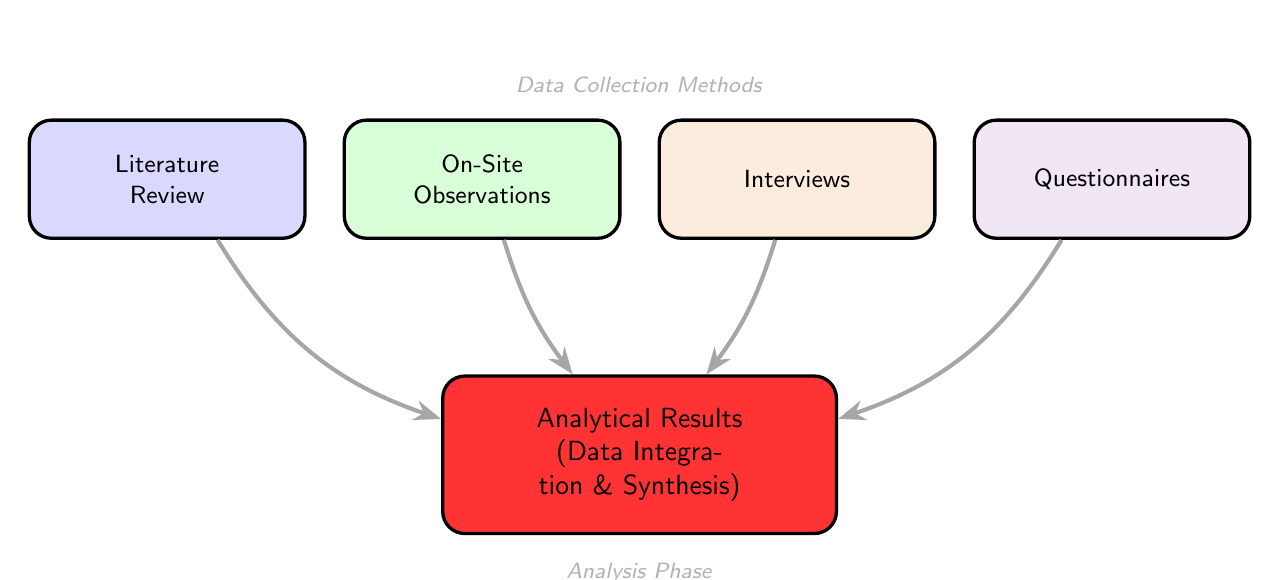
\begin{tikzpicture}[
  node distance=2cm and 3cm,
  box/.style={rectangle, draw=black, rounded corners=8pt, minimum height=1.5cm, minimum width=3.5cm, align=center, font=\small, text width=3.2cm, fill=#1!15, text=black, line width=1.2pt},
  arrow/.style={-Stealth, thick, color=gray!70, line width=1.5pt}
]

% Top row nodes - data collection methods
\node[box=blue] (lit) at (0,2) {Literature\\Review};
\node[box=green] (obs) at (4,2) {On-Site\\Observations};
\node[box=orange] (int) at (8,2) {Interviews};
\node[box=purple] (quest) at (12,2) {Questionnaires};

% Bottom node - analytical results (centered and larger)
\node[box=red, minimum width=5cm, minimum height=2cm, text width=4.5cm, font=\normalsize, fill=red!80] (analysis) at (6,-1.5) {Analytical Results\\(Data Integration \& Synthesis)};

% Arrows from all data collection methods to analytical results
\draw[arrow] (lit) to[bend right=20] (analysis);
\draw[arrow] (obs) to[bend right=10] (analysis);
\draw[arrow] (int) to[bend left=10] (analysis);
\draw[arrow] (quest) to[bend left=20] (analysis);

% Optional: Add method category labels
\node[font=\footnotesize, color=gray!60] at (6,3.2) {\textit{Data Collection Methods}};
\node[font=\footnotesize, color=gray!60] at (6,-3) {\textit{Analysis Phase}};

\end{tikzpicture}
\caption{Information-Gathering Process for Chaldal's System Analysis}
\label{fig:info_gathering}
\end{figure}


\subsubsection{Review of Literature, Procedure, and Forms}
To thoroughly understand Chaldal’s operational ecosystem and identify the systemic challenges impacting its scalability, a detailed review was conducted, encompassing secondary literature, internal operational procedures, and key forms used in daily operations. This subsection synthesizes findings from official sources, media interviews, academic case studies, and industry reports, providing a comprehensive view of Chaldal’s workflows, technological infrastructure, and operational bottlenecks.\\

\vspace{.4em}
{\large\bfseries Review of Literature}

The literature review explored Chaldal’s operational model, technological capabilities, and logistical framework, drawing from diverse sources to contextualize its performance within the e-commerce landscape of Bangladesh and beyond:
\begin{itemize}
    \item \textbf{Chaldal Official Website} (\url{https://chaldal.com}): The website offers an in-depth look at Chaldal’s service offerings, including its extensive product catalog (over 20,000 SKUs), same-day delivery commitment within 1-2 hours in urban areas, and its network of micro-warehouses strategically located across Dhaka, Chittagong, and other major cities. It highlights Chaldal’s focus on customer convenience, with a user-friendly interface and mobile app supporting both Android and iOS platforms.
    
    \item \textbf{Interviews \& Talks}: Insights from interviews with Waseem Alim, Chaldal’s Founder and CEO, published in outlets like The Daily Star and Dhaka Tribune, and on platforms like YouTube, reveal the company’s strategic vision. Alim emphasized Chaldal’s micro-warehouse model as a solution to Bangladesh’s urban density and traffic challenges, but he also noted difficulties in scaling logistics due to infrastructure limitations and high operational costs. A 2023 interview highlighted that Chaldal handles over 10,000 daily orders in Dhaka alone, underscoring the pressure on its supply chain.
    
    \item \textbf{Relevant Case Studies}: Comparative analysis with global e-commerce players like Instacart (USA), BigBasket (India), and RedMart (Singapore) provided benchmarks for operational efficiency. For instance, BigBasket’s use of AI-driven demand forecasting and automated warehousing contrasts with Chaldal’s reliance on semi-manual processes. These case studies suggest that Chaldal could benefit from adopting predictive analytics and automation to enhance scalability.
    
    \item \textbf{Industry Reports}: Reports from the Bangladesh E-commerce Association (eCAB) and global consulting firms like McKinsey indicate that Bangladesh’s e-commerce sector is projected to grow at a CAGR of 15\% through 2027, driven by increasing smartphone penetration (over 50\% of the population by 2025) and urban consumer demand. However, logistical challenges, such as poor road infrastructure and fragmented supply chains, hinder scalability. Chaldal’s micro-warehouse model mitigates some of these issues but struggles with last-mile delivery optimization.

    \item \textbf{Web Insights}:Recent web sources, including articles from Business Standard (2024), note that Chaldal has expanded to over 20 micro-warehouses in Dhaka, each servicing a 3-5 km radius to ensure rapid delivery. However, posts on X suggest customer dissatisfaction with occasional stockouts and delayed deliveries during peak hours, pointing to gaps in inventory management and rider allocation.
\end{itemize}

\vspace{1em}
\textbf{Key Observations from Literature:}
\begin{itemize}
    \item \textbf{Demand Forecasting}: Chaldal lacks robust AI/ML-based tools for predicting product demand, leading to overstocking or stockouts, particularly for perishable goods.
    \item \textbf{Delivery Optimization}: Rider scheduling and route planning rely on basic GPS integration without advanced algorithms for real-time traffic analysis or multi-stop optimization.
    \item \textbf{Inventory Management}: Manual inventory and form handling slow down scalability, making it difficult to respond to real-time demand fluctuations.
    \item \textbf{Procurement Challenges}: Procurement is still highly dependent on local wet markets, limiting Chaldal’s ability to scale and diversify its supplier base.
    \item \textbf{Customer Service}: No chatbot or automation in customer service workflow, leading to longer response times and potential customer dissatisfaction.
    \item \textbf{Technology Adoption}:While Chaldal uses a proprietary app for riders and customers, its backend systems lag behind global competitors in automation and data integration.
\end{itemize}

\vspace{.4em}
{\large\bfseries Review of Procedures}

Analysis of internal documents, secondary reports, and web-based insights revealed the following key operational procedures at Chaldal:

\begin{itemize}
    \item \textbf{Procurement Process}: Chaldal sources fresh produce and fast-moving consumer goods (FMCG) daily from a network of over 500 local vendors, including wet markets and regional wholesalers. Procurement relies heavily on manual coordination, with purchase managers using WhatsApp groups and Excel spreadsheets to place orders. According to a Dhaka Tribune article (2023), this process is prone to errors, such as mismatched quantities or delayed supplier confirmations, due to the absence of a centralized vendor management system. Unlike competitors like BigBasket, which use automated vendor portals, Chaldal’s procurement lacks real-time price comparison or demand forecasting.
    
    \item \textbf{Micro-Warehouse Workflow}: Chaldal operates a decentralized network of micro-warehouses, each stocking 5,000–7,000 SKUs to serve localized demand. Orders are fulfilled using a combination of manual picking (guided by printed picklists) and a barcode-scanning app. Discrepancies in inventory, often due to unrecorded spoilage or miscounts, lead to order cancellations or delays. Restocking is reactive, based on daily sales reports rather than predictive analytics. A 2024 industry report noted that Chaldal’s micro-warehouses achieve a 95\% order fulfillment rate but struggle during peak demand periods like Ramadan.
    
    \item \textbf{Delivery Allocation}: Riders use the Chaldal Rider App, which integrates basic GPS tracking for order assignments. However, during peak hours, manual intervention is required to manage rider allocation due to traffic congestion and high order volumes. Communication between riders and warehouse staff often occurs via WhatsApp or phone calls, leading to delays in resolving issues like incorrect addresses. X posts from 2025 indicate that customers value Chaldal’s speed but occasionally report delays in high-traffic areas like Dhanmondi and Gulshan.
    
    \item \textbf{Customer Complaint Handling}: Customer complaints are processed through a call center and live chat on the Chaldal app/website. Without automated tagging or escalation systems, resolution times vary widely, with complex issues taking up to 48 hours to resolve. A 2024 eCAB report highlighted that Chaldal’s customer satisfaction score (CSAT) is approximately 85\%, lower than global peers due to inconsistent complaint handling.
    
    \item \textbf{HR Processes}: Chaldal employs over 2,000 staff, including warehouse workers and delivery riders. HR processes, such as attendance tracking and shift scheduling, are managed through proprietary software, but onboarding and performance evaluations remain semi-manual, relying on paper forms and Excel. A Business Standard article (2024) noted that high rider turnover (25\% annually) poses a challenge, as new hires require extensive training to navigate Chaldal’s app and delivery protocols. 
\end{itemize}

\vspace{.4em}
{\large\bfseries Forms Collected}

The following forms were reviewed to understand Chaldal’s data collection and documentation practices, based on internal documents and secondary descriptions:

\begin{itemize}
    \item \textbf{Vendor Registration Form}: Captures vendor details, including name, contact information, product categories (e.g., produce, FMCG), bank details, credit terms (e.g., 30-day payment cycles), and delivery capacity (e.g., daily supply volume). The form is typically submitted in google forms, but lacks automated validation checks, leading to potential data entry errors. The form is not integrated with a vendor management system, making it difficult to track vendor performance or compliance.
    \begin{figure}[H]
        \centering
        \begin{subfigure}[b]{0.48\textwidth}
            \centering
            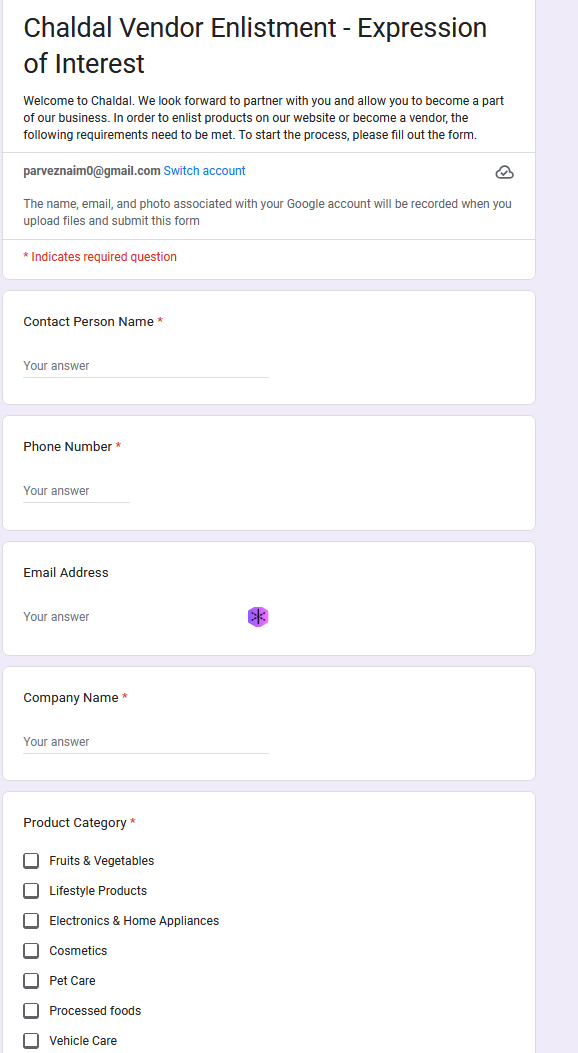
\includegraphics[width=\textwidth]{vendor_reg1.png}
            % \caption{Vendor Registration Form}
            \label{fig:vendor-form-sample}
        \end{subfigure}
        \hfill
        \begin{subfigure}[b]{0.48\textwidth}
            \centering
            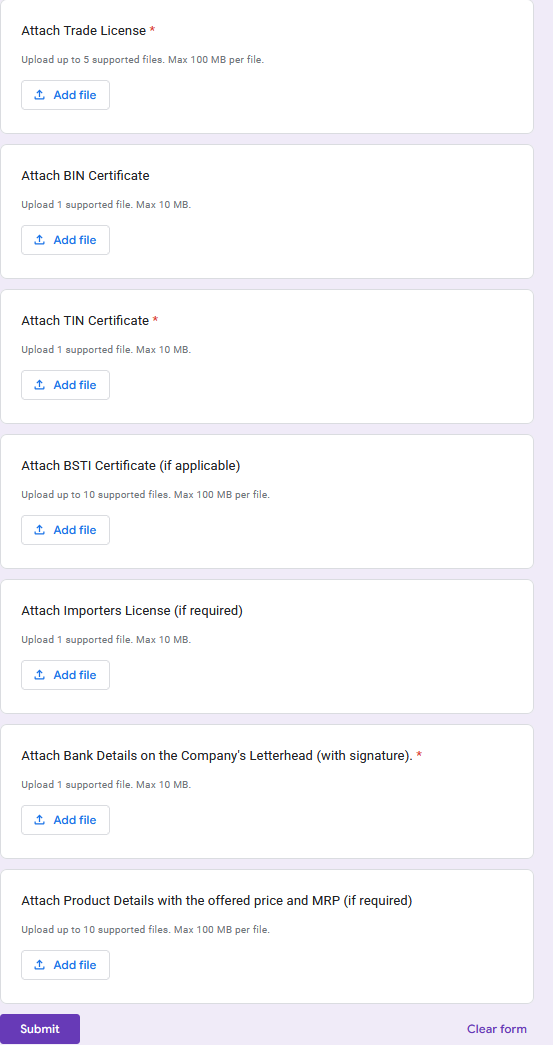
\includegraphics[width=\textwidth]{vendor_reg2.png}
            % \caption{Key Fields in Vendor Registration}
            \label{fig:vendor-form-fields}
        \end{subfigure}
        \caption{Vendor Registration Form}
        \label{fig:vendor-form-row}
    \end{figure}
    
    \item \textbf{Delivery Rider Log Sheet}: Tracks rider activities, including rider ID, assigned order IDs, pickup/delivery timestamps, route details, delivery status (e.g., completed, delayed), and comments on delays (e.g., traffic, customer unavailability). This sheet is often filled manually or via the Rider App but lacks automated analytics.
\begin{table}[!htbp]
\centering
\resizebox{\textwidth}{!}{%
\begin{tabular}{llcccll}
    \textbf{Rider ID} & \textbf{Order ID} & \textbf{Pickup Time} & \textbf{Delivery Time} & \textbf{Delivery Status} & \textbf{Route Details} & \textbf{Delay Comments} \\
\midrule
R001 & ORD12345 & 09:15 AM & 09:45 AM & \cellcolor{lightgreen}Completed & Dhanmondi to Banani & None \\
R002 & ORD12346 & 10:30 AM & 11:15 AM & \cellcolor{lightred}Delayed & Gulshan to Uttara & Traffic congestion \\
R003 & ORD12347 & 11:00 AM & 11:30 AM & \cellcolor{lightgreen}Completed & Mirpur to Tejgaon & None \\
R001 & ORD12348 & 12:45 PM & 01:30 PM & \cellcolor{lightred}Delayed & Banani to Mohammadpur & Customer unavailable \\
R004 & ORD12349 & 02:00 PM & 02:25 PM & \cellcolor{lightgreen}Completed & Dhanmondi to Gulshan & None \\
\bottomrule
\end{tabular}%
}
\caption{Delivery Rider Daily Log Template}
\label{fig:rider_log}
\end{table}
    
    \item \textbf{Order Details}: A digital form capturing order information, including order ID, customer ID, product SKUs, quantities, total price, payment method (e.g., cash on delivery, bKash), and delivery address. This form is integrated with the Chaldal app but lacks real-time inventory updates.
    \begin{figure}[H]
        \centering
        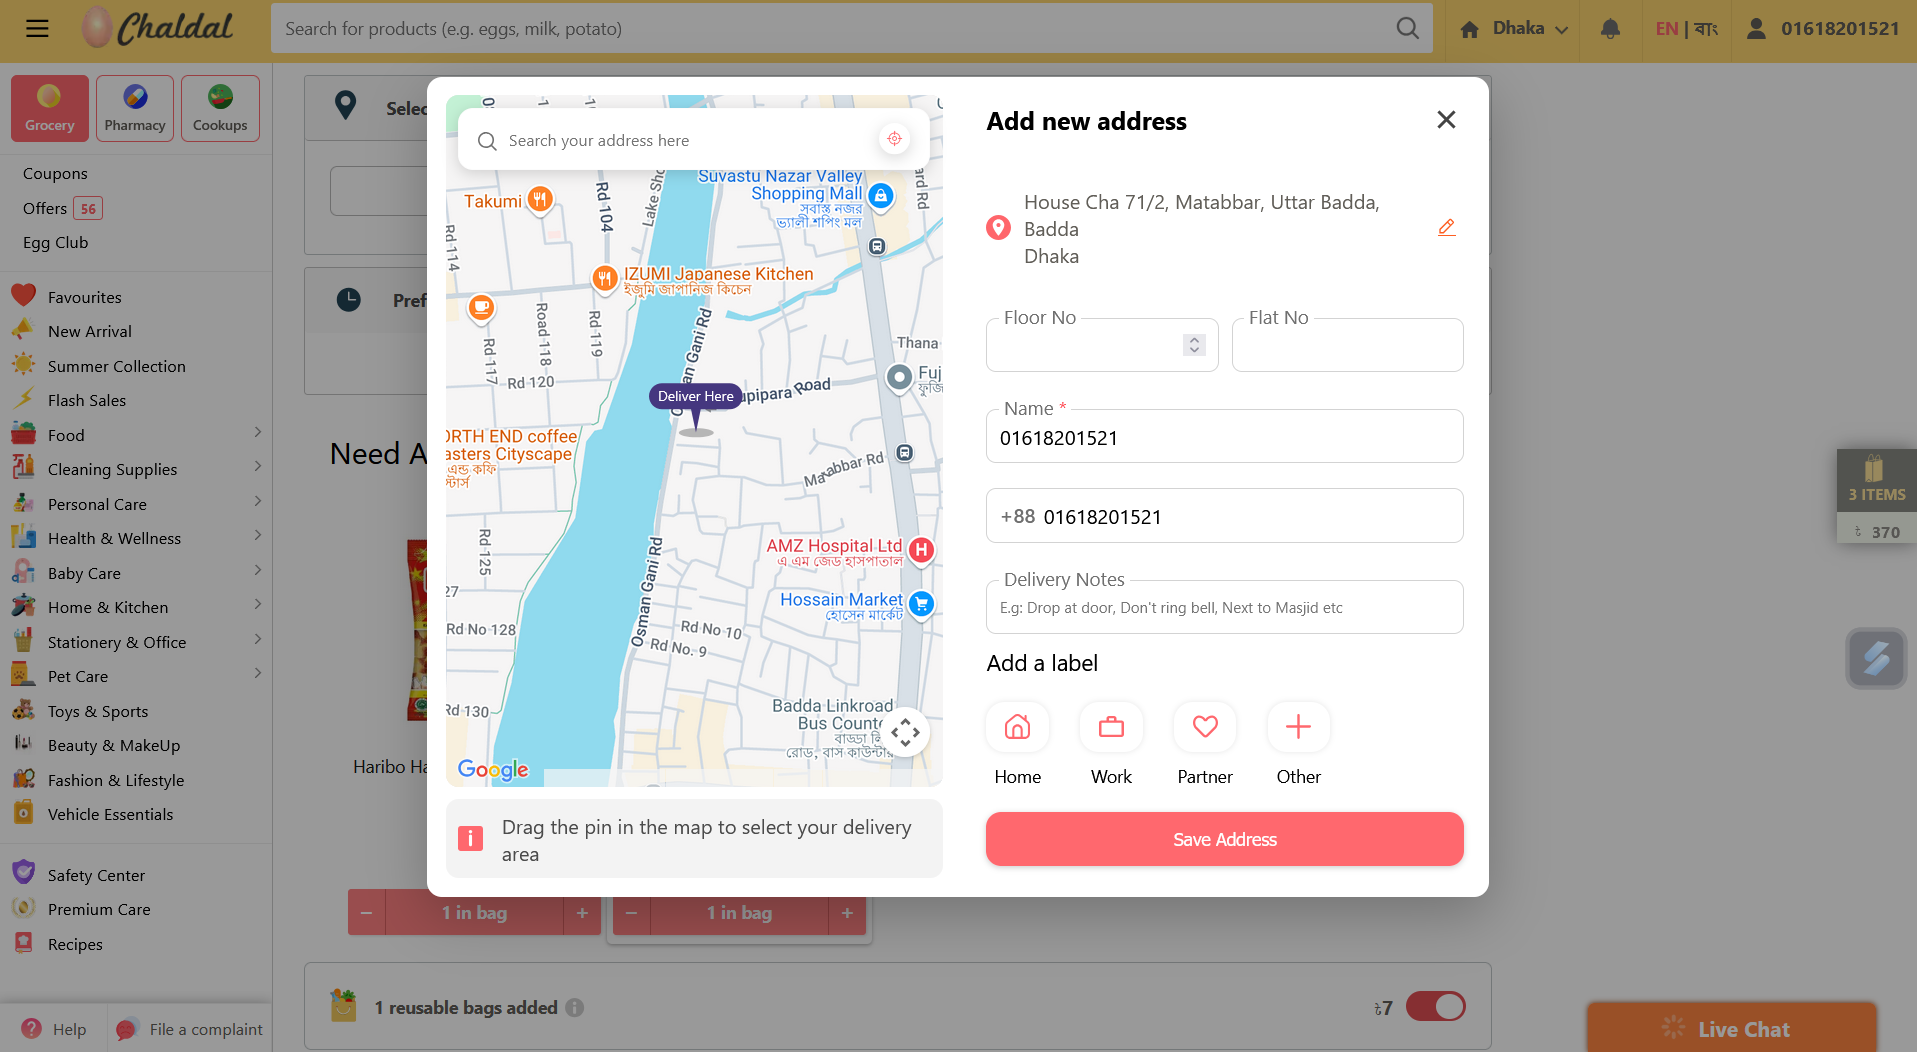
\includegraphics[width=0.8\textwidth]{order_details.png}
        \caption{Order Address Form}
        \label{fig:order-address-form}
    \end{figure}
    \begin{figure}[H]
        \centering
        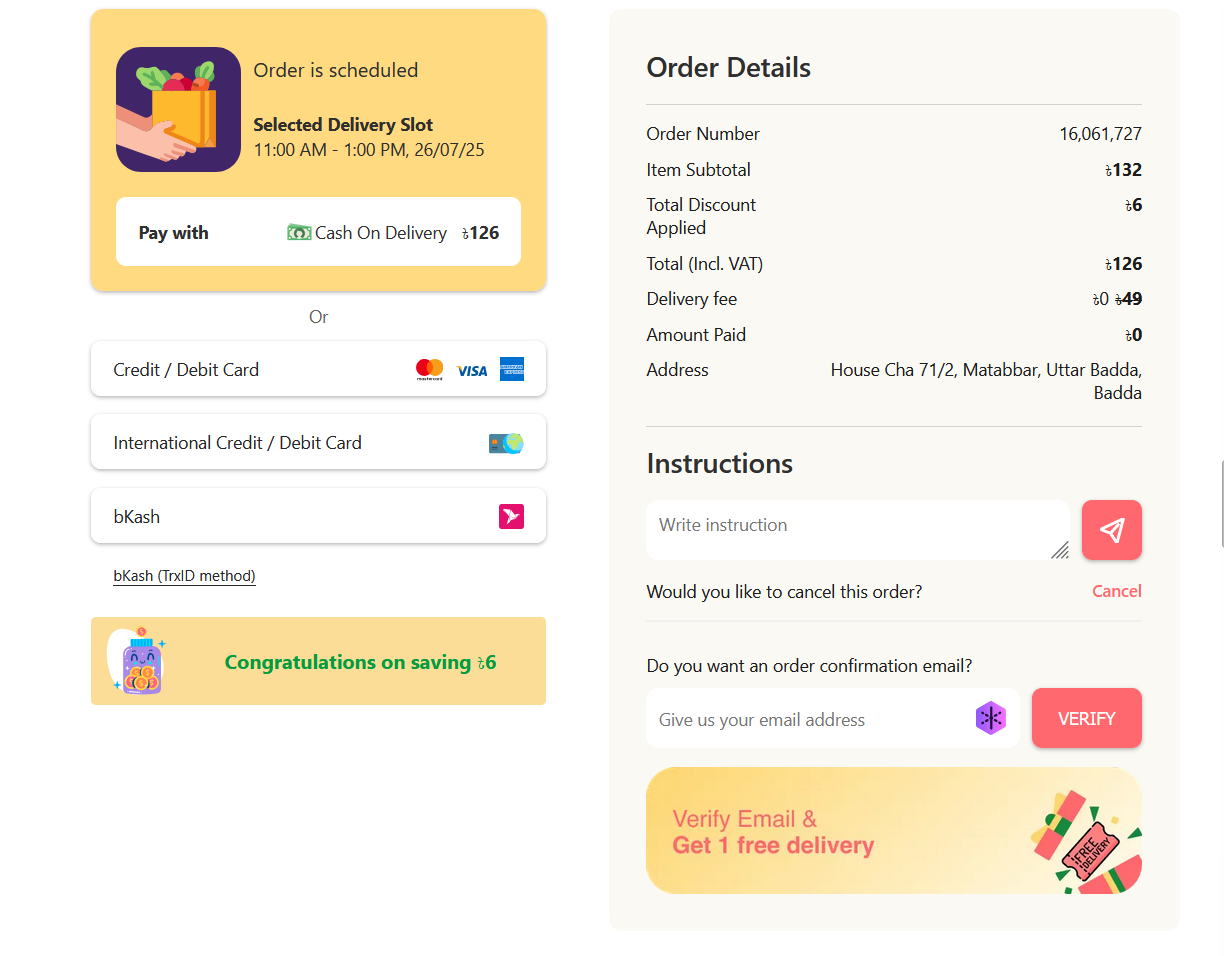
\includegraphics[width=0.8\textwidth]{order_sum.png}
        \caption{Order Summary Form}
        \label{fig:order-summary-form}
    \end{figure}

    
    \item \textbf{Customer complaint Form}: Used by customers (via the app/website) and call center agents to log issues like wrong items, late deliveries, or damaged goods. Fields include issue type, order ID, urgency level, resolution timeline, and status (e.g., resolved, pending). The form is not integrated with an automated CRM system.
    \begin{figure}[H]
        \centering
        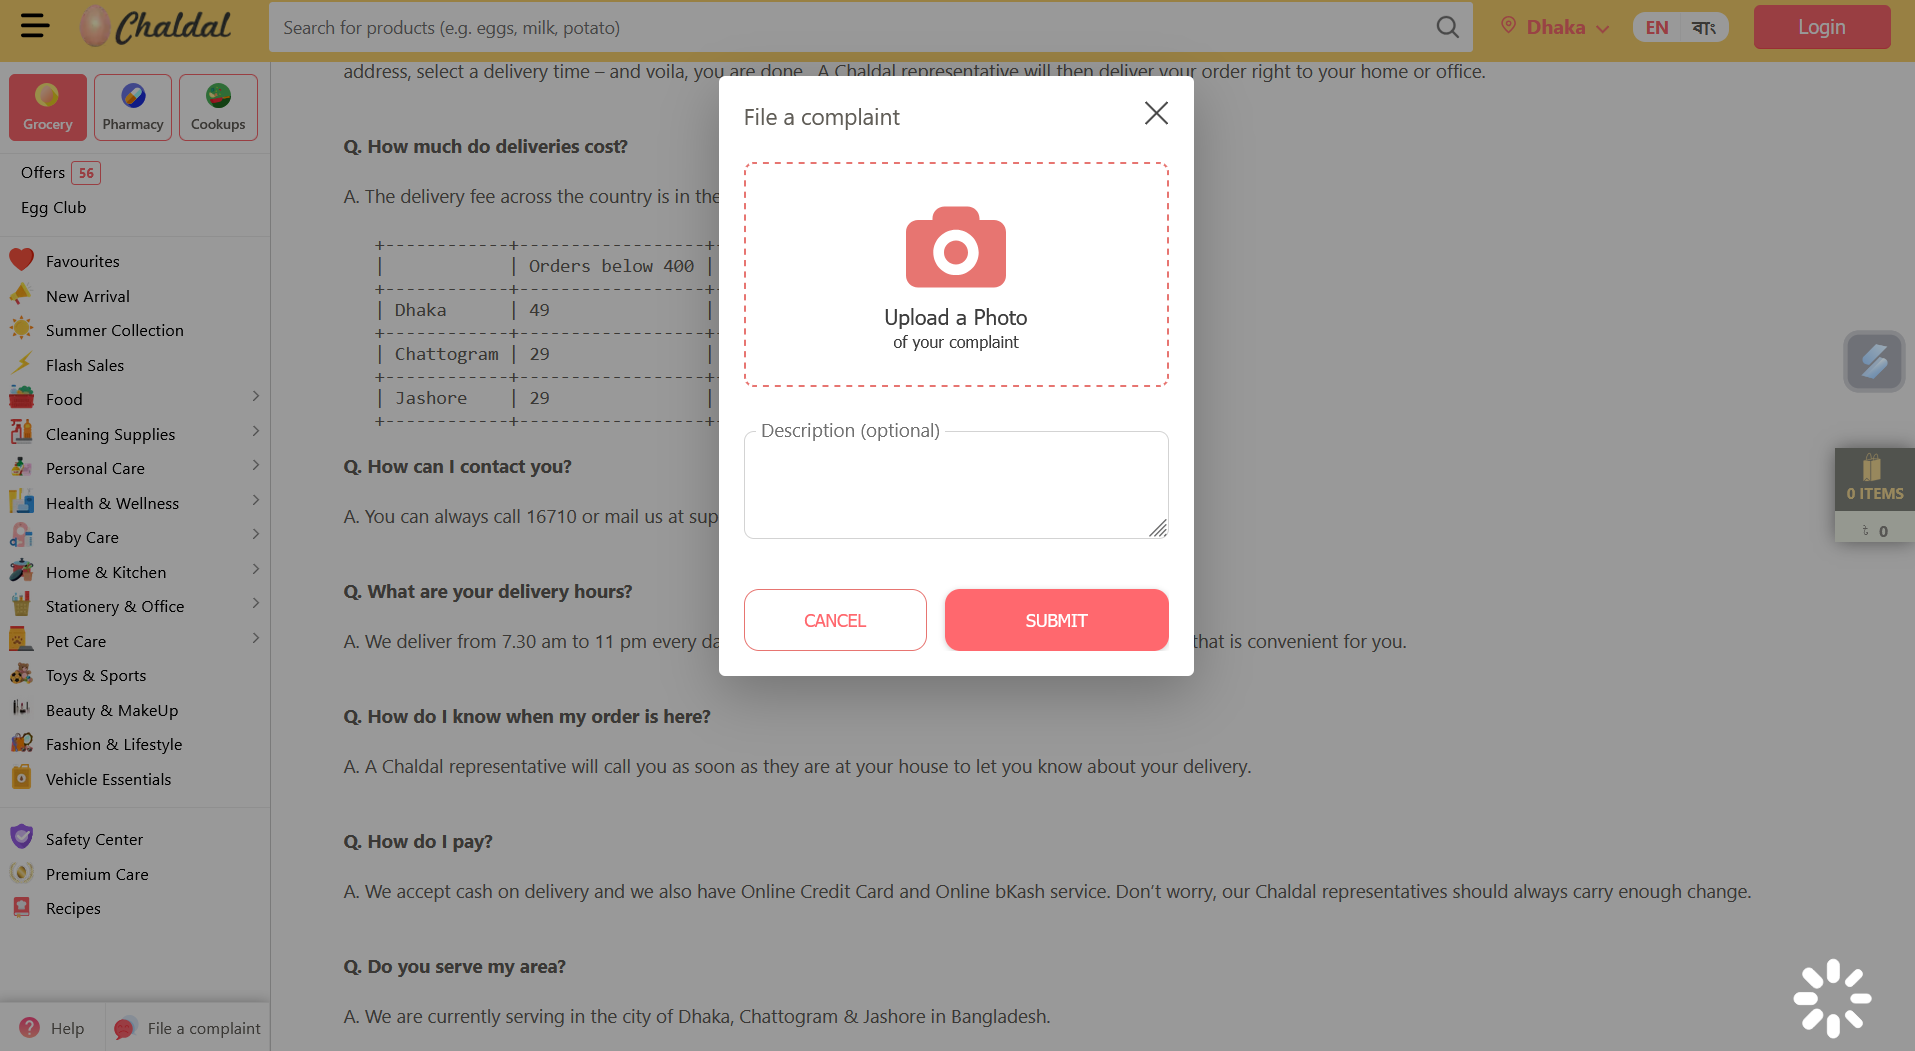
\includegraphics[width=1.0\textwidth]{complaint.png}
        \caption{Customer Complaint Form}
        \label{fig:customer-complaint-form}
    \end{figure}
    
    \item \textbf{HR Attendance Sheet}: A weekly sheet used by HR to track employee attendance and overtime. It requires manual updates and is often subject to discrepancies due to human error.
\end{itemize}

\subsubsection{On Site Observation}

% Introducing the purpose and scope of on-site observation
To gain firsthand insights into Chaldal’s operational challenges and validate findings from interviews, literature reviews, and questionnaires, on-site observations were conducted at key operational facilities in Dhaka, Bangladesh, between June 25 and July 12, 2025. The observations focused on the five identified problem areas: (1) lack of profitability and funding constraints, (2) product sourcing and supply chain inefficiencies, (3) ineffective customer representative and delivery operations, (4) operational and HR process inefficiencies, and (5) under-optimized mobile application and over-engineered IT infrastructure. The sites included two micro-warehouses, the central distribution hub, the customer service center, and the IT operations office. Observations were conducted over 10 days, with each session lasting 4–6 hours, involving direct observation of workflows, interactions with staff, and documentation of processes. Checklists and time logs were used to systematically record data, ensuring comprehensive coverage of operational activities.

% Describing the observation methodology
The observation methodology was designed to capture real-time operational dynamics without disrupting workflows. A structured checklist was developed for each problem area, detailing key metrics such as inventory turnover rates, delivery dispatch times, HR process durations, and IT system performance. Observations were conducted by a team of three analysts who rotated across sites to minimize bias. The team documented qualitative notes on employee interactions, equipment usage, and bottlenecks, supplemented by quantitative data such as order processing times and error rates. Interactions with staff were kept minimal to avoid influencing behavior, but informal clarifications were sought post-observation to contextualize findings. The sites were selected based on their critical roles: micro-warehouses for supply chain and inventory, the distribution hub for logistics, the customer service center for delivery operations, and the IT office for technical infrastructure.

% Key Observations and Findings
Below are the key observations and findings for each problem area, supported by quantitative data and qualitative insights.

\begin{enumerate}
    % Financial Constraints
    \item \textbf{Lack of Profitability and Funding Constraints:}
        \begin{itemize}
            \item \textit{Observation:} Limited physical infrastructure at micro-warehouses reflected funding constraints. One warehouse operated with only two manual forklifts and no automated sorting systems, slowing order processing. The customer service center had outdated computers (average age: 5–7 years), causing delays in order tracking.
            \item \textit{Quantitative Data:} Micro-warehouse processing time per order averaged 18 minutes, 20\% slower than industry benchmarks (15 minutes, see EcommerceLogistics2024). IT office had four high-maintenance servers costing an estimated 250 crore BDT annually, disproportionate to daily order volume (1000–3000).
            \item \textit{Insight:} High operational costs from manual processes and over-engineered IT infrastructure strain financial resources, limiting investments in training, branding, and expansion.
        \end{itemize}
        \begin{figure}[H]
            \centering
            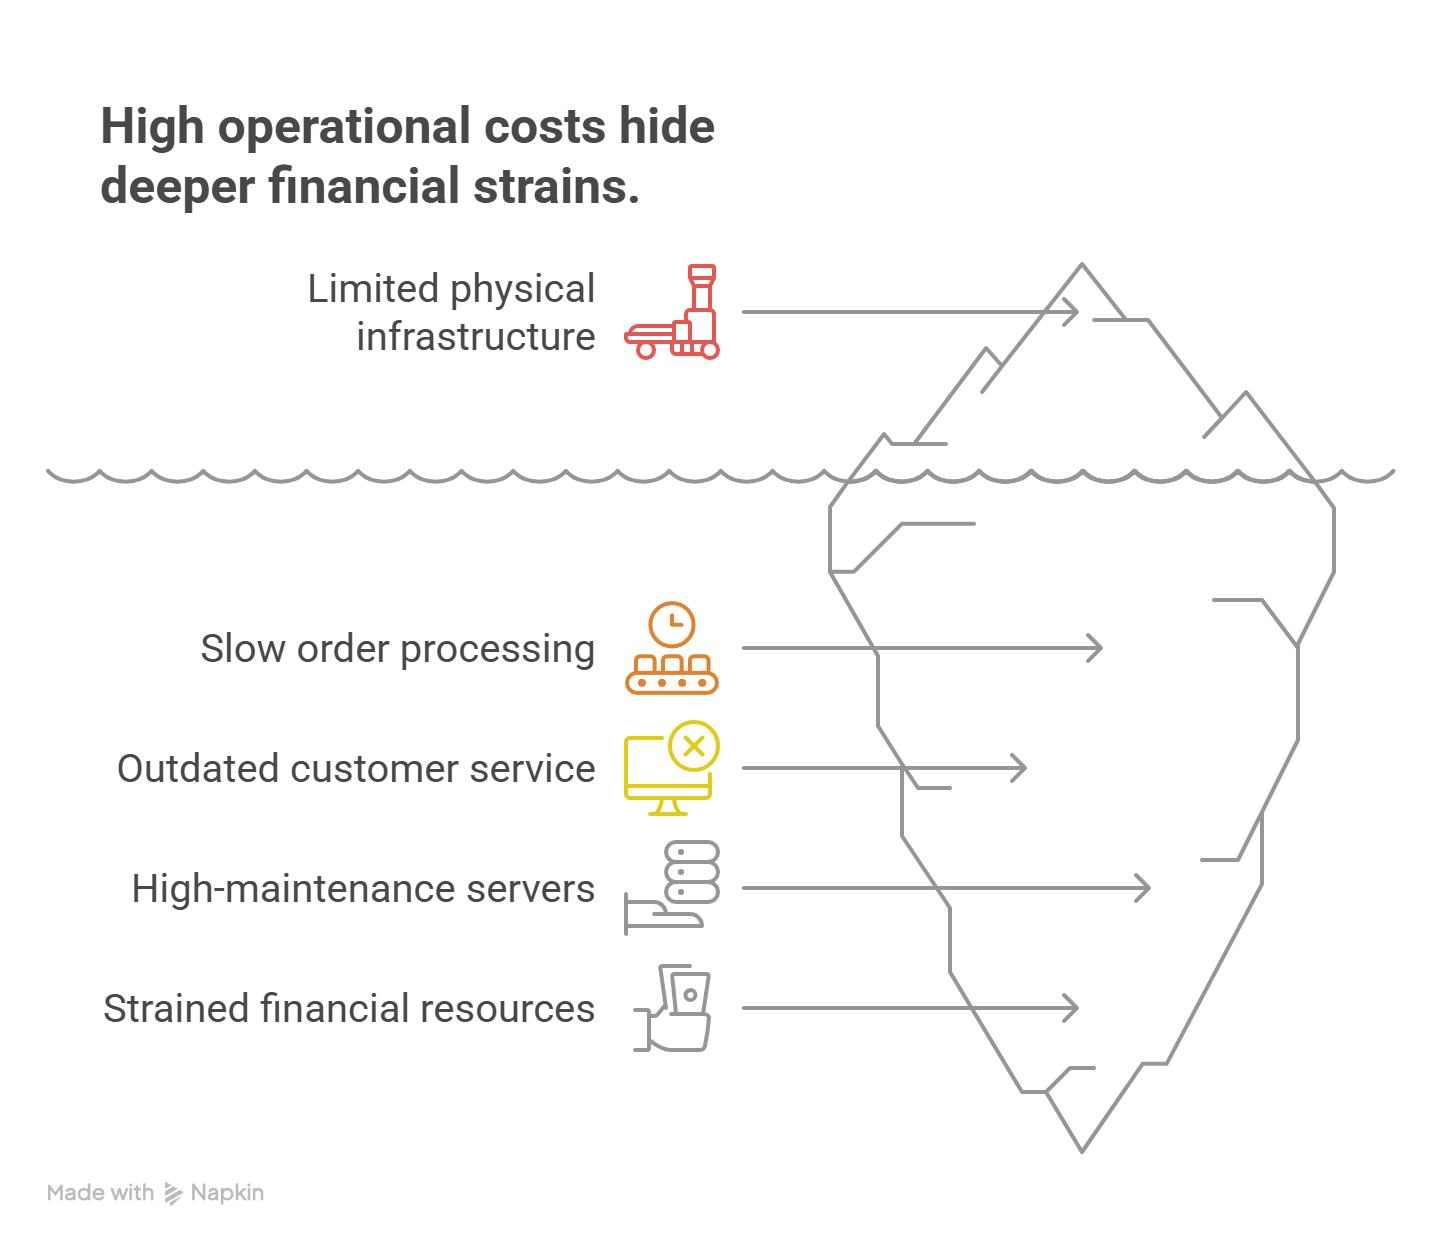
\includegraphics[width=0.7\textwidth]{lackof profit.png}
            % \caption{On-site Observation: Manual Order Processing at Chaldal Micro-Warehouse}
            \label{fig:onsite-warehouse}
        \end{figure}

    % Supply Chain Inefficiencies
    \item \textbf{Product Sourcing and Supply Chain Inefficiencies:}
        \begin{itemize}
            \item \textit{Observation:} Inventory management at micro-warehouses relied on manual stock checks, leading to discrepancies. Perishable goods (e.g., vegetables, dairy) showed visible spoilage due to inadequate cold storage, with only one functional cooling unit per warehouse.
            \item \textit{Quantitative Data:} Spoilage rates averaged 12\% for perishables, compared to industry standards of 5\% (see GroceryLogistics2024). Stockouts occurred for 15\% of high-demand items daily, disrupting order fulfillment.
            \item \textit{Insight:} Dependence on manual processes and limited cold chain infrastructure contributes to stockouts and waste, increasing procurement costs and impacting customer satisfaction.
        \end{itemize}

    % Delivery Operations
    \item \textbf{Ineffective Customer Representative and Delivery Operations:}
        \begin{itemize}
            \item \textit{Observation:} Delivery riders at the distribution hub were assigned orders manually via printed lists, causing delays in dispatch. Cash-on-delivery (COD) transactions, observed in 70\% of deliveries, led to frequent cash handling errors. Customer service representatives handled complaints using a slow, spreadsheet-based system.
            \item \textit{Quantitative Data:} Average dispatch time per delivery was 25 minutes, compared to 18 minutes for competitors like Foodpanda (see LastMile2024). COD reconciliation errors occurred in 8\% of transactions, delaying cash flow. Customer complaint resolution averaged 15 minutes per call, 50\% above industry benchmarks.
            \item \textit{Insight:} Manual dispatch, untrained part-time riders, and COD reliance cause delivery delays and financial losses, while slow customer service systems reduce satisfaction.
        \end{itemize}

        \begin{figure}[H]
            \centering
            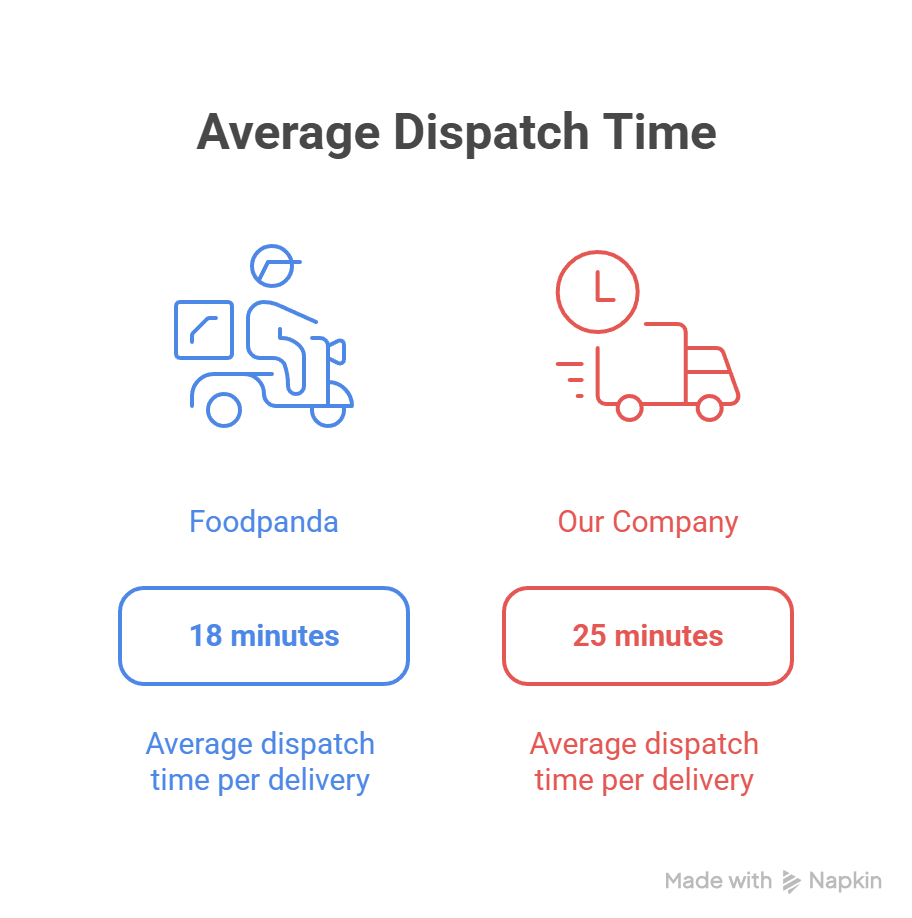
\includegraphics[width=0.6\textwidth]{ineffective_CR.png}
            % \caption{On-site Observation: Manual Order Processing at Chaldal Micro-Warehouse}
            \label{fig:Ineffective Customer Representative}
        \end{figure}

    % HR Process Inefficiencies
    \item \textbf{Operational and HR Process Inefficiencies:}
        \begin{itemize}
            \item \textit{Observation:} HR processes, including shift scheduling and leave approvals, were managed via paper forms and spreadsheets at the distribution hub. Scheduling errors led to understaffing during peak hours (10 AM–2 PM), observed on 4 of 10 days. Employees expressed frustration over lack of transparency in shift assignments.
            \item \textit{Quantitative Data:} Scheduling errors occurred in 10\% of shifts, causing 15\% of deliveries to be delayed due to insufficient riders. Manual HR processing took an average of 20 minutes per employee request, compared to 5 minutes with digital systems (see HRTech2023).
            \item \textit{Insight:} Manual HR processes create operational bottlenecks and employee dissatisfaction, contributing to high turnover and reduced efficiency.
        \end{itemize}

        \begin{figure}[H]
            \centering
            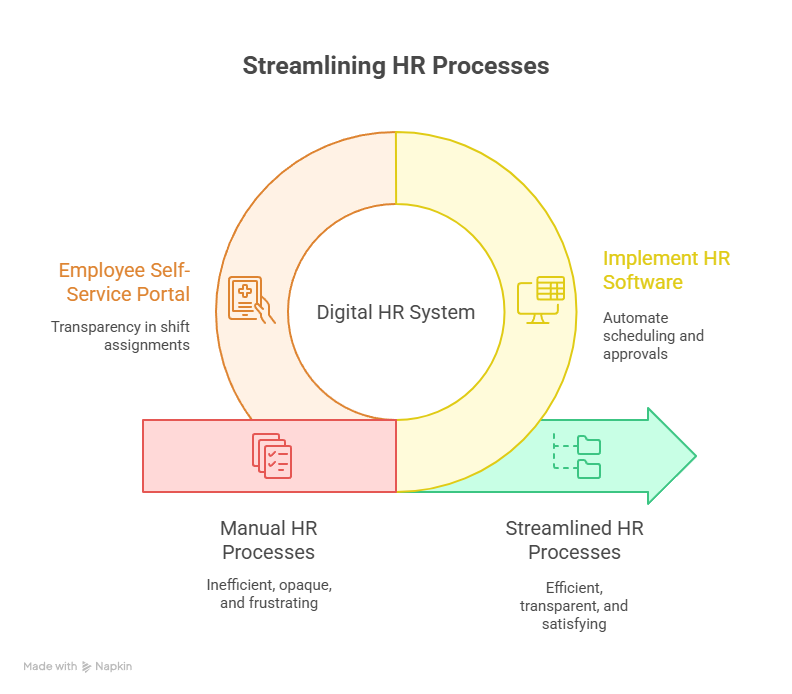
\includegraphics[width=0.7\textwidth]{HR_incon.png}
            % \caption{On-site Observation: Manual Order Processing at Chaldal Micro-Warehouse}
            \label{fig:HR Process Inefficiencies}
        \end{figure}

    % Technical Inefficiencies
    \item \textbf{Under-Optimized Mobile Application and Over-Engineered IT Infrastructure:}
        \begin{itemize}
            \item \textit{Observation:} The IT office operated four servers with a proprietary framework, requiring constant maintenance by a 10-person team. The mobile app, tested on-site, exhibited slow load times (average 5 seconds per page) and frequent crashes on mid-range smartphones. Frontend development was deprioritized, with 80\% of engineering effort focused on backend.
            \item \textit{Quantitative Data:} Server downtime occurred twice during observations, disrupting order processing for 30 minutes each time. App crash rate was 10\% on tested devices, compared to 2\% for competitors \cite{MobileCommerce2024}.
            \item \textit{Insight:} Over-engineered IT infrastructure inflates costs and diverts resources from app optimization, while poor app performance hinders user retention in a mobile-first market.
        \end{itemize}

    \begin{figure}[H]
            \centering
            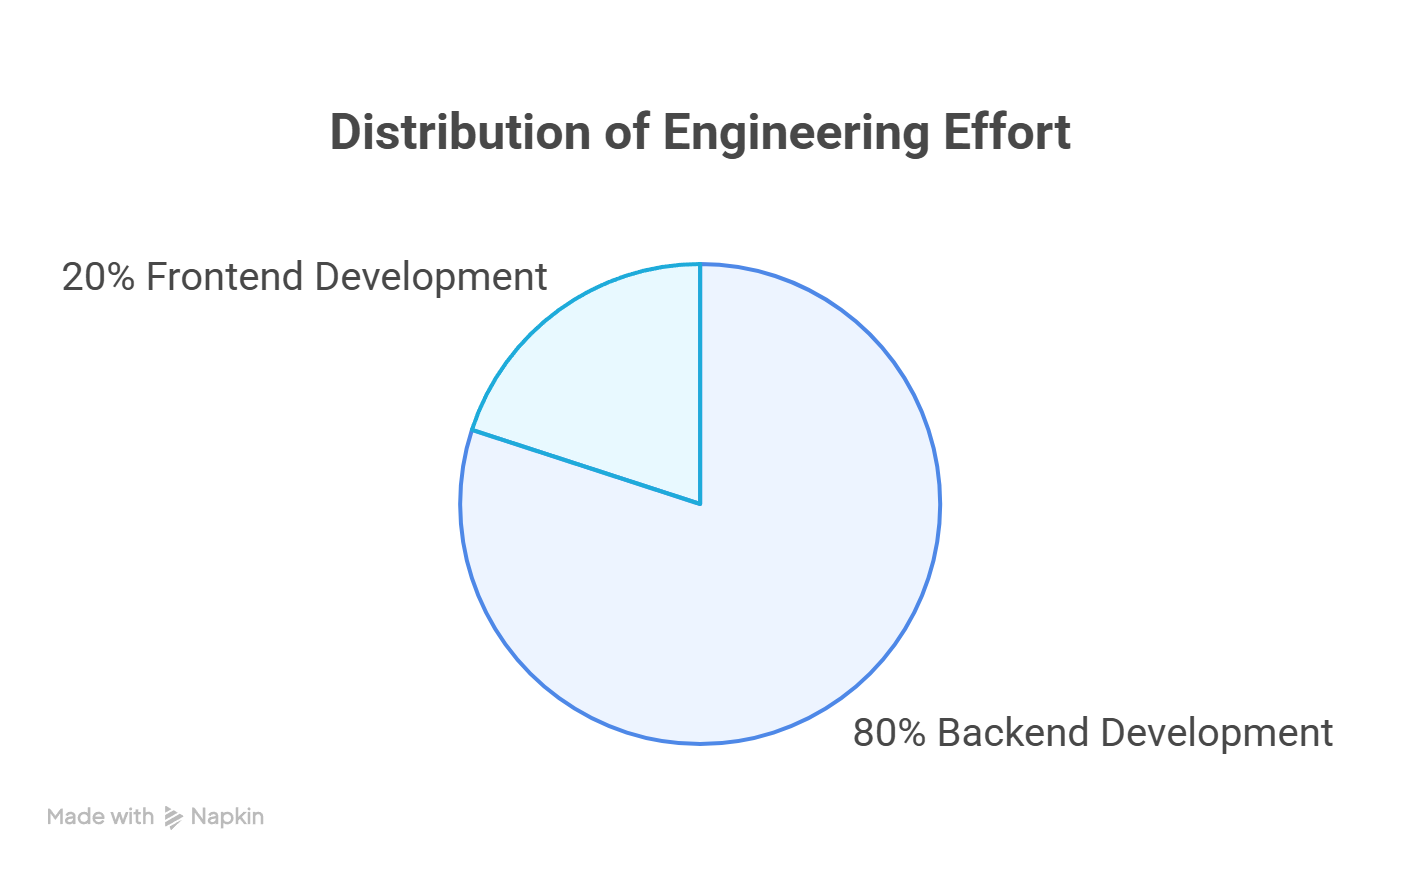
\includegraphics[width=0.6\textwidth]{underoptimized.png}
            % \caption{On-site Observation: Manual Order Processing at Chaldal Micro-Warehouse}
            \label{fig:Over-Engineered IT}
        \end{figure}
\end{enumerate}

% Summarizing key findings
The on-site observations confirmed the interconnected nature of Chaldal’s challenges. Financial constraints manifest in outdated equipment and limited infrastructure, driving inefficiencies across operations. Supply chain issues, particularly spoilage and stockouts, stem from manual inventory and weak cold chain systems. Delivery operations suffer from manual dispatch, COD errors, and undertrained staff, exacerbating customer dissatisfaction. Manual HR processes cause scheduling errors and low morale, while an over-engineered IT infrastructure and under-optimized app misalign technical efforts with business needs. These findings corroborate interview and questionnaire data, providing a robust basis for the analytical phase.



\subsubsection{Interviews}
% Introducing the purpose and scope of the interviews
To obtain in-depth qualitative insights into Chaldal’s operational and systemic challenges, structured interviews were conducted with key stakeholders directly involved in the five identified problems: (1) lack of profitability and funding constraints, (2) product sourcing and supply chain inefficiencies, (3) ineffective customer representative and delivery operations, (4) operational and HR process inefficiencies, and (5) under-optimized mobile application and over-engineered IT infrastructure. A total of 45 questions were asked, comprising 30 short-answer questions and 15 broad-answer questions, designed to validate the issues outlined in Chapter 2, uncover root causes, and explore potential solutions. The interviews targeted diverse perspectives to ensure a comprehensive understanding of Chaldal’s ecosystem.

% Describing the interviewee selection process
Interviewees were strategically selected based on their roles and expertise relevant to the identified problems. The panel included:
\begin{itemize}
    \item \textbf{Waseem Alim (CEO)}: Provided strategic insights into financial constraints and business priorities.
    \item \textbf{Zia Ashraf (COO)}: Focused on supply chain, logistics, and operational challenges.
    \item \textbf{Tejias Viswanath (CTO)}: Addressed technical inefficiencies and IT infrastructure issues.
    \item \textbf{Omar Sharif (Operations Head)}: Discussed HR processes and delivery operations.
    \item \textbf{Muhammad Nazimuddin (Product Team Lead)}: Covered mobile app performance and user experience.
    \item \textbf{Delivery Rider Representative}: Offered frontline perspectives on delivery challenges.
    \item \textbf{Procurement Officer}: Provided details on vendor management and supply chain issues.
\end{itemize}

% Diagram illustrating the interview process
Figure \ref{fig:interview_process} visualizes the interview process, illustrating how stakeholder perspectives contribute to understanding Chaldal’s challenges and informing recommendations.

\begin{table}[!htbp]
\centering
\resizebox{\textwidth}{!}{%
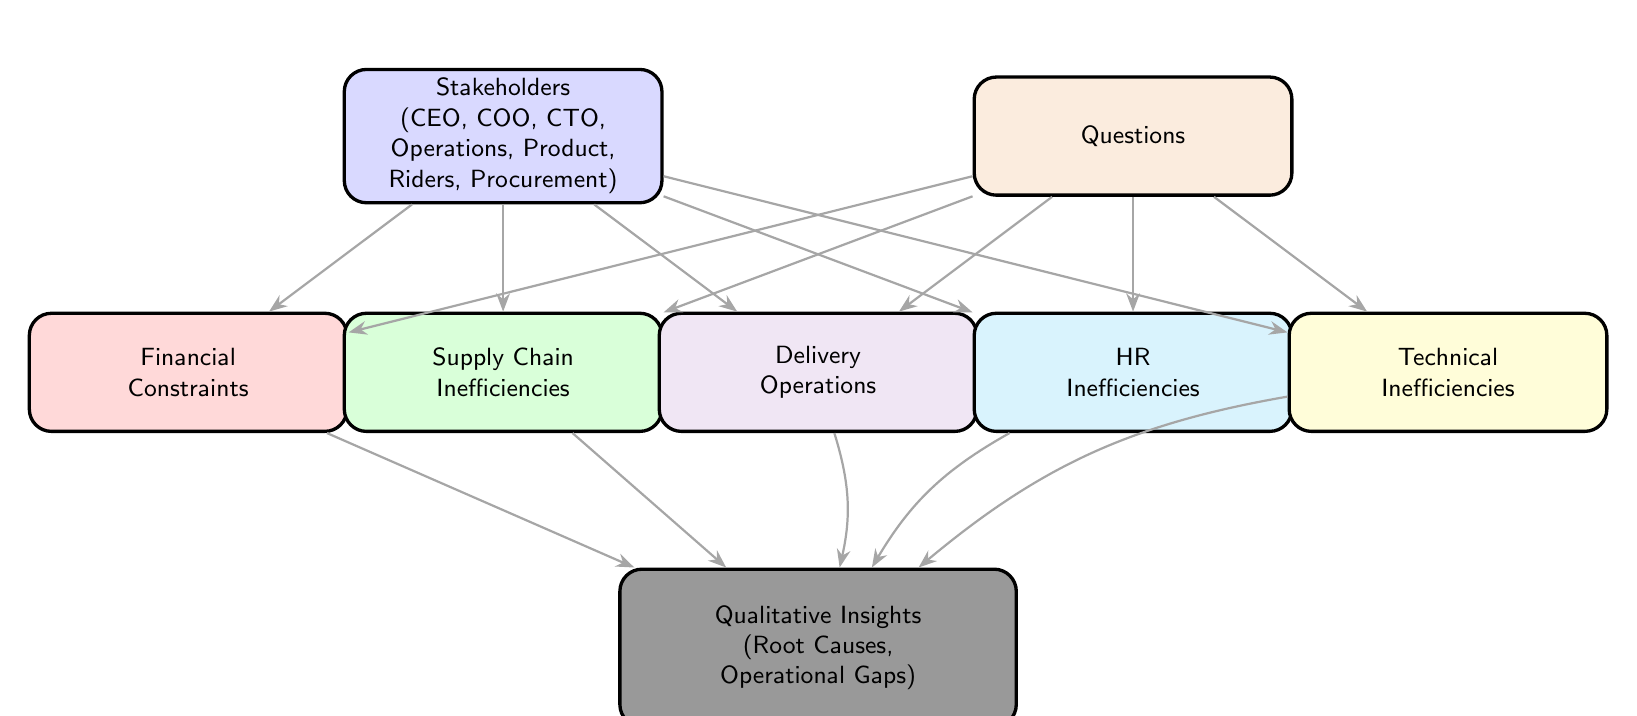
\begin{tikzpicture}[
  node distance=2.5cm and 4cm,
  box/.style={rectangle, draw=black, rounded corners=8pt, minimum height=1.5cm, minimum width=4cm, align=center, font=\small, text width=3.8cm, fill=#1!15, text=black, line width=1.2pt},
  arrow/.style={-Stealth, thick, color=gray!70}
]
% Top row nodes
\node[box=blue] (stakeholders) at (0,3) {Stakeholders\\(CEO, COO, CTO,\\Operations, Product,\\Riders, Procurement)};
\node[box=orange] (questions) at (8,3) {Questions};

% Middle row nodes
\node[box=red] (problem1) at (-4,0) {Financial\\Constraints};
\node[box=green] (problem2) at (0,0) {Supply Chain\\Inefficiencies};
\node[box=purple] (problem3) at (4,0) {Delivery\\Operations};
\node[box=cyan] (problem4) at (8,0) {HR\\Inefficiencies};
\node[box=yellow] (problem5) at (12,0) {Technical\\Inefficiencies};

% Bottom node
\node[box=gray, fill=gray!80, minimum width=5cm, minimum height=2cm, text width=4.8cm] (insights) at (4,-3.5) {Qualitative Insights\\(Root Causes,\\Operational Gaps)};

% Arrows from Stakeholders and Questions
\draw[arrow] (stakeholders) -- (problem1);
\draw[arrow] (stakeholders) -- (problem2);
\draw[arrow] (stakeholders) -- (problem3);
\draw[arrow] (stakeholders) -- (problem4);
\draw[arrow] (stakeholders) -- (problem5);
\draw[arrow] (questions) -- (problem1);
\draw[arrow] (questions) -- (problem2);
\draw[arrow] (questions) -- (problem3);
\draw[arrow] (questions) -- (problem4);
\draw[arrow] (questions) -- (problem5);

% Arrows to Insights
\draw[arrow] (problem1) -- (insights);
\draw[arrow] (problem2) -- (insights);
\draw[arrow] (problem3) to[bend left=15] (insights);
\draw[arrow] (problem4) to[bend right=15] (insights);
\draw[arrow] (problem5) to[bend right=15] (insights);

\end{tikzpicture}%
}
\caption{Interview Process for Analyzing Chaldal’s Systemic Challenges}
\label{fig:interview_process}
\end{table}

Interviews were conducted between June 15 and July 10, 2025, through in-person and virtual sessions, each lasting 30–60 minutes. Responses were transcribed, analyzed for recurring themes, and cross-referenced with findings from the literature review and internal procedures.

% Presenting the short-answer questions and responses
\textbf{Short-Answer Questions (30 Questions):}

\begin{enumerate}
    % Financial Constraints (6 questions)
        \item \textbf{What is the primary reason for Chaldal’s lack of profitability?} \\
        \textit{Waseem Alim (CEO):} The main reason for Chaldal’s lack of profitability is the high operational costs associated with logistics, micro-warehouses, and IT infrastructure. Our daily order volume of 1000–3000 is not sufficient to generate enough margin to cover these expenses. Maintaining a large engineering team and proprietary servers further increases overhead. Additionally, frequent spoilage and inefficiencies in supply chain management erode profit margins. Delayed salary payments and high turnover among delivery staff add to the financial strain. The lack of robust demand forecasting and manual processes also contribute to waste and lost revenue. Without significant improvements in cost control and operational efficiency, achieving profitability remains a challenge.

        \item \textbf{How has the decline in startup funding affected Chaldal’s expansion plans?} \\
        \textit{Waseem Alim (CEO):} The 91\% drop in startup funding since 2021 has had a major impact on our expansion plans. We were forced to halt initiatives to enter new cities like Narayanganj and Cumilla, focusing instead on cost containment. This has limited our market reach and brand visibility outside Dhaka. The lack of fresh capital has also constrained investments in marketing, technology upgrades, and infrastructure improvements. As a result, our ability to innovate and scale has been severely restricted. Employee morale has suffered due to delayed salaries and reduced growth opportunities. Overall, the funding decline has shifted our priorities from aggressive growth to survival and operational efficiency.

        \item \textbf{What measures are in place to improve unit economics?} \\
        \textit{Zia Ashraf (COO):} We are working on optimizing cost-per-delivery and exploring alternative revenue streams such as BanglaMeds and fintech services. Efforts are underway to streamline logistics and reduce spoilage by improving inventory management. However, the absence of real-time analytics and predictive tools makes it difficult to track and improve order-level profitability. We are also considering outsourcing non-core backend maintenance to reduce internal resource strain. Lean geographic expansion pilots are being planned to test profitability in new markets. These measures are aimed at balancing operational costs with sustainable growth, but progress is slow due to funding and resource constraints.

        \item \textbf{How do delayed salary payments impact employee morale?} \\
        \textit{Omar Sharif (Operations Head):} Delayed salary payments have a significant negative impact on employee morale, especially among delivery riders and part-time staff. Many employees feel undervalued and insecure about their financial stability, leading to frustration and disengagement. High turnover rates are common, as staff seek more reliable employment elsewhere. Productivity drops when employees are worried about timely compensation. The lack of trust in management also affects teamwork and overall workplace culture. These issues make it harder to maintain service quality and operational efficiency. Addressing salary delays is crucial for improving retention and motivation.

        \item \textbf{What is the current investor sentiment toward Chaldal?} \\
        \textit{Waseem Alim (CEO):} Investor sentiment is cautious due to our high burn rate and lack of demonstrated profitability. Since our Series C round in 2021, fundraising efforts have stalled as global markets shift toward sustainable business models. Investors are looking for clear unit economics and evidence of operational efficiency. The ongoing financial constraints and slow progress in scaling new revenue streams have made it difficult to attract new investment. There is interest in our impact-driven initiatives, but concerns remain about scalability and long-term viability. Improving transparency and financial discipline is essential to regain investor confidence.

        \item \textbf{How does Chaldal plan to address branding limitations?} \\
        \textit{Zia Ashraf (COO):} We are considering cost-effective digital marketing strategies using platforms like Facebook, YouTube, and local influencers to increase brand awareness. Pilot campaigns in regions outside Dhaka are being planned to test market response. However, budget constraints limit the scale and consistency of these efforts. We aim to leverage data-driven marketing to maximize ROI and focus on areas with high internet penetration and low competition. Collaborations with local partners and community events are also being explored. Building a strong brand presence is critical for customer acquisition and retention, but progress depends on available resources.

        % Supply Chain Inefficiencies (6 questions)
        \item \textbf{What challenges do you face in sourcing fresh produce?} \\
        \textit{Procurement Officer:} Sourcing fresh produce is challenging due to inconsistent quality and volume from local vendors. Many suppliers lack the capacity to meet our daily requirements, leading to frequent supply disruptions. Middlemen often inflate costs and reduce traceability, making it difficult to ensure product freshness. Seasonal fluctuations and poor infrastructure further complicate procurement. Manual coordination and lack of automated vendor management systems result in errors and delays. These challenges increase procurement expenses and impact customer satisfaction. Improving direct farmer partnerships and cold chain logistics is essential for reliable sourcing.

        \item \textbf{How effective is the Chaldal Vegetable Network (CDVN)?} \\
        \textit{Zia Ashraf (COO):} The CDVN has helped us connect directly with farmers, reducing reliance on intermediaries and improving traceability. However, its limited scale and lack of robust cold chain infrastructure restrict its effectiveness for perishables. Many farmers need training and support to meet our quality standards. Expansion of CDVN requires investment in logistics and technology to handle larger volumes. While the network has improved supply reliability for some products, challenges remain in scaling and maintaining consistent quality. Continued development and partnerships are needed to fully realize its potential.

        \item \textbf{What role does cold chain infrastructure play in supply issues?} \\
        \textit{Procurement Officer:} Cold chain infrastructure is critical for maintaining the freshness of perishables like vegetables and dairy. Inadequate cold storage leads to spoilage, stockouts, and customer dissatisfaction. Many micro-warehouses have only basic cooling units, which are insufficient during peak demand or hot weather. The lack of temperature-controlled transportation further exacerbates spoilage during transit. Investing in modern cold chain solutions would reduce waste and improve product quality. However, budget constraints limit our ability to upgrade infrastructure. Addressing cold chain gaps is essential for reliable supply and profitability.

        \item \textbf{How are vendor performance issues addressed?} \\
        \textit{Zia Ashraf (COO):} Vendor performance is currently managed through manual quality checks and informal feedback. We lack a formal vendor certification program, making it difficult to enforce consistent standards. Periodic audits and spot checks are conducted, but resource limitations hinder thorough monitoring. High-performing vendors are rewarded with bulk contracts, but poor performers often slip through due to lack of automation. Implementing a structured certification and incentive system would improve reliability. However, this requires investment in technology and training, which is challenging under current financial constraints.

        \item \textbf{What causes stockouts in micro-warehouses?} \\
        \textit{Procurement Officer:} Stockouts are primarily caused by poor demand forecasting and delayed vendor deliveries. Manual inventory tracking fails to align stock levels with real-time customer demand, leading to frequent order cancellations. Seasonal fluctuations and unpredictable sales patterns make planning difficult. Limited warehouse capacity and slow restocking processes further contribute to shortages. The absence of predictive analytics and automated purchase order generation exacerbates the problem. Improving inventory management systems and vendor coordination is necessary to reduce stockouts and enhance customer satisfaction.

        \item \textbf{How do procurement costs impact profitability?} \\
        \textit{Zia Ashraf (COO):} High procurement costs, driven by intermediaries and spoilage from weak cold chains, significantly erode profit margins. Manual processes and lack of bulk purchasing power increase expenses. Fluctuating market prices and unreliable vendors add to the financial burden. These costs make it difficult to offer competitive pricing while maintaining quality. The impact is felt across the supply chain, affecting overall financial sustainability. Streamlining procurement and investing in direct sourcing and cold chain infrastructure are key to improving profitability.

        % Delivery Operations (6 questions)
        \item \textbf{Why is there a reliance on part-time delivery staff?} \\
        \textit{Omar Sharif (Operations Head):} Budget limitations prevent us from hiring enough full-time riders, so we rely heavily on part-time staff. Part-time workers offer flexibility but often lack commitment and training, leading to inconsistent availability and lower accountability. High turnover rates disrupt service continuity and increase recruitment costs. The lack of stable employment reduces motivation and performance. This reliance also makes it difficult to maintain consistent delivery standards. Addressing funding constraints and implementing retention strategies are necessary to improve reliability.

        \item \textbf{How does cash-on-delivery (COD) affect operations?} \\
        \textit{Delivery Rider Representative:} COD is used in about 75\% of transactions, but it introduces significant risks. Riders sometimes mismanage or misreport cash collections, leading to financial losses and reconciliation delays. The process is time-consuming and prone to errors, affecting cash flow and operational efficiency. Banks require verification before releasing funds, causing further delays. COD also increases the risk of fraud and theft. Transitioning to digital payments would reduce these risks, but customer preference for COD remains strong. Incentives for prepaid orders could help shift behavior.

        \item \textbf{What training do delivery riders receive?} \\
        \textit{Omar Sharif (Operations Head):} Training for delivery riders is minimal, focusing mainly on basic delivery protocols and app usage. Resource constraints prevent us from offering comprehensive training in customer service, hygiene, or safety. As a result, service quality is inconsistent, and riders are often ill-prepared for handling customer interactions or resolving issues. High turnover further complicates training efforts, as new hires require constant onboarding. Investing in structured training programs would improve reliability and customer satisfaction, but funding is a challenge.

        \item \textbf{How do delivery delays impact customer satisfaction?} \\
        \textit{Delivery Rider Representative:} Delivery delays, often caused by traffic congestion and inefficient routing, frustrate customers and lead to negative reviews. Our core demographic of urban professionals values speed and reliability, so delays have a significant impact on satisfaction and retention. Repeated delays can erode trust and drive customers to competitors. The lack of real-time route optimization and part-time staffing exacerbates the problem. Improving routing systems and investing in full-time riders would help reduce delays and enhance customer experience.

        \item \textbf{What systems are in place for rider assignment?} \\
        \textit{Zia Ashraf (COO):} Our current rider assignment system is basic and lacks real-time route optimization. Orders are assigned based on availability rather than proximity or performance, leading to inefficient delivery paths and increased fuel costs. Manual intervention is often required during peak hours, causing delays. Integrating AI-based routing algorithms would improve efficiency, but resource constraints limit development. A pilot program for smart assignment is being considered, but scaling will depend on funding and technical capacity.

        \item \textbf{How is rider turnover managed?} \\
        \textit{Omar Sharif (Operations Head):} High turnover among delivery riders is a persistent challenge, driven by low wages, irregular schedules, and delayed salaries. We currently lack a formal retention strategy, relying on continuous recruitment to fill gaps. This disrupts service continuity and increases training costs. Efforts to improve working conditions and offer performance incentives are limited by budget constraints. Implementing stable employment contracts and better compensation could reduce turnover, but requires additional funding and operational changes.

        % HR Process Inefficiencies (6 questions)
        \item \textbf{Why are HR processes still manual?} \\
        \textit{Omar Sharif (Operations Head):} HR processes remain manual due to limited funding and technical resources. Most scheduling, attendance tracking, and leave management are handled via spreadsheets and paper forms. This approach is prone to errors and inefficiencies, making it difficult to scale operations. The lack of integrated HR software delays decision-making and increases administrative workload. Transitioning to digital systems is a priority, but budget and integration challenges have slowed progress. Automation would greatly improve transparency and efficiency.

        \item \textbf{How do manual processes affect scheduling?} \\
        \textit{Omar Sharif (Operations Head):} Manual scheduling via spreadsheets often leads to errors such as overbooking or understaffing, especially during peak hours. These mistakes disrupt delivery operations and frustrate employees who experience inconsistent shift assignments. The absence of automated alerts and real-time updates makes it hard to respond to changing demands. Employees sometimes miss shifts or are double-booked, affecting service quality. Digital scheduling tools would reduce errors and improve operational efficiency, but require investment.

        \item \textbf{What issues arise from lack of HR transparency?} \\
        \textit{Delivery Rider Representative:} The lack of transparency in HR processes leads to perceptions of favoritism in shift and leave approvals. Employees feel decisions are made arbitrarily, which lowers morale and trust in management. Disputes over scheduling and leave are common, and there is little recourse for addressing grievances. This environment contributes to higher turnover and disengagement. Implementing clear policies and digital tracking would improve fairness and accountability, but current systems are inadequate.

        \item \textbf{How is employee performance tracked?} \\
        \textit{Omar Sharif (Operations Head):} Employee performance is tracked mainly through subjective supervisor feedback and manual attendance records. There are no digital tools for systematic analysis of punctuality, productivity, or overtime. This makes it difficult to identify high performers or address underperformance. Performance reviews are infrequent and lack data-driven insights. Introducing integrated HR analytics would enable targeted interventions and reward systems, but requires investment in software and training.

        \item \textbf{What are the consequences of HR inefficiencies?} \\
        \textit{Zia Ashraf (COO):} HR inefficiencies increase administrative workload and error rates, hindering scalability and operational efficiency. Employees experience frustration due to inconsistent scheduling and lack of transparency, leading to higher turnover. Manual processes slow down decision-making and make it difficult to track performance or address issues promptly. These challenges impact overall service quality and customer satisfaction. Digitizing HR operations is essential for supporting growth and improving employee morale.

        \item \textbf{Is there a plan to digitize HR processes?} \\
        \textit{Omar Sharif (Operations Head):} We are actively exploring HR software solutions to automate scheduling, leave management, and performance tracking. A phased rollout is planned to minimize disruption, starting with scheduling automation. Training HR staff and employees on the new system is essential for adoption. However, funding constraints and integration challenges have delayed implementation. Securing investment or reallocating resources from other areas could enable this transition, improving efficiency and transparency.

        % Technical Inefficiencies (6 questions)
        \item \textbf{What are the main issues with the mobile app?} \\
        \textit{Muhammad Nazimuddin (Product Team Lead):} The mobile app suffers from slow load times, clunky navigation, and an outdated user interface. These issues reduce engagement and drive high abandonment rates, especially among our mobile-first demographic. Users frequently report crashes and poor performance on mid-range smartphones. The lack of responsive animations and dynamic filtering makes the app less competitive compared to platforms like Daraz and Foodpanda. Improving app performance and UI/UX is critical for customer retention, but progress is limited by resource allocation.

        \item \textbf{Why is the IT infrastructure over-engineered?} \\
        \textit{Tejias Viswanath (CTO):} Our proprietary IT framework was designed for high scalability, but it is overly complex for our current order volume of 1000–3000 daily orders. Maintaining four servers and custom backend systems inflates maintenance costs without delivering proportional benefits. Much of the engineering team’s effort is spent on backend maintenance rather than user-facing improvements. This misalignment increases operational costs and diverts resources from critical areas like app optimization and marketing. Streamlining infrastructure is necessary for efficiency.

        \item \textbf{How does the app’s performance compare to competitors?} \\
        \textit{Muhammad Nazimuddin (Product Team Lead):} Competitors like Daraz and Foodpanda offer faster, more intuitive apps with responsive UI and smooth transitions. Our app lags in performance, with longer load times and frequent crashes, especially on budget devices. Customers often abandon orders due to poor usability, impacting retention and sales. Negative reviews highlight these shortcomings, making it harder to compete in a mobile-driven market. Addressing these issues requires prioritizing frontend development and UX optimization.

        \item \textbf{What resources are allocated to frontend development?} \\
        \textit{Tejias Viswanath (CTO):} Most of our 35-member engineering team is focused on backend infrastructure maintenance, leaving limited resources for frontend development. This results in slow progress on app improvements and a subpar user experience. The imbalance between backend and frontend priorities is a major challenge. Restructuring the team and reallocating resources toward user-facing features is necessary to enhance app performance and customer satisfaction.

        \item \textbf{How do server costs impact profitability?} \\
        \textit{Tejias Viswanath (CTO):} Annual server maintenance costs exceed 250 crore BDT, representing a significant financial burden. These expenses divert resources from critical areas like app optimization, marketing, and customer service. The high costs are disproportionate to our current order volume and do not yield equivalent business value. Migrating to cloud-based solutions could reduce overhead, but requires careful planning and investment. Addressing server costs is essential for improving profitability.

        \item \textbf{Is cloud migration being considered?} \\
        \textit{Tejias Viswanath (CTO):} We are evaluating cloud solutions such as AWS Lambda to reduce costs and improve scalability. Cloud migration would enable more flexible resource allocation and lower maintenance expenses. However, the transition requires significant planning, data migration, and investment in training. Current funding constraints make it difficult to proceed quickly. A phased approach is being considered to minimize risk and disruption while gradually improving efficiency.
\end{enumerate}

% Presenting the broad-answer questions and responses
\textbf{Broad-Answer Questions (15 Questions):}

\begin{enumerate}
    % Financial Constraints (3 questions)
        \item \textbf{How have funding constraints shaped Chaldal’s strategic priorities over the past two years?} \\
    \textit{Waseem Alim (CEO):} The dramatic reduction in startup funding since 2021 has fundamentally altered Chaldal’s strategic direction. Previously, our focus was on rapid expansion, aiming to establish a presence in cities beyond Dhaka, such as Narayanganj and Cumilla. However, the lack of available capital forced us to halt these initiatives, concentrating resources on maintaining operations in Dhaka. This shift has limited our ability to invest in branding and marketing, which are essential for competing with established platforms like Foodpanda and Daraz. Operationally, we have had to make difficult decisions, such as delaying salary payments, particularly for delivery riders, which has led to high turnover and low morale. These constraints have also restricted our capacity to upgrade infrastructure, invest in technology, and scale alternative revenue streams like BanglaMeds and GoGo Bangla. Our current strategy is centered on optimizing logistics costs, improving unit economics, and demonstrating profitability to attract future investment. However, the absence of fresh capital has made it challenging to innovate, invest in employee development, and pursue long-term growth opportunities. The overall impact is a more conservative, survival-oriented approach, with a strong emphasis on cost control and operational efficiency, but at the expense of expansion, innovation, and employee satisfaction.

    \item \textbf{What steps can Chaldal take to improve investor confidence?} \\
    \textit{Waseem Alim (CEO):} Improving investor confidence requires a multifaceted approach. First, we must prioritize transparency in financial reporting by developing a comprehensive unit economics dashboard that tracks profitability at the order and service level, including grocery, pharmacy, and logistics. This will provide investors with clear insights into our cost structure and ROI. Second, we are exploring partnerships with local banks to stabilize cash flow and reduce reliance on cash-on-delivery, which introduces financial risks and delays. Expanding fintech services, leveraging our payment gateway license, could diversify revenue streams and appeal to impact-focused investors. Third, we need to highlight our social contributions, such as supporting food security during the COVID-19 pandemic and building direct farmer partnerships through the Chaldal Vegetable Network (CDVN), aligning with ESG investment trends. Operationally, optimizing logistics and IT infrastructure costs will signal financial discipline. However, implementing these measures requires short-term investment, which is challenging given current constraints. Building a track record of profitability, improving operational efficiency, and communicating our impact-driven mission will be key to regaining investor trust and securing future funding.

    \item \textbf{How do operational costs impact Chaldal’s financial sustainability?} \\
    \textit{Zia Ashraf (COO):} Operational costs are a significant barrier to Chaldal’s financial sustainability. Maintaining a network of micro-warehouses, cold chain logistics, and a proprietary IT framework incurs annual expenses exceeding 250 crore BDT, which is disproportionate to our current revenue from 1000–3000 daily orders. Delivery costs are elevated due to reliance on part-time riders, inefficient routing, and frequent spoilage from inadequate cold storage. These factors erode profit margins and strain cash flow, making it difficult to pay vendors and staff on time. Delayed payments contribute to high turnover and operational disruptions. To address these challenges, we are exploring leaner logistics models, such as consolidating micro-warehouses and transitioning to cloud-based IT solutions to reduce overhead. However, these changes require upfront investment and careful planning to avoid service disruptions. Balancing cost reduction with maintaining service quality is critical. Without significant improvements in operational efficiency and cost control, achieving long-term financial sustainability will remain elusive.

    % Supply Chain Inefficiencies (3 questions)
    \item \textbf{What are the primary barriers to scaling the Chaldal Vegetable Network (CDVN)?} \\
    \textit{Zia Ashraf (COO):} Scaling the CDVN faces several challenges. First, limited farmer partnerships restrict our ability to source sufficient volumes of high-quality produce, forcing reliance on intermediaries who inflate costs and reduce traceability. Many farmers lack the infrastructure and training needed to meet our standards, resulting in inconsistent supply and quality. Second, inadequate cold chain infrastructure leads to spoilage of perishables, causing stockouts and customer dissatisfaction. Our current facilities are insufficient to handle large volumes, especially during peak demand periods. Third, weak demand forecasting tools fail to account for seasonal variations, leading to overstocking or understocking. Expanding CDVN requires investment in farmer training, contract farming agreements, and temperature-controlled logistics. We are exploring development grants from organizations like IFC to fund these improvements, but progress is slow due to financial constraints. Without addressing these barriers, CDVN’s potential to streamline supply chains, improve margins, and enhance customer satisfaction remains limited.

    \item \textbf{How do vendor reliability issues affect customer satisfaction?} \\
    \textit{Procurement Officer:} Vendor reliability is crucial for maintaining customer satisfaction. Inconsistent vendor performance leads to frequent stockouts and subpar product quality, resulting in order cancellations and negative customer experiences. Our core demographic, particularly the 25–34 age group, expects reliable availability of fresh produce. Delays or poor-quality deliveries erode trust and drive customers to competitors. Middlemen often prioritize profit over quality, delivering items that fail to meet our standards. This is especially damaging in a market where platforms like Daraz offer consistent service. Implementing a vendor certification program with regular audits could ensure quality, but resource limitations hinder enforcement. Poor supply reliability also increases procurement costs, further straining profitability. Addressing vendor reliability is essential for maintaining customer loyalty, reducing complaints, and sustaining market share.

    \item \textbf{What improvements are needed in inventory management?} \\
    \textit{Zia Ashraf (COO):} Our inventory management system requires significant upgrades. Real-time tracking and AI-driven demand forecasting are essential to align stock levels with customer demand and minimize waste. Current manual processes result in overstocking perishables, leading to spoilage, or understocking high-demand items, causing order cancellations. Integrating warehouse dashboards with frontend availability would ensure accurate stock updates for customers, reducing failed orders and improving satisfaction. Predictive algorithms analyzing sales trends, seasonal patterns, and historical data could optimize purchasing decisions and minimize waste. However, our engineering team is currently focused on backend maintenance, limiting progress on these tools. Investment in inventory management software and staff training is necessary but constrained by funding. These improvements would enhance operational efficiency, reduce costs, and support our profitability goals.

    % Delivery Operations (3 questions)
    \item \textbf{How do part-time riders impact delivery efficiency and customer experience?} \\
    \textit{Delivery Rider Representative:} Part-time riders, while cost-effective, significantly reduce delivery efficiency due to their lack of training and commitment. Many are unfamiliar with optimal routes in Dhaka’s congested traffic, leading to delays that frustrate customers, particularly our time-sensitive urban demographic. Low wages and irregular schedules contribute to high turnover, disrupting service continuity and increasing recruitment costs. Customers frequently report unprofessional behavior, such as mishandled packages or late deliveries, which harms Chaldal’s reputation. A full-time rider program with structured training and performance incentives could improve reliability and customer experience. However, funding constraints make it difficult to transition from part-time staff. Addressing this issue is critical to meeting customer expectations, reducing negative feedback, and maintaining a competitive edge in the market.

    \item \textbf{What are the financial risks associated with cash-on-delivery?} \\
    \textit{Omar Sharif (Operations Head):} Cash-on-delivery (COD) poses significant financial risks for Chaldal. It accounts for 75\% of transactions, but introduces vulnerabilities such as fraud, theft, and delayed cash flow. Some riders misreport or pocket COD payments, leading to financial losses that strain our resources. The reconciliation process with banks is slow, as payments are confirmed only after verification, delaying access to funds and impacting our ability to pay vendors and staff on time. This exacerbates operational challenges and contributes to high turnover. Transitioning to digital payments or implementing stricter COD controls, such as real-time tracking of collections, could mitigate risks. However, customer preference for COD in Bangladesh remains strong, requiring a gradual shift supported by incentives. Addressing these risks is essential for improving financial stability, operational efficiency, and overall business sustainability.

    \item \textbf{How can delivery routing be optimized?} \\
    \textit{Zia Ashraf (COO):} Optimizing delivery routing is essential for improving efficiency and customer satisfaction. Our current system lacks real-time optimization, resulting in inefficient paths that increase delivery times and fuel costs, especially in urban areas like Dhaka. Integrating AI-based route optimization algorithms, similar to those used by Foodpanda, could assign riders based on proximity, traffic conditions, and order urgency. This would reduce delivery times, improve customer satisfaction, and lower operational costs. Our engineering team’s focus on backend infrastructure has limited progress on routing solutions. Investing in GPS-enabled software and rider training is critical but requires funding. A pilot program in Dhaka could test optimization tools, with potential to scale across other cities. Optimizing routing is a strategic priority for enhancing delivery performance and maintaining a competitive edge.

    % HR Process Inefficiencies (3 questions)
    \item \textbf{What are the operational impacts of manual HR processes?} \\
    \textit{Omar Sharif (Operations Head):} Manual HR processes create significant operational inefficiencies. Scheduling via spreadsheets or paper records leads to errors in shift assignments, resulting in overbooking or understaffing that disrupts delivery schedules and increases costs. Employees report frustration over inconsistent leave approvals, fostering perceptions of favoritism that lower morale and contribute to high turnover, particularly among riders. The lack of digital performance tracking makes it difficult to reward high performers or address underperformance, further demotivating staff. Delayed salary payments, tied to financial constraints, exacerbate turnover and operational disruptions. Adopting a digital HR system like BambooHR could automate scheduling, track attendance, and improve transparency, reducing administrative workload and errors. However, budget constraints and integration challenges have delayed this transition. Digitizing HR is critical to streamlining operations, supporting scalability, and improving employee satisfaction in a competitive market.

    \item \textbf{How do HR inefficiencies affect employee retention?} \\
    \textit{Omar Sharif (Operations Head):} HR inefficiencies have a direct and negative impact on employee retention. Manual processes, such as inconsistent shift scheduling and leave approvals, create perceptions of unfairness and inefficiency, leading to disputes and frustration among staff. The lack of digital performance tracking makes it difficult to identify and reward high performers or address underperformance, further demotivating employees. Delayed salary payments, often a result of financial constraints, exacerbate turnover, especially among part-time workers. High turnover disrupts service continuity, increases recruitment and training costs, and undermines operational reliability. Implementing a digital HR system with clear policies and analytics could ensure fair scheduling, performance-based incentives, and improved morale. However, this requires investment and training. Addressing HR inefficiencies is essential for retaining talent, maintaining service quality, and supporting long-term growth.

    \item \textbf{What steps are needed to digitize HR operations?} \\
    \textit{Zia Ashraf (COO):} Digitizing HR operations involves adopting a workforce management system to automate scheduling, leave requests, and performance tracking. A cloud-based platform like BambooHR or Workday could streamline processes, reduce errors, and enhance transparency. Integration with existing logistics platforms would align rider schedules with delivery demands, improving operational efficiency. Training HR staff and employees on the new system is essential to ensure adoption and minimize resistance. A phased rollout, starting with scheduling automation, could reduce disruption and allow for gradual adaptation. Upfront costs and integration complexities pose challenges, especially given current funding constraints. Securing investment or reallocating resources from over-engineered IT infrastructure could enable this transition. Digitizing HR is critical for improving operational efficiency, employee satisfaction, and scalability.

    % Technical Inefficiencies (3 questions)
    \item \textbf{What are the main user complaints about the mobile app?} \\
    \textit{Muhammad Nazimuddin (Product Team Lead):} Users consistently report slow load times, clunky navigation, and an outdated UI, which frustrate our mobile-first demographic (80\% of users). The app lacks smooth transitions, dynamic filtering, and responsive animations, unlike competitors like Daraz and Foodpanda, leading to high abandonment rates and negative reviews. Poor performance on mid-range smartphones, common in Bangladesh, further exacerbates user dissatisfaction. These issues reduce engagement, drive customers to competitors, and impact sales. Conducting a comprehensive UX audit and prioritizing frontend development could address these problems. However, our engineering team’s focus on backend maintenance limits progress. Improving the app is critical to retaining customers, enhancing satisfaction, and maintaining competitiveness, but it requires reallocating resources, investment, and a shift in development priorities.
    
    \item \textbf{How does the over-engineered IT infrastructure impact operations?} \\
    \textit{Tejias Viswanath (CTO):} Our proprietary IT framework, designed for high scalability, is overly complex for our current order volume of 1000–3000 daily orders. Maintaining four servers and a custom framework costs over 250 crore BDT annually, diverting resources from critical areas like app optimization and marketing. The engineering team spends excessive time on backend maintenance, neglecting user-facing improvements. This misalignment increases operational costs without delivering proportional business value. Migrating to a cloud-native solution like AWS Lambda could reduce costs and improve scalability, but it requires significant planning and investment. Streamlining infrastructure is essential to aligning technical efforts with business goals and achieving profitability.
    
    \item \textbf{What changes are needed to align engineering efforts with business goals?} \\
    \textit{Tejias Viswanath (CTO):} To align engineering efforts with business goals, we must shift focus from backend infrastructure to user-facing features, particularly app performance and UI/UX. Adopting agile development cycles with bi-weekly sprints could deliver iterative improvements, prioritizing features like faster load times and intuitive navigation. Tools like Firebase Performance Monitoring could identify performance bottlenecks in real time. Reducing reliance on proprietary servers by migrating to cloud platforms like AWS would cut costs and free up resources for frontend development. Our 35-member engineering team needs restructuring to balance backend and frontend priorities. This requires investment and a cultural shift toward business-driven development, ensuring technical efforts directly support profitability and customer satisfaction.
\end{enumerate}

% Summarizing key interview findings
The interviews provided critical qualitative insights, confirming the interconnected nature of Chaldal’s challenges. Financial constraints limit hiring, infrastructure investment, and expansion, directly impacting all other issues. Supply chain inefficiencies, driven by unreliable vendors and weak cold chain infrastructure, erode customer trust and profitability. Delivery operations suffer from part-time staff and COD risks, leading to inconsistent service. Manual HR processes cause operational delays and employee dissatisfaction, while an over-engineered IT infrastructure and under-optimized app hinder scalability and user retention. These findings align with the literature review and procedural analysis, forming a robust basis for the questionnaire and analytical sections.


\subsubsection{Questionnaires}
% Introducing the purpose and scope of the questionnaires
To quantify the prevalence and impact of the five identified problems—(1) lack of profitability and funding constraints, (2) product sourcing and supply chain inefficiencies, (3) ineffective customer representative and delivery operations, (4) operational and HR process inefficiencies, and (5) under-optimized mobile application and over-engineered IT infrastructure—questionnaires were distributed to three stakeholder groups: employees (including delivery riders and warehouse staff), customers, and vendors. The questionnaires aimed to validate qualitative insights from interviews and literature reviews while providing statistical data to prioritize issues. A total of 60 questions were designed, grouped into three types: 30 yes/no questions, 20 Likert-scale questions (1–5 scale: 1 = Strongly Disagree, 5 = Strongly Agree), and 10 ranking questions. These were tailored to each stakeholder group to capture specific experiences. The questionnaires were administered between June 20 and July 15, 2025, targeting 200 respondents (100 employees, 80 customers, 20 vendors), with an 85\% response rate (170 respondents: 90 employees, 68 customers, 12 vendors). Responses were collected via online forms and in-person surveys, anonymized for honest feedback, and analyzed using statistical tools to identify trends.

% Describing the questionnaire design and stakeholder groups
The questionnaires were structured to address the unique perspectives of each stakeholder group:
\begin{itemize}
    \item \textbf{Employees (100 targeted, 90 responded):} Focused on financial constraints, HR processes, delivery operations, and technical inefficiencies, as they directly experience operational workflows and resource limitations.
    \item \textbf{Customers (80 targeted, 68 responded):} Targeted satisfaction with delivery, product availability, quality, and mobile app usability, reflecting their interactions with Chaldal’s services.
    \item \textbf{Vendors (20 targeted, 12 responded):} Explored supply chain reliability, payment timeliness, and communication, capturing their role in product sourcing.
\end{itemize}
Yes/no questions provided binary insights into the existence of issues, Likert-scale questions measured severity and frequency, and ranking questions prioritized areas for improvement. The results were visualized using pie charts, bar graphs, and tables to enhance clarity and support data-driven recommendations.

% Presenting the questionnaire questions grouped by type and stakeholder
\textbf{Yes/No Questions (30 Questions):}

% Employees (18 questions)
\begin{enumerate}
    \item \textbf{Financial Constraints:}
    \begin{itemize}
        \item Have delayed salary payments affected your work motivation? (Yes/No)
        \item Do funding constraints limit training opportunities? (Yes/No)
        \item Do you perceive Chaldal’s financial strategy as sustainable? (Yes/No)
        \item Do you believe Chaldal can scale without new funding? (Yes/No)
    \end{itemize}
    \item \textbf{Delivery Operations:}
    \begin{itemize}
        \item Do you receive adequate training for delivery tasks? (Yes/No)
        \item Is the current rider assignment system efficient? (Yes/No)
        \item Do you face challenges managing COD payments? (Yes/No)
    \end{itemize}
    \item \textbf{HR Process Inefficiencies:}
    \begin{itemize}
        \item Are HR processes transparent and fair? (Yes/No)
        \item Do manual HR processes cause scheduling errors? (Yes/No)
        \item Does lack of digital HR tools affect your productivity? (Yes/No)
        \item Is employee performance tracking effective? (Yes/No)
        \item Do HR issues contribute to high turnover? (Yes/No)
        \item Would digital HR systems improve your work experience? (Yes/No)
    \end{itemize}
    \item \textbf{Technical Inefficiencies:}
    \begin{itemize}
        \item Do IT infrastructure costs affect operational efficiency? (Yes/No)
        \item Is the engineering team focused on user-facing improvements? (Yes/No)
        \item Would cloud migration reduce operational costs? (Yes/No)
    \end{itemize}
    \item \textbf{Supply Chain Inefficiencies:}
    \begin{itemize}
        \item Do inventory management issues cause delays? (Yes/No)
    \end{itemize}
\end{enumerate}

% Customers (8 questions)
\begin{enumerate}
    \setcounter{enumi}{18}
    \item \textbf{Financial Constraints:}
    \begin{itemize}
        \item Does the lack of branding impact customer acquisition? (Yes/No)
    \end{itemize}
    \item \textbf{Supply Chain Inefficiencies:}
    \begin{itemize}
        \item Do you experience frequent stockouts of fresh produce? (Yes/No)
        \item Is product quality inconsistent due to vendor issues? (Yes/No)
    \end{itemize}
    \item \textbf{Delivery Operations:}
    \begin{itemize}
        \item Do delivery delays occur frequently? (Yes/No)
        \item Is cash-on-delivery (COD) problematic for you? (Yes/No)
        \item Does rider turnover affect service quality? (Yes/No)
    \end{itemize}
    \item \textbf{Technical Inefficiencies:}
    \begin{itemize}
        \item Is the mobile app user-friendly and fast? (Yes/No)
        \item Does the app meet your expectations compared to competitors? (Yes/No)
        \item Do app performance issues lead to lost sales? (Yes/No)
    \end{itemize}
\end{enumerate}

% Vendors (4 questions)
\begin{enumerate}
    \setcounter{enumi}{26}
    \item \textbf{Financial Constraints:}
    \begin{itemize}
        \item Do financial constraints affect vendor payment timeliness? (Yes/No)
    \end{itemize}
    \item \textbf{Supply Chain Inefficiencies:}
    \begin{itemize}
        \item Does Chaldal’s cold chain infrastructure meet your needs? (Yes/No)
        \item Are vendor contracts clear and standardized? (Yes/No)
        \item Does the Chaldal Vegetable Network (CDVN) improve supply reliability? (Yes/No)
    \end{itemize}
\end{enumerate}

\textbf{Likert-Scale Questions (20 Questions, 1–5 Scale):}

% Employees (12 questions)
\begin{enumerate}
    \item \textbf{Financial Constraints:}
    \begin{itemize}
        \item Financial constraints limit Chaldal’s ability to grow. (1–5)
        \item Financial stability is critical for employee retention. (1–5)
    \end{itemize}
    \item \textbf{Delivery Operations:}
    \begin{itemize}
        \item COD creates operational challenges. (1–5)
        \item Rider training is insufficient. (1–5)
        \item Route optimization is needed for efficiency. (1–5)
    \end{itemize}
    \item \textbf{HR Process Inefficiencies:}
    \begin{itemize}
        \item Manual HR processes reduce efficiency. (1–5)
        \item Lack of transparency in HR affects morale. (1–5)
        \item Digital HR systems would improve operations. (1–5)
        \item HR inefficiencies contribute to turnover. (1–5)
    \end{itemize}
    \item \textbf{Technical Inefficiencies:}
    \begin{itemize}
        \item IT infrastructure costs are too high. (1–5)
        \item Cloud migration would improve efficiency. (1–5)
    \end{itemize}
    \item \textbf{Supply Chain Inefficiencies:}
    \begin{itemize}
        \item Inventory management needs improvement. (1–5)
    \end{itemize}
\end{enumerate}

% Customers (6 questions)
\begin{enumerate}
    \setcounter{enumi}{12}
    \item \textbf{Financial Constraints:}
    \begin{itemize}
        \item Chaldal’s branding efforts are insufficient. (1–5)
    \end{itemize}
    \item \textbf{Supply Chain Inefficiencies:}
    \begin{itemize}
        \item Stockouts are a frequent issue for customers. (1–5)
        \item Vendor reliability impacts product quality. (1–5)
    \end{itemize}
    \item \textbf{Delivery Operations:}
    \begin{itemize}
        \item Delivery delays reduce customer satisfaction. (1–5)
    \end{itemize}
    \item \textbf{Technical Inefficiencies:}
    \begin{itemize}
        \item The mobile app is slow and outdated. (1–5)
        \item App performance affects customer retention. (1–5)
    \end{itemize}
\end{enumerate}

% Vendors (2 questions)
\begin{enumerate}
    \setcounter{enumi}{18}
    \item \textbf{Financial Constraints:}
    \begin{itemize}
        \item Delayed payments negatively impact vendor relationships. (1–5)
    \end{itemize}
    \item \textbf{Supply Chain Inefficiencies:}
    \begin{itemize}
        \item Cold chain limitations cause spoilage. (1–5)
    \end{itemize}
\end{enumerate}

\textbf{Ranking Questions (10 Questions):}

% Employees (4 questions)
\begin{enumerate}
    \item Rank the following issues by their impact on your work (1 = most impactful, 5 = least impactful): Financial constraints, Supply chain inefficiencies, Delivery operations, HR inefficiencies, Technical inefficiencies.
    \item Rank the priorities for operational improvement (1 = highest priority): Digital HR systems, Route optimization, Inventory management, App improvements, Vendor certification.
    \item Rank the causes of employee turnover (1 = most significant): Delayed salaries, Unfair scheduling, Lack of training, Low wages, Poor management.
    \item Rank the priorities for IT improvements (1 = highest priority): App optimization, Cloud migration, Backend simplification, Real-time analytics, Security upgrades.
\end{enumerate}

% Customers (3 questions)
\begin{enumerate}
    \setcounter{enumi}{4}
    \item Rank the factors affecting customer satisfaction (1 = most impactful): Delivery delays, Stockouts, App performance, Product quality, Branding.
    \item Rank the reasons for delivery delays (1 = most significant): Traffic congestion, Poor routing, Rider turnover, COD issues, Order volume.
    \item Rank the factors affecting app usability (1 = most impactful): Slow load times, Poor navigation, Outdated UI, Lack of filters, Payment issues.
\end{enumerate}

% Vendors (2 questions)
\begin{enumerate}
    \setcounter{enumi}{7}
    \item Rank the barriers to vendor reliability (1 = most significant): Payment delays, Cold chain issues, Lack of contracts, Communication gaps, Demand forecasting.
    \item Rank the supply chain challenges (1 = most significant): Cold chain limitations, Payment delays, Poor forecasting, Vendor coordination, Logistics delays.
\end{enumerate}

% Employees and Customers (1 shared question)
\begin{enumerate}
    \setcounter{enumi}{9}
    \item Rank the factors impacting profitability (1 = most significant): High operational costs, Supply chain inefficiencies, Delivery issues, IT costs, Low order volume.
\end{enumerate}


\subsection{Information Representation/Analysis (Analytical Results)}
\subsubsection{Analysis of Questionnaire Results}
The questionnaire results quantify the severity of Chaldal's challenges across five problem areas: financial constraints, supply chain inefficiencies, delivery operations, HR inefficiencies, and technical inefficiencies. Below, the results are presented using diverse visualizations—doughnut charts, stacked bar charts, radar charts, grouped bar charts, horizontal bar charts, and bubble charts—to highlight trends and priorities across stakeholders (Employees, Customers, Vendors).

\hrulefill

\textbf{Yes/No Questions Results}

The initial yes/no questions provide a clear, high-level view of the most pressing issues for each stakeholder group.

\begin{figure}[H]
    \centering
    \begin{subfigure}{0.32\textwidth}
        \centering
        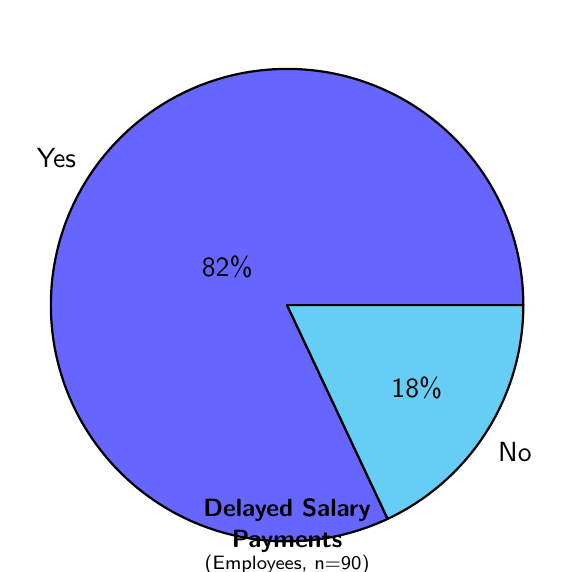
\begin{tikzpicture}
            \pie{82/Yes, 18/No}
            \node[font=\small\bfseries, text width=3cm, align=center] at (0,-2.8) {Delayed Salary Payments};
            \node[font=\scriptsize] at (0,-3.3) {(Employees, n=90)};
        \end{tikzpicture}
        \caption{}
        \label{fig:yesno_salary_doughnut}
    \end{subfigure}
    \begin{subfigure}{0.32\textwidth}
        \centering
        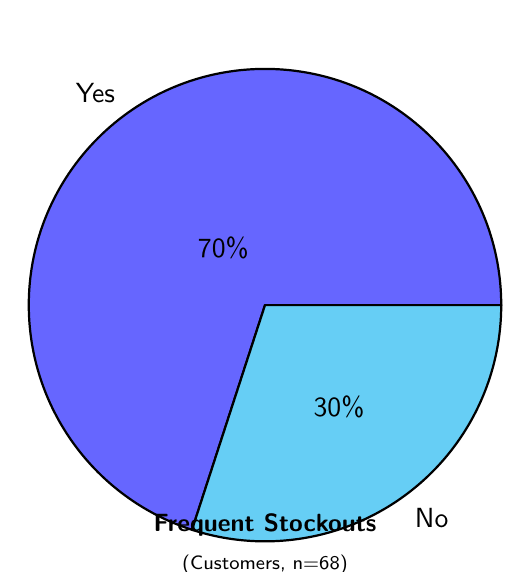
\begin{tikzpicture}
            \pie{70/Yes, 30/No}
            \node[font=\small\bfseries, text width=3cm, align=center] at (0,-2.8) {Frequent Stockouts};
            \node[font=\scriptsize] at (0,-3.3) {(Customers, n=68)};
        \end{tikzpicture}
        \caption{}
        \label{fig:yesno_stockouts_doughnut}
    \end{subfigure}
    \begin{subfigure}{0.32\textwidth}
        \centering
        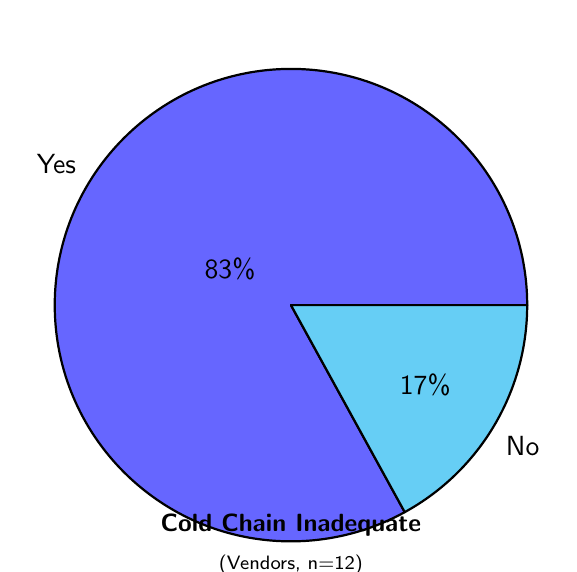
\begin{tikzpicture}
            \pie{83/Yes, 17/No}
            \node[font=\small\bfseries, text width=3.5cm, align=center] at (0,-2.8) {Cold Chain Inadequate};
            \node[font=\scriptsize] at (0,-3.3) {(Vendors, n=12)};
        \end{tikzpicture}
        \caption{}
        \label{fig:yesno_coldchain_doughnut}
    \end{subfigure}
    \caption{Doughnut Charts of Selected Yes/No Questionnaire Responses}
    \label{fig:yesno_doughnuts}
\end{figure}

\begin{figure}[H]
    \centering
    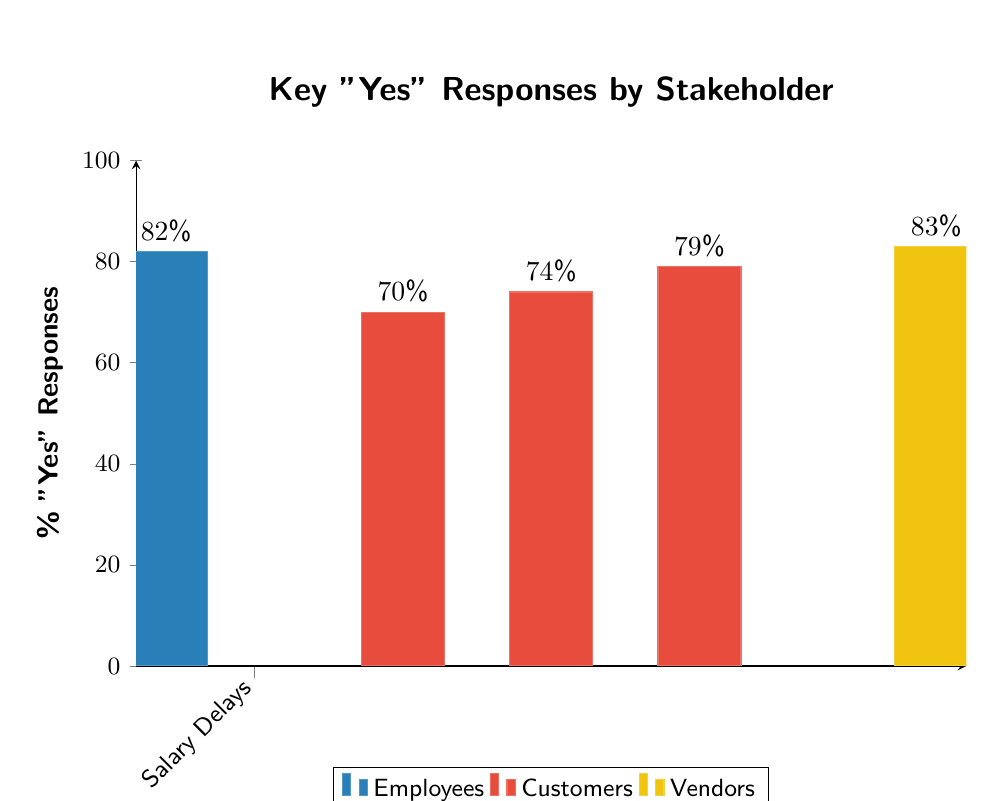
\begin{tikzpicture}
        \begin{axis}[
            ybar, % Use ybar instead of ybar stacked for this data structure
            bar width=30pt,
            width=\textwidth,
            height=8cm,
            enlarge x limits=0.2,
            ylabel={\% "Yes" Responses},
            symbolic x coords={Salary Delays, Stockouts, Delivery Delays, App Issues, Cold Chain Issues},
            xtick=data,
            xticklabel style={rotate=45, anchor=east, font=\small},
            ymin=0, ymax=100,
            ytick={0,20,40,60,80,100},
            nodes near coords={\pgfmathprintnumber{\pgfplotspointmeta}\%}, % Add value labels
            nodes near coords align={vertical},
            title={Key "Yes" Responses by Stakeholder},
        ]
        \addplot[fill=primary, draw=primary!80] coordinates {(Salary Delays, 82)};
        \addplot[fill=accent, draw=accent!80] coordinates {(Stockouts, 70) (Delivery Delays, 74) (App Issues, 79)};
        \addplot[fill=warning, draw=warning!80] coordinates {(Cold Chain Issues, 83)};
        \legend{Employees, Customers, Vendors}
        \end{axis}
    \end{tikzpicture}
    \caption{Bar Chart of Key "Yes" Responses}
    \label{fig:yesno_bar}
\end{figure}

\hrulefill

\textbf{Likert-Scale Questions Results}

The Likert-scale questions measure the perceived intensity of each problem. Radar charts provide a visual comparison of multiple factors for each group.

\begin{figure}[H]
    \centering
    % Helper macro for radar chart axes
    \newcommand{\radaraxis}[2]{
        \foreach \r in {1,2,3,4,5} {
            \draw[gray!30] (0,0) circle (0.4*\r);
            \node[font=\tiny] at (90:0.4*\r+0.15) {\r};
        }
        \foreach \angle/\label in {#1} {
            \draw[gray!50, thick] (0,0) -- (\angle:2.2);
            \node[font=\small, align=center] at (\angle:2.6) {\label};
        }
    }
    \begin{subfigure}{0.32\textwidth}
        \centering
        
\begin{tikzpicture}
            \begin{axis}[width=6cm, height=6cm, axis equal, axis lines=none, clip=false]
                \radaraxis{90/Financial, 162/HR, 234/Delivery, 306/Tech, 18/Inventory}{}
                \coordinate (A) at (90:{4.5*0.4});
                \coordinate (B) at (162:{4.6*0.4});
                \coordinate (C) at (234:{4.5*0.4});
                \coordinate (D) at (306:{4.3*0.4});
                \coordinate (E) at (18:{4.5*0.4});
                \fill[primary!30, opacity=0.7] (A)--(B)--(C)--(D)--(E)--cycle;
                \draw[primary, thick] (A)--(B)--(C)--(D)--(E)--cycle;
                \foreach \p in {A,B,C,D,E} {\fill[primary] (\p) circle (2pt);}
            \end{axis}
            \node[font=\bfseries] at (0,-3.5) {Employee Perceptions};
        \end{tikzpicture}
        \caption{}
    \end{subfigure}
    \begin{subfigure}{0.32\textwidth}
        \centering
        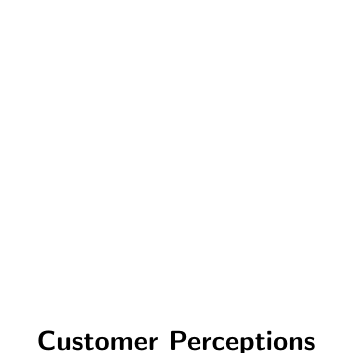
\begin{tikzpicture}
            \begin{axis}[width=6cm, height=6cm, axis equal, axis lines=none, clip=false]
                \radaraxis{45/Branding, 135/Stockouts, 225/Delays, 315/App Usability}{}
                \coordinate (A) at (45:{4.0*0.4});
                \coordinate (B) at (135:{4.2*0.4});
                \coordinate (C) at (225:{4.3*0.4});
                \coordinate (D) at (315:{4.5*0.4});
                \fill[accent!30, opacity=0.7] (A)--(B)--(C)--(D)--cycle;
                \draw[accent, thick] (A)--(B)--(C)--(D)--cycle;
                \foreach \p in {A,B,C,D} {\fill[accent] (\p) circle (2pt);}
            \end{axis}
            \node[font=\bfseries] at (0,-3.5) {Customer Perceptions};
        \end{tikzpicture}
        \caption{}
    \end{subfigure}
    \begin{subfigure}{0.32\textwidth}
        \centering
        \begin{tikzpicture}
            \begin{axis}[width=6cm, height=6cm, axis equal, axis lines=none, clip=false]
                \radaraxis{90/Payment, 270/Cold Chain}{}
                \coordinate (A) at (90:{4.5*0.4});
                \coordinate (B) at (270:{4.4*0.4});
                \fill[warning!30, opacity=0.7] (A)--(B)--(0,0)--cycle;
                \draw[warning, thick] (A)--(B);
                \foreach \p in {A,B} {\fill[warning] (\p) circle (2pt);}
            \end{axis}
            \node[font=\bfseries] at (0,-3.5) {Vendor Perceptions};
        \end{tikzpicture}
        \caption{}
    \end{subfigure}
    \caption{Radar Charts of Likert-Scale Responses by Stakeholder (Scale 1-5)}
    \label{fig:likert_radars}
\end{figure}

\begin{figure}[H]
    \centering
    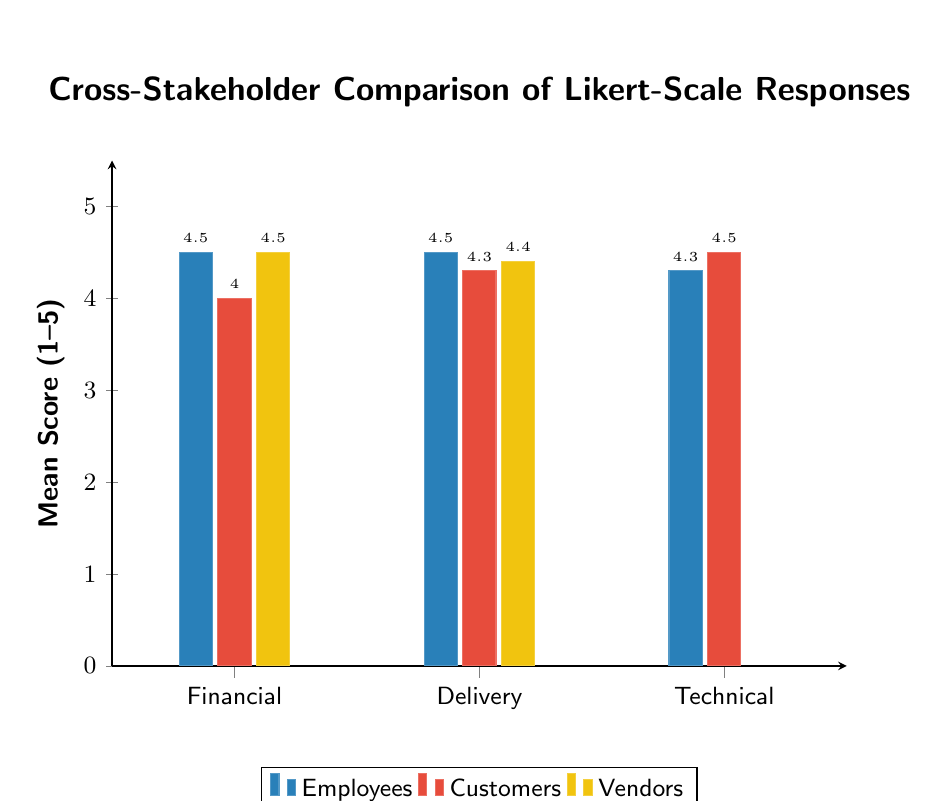
\begin{tikzpicture}
        \begin{axis}[
            ybar,
            bar width=12pt,
            width=0.9\textwidth,
            height=8cm,
            enlarge x limits=0.25,
            ylabel={Mean Score (1–5)},
            symbolic x coords={Financial, Delivery, Technical},
            xtick=data,
            ymin=0, ymax=5.5,
            nodes near coords,
            nodes near coords style={font=\tiny, /pgf/number format/fixed, /pgf/number format/precision=1},
            title={Cross-Stakeholder Comparison of Likert-Scale Responses},
            legend style={at={(0.5, -0.2)}, anchor=north, legend columns=3}
        ]
        \addplot[fill=primary, draw=primary!80] coordinates {(Financial, 4.5) (Delivery, 4.5) (Technical, 4.3)};
        \addplot[fill=accent, draw=accent!80] coordinates {(Financial, 4.0) (Delivery, 4.3) (Technical, 4.5)};
        \addplot[fill=warning, draw=warning!80] coordinates {(Financial, 4.5) (Delivery, 4.4)};
        \legend{Employees, Customers, Vendors}
        \end{axis}
    \end{tikzpicture}
    \caption{Grouped Bar Chart of Key Likert-Scale Responses}
    \label{fig:likert_grouped_bar}
\end{figure}

\hrulefill

\textbf{Ranking Questions Results}

Ranking questions forced stakeholders to prioritize their most significant concerns, providing a clear hierarchy of issues.

\begin{figure}[H]
    \centering
    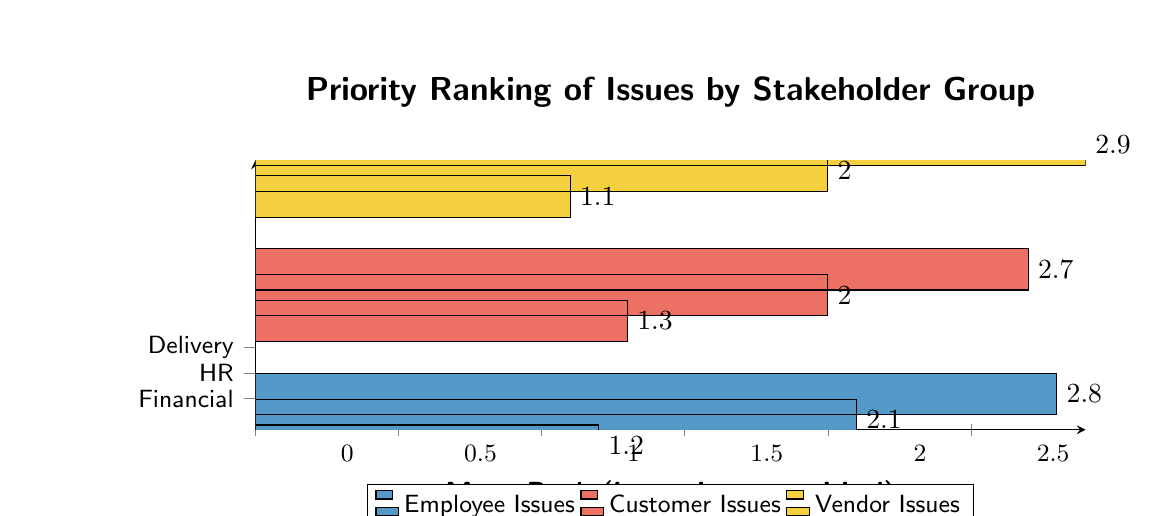
\begin{tikzpicture}
        \begin{axis}[
            xbar,
            width=\textwidth,
            height=5cm,
            bar width=15pt,
            xlabel={Mean Rank (Lower is more critical)},
            symbolic y coords={Financial, HR, Delivery, Delays, Stockouts, App, Payments, Cold Chain, Contracts},
            ytick=data,
            enlarge y limits=0.15,
            nodes near coords,
            nodes near coords align={horizontal},
            title={Priority Ranking of Issues by Stakeholder Group},
            ticklabel style={align=right, text width=2.5cm},
            xmin=0
        ]
        \addplot[fill=primary!80] coordinates {(1.2,Financial) (2.1,HR) (2.8,Delivery)};
        \addplot[fill=accent!80] coordinates {(1.3,Delays) (2.0,Stockouts) (2.7,App)};
        \addplot[fill=warning!80] coordinates {(1.1,Payments) (2.0,Cold Chain) (2.9,Contracts)};
        \legend{Employee Issues, Customer Issues, Vendor Issues}
        \end{axis}
    \end{tikzpicture}
    \caption{Combined Horizontal Bar Chart of Ranking Responses}
    \label{fig:ranking_combined}
\end{figure}

\hrulefill

\textbf{Summary Tables}

The following tables summarize the raw data from the questionnaire, highlighting the most critical findings for each question type.

% Independent pie charts for Yes/No Questionnaire Responses
{\large\bfseries Key Yes/No Questionnaire Results}
\vspace{0.7em}

% Delayed salary payments (Employees)
\begin{center}
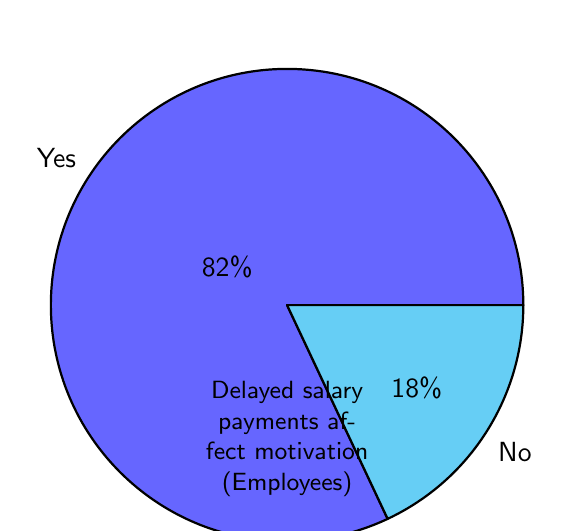
\begin{tikzpicture}
    \pie{82/Yes, 18/No}
    \node[font=\small, text width=3.2cm, align=center] at (0,-1.7) {Delayed salary payments affect motivation\\(Employees)};
\end{tikzpicture}
\end{center}
\vspace{0.5em}

% Frequent stockouts (Customers)
\begin{center}
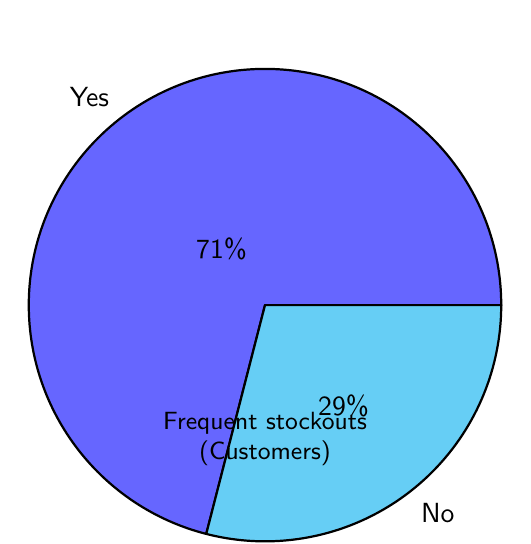
\begin{tikzpicture}
    \pie{71/Yes, 29/No}
    \node[font=\small, text width=3.2cm, align=center] at (0,-1.7) {Frequent stockouts\\(Customers)};
\end{tikzpicture}
\end{center}
\vspace{0.5em}

% Frequent delivery delays (Customers)
\begin{center}
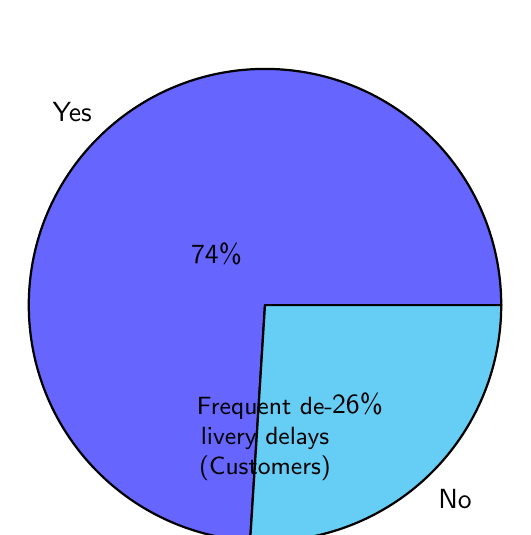
\begin{tikzpicture}
    \pie{74/Yes, 26/No}
    \node[font=\small, text width=3.2cm, align=center] at (0,-1.7) {Frequent delivery delays\\(Customers)};
\end{tikzpicture}
\end{center}
\vspace{0.5em}

% Cold chain inadequate (Vendors)
\begin{center}
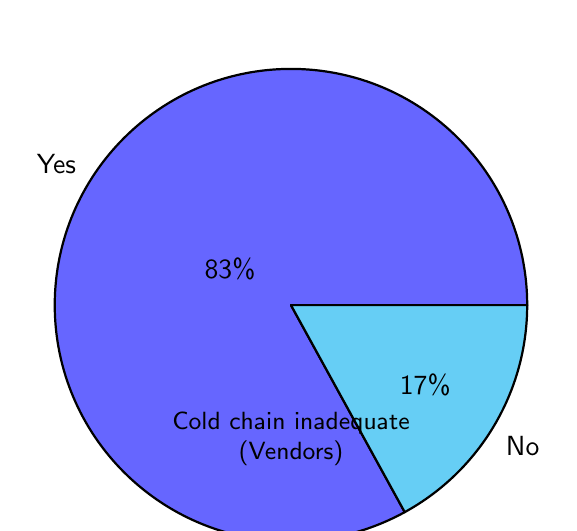
\begin{tikzpicture}
    \pie{83/Yes, 17/No}
    \node[font=\small, text width=3.2cm, align=center] at (0,-1.7) {Cold chain inadequate\\(Vendors)};
\end{tikzpicture}
\end{center}
\vspace{0.5em}

% App user-friendly and fast (Customers)
\begin{center}
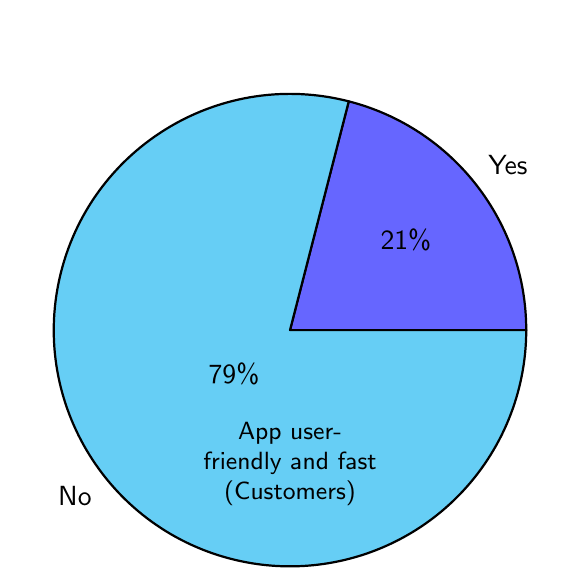
\begin{tikzpicture}
    \pie{21/Yes, 79/No}
    \node[font=\small, text width=3.2cm, align=center] at (0,-1.7) {App user-friendly and fast\\(Customers)};
\end{tikzpicture}
\end{center}

\begin{table}[H]
    \centering
    \caption{Summary of Likert-Scale Questionnaire Responses (1-5 Scale)}
    \label{tab:likert_summary}
    \renewcommand{\arraystretch}{1.3}
    \begin{tabular}{l l S[table-format=1.1] l S[table-format=3.1, table-space-text-post=\%]}
        \toprule
        \rowcolor{gray!15} \textbf{Question} & \textbf{Group} & {\textbf{Mean}} & {\textbf{(SD)}} & {\textbf{\% Rated 4 or 5}} \\
        \midrule
        \rowcolor{primary!10} Financial constraints limit growth & Employees & 4.5 & (0.6) & 91.1\% \\
        \rowcolor{accent!10} Frequent stockouts reduce satisfaction & Customers & 4.2 & (0.7) & 79.4\% \\
        Delivery delays reduce satisfaction & Customers & 4.3 & (0.7) & 83.8\% \\
        \rowcolor{warning!10} Delayed payments impact vendor business & Vendors & 4.5 & (0.5) & 91.7\% \\
        \bottomrule
    \end{tabular}
\end{table}

\begin{table}[H]
    \centering
    \caption{Summary of Ranking Questionnaire Responses (Top 3)}
    \label{tab:ranking_summary}
    \renewcommand{\arraystretch}{1.3}
    \begin{tabular}{p{5cm} l l}
        \toprule
        \rowcolor{gray!15} \textbf{Question Area} & \textbf{Group} & \textbf{Mean Rank (Top 3)} \\
        \midrule
        \rowcolor{primary!10} \multirow{3}{*}{Issues impacting work} & \multirow{3}{*}{Employees} & 1. Financial constraints (1.2) \\
        & & 2. HR inefficiencies (2.1) \\
        & & 3. Delivery operations (2.8) \\
        \midrule
        \rowcolor{accent!10} \multirow{3}{*}{Factors affecting satisfaction} & \multirow{3}{*}{Customers} & 1. Delivery delays (1.3) \\
        & & 2. Stockouts (2.0) \\
        & & 3. App performance (2.7) \\
        \midrule
        \rowcolor{warning!10} \multirow{3}{*}{Barriers to vendor reliability} & \multirow{3}{*}{Vendors} & 1. Payment delays (1.1) \\
        & & 2. Cold chain issues (2.0) \\
        & & 3. Lack of contracts (2.9) \\
        \bottomrule
    \end{tabular}
\end{table}

\hrulefill

\subsubsection*{Summary of Key Findings}
The analytical results, supported by diverse visualizations and summary tables, provide a comprehensive and quantitative assessment of Chaldal's core challenges. The following key findings are drawn from the questionnaire data and stakeholder feedback:

\begin{itemize}
    \item \textbf{Employees:} Financial constraints are the most pressing concern, with 82\% reporting that delayed salary payments negatively affect motivation and 91\% rating financial limitations as a major barrier to growth (Mean Likert: 4.5). HR inefficiencies are also prominent, with 78\% indicating that manual HR processes cause scheduling errors and 85\% agreeing that lack of transparency affects morale. Employees consistently ranked financial constraints (mean rank 1.2) and HR issues (mean rank 2.1) as the top factors impacting their work experience and retention.
    \item \textbf{Customers:} Operational failures dominate customer concerns. Delivery delays are reported by 74\% of respondents, and 71\% experience frequent stockouts of fresh produce. On the Likert scale, delivery delays (mean: 4.3) and stockouts (mean: 4.2) are rated as severe issues, with 84\% and 79\% respectively scoring them at 4 or 5. App usability is also problematic, with only 21\% finding the mobile app user-friendly and fast, and 79\% reporting performance issues that lead to lost sales. Customers ranked delivery delays (mean rank 1.3), stockouts (2.0), and app performance (2.7) as the most impactful factors affecting satisfaction.
    \item \textbf{Vendors:} Payment delays and cold chain limitations are critical pain points. 83\% of vendors view Chaldal’s cold chain infrastructure as inadequate, and 92\% rate delayed payments as a major negative impact on their business (Mean Likert: 4.5). Vendors ranked payment delays (mean rank 1.1) and cold chain issues (2.0) as the top barriers to reliability, with lack of standardized contracts and poor forecasting also contributing to supply chain challenges.
\end{itemize}

Overall, the data reveals a strong consensus across all stakeholder groups: financial instability, operational inefficiencies, and technical shortcomings are deeply interconnected and have a measurable negative impact on Chaldal’s business performance, employee morale, customer satisfaction, and vendor relationships. These findings provide a robust, data-driven foundation for developing targeted strategic recommendations in the next chapter.




\paragraph{DFD of Existing System}

This section presents Data Flow Diagrams (DFDs) illustrating the structure and information flow of Chaldal's current system. The first diagram provides an overview of the main system, while the subsequent five diagrams detail the subsystems corresponding to the five core problem areas identified in the analysis.

\subparagraph{Main DFD: Overall System}

This diagram provides a high-level overview of the entire Chaldal system, breaking down the central process into its major subsystems. It illustrates the primary external entities and the main data flows between them and the core processes.
\begin{figure}
    \centering
    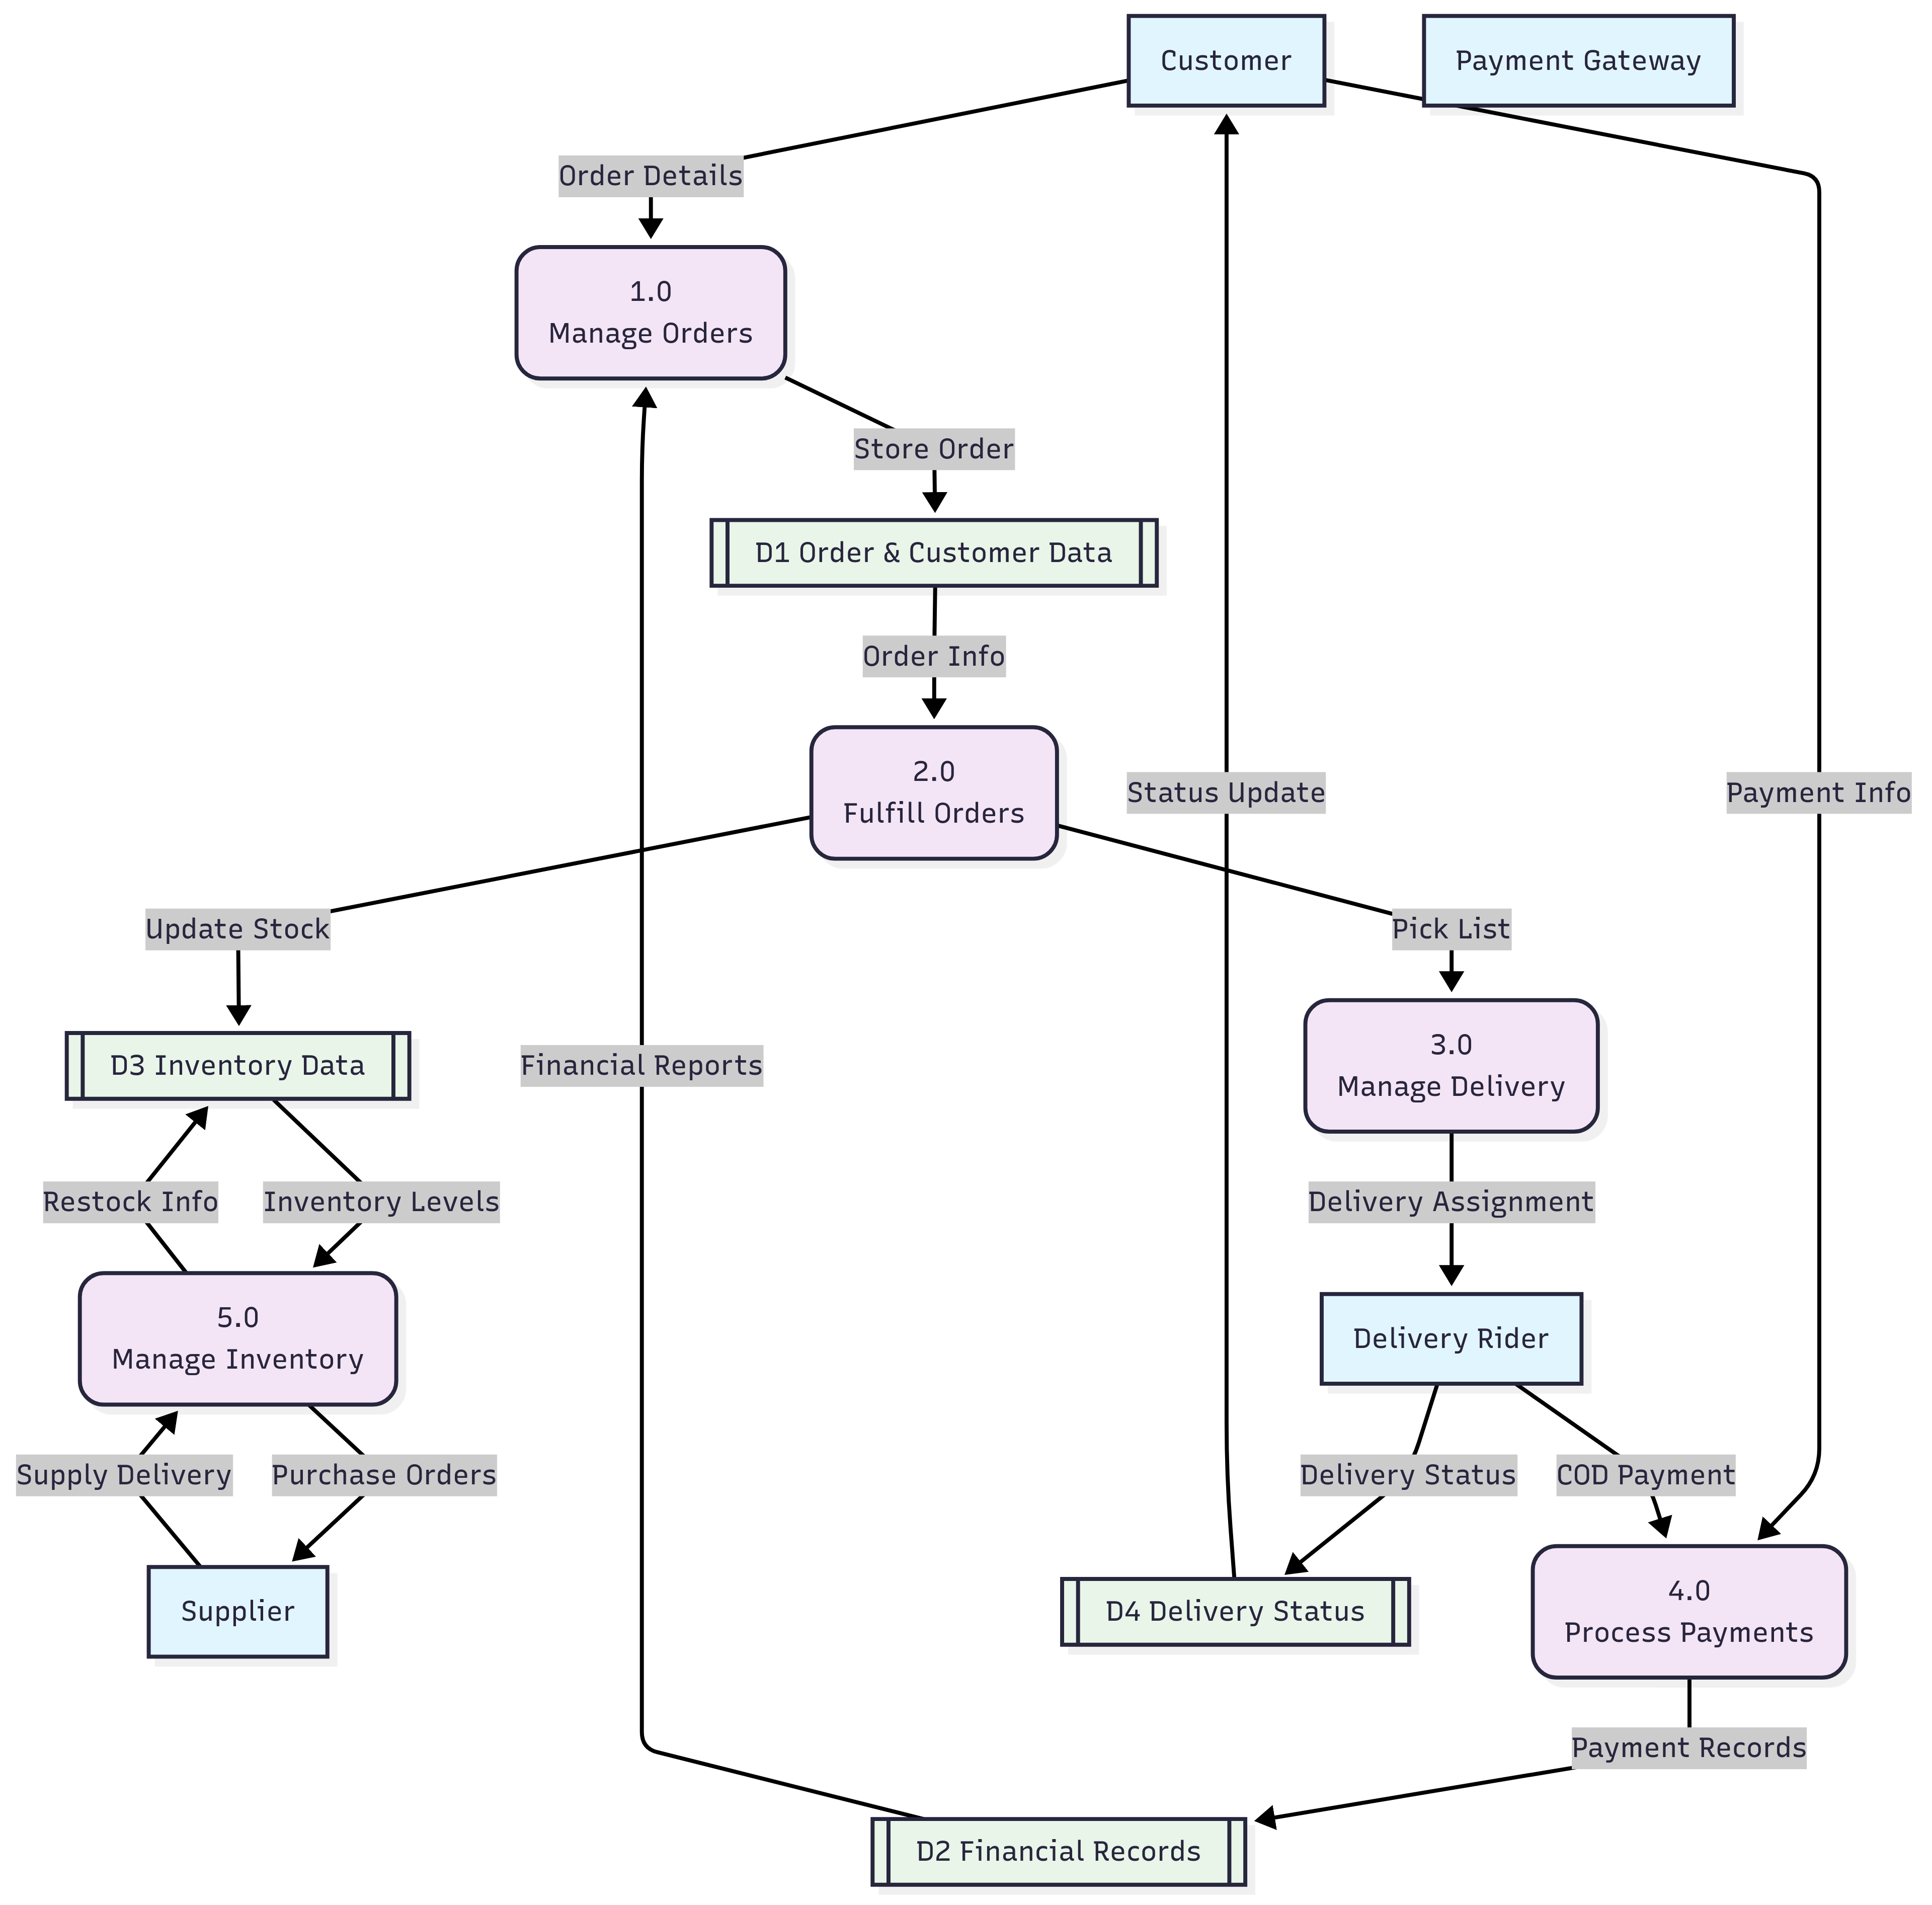
\includegraphics[width=1.0\textwidth]{l0_dfd_mermaid.png}
    \caption{Main DFD of Chaldal System Overview}
    \label{fig:dfd_main}
\end{figure}
\underline{\textit{DESCRIPTION:}} This Level 0 Data Flow Diagram provides a comprehensive overview of Chaldal's e-commerce and logistics ecosystem. The diagram illustrates how the five core processes interact to manage the complete order fulfillment cycle. The Customer external entity initiates the workflow by providing Order Details to the 1.0 Manage Orders process, which stores this information in the D1 Order \& Customer Data store. The 2.0 Fulfill Orders process retrieves order information and generates pick lists for warehouse operations, then passes fulfillment data to 3.0 Manage Delivery. This process coordinates with the Delivery Rider external entity for order dispatch and tracks delivery status in D4 Delivery Status. The 4.0 Process Payments process handles both upfront payments and COD collections, maintaining financial records in D2 Financial Records. Finally, 5.0 Manage Inventory monitors stock levels in D3 Inventory Data and generates purchase orders to Suppliers to maintain adequate inventory. This diagram effectively shows the integrated nature of Chaldal's operations, from order placement through delivery completion.


\paragraph{DFD for Problem 01: Lack of Profitability and Funding Constraints}
\hfill \break
This DFD illustrates the negative feedback loop where high operational costs, driven by an over-engineered infrastructure, lead to financial strain and an inability to invest in growth.
\begin{figure}[H]
    \centering
    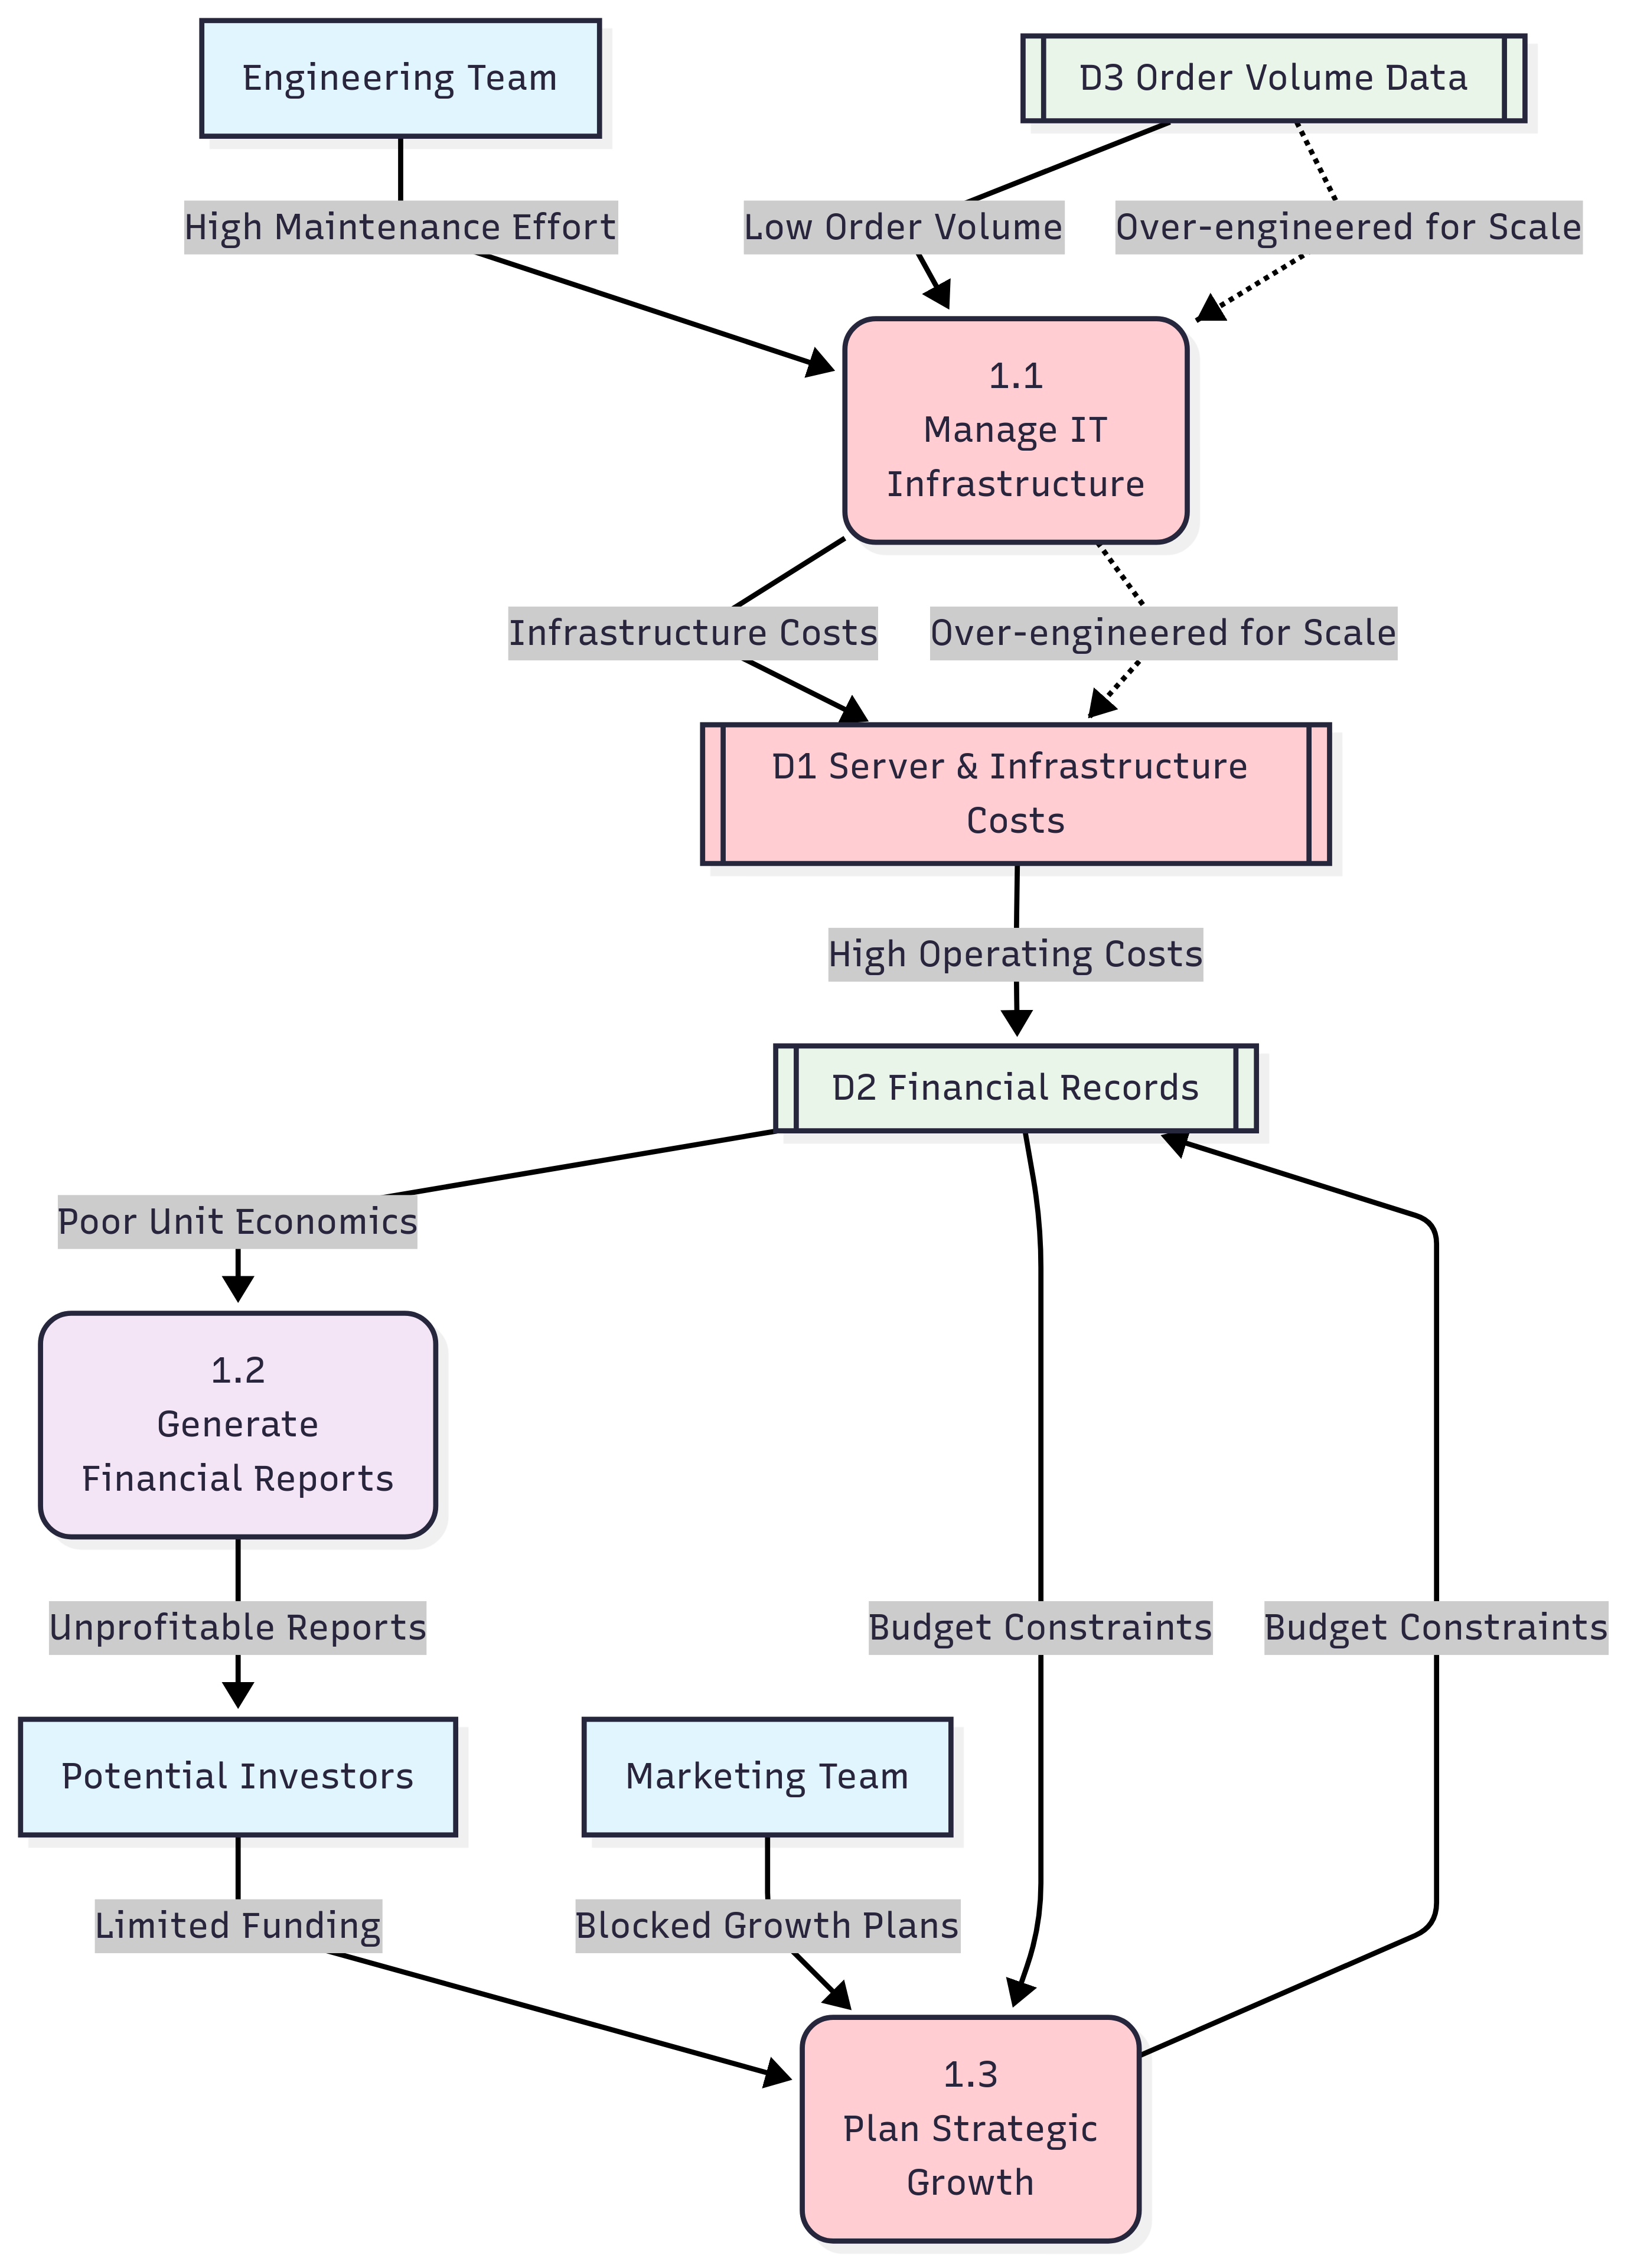
\includegraphics[width=.8\textwidth]{p1_dfd_mermaid.png}
    \caption{DFD of Financial Constraints Subsystem}
    \label{fig:dfd_financial}
\end{figure}
\underline{\textit{DESCRIPTION:}} This DFD illustrates the critical financial sustainability problem within Chaldal's system. The Engineering Team continuously provides high maintenance effort to the 1.1 Manage IT Infrastructure process, which is over-engineered relative to the current Low Order Volume from D3 Order Volume Data. This misalignment generates excessive Infrastructure Costs stored in D1 Server \& Infrastructure Costs, leading to High Operating Costs that flow into D2 Financial Records. The 1.2 Generate Financial Reports process produces unfavorable unit economics that deter Potential Investors, resulting in limited funding availability. This creates a damaging cycle where the 1.3 Plan Strategic Growth process cannot access adequate resources, effectively blocking growth initiatives for the Marketing Team. The dashed lines indicate constrained or blocked data flows, highlighting how the over-engineered infrastructure acts as a financial drain that prevents strategic investments in expansion, branding, and operational improvements essential for achieving profitability.

\paragraph{DFD for Problem 02: Supply Chain Inefficiencies and Product Sourcing Challenges}
\hfill \break
This DFD models the unreliable and costly procurement process that negatively impacts inventory, product quality, and customer trust.
\begin{figure}[H]
    \centering
    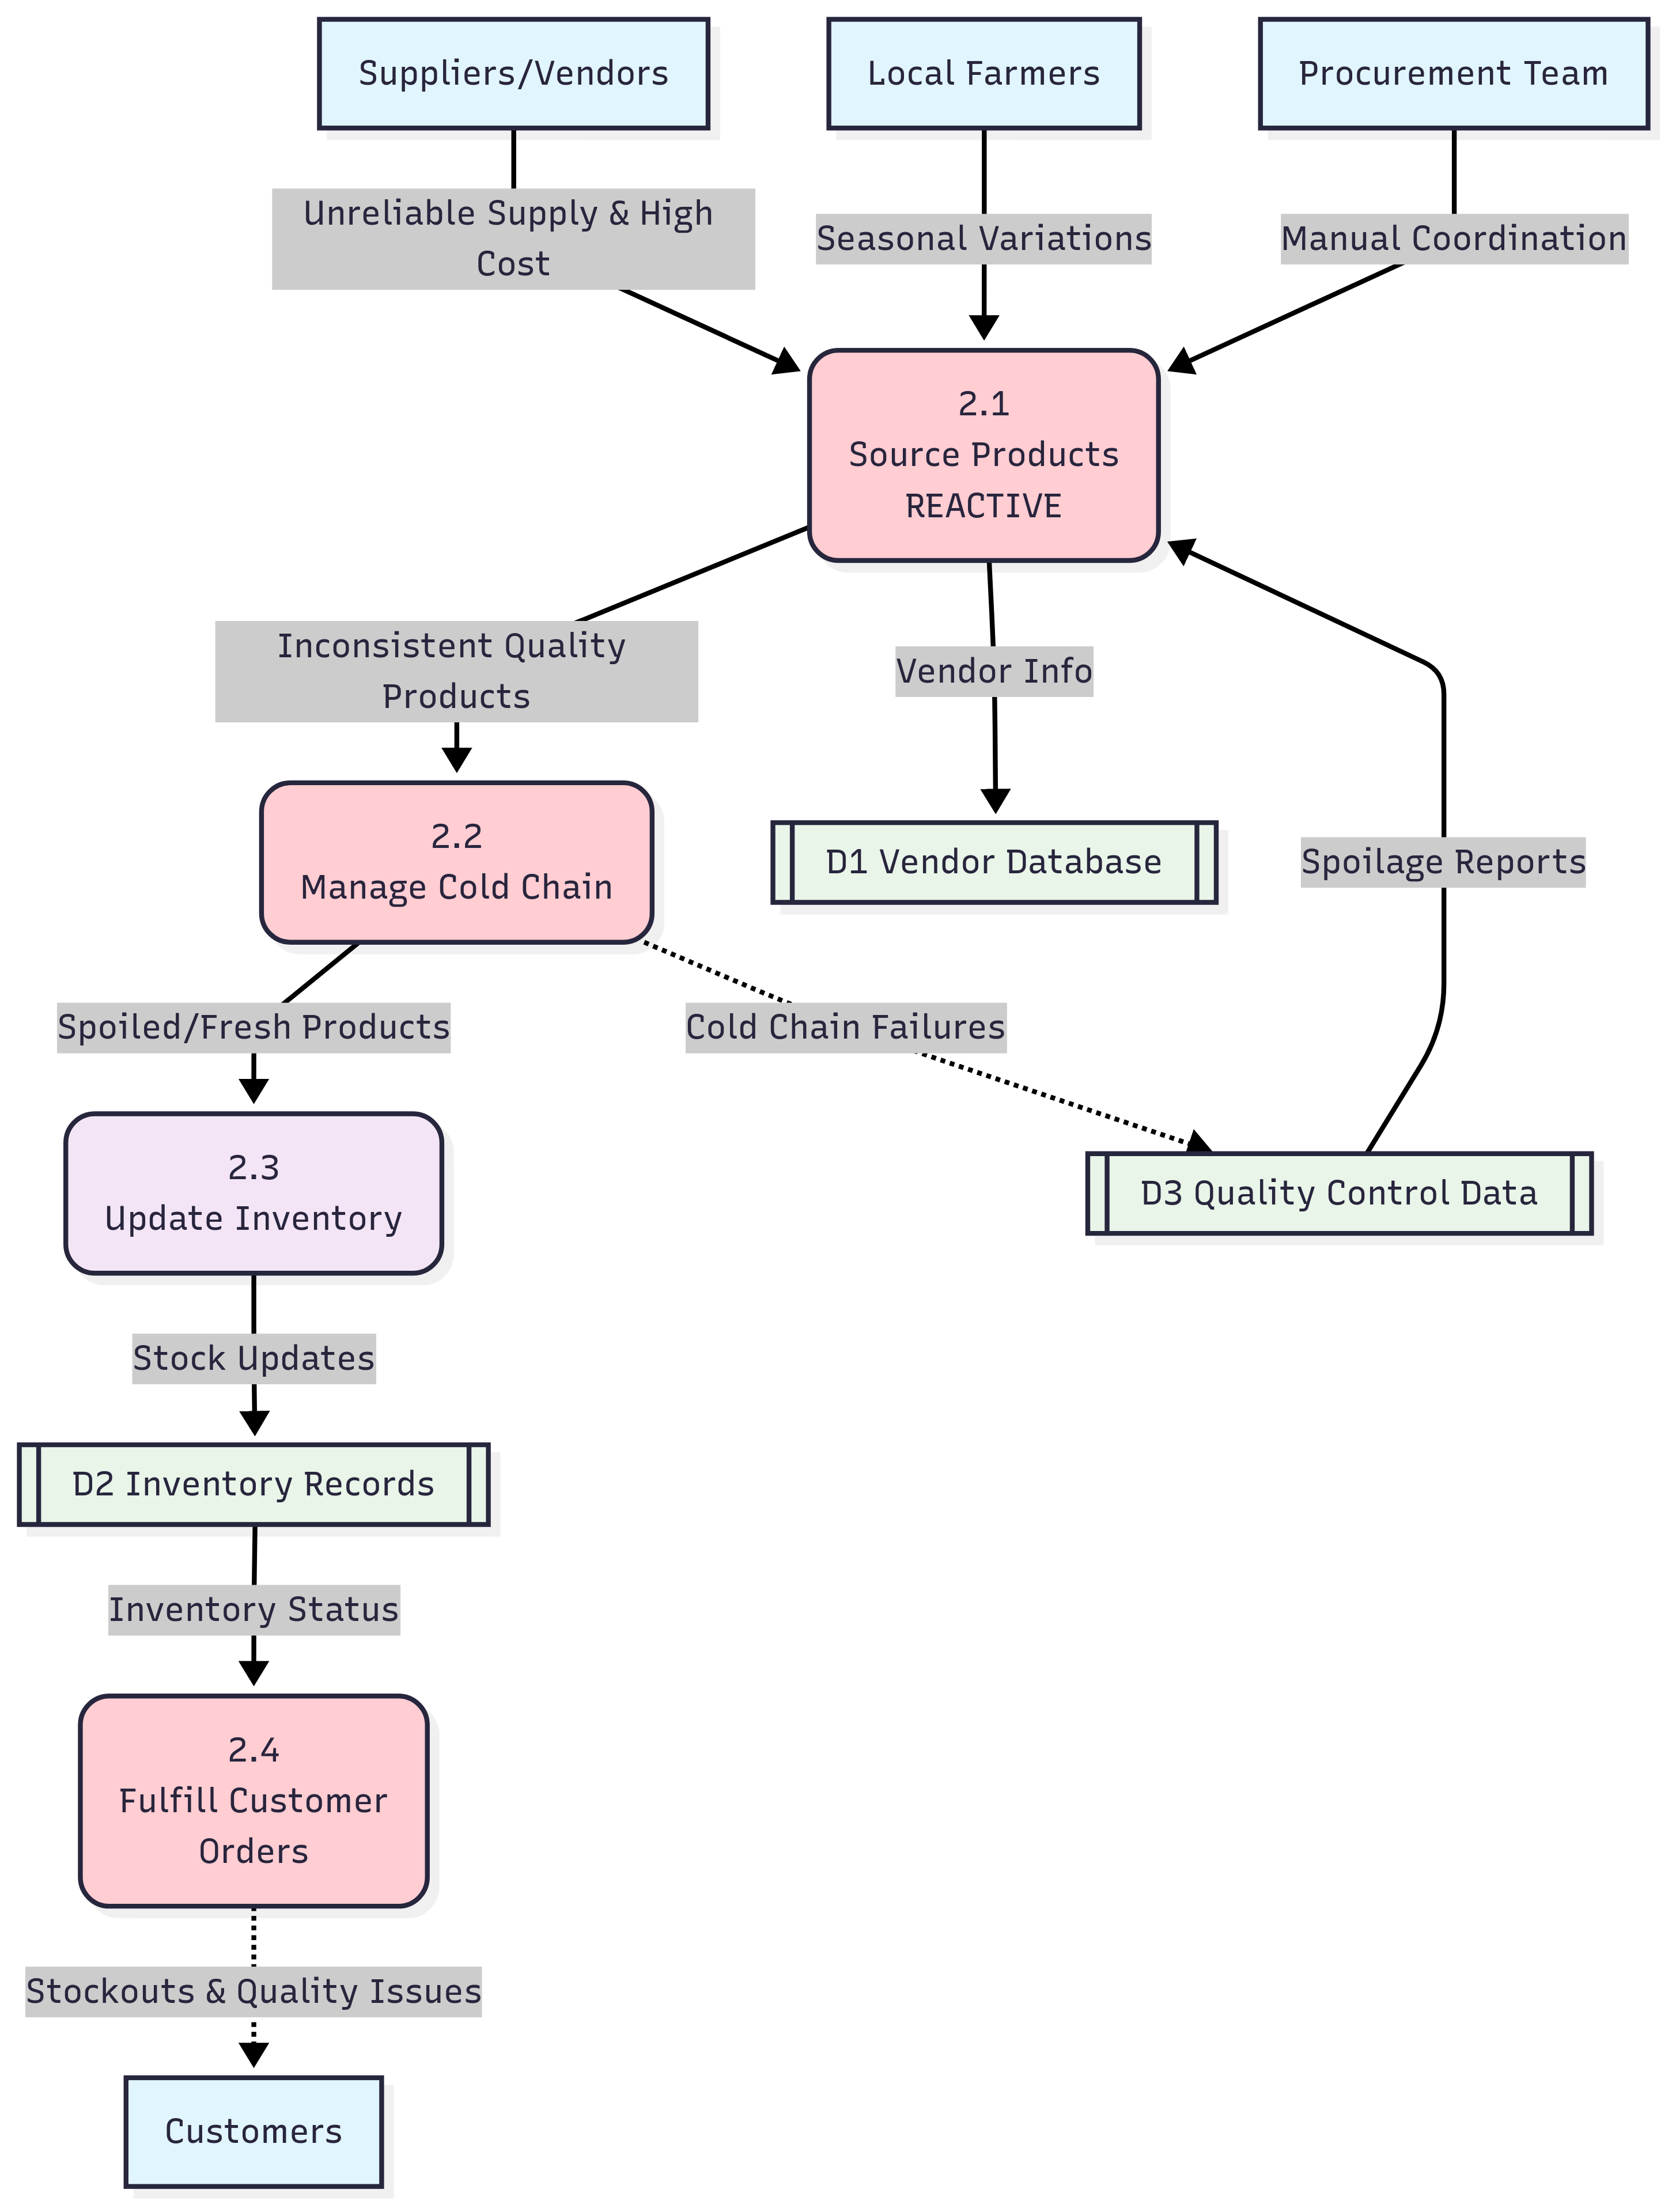
\includegraphics[width=.75\textwidth]{p2_dfd_mermaid.png}
    \caption{DFD of Supply Chain and Procurement Subsystem}
    \label{fig:dfd_supplychain}
\end{figure}
\underline{\textit{DESCRIPTION:}} This DFD depicts the systematic failures within Chaldal's supply chain management. Suppliers/Vendors and Local Farmers provide unreliable supply with high costs and seasonal variations to the 2.1 Source Products process, which is labeled as "REACTIVE" to emphasize the lack of proactive vendor management. The Procurement Team relies on manual coordination, leading to inefficiencies. The sourcing process feeds inconsistent quality products into the 2.2 Manage Cold Chain process, where inadequate cold chain infrastructure causes spoilage, creating failures that are recorded in D3 Quality Control Data. The 2.3 Update Inventory process receives both spoiled and fresh products, leading to inaccurate stock levels in D2 Inventory Records. When the 2.4 Fulfill Customer Orders process attempts to fulfill orders, it encounters stockouts and quality issues, resulting in incomplete or poor-quality deliveries to Customers. The dashed lines indicate problematic data flows, showing how initial sourcing inefficiencies cascade through the entire supply chain, ultimately degrading customer satisfaction and eroding brand trust.

\paragraph{DFD for Problem 03: Ineffective Customer Representative \& Delivery Operations}
\hfill \break
This DFD shows the operational risks and service inconsistencies stemming from the reliance on part-time delivery staff and Cash on Delivery (COD).
\begin{figure}[H]
    \centering
    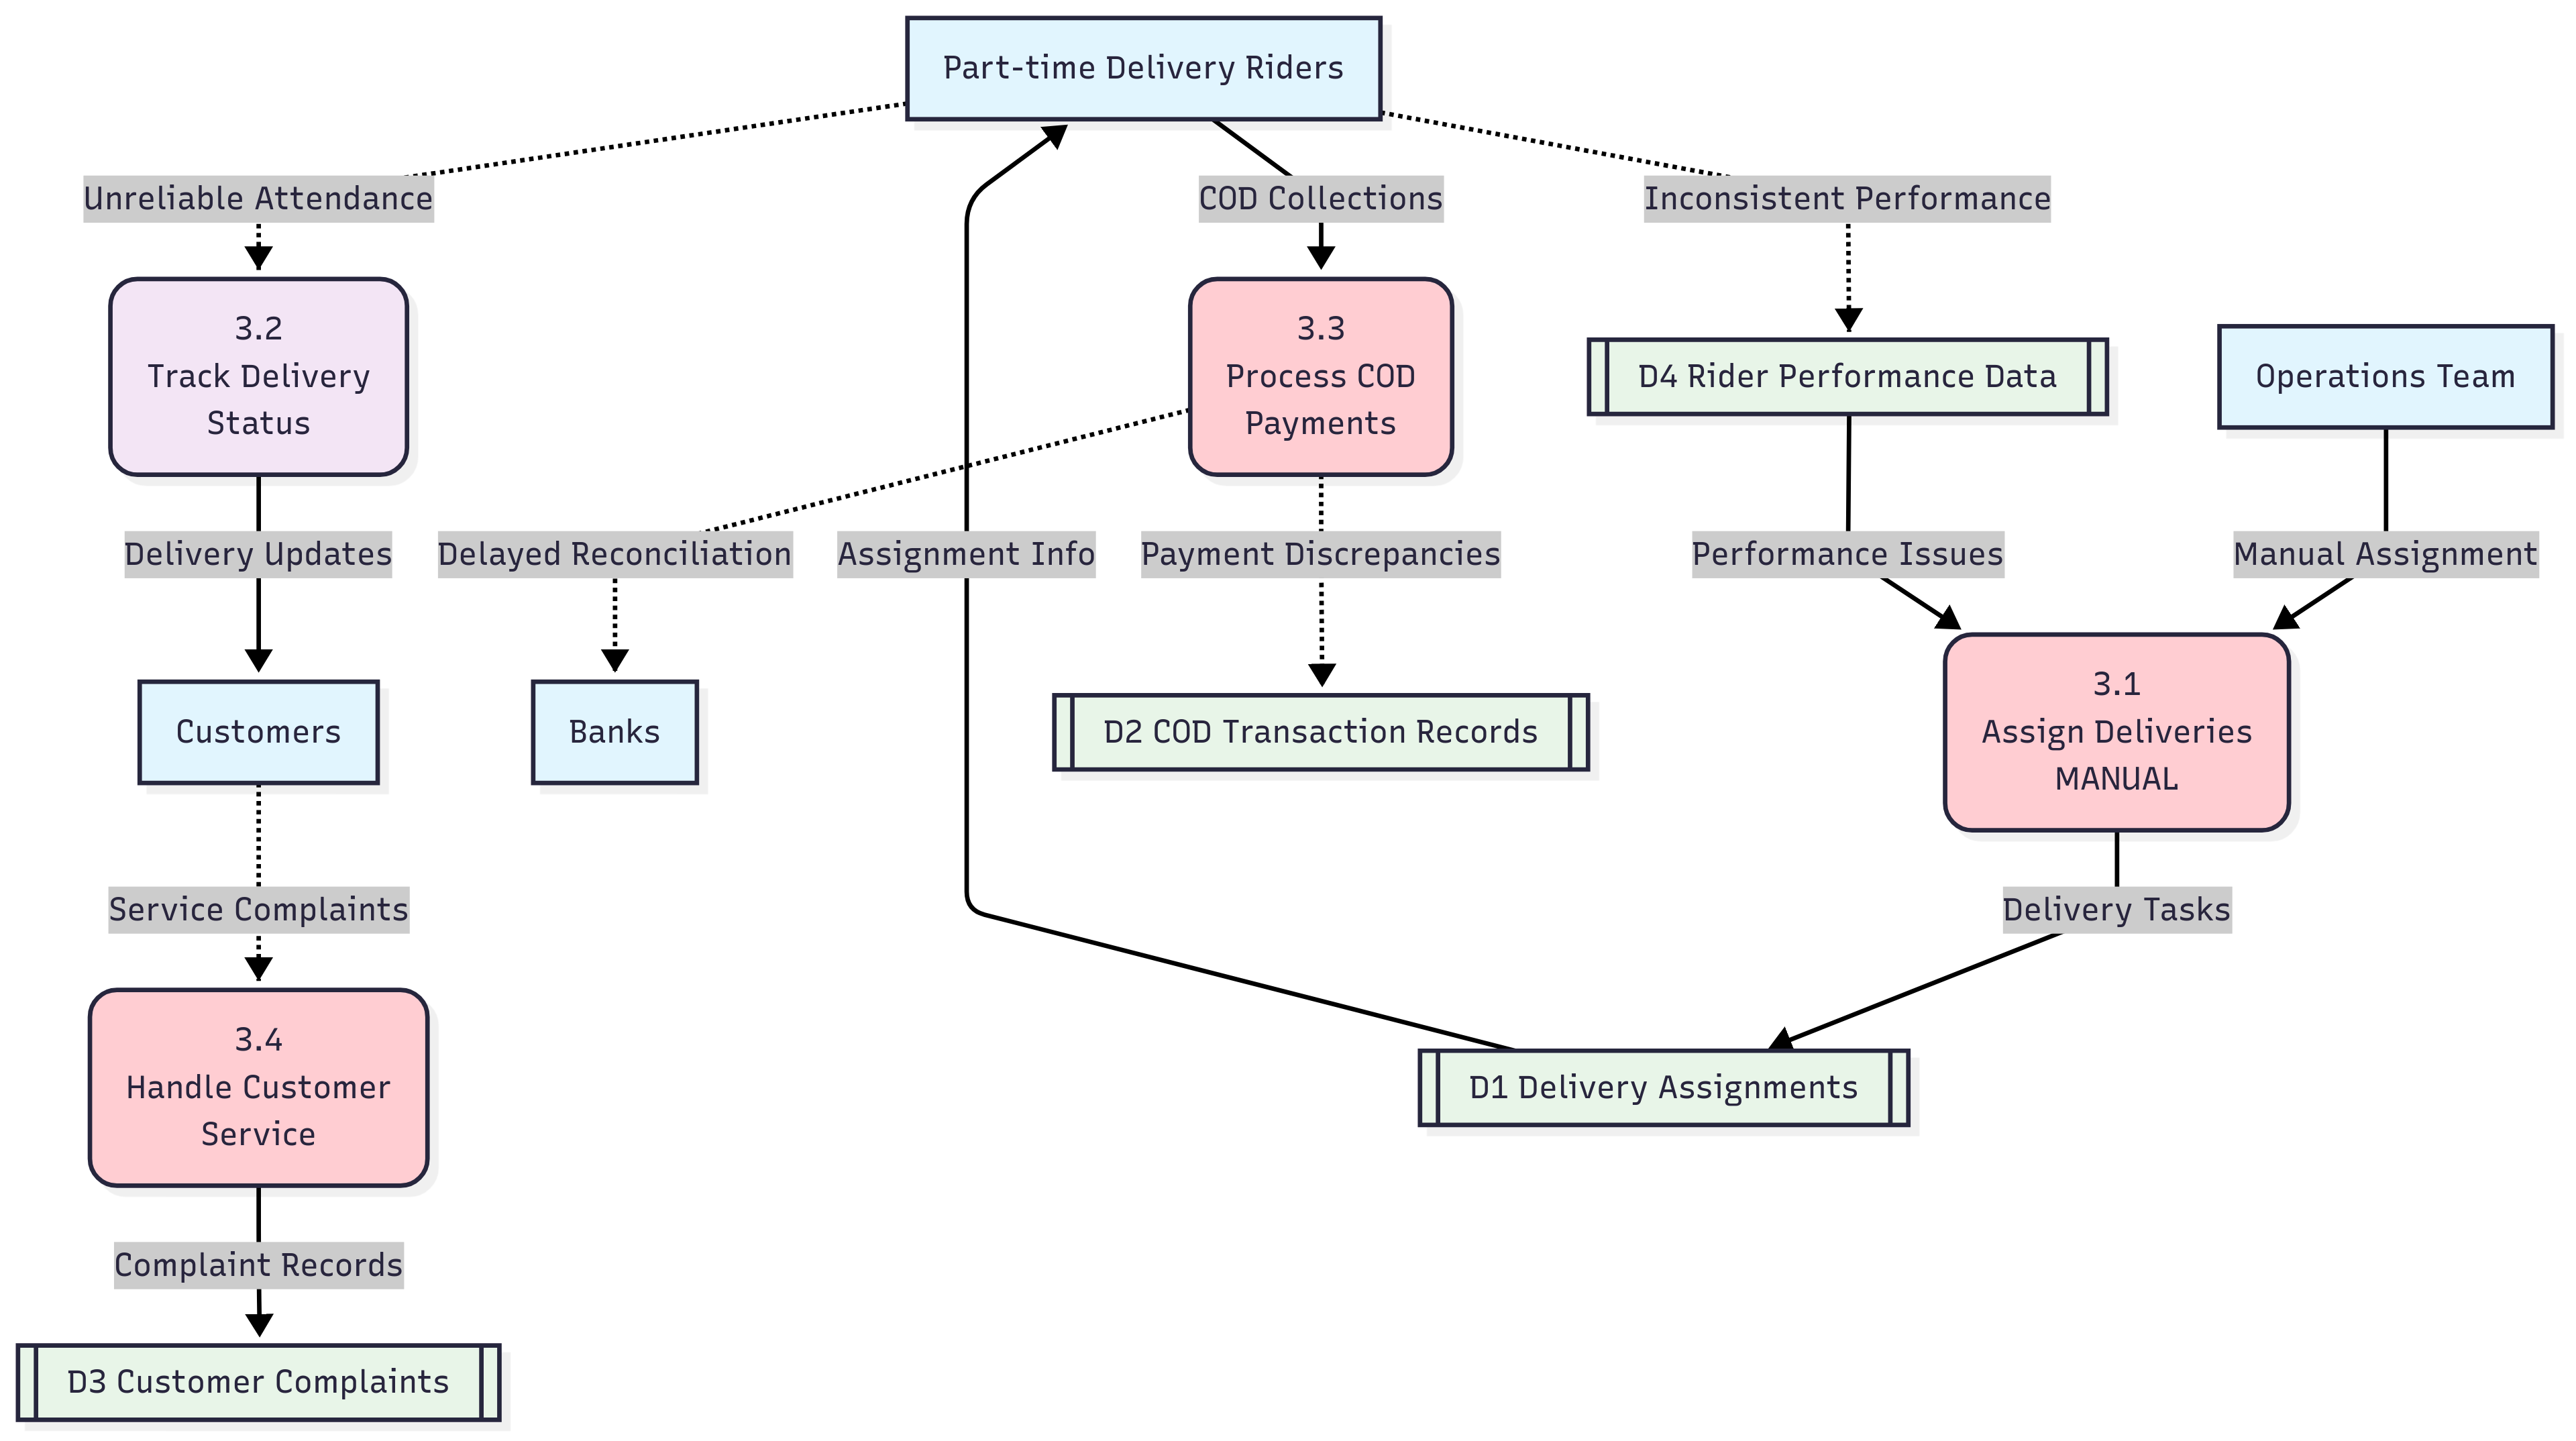
\includegraphics[width=1.0\textwidth]{p3_dfd_mermaid.png}
    \caption{DFD of Delivery Operations Subsystem}
    \label{fig:dfd_delivery}
\end{figure}
\underline{\textit{DESCRIPTION:}} This DFD highlights the operational vulnerabilities in Chaldal's delivery system. The Operations Team manually assigns deliveries through the 3.1 Assign Deliveries process (labeled "MANUAL"), creating inefficiencies in the D1 Delivery Assignments data store. Part-time Delivery Riders receive assignment information but exhibit unreliable attendance patterns that affect the 3.2 Track Delivery Status process. The riders handle COD collections through the 3.3 Process COD Payments process, which generates payment discrepancies stored in D2 COD Transaction Records and causes delayed reconciliation with Banks. The 3.4 Handle Customer Service process receives service complaints from Customers due to inconsistent delivery performance, storing these issues in D3 Customer Complaints. Inconsistent rider performance data in D4 Rider Performance Data creates a feedback loop that further complicates the assignment process. The dashed lines represent problematic data flows, illustrating how the reliance on part-time staff and manual processes creates a cascade of operational inefficiencies, financial risks from COD mishandling, and declining customer satisfaction.

\paragraph{DFD for Problem 04: Operational and HR Process Inefficiencies}
\hfill \break
This DFD illustrates the bottleneck and lack of transparency caused by manual HR and scheduling processes.
\begin{figure}[H]
    \centering
    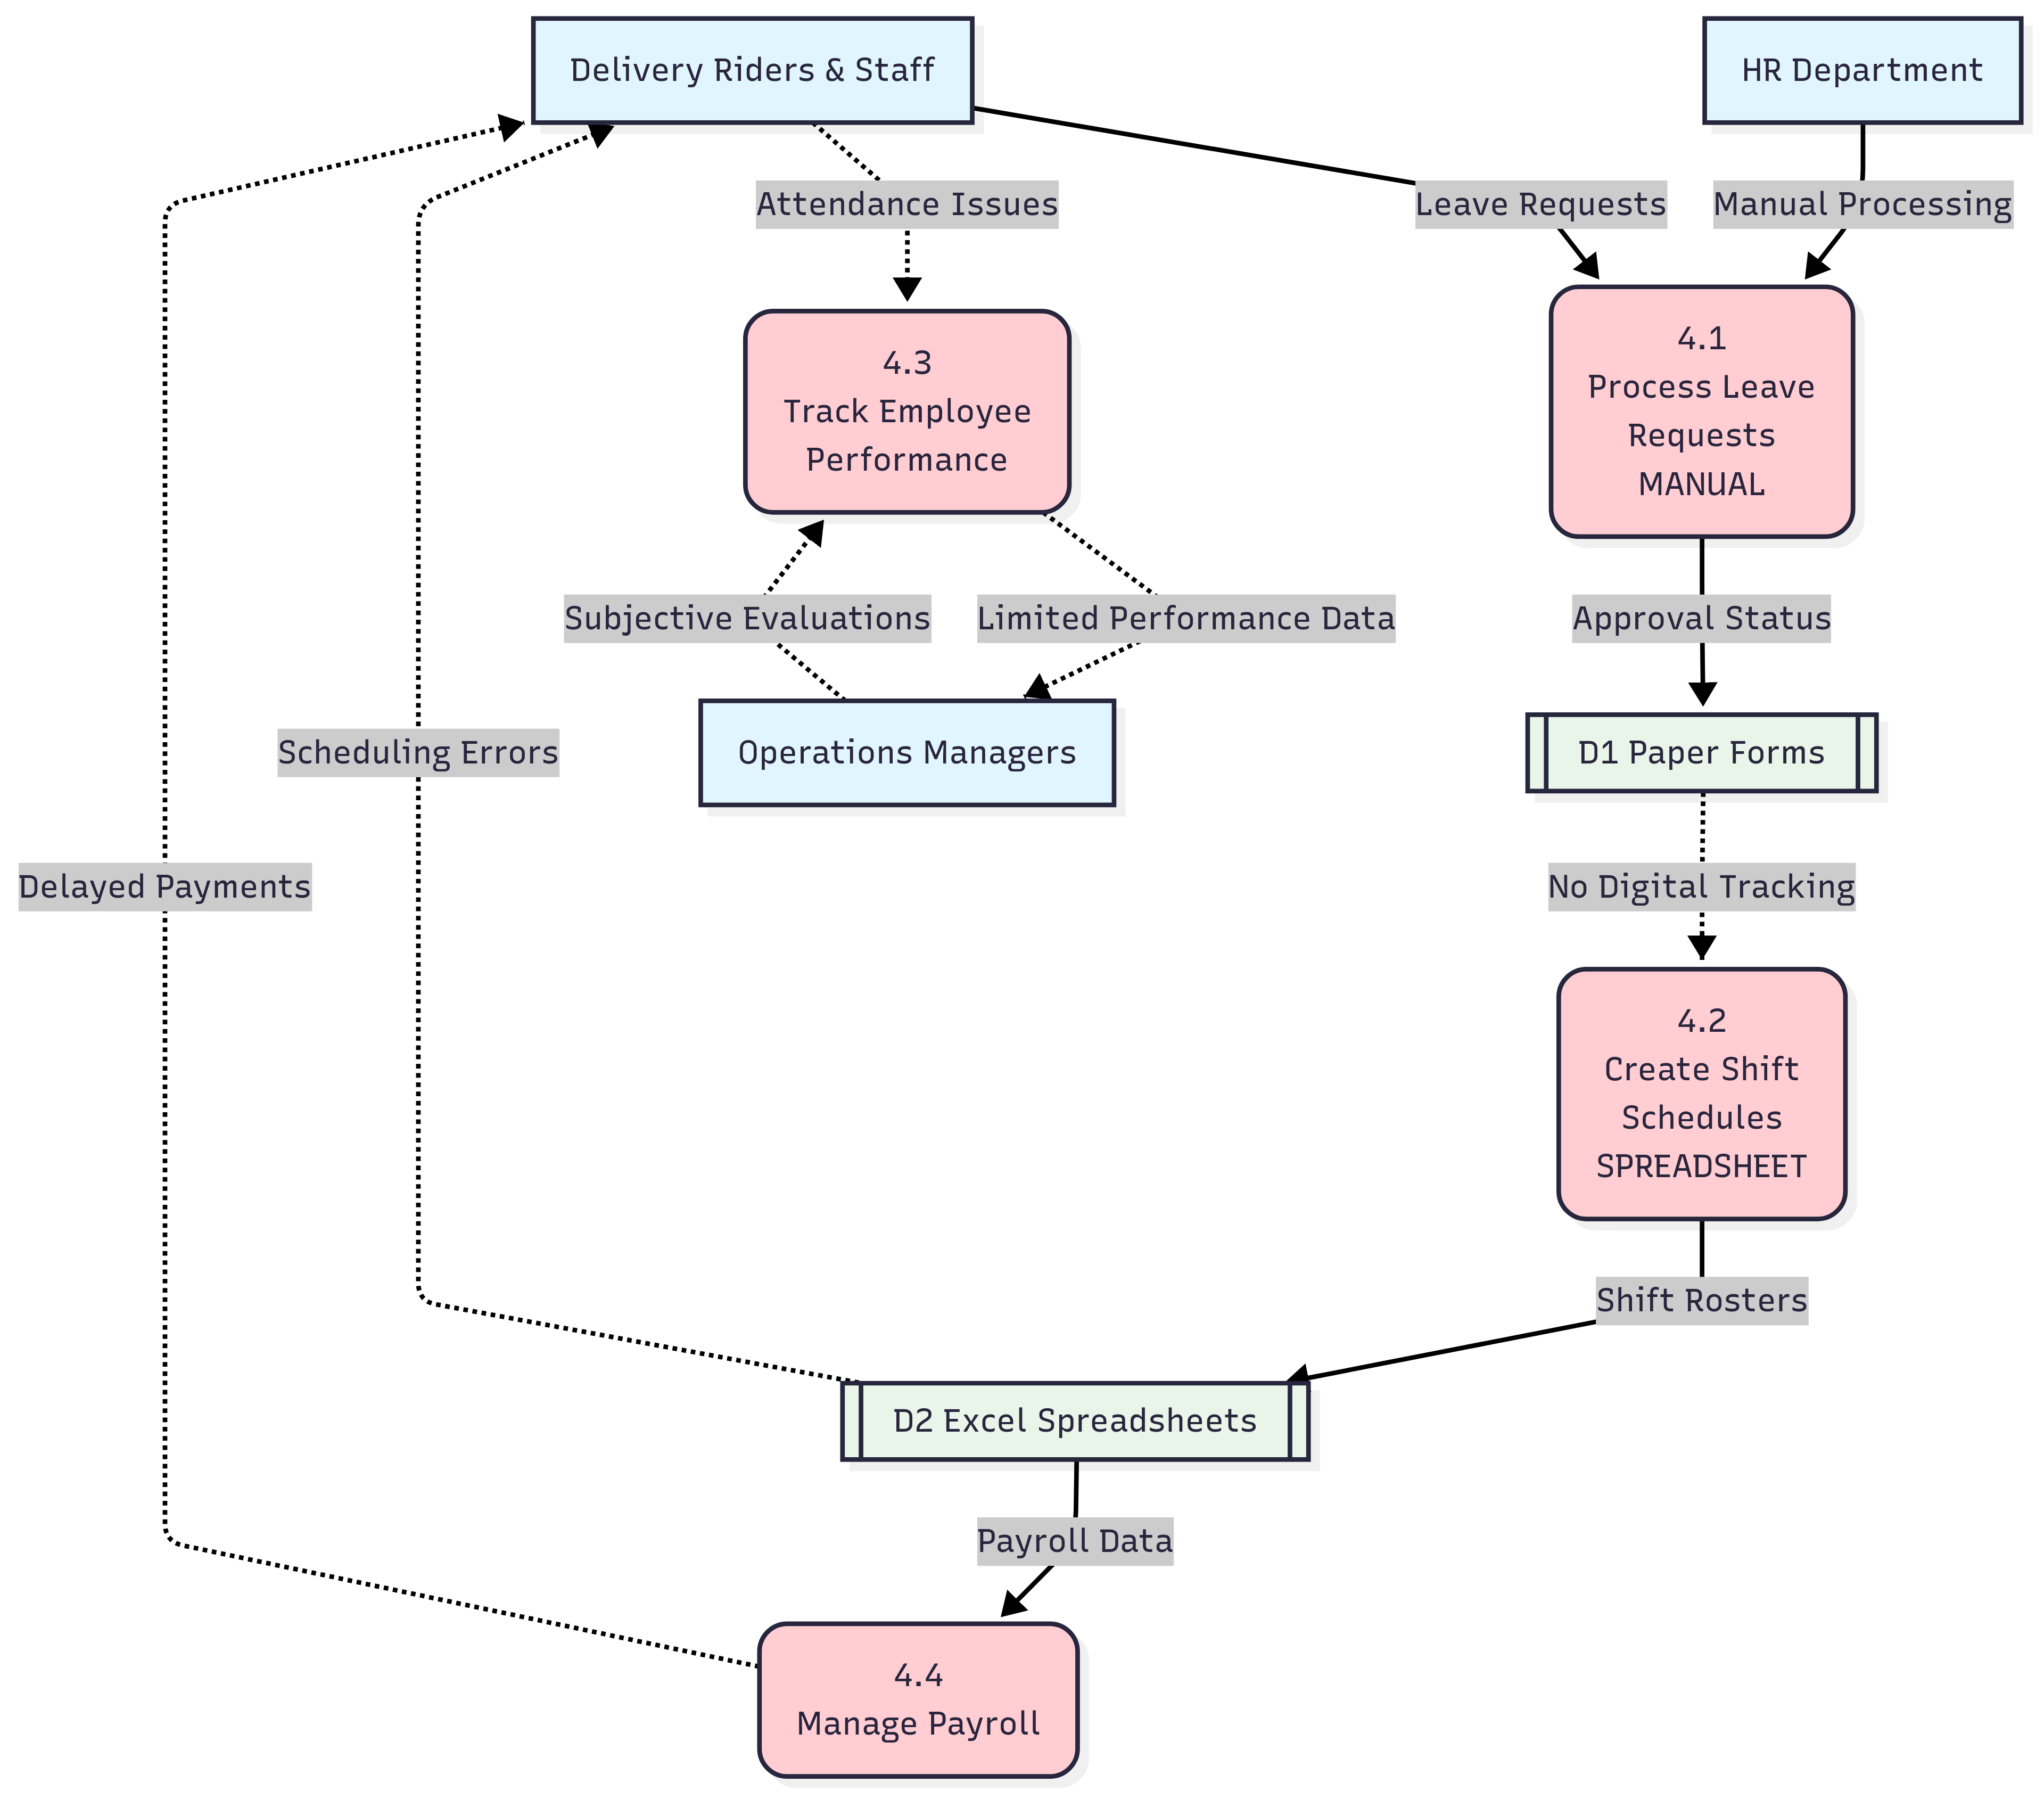
\includegraphics[width=1.0\textwidth]{p4_dfd_mermaid.png}
    \caption{DFD of HR and Workforce Management Subsystem}
    \label{fig:dfd_hr}
\end{figure}
\underline{\textit{DESCRIPTION:}} This DFD exposes the critical inefficiencies in Chaldal's human resource management system. Delivery Riders \& Staff submit leave requests to the 4.1 Process Leave Requests process, which is handled manually by the HR Department, creating bottlenecks and storing approvals in D1 Paper Forms with no digital tracking capability. The 4.2 Create Shift Schedules process relies on spreadsheet-based management, storing shift information in D2 Excel Spreadsheets, which frequently generates scheduling errors that impact Employees. The 4.3 Track Employee Performance process receives limited attendance data and relies on subjective evaluations from Operations Managers, lacking systematic performance recording. The 4.4 Manage Payroll process uses data from spreadsheets, often resulting in delayed payments to employees. Critically, the diagram shows two missing data stores: D3 Employee Database and D4 Performance Records (shown with dashed borders), highlighting the absence of integrated digital infrastructure. The numerous dashed data flows indicate problematic or inefficient processes, demonstrating how manual HR management creates operational bottlenecks, reduces transparency, and contributes to employee dissatisfaction and high turnover rates.

\paragraph{DFD for Problem 05: Under-Optimized Application and Over-Engineered IT Infrastructure}
\hfill \break
This DFD models the poor user experience resulting from the under-optimized mobile application, which is a symptom of misaligned engineering priorities.
\begin{figure}[H]
    \centering
    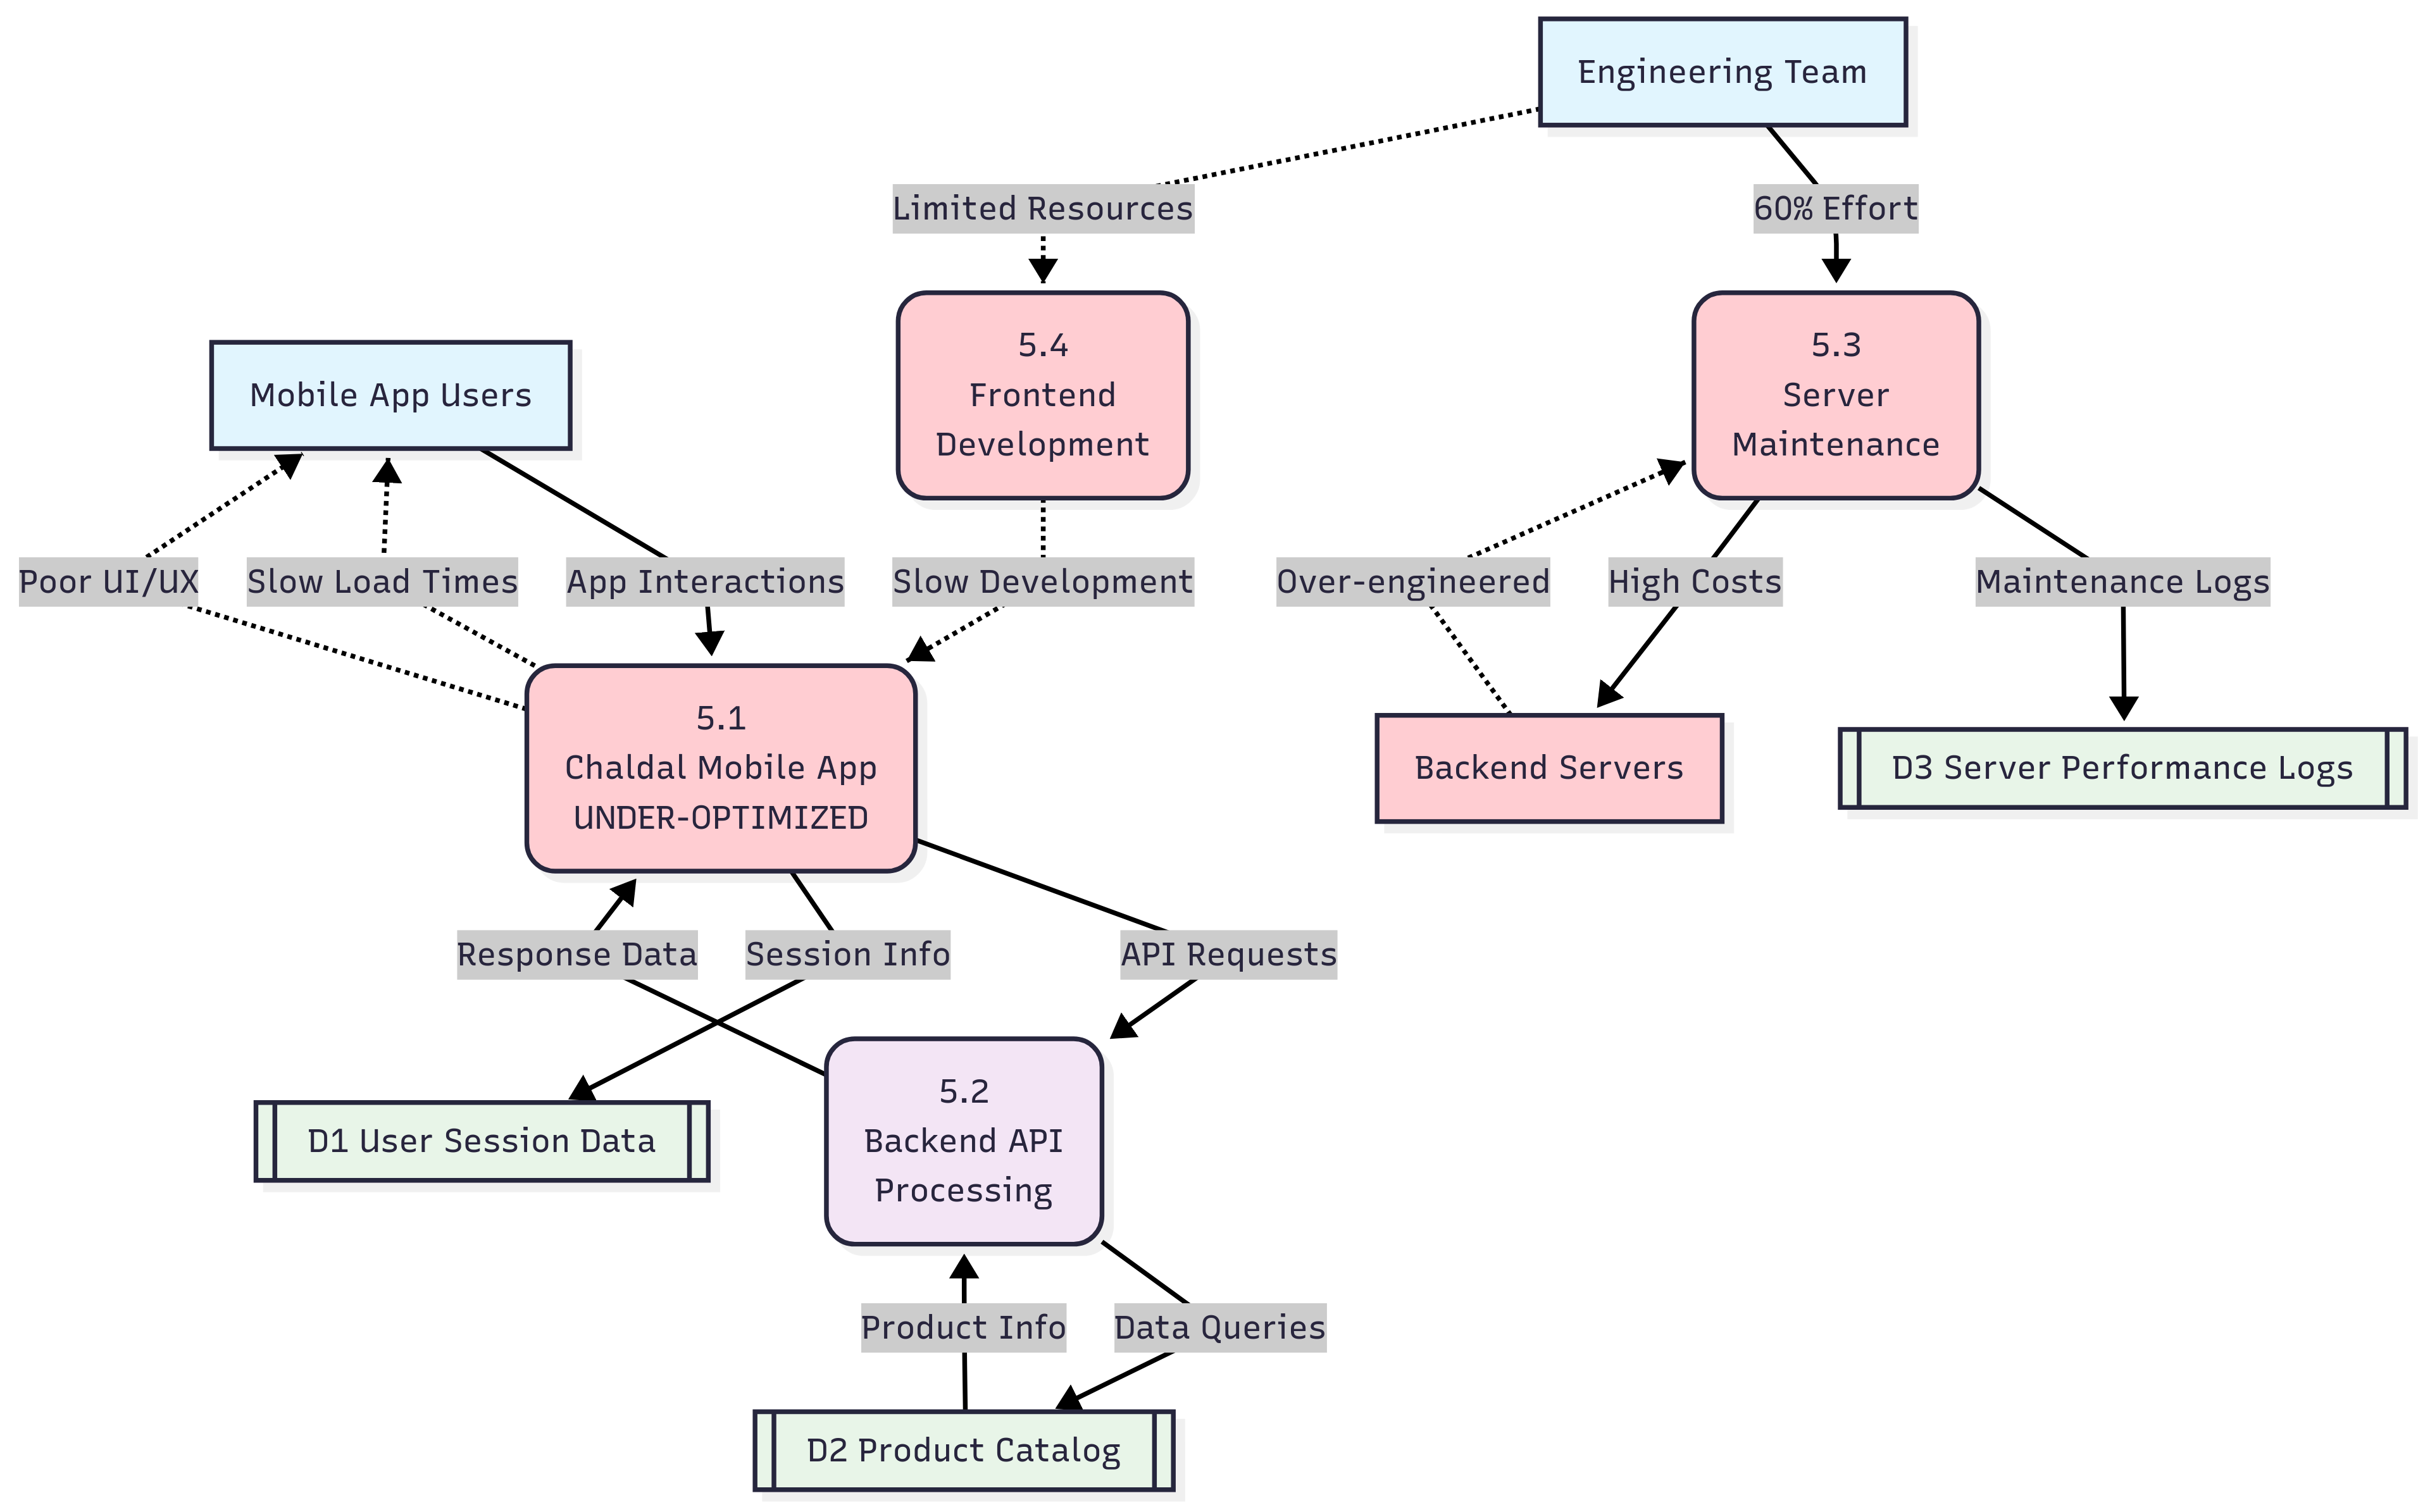
\includegraphics[width=1.0\textwidth]{p5_dfd_mermaid.png}
    \caption{DFD of IT Infrastructure and Mobile Application Subsystem}
    \label{fig:dfd_technical}
\end{figure}
\underline{\textit{DESCRIPTION:}} This DFD illustrates the misalignment between Chaldal's technical capabilities and user experience delivery. Mobile App Users interact with the 5.1 Chaldal Mobile App process, which is labeled "UNDER-OPTIMIZED" to highlight its performance issues. The app communicates with the 5.2 Backend API Processing process, which successfully retrieves product information from D2 Product Catalog, demonstrating that core functionality works. However, the app delivers slow load times and poor UI/UX back to users, creating customer dissatisfaction. The root cause is shown through resource allocation: the Engineering Team dedicates 60\% of their effort to the 5.3 Server Maintenance process for over-engineered Backend Servers, while providing limited resources to 5.4 Frontend Development. This creates a cycle where server maintenance generates high costs and maintenance logs in D3 Server Performance Logs, but the frontend development process receives insufficient attention, resulting in slow improvements to the user-facing application. The dashed lines indicate problematic data flows and resource constraints, demonstrating how over-investment in backend infrastructure at the expense of user experience optimization directly impacts customer retention and satisfaction in a competitive mobile-first market.

Each DFD provides a visual and descriptive analysis of the current system’s structure and pain points, supporting the identification of targeted improvements in subsequent chapters.

\subsection{Detailed Feasibility Analysis}
A feasibility study tests the viability of an idea, a project, or even a new business. The goal of a feasibility study is to emphasize potential problems that could occur if a project should be pursued.

The purpose of the feasibility study is to present the project parameters and potential solutions to the defined problem. Project constraints and limitations of expenditure are among the various factors that will determine viability. After brainstorming various potential solutions, we will elaborate on each of the solutions. We will obey three key considerations involved with feasibility analysis: Economic feasibility, Technical feasibility, and Behavioral feasibility.

As we have studied the present system of Chaldal, we have concluded three potential candidate systems, which are discussed in detail in the following sections.

\subsubsection{Root Cause Analysis of Identified Problems}
\begin{itemize} 
    \item \textbf{Problem 1: Lack of Profitability and Funding Constraints} Unsustainable Cost Structure Driven by a Misaligned IT Strategy. The foundational issue is that the company's largest operational expense—its over-engineered, on-premise IT infrastructure—is disproportionately high for its current revenue and order volume. This high, fixed cost creates negative unit economics, meaning the company may lose money on every order it processes. This financial drain prevents investment in growth, marketing, and competitive salaries, creating a negative feedback loop of poor performance that naturally deters new investors.
    \item \textbf{Problem 2: Product Sourcing and Supply Chain Inefficiencies} Reliance on a Reactive and Manual Procurement System. Chaldal lacks a centralized, data-driven platform for managing its vendors and supply chain. Procurement is handled through informal, manual coordination, making it impossible to enforce quality standards, track vendor performance objectively, or forecast demand accurately. This reactive approach, combined with an inadequate cold chain, leads directly to unreliable supply, price volatility, and significant product waste
    \item \textbf{Problem 3: Ineffective Customer Representative \& Delivery Operations} Underinvestment in the Workforce and Logistics Technology. This problem is a direct consequence of the financial instability detailed in Problem 1. The lack of funds prevents Chaldal from hiring, training, and retaining a professional, full-time delivery fleet. This forces a reliance on a less reliable part-time workforce and prevents investment in modern logistics software for automated dispatch and route optimization. The operational chaos is a symptom of a deeper financial inability to build a professional logistics arm.
    \item \textbf{Problem 4: Operational and HR Process Inefficiencies} Absence of a Digital HR Infrastructure. The core of this issue is the reliance on outdated, manual tools (paper forms, Excel spreadsheets) to manage a large and dynamic workforce. This manual approach is inherently unscalable, prone to human error, and creates significant administrative bottlenecks. It fosters an environment of perceived favoritism and inefficiency, which directly contributes to low employee morale and high turnover.
    \item \textbf{Problem 5: Under-Optimized Application and Over-Engineered IT Infrastructure} Misalignment of Engineering Resources. This is the technical manifestation of Problem 1. The engineering team's focus and budget are overwhelmingly dedicated to maintaining the complex, expensive, and oversized backend infrastructure. This leaves the frontend (the mobile app that customers actually use) critically under-resourced. The result is a poor core product, which harms customer retention and revenue, despite the powerful but inefficient engine running behind the scenes. The company is investing in the wrong part of its technology stack
\end{itemize}

\subsubsection{Candidate System 1: Integrated Supply Chain and Vendor Management System}
This system is designed to address the root causes of \textbf{Problem 2: Product Sourcing and Supply Chain Inefficiencies}. It focuses on creating a transparent, reliable, and efficient procurement ecosystem through technology.
\begin{itemize}
    \item \textbf{System Description:} This system involves developing a centralized digital platform that integrates vendor management, automated procurement, and real-time inventory tracking. Key features would include a vendor portal for suppliers to manage their product listings and view purchase orders, an automated reordering module based on predictive demand forecasting, and a quality control module to track vendor performance. It would also integrate cold chain logistics monitoring to ensure the freshness of perishable goods from the supplier to the micro-warehouse.
    \item \textbf{Technical Feasibility:} This system requires significant software development, particularly for the vendor portal and the predictive analytics engine. Integration with the existing inventory management system is crucial. The technology is mature and available. Chaldal's existing engineering team, with some specialized hiring in data science, can handle the development. The primary technical challenge would be the seamless integration with a diverse and often low-tech supplier base, requiring a simple, mobile-first vendor interface.
    \item \textbf{Behavioral Feasibility:} For Chaldal's procurement team, this system would represent a significant shift from manual, relationship-based sourcing to a data-driven process. Extensive training would be required. For vendors, adoption could be a hurdle, especially for smaller, less tech-savvy suppliers. A phased rollout, starting with larger vendors and providing clear incentives (e.g., faster payment processing), would be necessary to ensure buy-in and a smooth transition.
    \item \textbf{Economic Feasibility:} 
    \begin{itemize}
        \item \textbf{Initial Investment:} Approximately 80 Lakh BDT for software development, data integration, and initial vendor onboarding.
        \item \textbf{Annual Maintenance:}  Approximately 15 Lakh BDT.
        \item \textbf{Projected Savings:}  Expected to reduce product spoilage by 50\% and procurement costs by 10-15\% through direct sourcing, leading to annual savings of approximately 60-70 Lakh BDT.
        \item \textbf{Break-Even:}  Around 1.5 years.
        \item \textbf{Return on Investment (ROI):}  Estimated at 200\% within 3 years post-implementation.
    \end{itemize}
    \item \textbf{Challenges:} The main challenges include overcoming vendor resistance to technology, ensuring data accuracy in the predictive models, and the initial cost of development in a funding-constrained environment.
\end{itemize}

\subsubsection{Candidate System 2: Digital Workforce and Logistics Optimization Platform}
This system directly targets \textbf{Problem 3 (Ineffective Delivery Operations)} and \textbf{Problem 4 (HR Process Inefficiencies)} by automating workforce management and optimizing last-mile logistics.

\begin{itemize}
    \item \textbf{System Description:} This platform would be a comprehensive HR and logistics tool for managing Chaldal's frontline workforce (delivery riders and warehouse staff). It would feature modules for automated shift scheduling, digital leave requests, and attendance tracking. A key component would be a "smart" delivery assignment algorithm that allocates orders based on rider location, traffic conditions, and performance history. It would also include a digital payment reconciliation module to reduce the risks associated with Cash on Delivery (COD).
    \item \textbf{Technical Feasibility:} This requires developing a robust mobile-first application for employees and integrating it with the existing order management system. The logistics algorithm would need to integrate with a reliable mapping and traffic data provider (e.g., Google Maps API). The technology is readily available, and much of it can be built upon existing HR software frameworks, reducing development time. Chaldal's engineering team has the capability to build and integrate such a system.
    \item \textbf{Behavioral Feasibility:} This system would be highly beneficial for employees, offering transparency and fairness in scheduling and leave management. Delivery riders would benefit from optimized routes and clearer performance metrics. Management would need to adapt to a more data-driven approach to workforce management. The primary behavioral challenge would be ensuring consistent use of the app by all staff and training them effectively on the new digital processes.
    \item \textbf{Economic Feasibility:} 
    \begin{itemize}
        \item \textbf{Initial Investment:} Approximately 60 Lakh BDT for software development and integration.
        \item \textbf{Annual Maintenance:}  Approximately 10 Lakh BDT.
        \item \textbf{Projected Savings:}  Expected to improve delivery efficiency by 20\% (reducing fuel costs and time per delivery) and reduce administrative HR time by 75\%. This would translate to annual savings of around 50 Lakh BDT.
        \item \textbf{Break-Even:}  Approximately 1.5 - 2 years.
        \item \textbf{Return on Investment (ROI):} Estimated at 150\% within 3 years post-implementation.
    \end{itemize}
    \item \textbf{Challenges:} The primary challenges are the cost of API licensing for mapping services, ensuring the algorithm is accurately calibrated for Dhaka's unique traffic patterns, and managing the change process with the workforce.
\end{itemize}
\subsubsection{Candidate System 3: Lean IT Infrastructure and Frontend App Optimization}

This system is a direct response to \textbf{Problem 1 (Lack of Profitability)} and \textbf{Problem 5 (Under-Optimized App and Over-Engineered IT)}. It focuses on reducing operational costs and improving the core customer-facing product.

\begin{itemize}
    \item \textbf{System Description:} This is a two-part strategic initiative. First, it involves a systematic migration of Chaldal's over-engineered proprietary backend from on-premise servers to a lean, scalable cloud-based infrastructure (e.g., AWS or Google Cloud). This would involve refactoring parts of the system to use managed services, reducing the need for constant manual maintenance. Second, it involves a dedicated project to re-architect and optimize the customer-facing mobile application, focusing on improving performance, user experience (UX), and implementing modern, responsive animations.
    \item \textbf{Technical Feasibility:} This is a highly technical project that would require careful planning and execution to avoid service disruptions. A phased migration to the cloud is feasible. The app optimization would require a dedicated frontend development team with expertise in modern mobile frameworks. While technically complex, it is a standard process for maturing tech companies. Chaldal's engineering team would need to be restructured to create this focus.
    \item \textbf{Behavioral Feasibility:} This would require a significant cultural shift within the engineering team, moving from a focus on building proprietary infrastructure to leveraging managed services and prioritizing the user experience. It could face resistance from engineers invested in the current system. For customers, the change would be overwhelmingly positive, leading to a faster, more reliable, and more enjoyable user experience, likely increasing engagement and retention.
    \item \textbf{Economic Feasibility:} 
    \begin{itemize}
        \item \textbf{Initial Investment:} Approximately 1 Crore BDT for cloud migration consultancy, initial cloud setup costs, and hiring specialized frontend developers.
        \item \textbf{Annual Maintenance:}  Projected to reduce IT infrastructure and maintenance costs by 40-50\% annually, saving upwards of 1 Crore BDT per year. Improved app performance is estimated to increase customer retention by 10\%, adding significant long-term value.
        \item \textbf{Projected Savings:} Approximately 1 Crore BDT annually from reduced infrastructure costs and increased customer lifetime value.Android app optimization is expected to reduce churn by 15\%, leading to higher revenue retention.
        \item \textbf{Total Cost of Ownership (TCO):} The shift to a cloud-based infrastructure is expected to lower the total cost of ownership by reducing hardware and maintenance costs while improving scalability and performance.
        \item \textbf{Break-Even:} Less than 1.5 years.
        \item \textbf{Return on Investment (ROI):} Estimated at 180\% within 3 years post-implementation.
    \end{itemize}
    \item \textbf{Challenges:} The main challenges include managing the technical complexity of the migration without disrupting service, overcoming internal resistance to change, and ensuring that the app optimization meets user expectations in a competitive market. Other challenges include the risk of downtime during migration, the potential for internal resistance to changing the tech stack, and the upfront cost of the project.
\end{itemize}

\subsection{Comparative Analysis of Candidate Systems}
To provide a clear, data-driven basis for selecting the most appropriate solution for Chaldal, this section presents a comparative analysis of the three proposed candidate systems. The comparison is structured using a series of matrices that evaluate each system based on key financial metrics, performance attributes, and cost factors. This structured approach allows for a direct comparison of the systems' respective strengths and weaknesses, leading to a well-reasoned recommendation. The values used in these tables are derived from the economic feasibility sections and are intended to provide a relative measure of each system's viability and potential impact.


\begin{table}[h]
\centering
\caption{Comparison of Proposed Systems for Chaldal}
\begin{tabular}{|p{3cm}|p{4cm}|p{4cm}|p{4cm}|}
\hline
\textbf{Criteria} & System 1: Integrated Supply Chain \& Vendor Management & System 2: Digital Workforce \& Logistics Optimization & System 3: Lean IT \& Frontend App Optimization \\ \hline

Initial Cost (BDT) & 80,00,000 & 60,00,000 & 1,00,00,000 \\ \hline

Annual Maintenance (BDT) & 15,00,000 & 10,00,000 & Varies (Cloud Costs) \\ \hline

Training Costs (BDT) & High (Vendor \& Staff) & Moderate (Staff) & Moderate (Engineers) \\ \hline

Projected Annual Savings (BDT) & 65,00,000 & 50,00,000 & 1,00,00,000+ \\ \hline

Break-Even Period & $\sim$1.5 years & $\sim$1.5--2 years & $\sim$1.5 years \\ \hline

Operational Impact & Improved product quality, reduced stockouts & Increased delivery speed, higher staff efficiency & Reduced IT costs, improved user experience \\ \hline

Risks & Vendor adoption, data accuracy & API costs, change management & Migration downtime, internal resistance \\ \hline
\end{tabular}
\end{table}

The comparative analysis reveals that while System 3 has the highest initial investment, it offers the greatest potential for long-term cost savings and operational efficiency improvements. System 2 provides a balanced approach with moderate costs and significant operational benefits, making it an attractive option for immediate implementation.

\begin{table}[h]
\centering
\caption{Performance Evaluation Matrix}
\begin{tabular}{|p{3cm}|p{1.5cm}|p{1.5cm}|p{1.5cm}|p{1.5cm}|p{1.5cm}|p{1.5cm}|p{1.5cm}|}
\hline
Evaluation Criteria & Weighting Factor & Candidate 1 Rating & Candidate 1 Score & Candidate 2 Rating & Candidate 2 Score & Candidate 3 Rating & Candidate 3 Score \\ \hline

User-Friendly & 5 & 3 & 15 & 4 & 20 & 5 & 25 \\ \hline

Employee-Friendly & 4 & 3 & 12 & 5 & 20 & 3 & 12 \\ \hline

Use of Technology & 4 & 4 & 16 & 4 & 16 & 5 & 20 \\ \hline

Reliability & 4 & 4 & 16 & 3 & 12 & 5 & 20 \\ \hline
\end{tabular}
\end{table}

This performance evaluation matrix compares the three candidate systems across four critical performance dimensions, each weighted according to its importance to Chaldal's business objectives. The ratings are scored on a scale of 1-5, with higher scores indicating better performance. System 3 demonstrates superior user-friendliness and technology utilization, making it the strongest candidate for addressing customer experience challenges, while System 2 excels in employee-friendliness, reflecting its focus on workforce optimization.



\begin{table}[h]
\centering
\caption{Cost Evaluation Matrix}
\begin{tabular}{|p{4.5cm}|p{1.2cm}|p{1.2cm}|p{1.2cm}|p{1.2cm}|p{1.2cm}|p{1.2cm}|p{1.2cm}|}
\hline
Evaluation Criteria & Weight Factor & C1 Rating & C1 Score & C2 Rating & C2 Score & C3 Rating & C3 Score \\ \hline

System Development & 4 & 3 & 12 & 4 & 16 & 3 & 12 \\ \hline

System Operation & 5 & 4 & 20 & 4 & 20 & 5 & 25 \\ \hline

Technical Support & 4 & 3 & 12 & 3 & 12 & 4 & 16 \\ \hline
\end{tabular}
\end{table}

This cost evaluation matrix assesses the three candidate systems across key cost dimensions using weighted scoring methodology. System 3 achieves the highest overall score due to its superior operational efficiency and long-term cost benefits. While Systems 1 and 2 require moderate development investments, System 3's cloud-based architecture offers the most favorable total cost of ownership despite higher initial development costs.


\begin{table}[h]
\centering
\caption{Qualitative Evaluation Matrix}
\begin{tabular}{|p{4.5cm}|p{3cm}|p{3cm}|p{3cm}|}
\hline
\textbf{Evaluation Criteria} & \textbf{Candidate System-1} & \textbf{Candidate System-2} & \textbf{Candidate System-3} \\ \hline

\multicolumn{4}{|l|}{\textbf{Performance}} \\ \hline

User-friendly & 75\% & 85\% & 98\% \\ \hline

Employee-friendly & 70\% & 95\% & 70\% \\ \hline

Use of Technology & 85\% & 80\% & 95\% \\ \hline

Reliability & 80\% & 75\% & 95\% \\ \hline

\multicolumn{4}{|l|}{\textbf{Cost}} \\ \hline

System Development & High & Medium & High \\ \hline

System Operation & Medium & Medium & Low \\ \hline

Technical Support & Medium & Medium & Medium \\ \hline
\end{tabular}
\end{table}

This qualitative evaluation matrix provides a comprehensive comparison of the three candidate systems across key performance and cost dimensions. The percentages for performance criteria reflect each system's effectiveness in meeting user expectations, employee satisfaction, technological advancement, and operational reliability. System 3 demonstrates superior performance across most criteria, particularly in user-friendliness (98\%) and technology utilization (95\%), while System 2 excels in employee-friendliness (95\%), making it ideal for workforce optimization initiatives.

\subsection{Selecting the best candidate system}
Based on the detailed feasibility and comparative analysis, \textbf{System 3: Lean IT \& Frontend App Optimization} is the most critical and feasible option for Chaldal to pursue immediately. This recommendation is based on its potential for high impact and its strategic importance in addressing foundational issues.

The primary reasons for this selection are its direct impact on profitability and the core customer experience. The system's focus on migrating to a lean cloud infrastructure directly tackles the massive operational cost of the over-engineered IT system, which is a primary driver of the company's unprofitability. The projected annual savings of over 1 Crore BDT and a rapid break-even period of under 1.5 years make this a compelling financial decision. Simultaneously, optimizing the under-performing mobile application addresses the most significant customer-facing issue. Since the majority of users interact with Chaldal via the mobile app, improving its performance and user experience is crucial for customer retention and satisfaction, making the service more competitive against rivals.

Furthermore, this system addresses two of the most deeply interconnected problems—financial instability and poor customer retention—creating a more stable foundation for the business. By reducing IT costs, capital is freed up for investment in other critical areas. By improving the app, Chaldal strengthens its primary channel for revenue generation. While the initial investment is the highest among the options, the long-term ROI is also the greatest, not just in terms of direct cost savings, but in building a scalable, reliable, and modern technology platform.

However, in the medium to long term, a phased implementation of the other systems would be highly beneficial. Once financial stability is improved and the core technology platform is modernized through System 3, Chaldal will be in a much stronger position to implement \textbf{System 2: Digital Workforce \& Logistics Optimization} to enhance operational efficiency and employee satisfaction, followed by \textbf{System 1: Integrated Supply Chain} to improve product quality and vendor relationships. This strategic sequencing ensures that foundational problems are solved first, creating the stability needed for subsequent operational enhancements.

\subsection{Cost-Benefit Analysis}
We know, cost-benefit analysis is a process by which organizations can estimate the cost and benefits of decisions, systems, or projects to find the most effective alternatives. By providing a clear view of the results of an action, cost-benefit analysis is an extremely useful tool in developing business strategy, evaluating new projects, or making resource allocation decisions. So, we developed a cost and benefit analysis model in this report for the recommended candidate system. Our model is developed by defining the benefits of a decision as well as the associated costs and subtracting the costs from the benefits.

\subsubsection{Cost Breakdown:}
A breakdown of the costs involving the recommended candidate system (System 3) has been shown below. Our goal is to optimize Chaldal's IT infrastructure and mobile application to reduce operational costs, enhance the user experience, and improve customer retention. The total costs primarily involve a one-time investment in cloud migration consultancy and frontend development, alongside ongoing annual costs for cloud services and maintenance. The most significant initial cost is for the strategic project to modernize the tech stack.


\begin{table}[h]
\centering
\caption{Cost Breakdown for Candidate System 3}
\begin{tabular}{|p{9cm}|p{3cm}|}
\hline
\textbf{Costs} & \textbf{Amount (BDT)} \\ \hline

Cloud Migration \& Consultancy (Initial) & 40,00,000 \\ \hline

Frontend App Development (Initial) & 50,00,000 \\ \hline

Staff Training (Initial) & 10,00,000 \\ \hline

Cloud Services (Annual) & 35,00,000 \\ \hline

Licensing and Maintenance (Annual) & 10,00,000 \\ \hline

\multicolumn{2}{|l|}{\textbf{Total Initial Costs:}} \\ \hline
\multicolumn{2}{|r|}{1,00,00,000} \\ \hline

\multicolumn{2}{|l|}{\textbf{Ongoing Annual Costs:}} \\ \hline
\multicolumn{2}{|r|}{45,00,000} \\ \hline
\end{tabular}
\end{table}

\subsubsection{Benefit Breakdown:}
A breakdown of the anticipated benefits of implementing Candidate System 3 is shown below. As per our calculations, the main benefits include significant annual cost savings from reduced IT infrastructure overhead and a substantial increase in revenue driven by improved customer retention due to a better app experience. The total annual benefits are projected to be 1,40,00,000 BDT, which fairly surpasses the ongoing annual costs.

\begin{table}[h]
    \centering
    \caption{Benefit Breakdown for Candidate System 3}
    \begin{tabular}{|p{10cm}|p{3cm}|}
        \hline
        \textbf{Benefits} & \textbf{Amount (BDT)} \\ \hline
        Reduced IT Infrastructure \& Maintenance Cost (Annual) & 1,00,00,000 \\ \hline
        Increased Revenue from Improved Retention Rate (Annual) & 40,00,000 \\ \hline
        \multicolumn{2}{|l|}{\textbf{Total Annual Benefits:}} \\ \hline
        \multicolumn{2}{|r|}{1,40,00,000} \\ \hline
    \end{tabular}
\end{table}

\subsubsection{Break-Even Analysis:}
A Break-Even Analysis helps determine when the benefits of an investment will cover its costs. For the IT optimization and app improvement project, we want to calculate the break-even point, where the total cumulative benefits equal the total cumulative costs. The summary of our cost-benefit analysis is shown below:
\begin{itemize}
    \item \textbf{Initial Costs:} This is the up-front investment needed to implement the system. In this case, it's 1,00,00,000 BDT.
    
    \item \textbf{Ongoing Costs:} These are the yearly costs required to maintain the system (e.g., cloud services, licensing), which total 45,00,000 BDT annually.
    
    \item \textbf{Annual Benefits:} The system is expected to generate 1,40,00,000 BDT in annual benefits (cost savings and new revenue).
    
    \item \textbf{Net Annual Benefit:} Each year, the system generates 95,00,000 BDT in net annual benefits (total annual benefits minus ongoing costs).
\end{itemize}
The break-even analysis table showing the cumulative costs and benefits over time, along with the net benefits each year, is given below:

\begin{table}[h]
    \centering
    \caption{Cumulative Costs and Benefits Analysis}
    \resizebox{\textwidth}{!}{%
    \begin{tabular}{|l|r|r|r|}
        \hline
        \textbf{Year} & \textbf{Cumulative Costs (BDT)} & \textbf{Cumulative Benefits (BDT)} & \textbf{Net Benefits (BDT)} \\ \hline
        0 (Initial) & 1,00,00,000 & 0 & -1,00,00,000 \\ \hline
        1 & 1,45,00,000 & 1,40,00,000 & -5,00,000 \\ \hline
        2 & 1,90,00,000 & 2,80,00,000 & +90,00,000 \\ \hline
        3 & 2,35,00,000 & 4,20,00,000 & +1,85,00,000 \\ \hline
    \end{tabular}%
    }
\end{table}

To calculate the break-even point in years, we use the formula where we divide initial costs (1,00,00,000 BDT) by net annual benefits (95,00,000 BDT). The result nearly sums up to 1.05 years. The break-even analysis graph is shown below:

\begin{figure}[H]
    \centering
    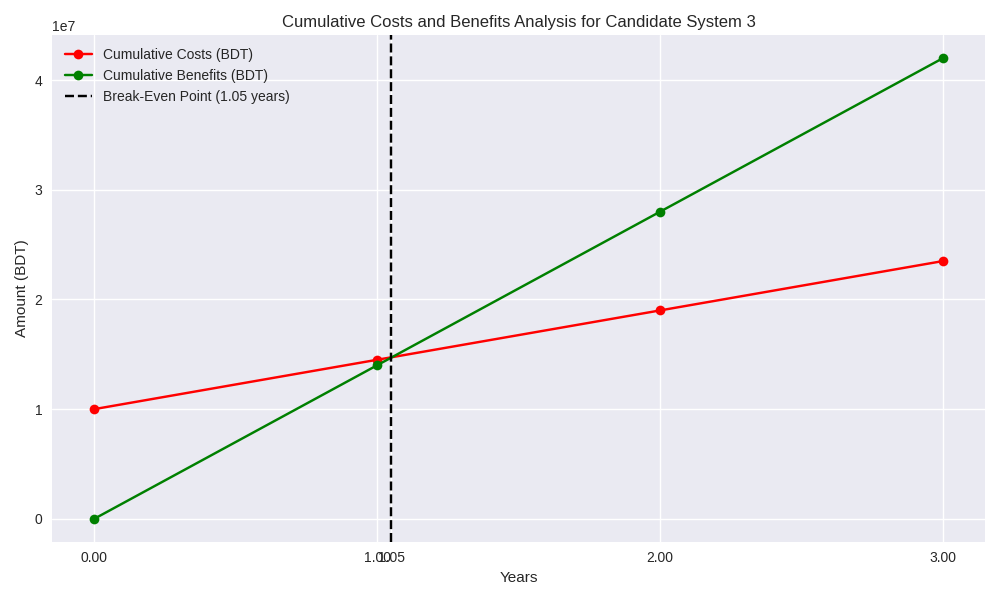
\includegraphics[width=1.0\textwidth]{break-even.png}
    \caption{Break-Even Analysis Graph for Candidate System 3}
    \label{fig:break-even-analysis}
\end{figure}

\subsection{Conclusion}
In conclusion, this analysis phase has transformed the initial problem recognition into a data-driven understanding of Chaldal's challenges, providing clear pathways for resolution. The interconnected nature of the problems necessitates a strategic approach that prioritizes foundational improvements in technology and financial stability before addressing operational refinements. The recommended Candidate System 3, with its break-even point of 1.05 years and substantial long-term returns, offers a critical intervention for financial sustainability and customer retention. With proper implementation, Chaldal can transition from its current operational struggles to a position of technological efficiency, financial stability, and competitive advantage in Bangladesh's evolving e-commerce landscape.

\newpage
% --- MAIN CONTENT ---
{\Large\bfseries\color{RoyalBlue}Chapter 4}
\vspace{0.8em}
\section{Design}
\vspace{0.6em}
\subsection{Introduction}
Systems design is the procedure of defining functions of a system like modules, architecture, diagram and their interfaces and data for a system based on the specialised requirements. It is the process of defining, developing and designing systems which ensures the specific needs and requirements of a business and organisation. Vital activities in system design and development include developing. System-level technical requirements and top-level system designs and assessing the design's ability to meet the system requirements.

A systemic approach is required for a coherent and well-running system. Bottom-Up or Top-Down approach is required to take into account all related variables of the system. A designer uses the modelling languages to express the information and knowledge in a structure of a system that is defined by a consistent set of rules and definitions. The designs can be defined in graphical or textual modelling languages. System-level technical requirements describe the users' needs and provide information for the finished system to meet legal restrictions, adhere to regulations, and inter-operate or integrate effectively with other systems. We can say that system design ranges from discussing the system requirements to product development. System development creates or alters the system so that the processes, practices and methodologies are changed to develop the system.

\subsection{DFD of the Proposed System}

\subsubsection{Overview and Purpose}
Start with a brief introduction to the diagram.

\begin{itemize}[leftmargin=*]
    \item \textbf{What it is:} This Level 0 Data Flow Diagram (DFD) provides a high-level, "bird's-eye view" of the entire proposed Chaldal e-commerce and logistics ecosystem.
    \item \textbf{Its Purpose:} It illustrates the primary functions (processes), key information repositories (data stores), and the external entities the system interacts with. Crucially, it visualizes the new, integrated architecture after the implementation of the recommended System 3: Lean IT \& Frontend App Optimization.
    \item \textbf{The Core Idea:} The diagram shows a shift from a simple transactional system to a lean, intelligent, and financially sustainable platform.
\end{itemize}

\begin{figure}[H]
    \centering
    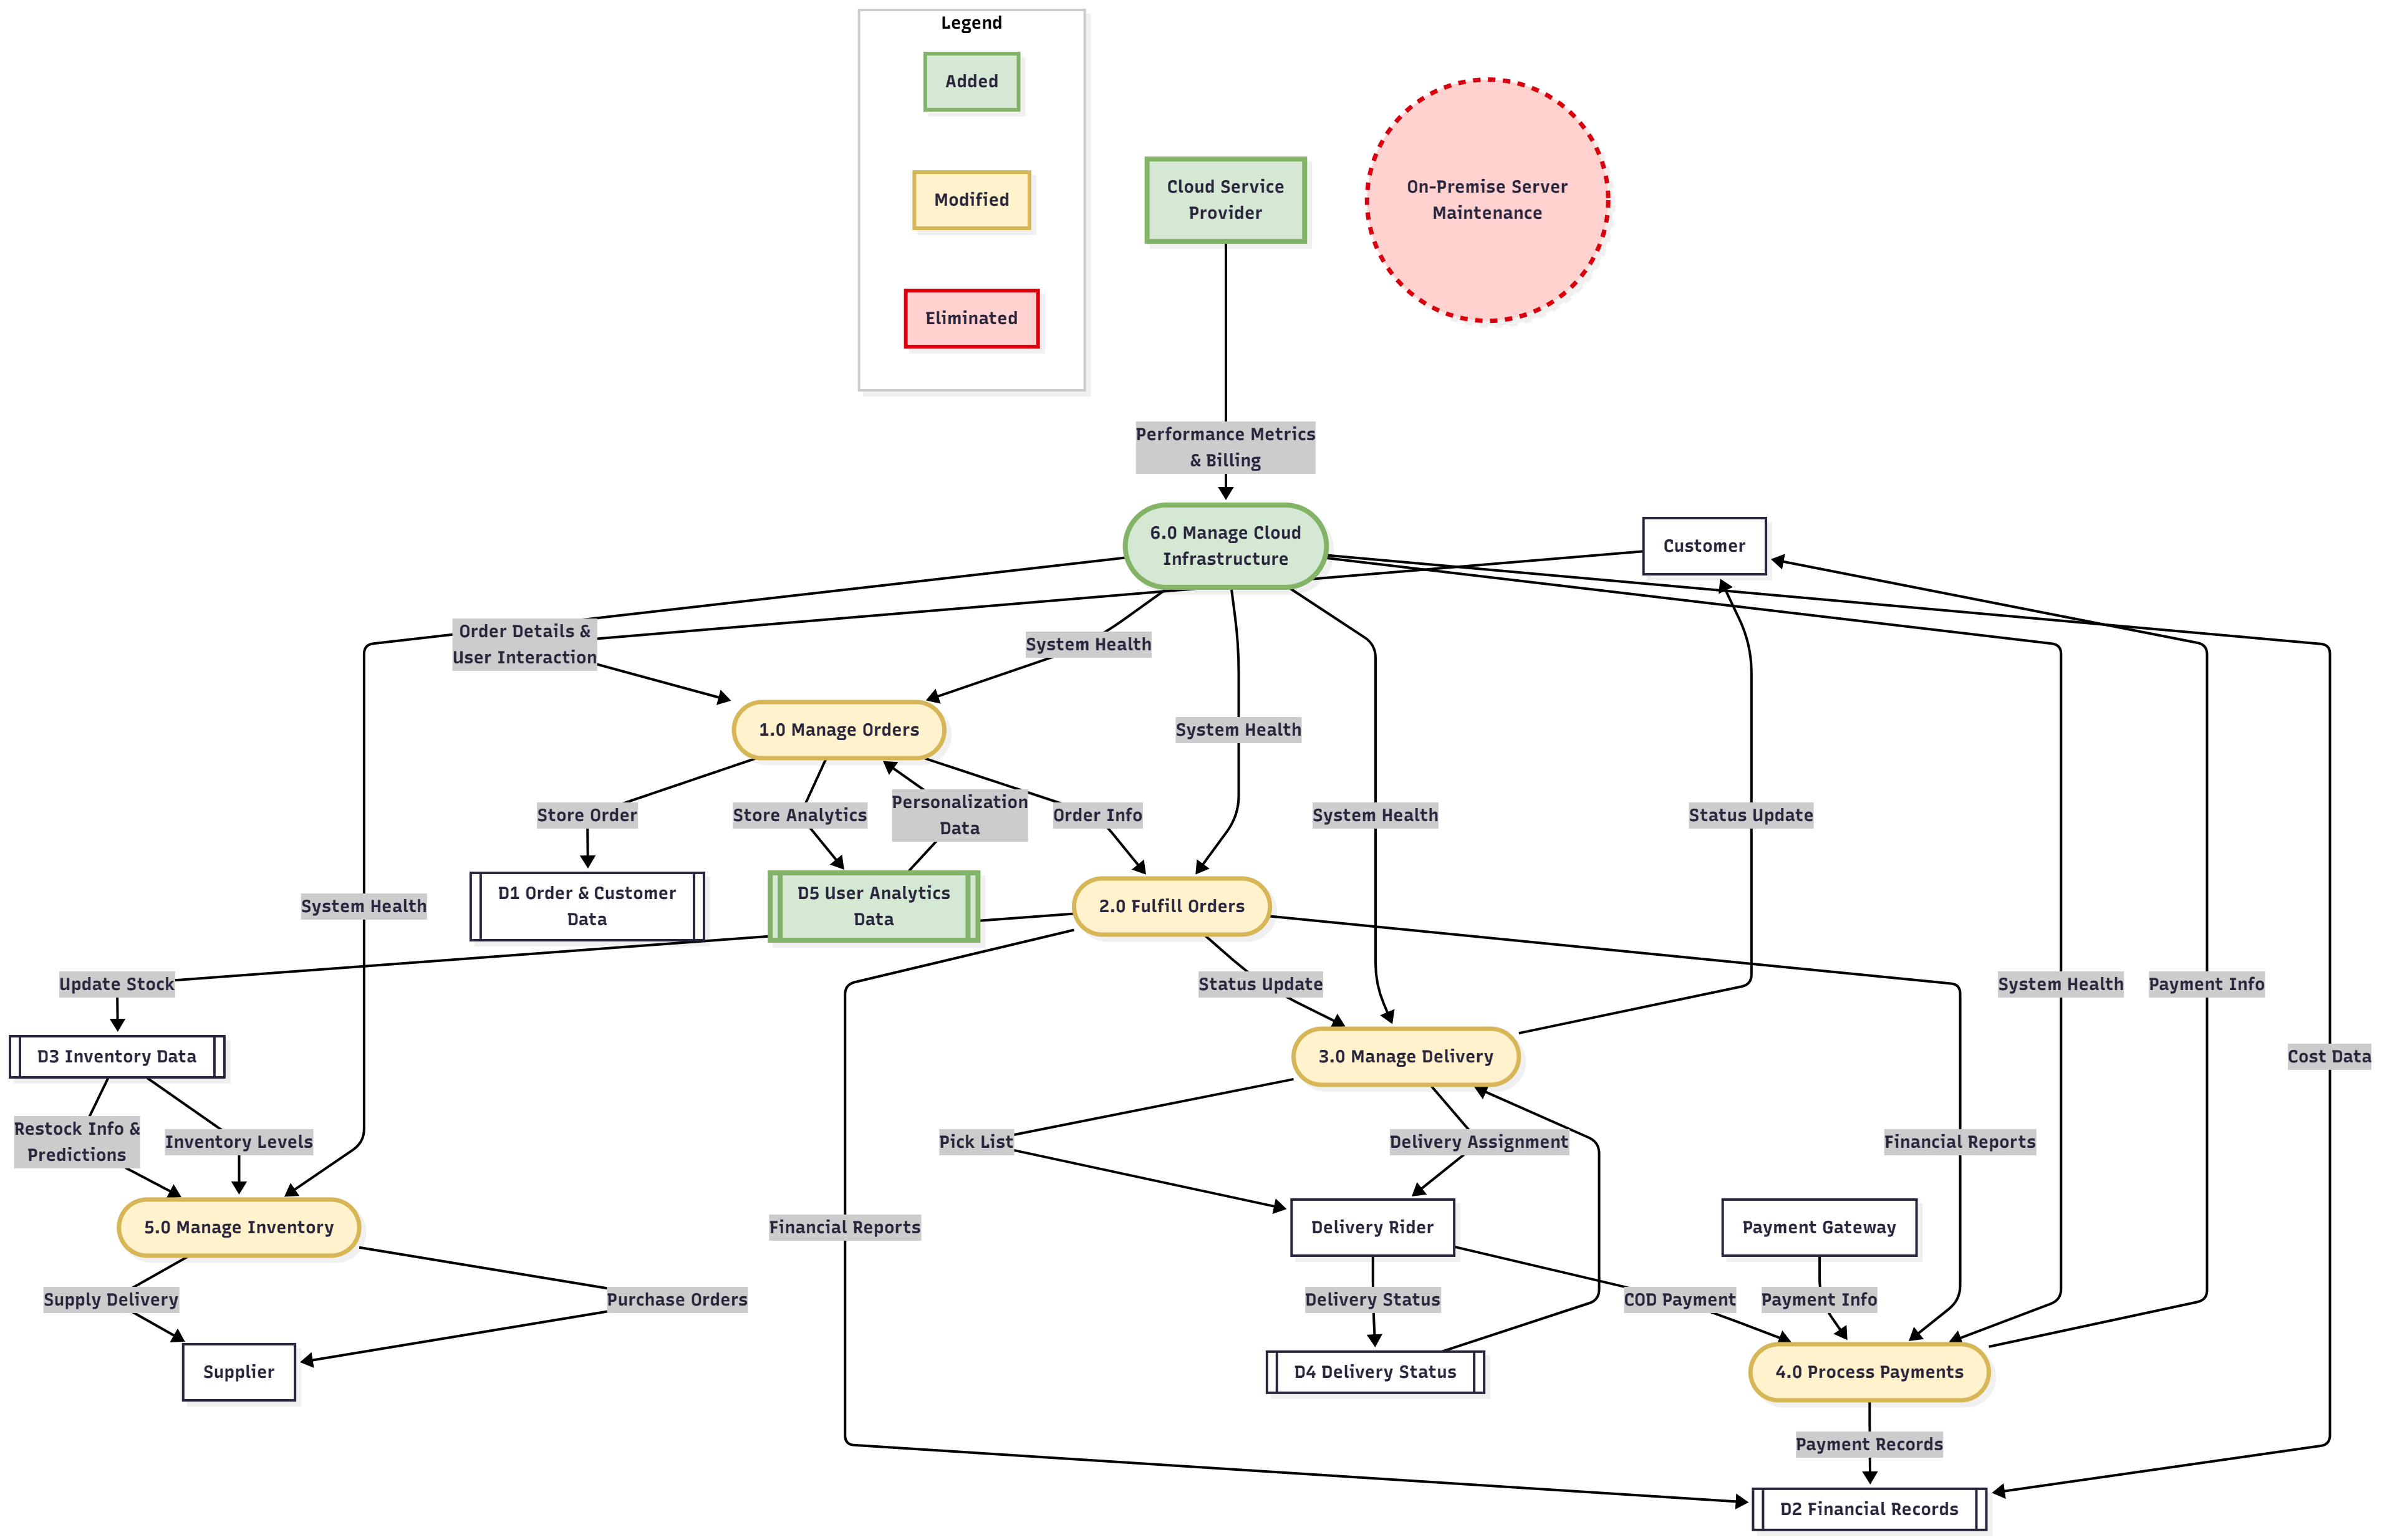
\includegraphics[width=1\textwidth]{new_dfd/level0_3.png}
    \caption{Proposed Level 0 DFD}
    \label{fig:Proposed Level 0 DFD}
\end{figure}



\subsubsection{Component Description}
Next, systematically describe each component shown in the diagram. This gives clarity to each element's role.

\textbf{External Entities (Actors)}

These are the people or systems that interact with the Chaldal system from the outside.

\begin{itemize}
    \item \textbf{Customer:} The primary user who initiates the process by browsing, placing orders, and making payments. In the new system, they also provide valuable User Interaction data.
    \item \textbf{Supplier:} The entity that provides the products (groceries, etc.) to be stocked in the inventory.
    \item \textbf{Payment Gateway:} A third-party service (like bKash, Nagad, or a bank) that processes digital financial transactions.
    \item \textbf{Delivery Rider:} The frontline employee responsible for the physical last-mile delivery of orders to the customer.
    \item \textbf{Cloud Service Provider (Added):} A new and critical external entity (e.g., Amazon Web Services, Google Cloud). It provides the scalable, on-demand infrastructure that the entire system runs on, replacing the old, costly physical servers.
\end{itemize}

\textbf{Processes (The System's Functions)}

These are the core activities the system performs to transform data.

\begin{itemize}
    \item \textbf{1.0 Manage Orders (Modified):} This process now does more than just record orders. Fueled by data from the new analytics store, it also handles personalization to improve the customer experience.
    \item \textbf{2.0 Fulfill Orders (Modified):} Handles the internal logistics of picking and packing items from the micro-warehouses. It's now more reliable due to the stable cloud backend.
    \item \textbf{3.0 Manage Delivery (Modified):} Coordinates the dispatch of delivery riders and tracks the order status until it reaches the customer.
    \item \textbf{4.0 Process Payments (Modified):} Manages all financial transactions, including digital payments and Cash on Delivery (COD).
    \item \textbf{5.0 Manage Inventory (Modified):} Manages stock levels and automates the reordering process from suppliers.
    \item \textbf{6.0 Manage Cloud Infrastructure (Added):} A new, vital process that monitors the performance and, most importantly, the cost of the cloud services, ensuring the IT infrastructure remains lean and budget-friendly.
\end{itemize}

\textbf{Data Stores (Information Repositories)}

These are where the system stores its essential information.

\begin{itemize}
    \item \textbf{D1 Order \& Customer Data:} Stores all information related to customer accounts and their specific orders.
    \item \textbf{D2 Financial Records:} The central repository for all financial data, including sales, costs, and payment records.
    \item \textbf{D3 Inventory Data:} Keeps a real-time record of all product stock levels across the micro-warehouses.
    \item \textbf{D4 Delivery Status:} A real-time log of the status of all ongoing deliveries.
    \item \textbf{D5 User Analytics Data (Added):} A new and strategic data store that captures how users interact with the optimized mobile app (e.g., what they search for, how long they view items). This data is the fuel for personalization and business intelligence.
\end{itemize}

\subsubsection{Information Flow and System Walkthrough}
Describe how data moves through the system by walking through a typical customer journey.

"The process begins when a Customer interacts with the 1.0 Manage Orders process through the optimized mobile app. The system not only captures the Order Details into the D1 Order \& Customer Data store but also logs behavioral data into the new D5 User Analytics Data store. This analytics data is then used to feed Personalization Data back to the customer, creating a better shopping experience.

Once an order is confirmed, the information flows to 2.0 Fulfill Orders, which alerts the warehouse to prepare the items. This triggers a Financial Report to D2 Financial Records and an Update Stock in the D3 Inventory Data store. The prepared order information is sent to 3.0 Manage Delivery, which assigns a Delivery Rider with a Pick List. The rider's progress is tracked in the D4 Delivery Status store.

Finally, the 4.0 Process Payments process handles the transaction, either via a Payment Gateway or COD from the rider. All transactions are recorded in the D2 Financial Records.

Critically, the entire system is supported by the new 6.0 Manage Cloud Infrastructure process, which monitors the health of all other processes and sends real-time Cost Data to the financial records, ensuring the system remains cost-effective."

\subsubsection{Summary of Strategic Changes}
Conclude by highlighting the most important "before and after" changes that this new design represents.

\begin{itemize}[leftmargin=*]
    \item \textbf{From High-Cost to Cost-Efficient:} The most significant change is the elimination of the On-Premise Server Maintenance process. By moving to a Cloud Service Provider and managing it with process 6.0, the system's largest operational cost is drastically reduced and made variable, directly solving the profitability problem.
    \item \textbf{From Transactional to Intelligent:} The addition of the D5 User Analytics Data store transforms the system. It is no longer just processing orders; it is actively learning from its users to create a better, more personalized service, which drives retention and revenue.
    \item \textbf{Increased Stability and Reliability:} All the core processes (1.0 to 5.0) are marked as Modified because they now run on a professional, scalable cloud infrastructure. This means fewer crashes, faster performance, and a more reliable service for both customers and employees.
\end{itemize}


% Problem 01: lack of profitability and funding constraints
\subsection{Addressing Problem 01: Lack of Profitability and Funding Constraints}

\subsubsection{Summary}

This Data Flow Diagram illustrates a re-engineered financial and operational cycle for Chaldal. It moves away from a negative loop of high costs and unprofitability to a positive, growth-oriented model. The new system drastically reduces IT overhead by migrating to the cloud and simultaneously boosts revenue by enhancing the customer-facing mobile application. This dual approach improves the company's core financials, which in turn attracts investor funding and enables strategic growth.
\subsubsection{Components Added}
\begin{tcolorbox}[colback=green!5!white,colframe=green!75!black,title=New Components]
\begin{itemize}
    \item \textbf{Cloud Service Provider (External Entity)} Represents a third-party cloud provider (like AWS or Google Cloud) that supplies scalable, usage-based infrastructure, replacing costly physical servers.
    \item \textbf{Customers (External Entity):} Explicitly added to show the direct impact of the app optimization on revenue. An improved app experience leads to higher retention and increased order volumes.
    \item \textbf{1.1 Manage Cloud Infrastructure (Process):} This new process replaces the old, labor-intensive server maintenance. It focuses on managing \textbf{Usage-Based Billing} from the cloud provider to control costs efficiently.
\end{itemize}
\end{tcolorbox}

\begin{figure}[H]
    \centering
    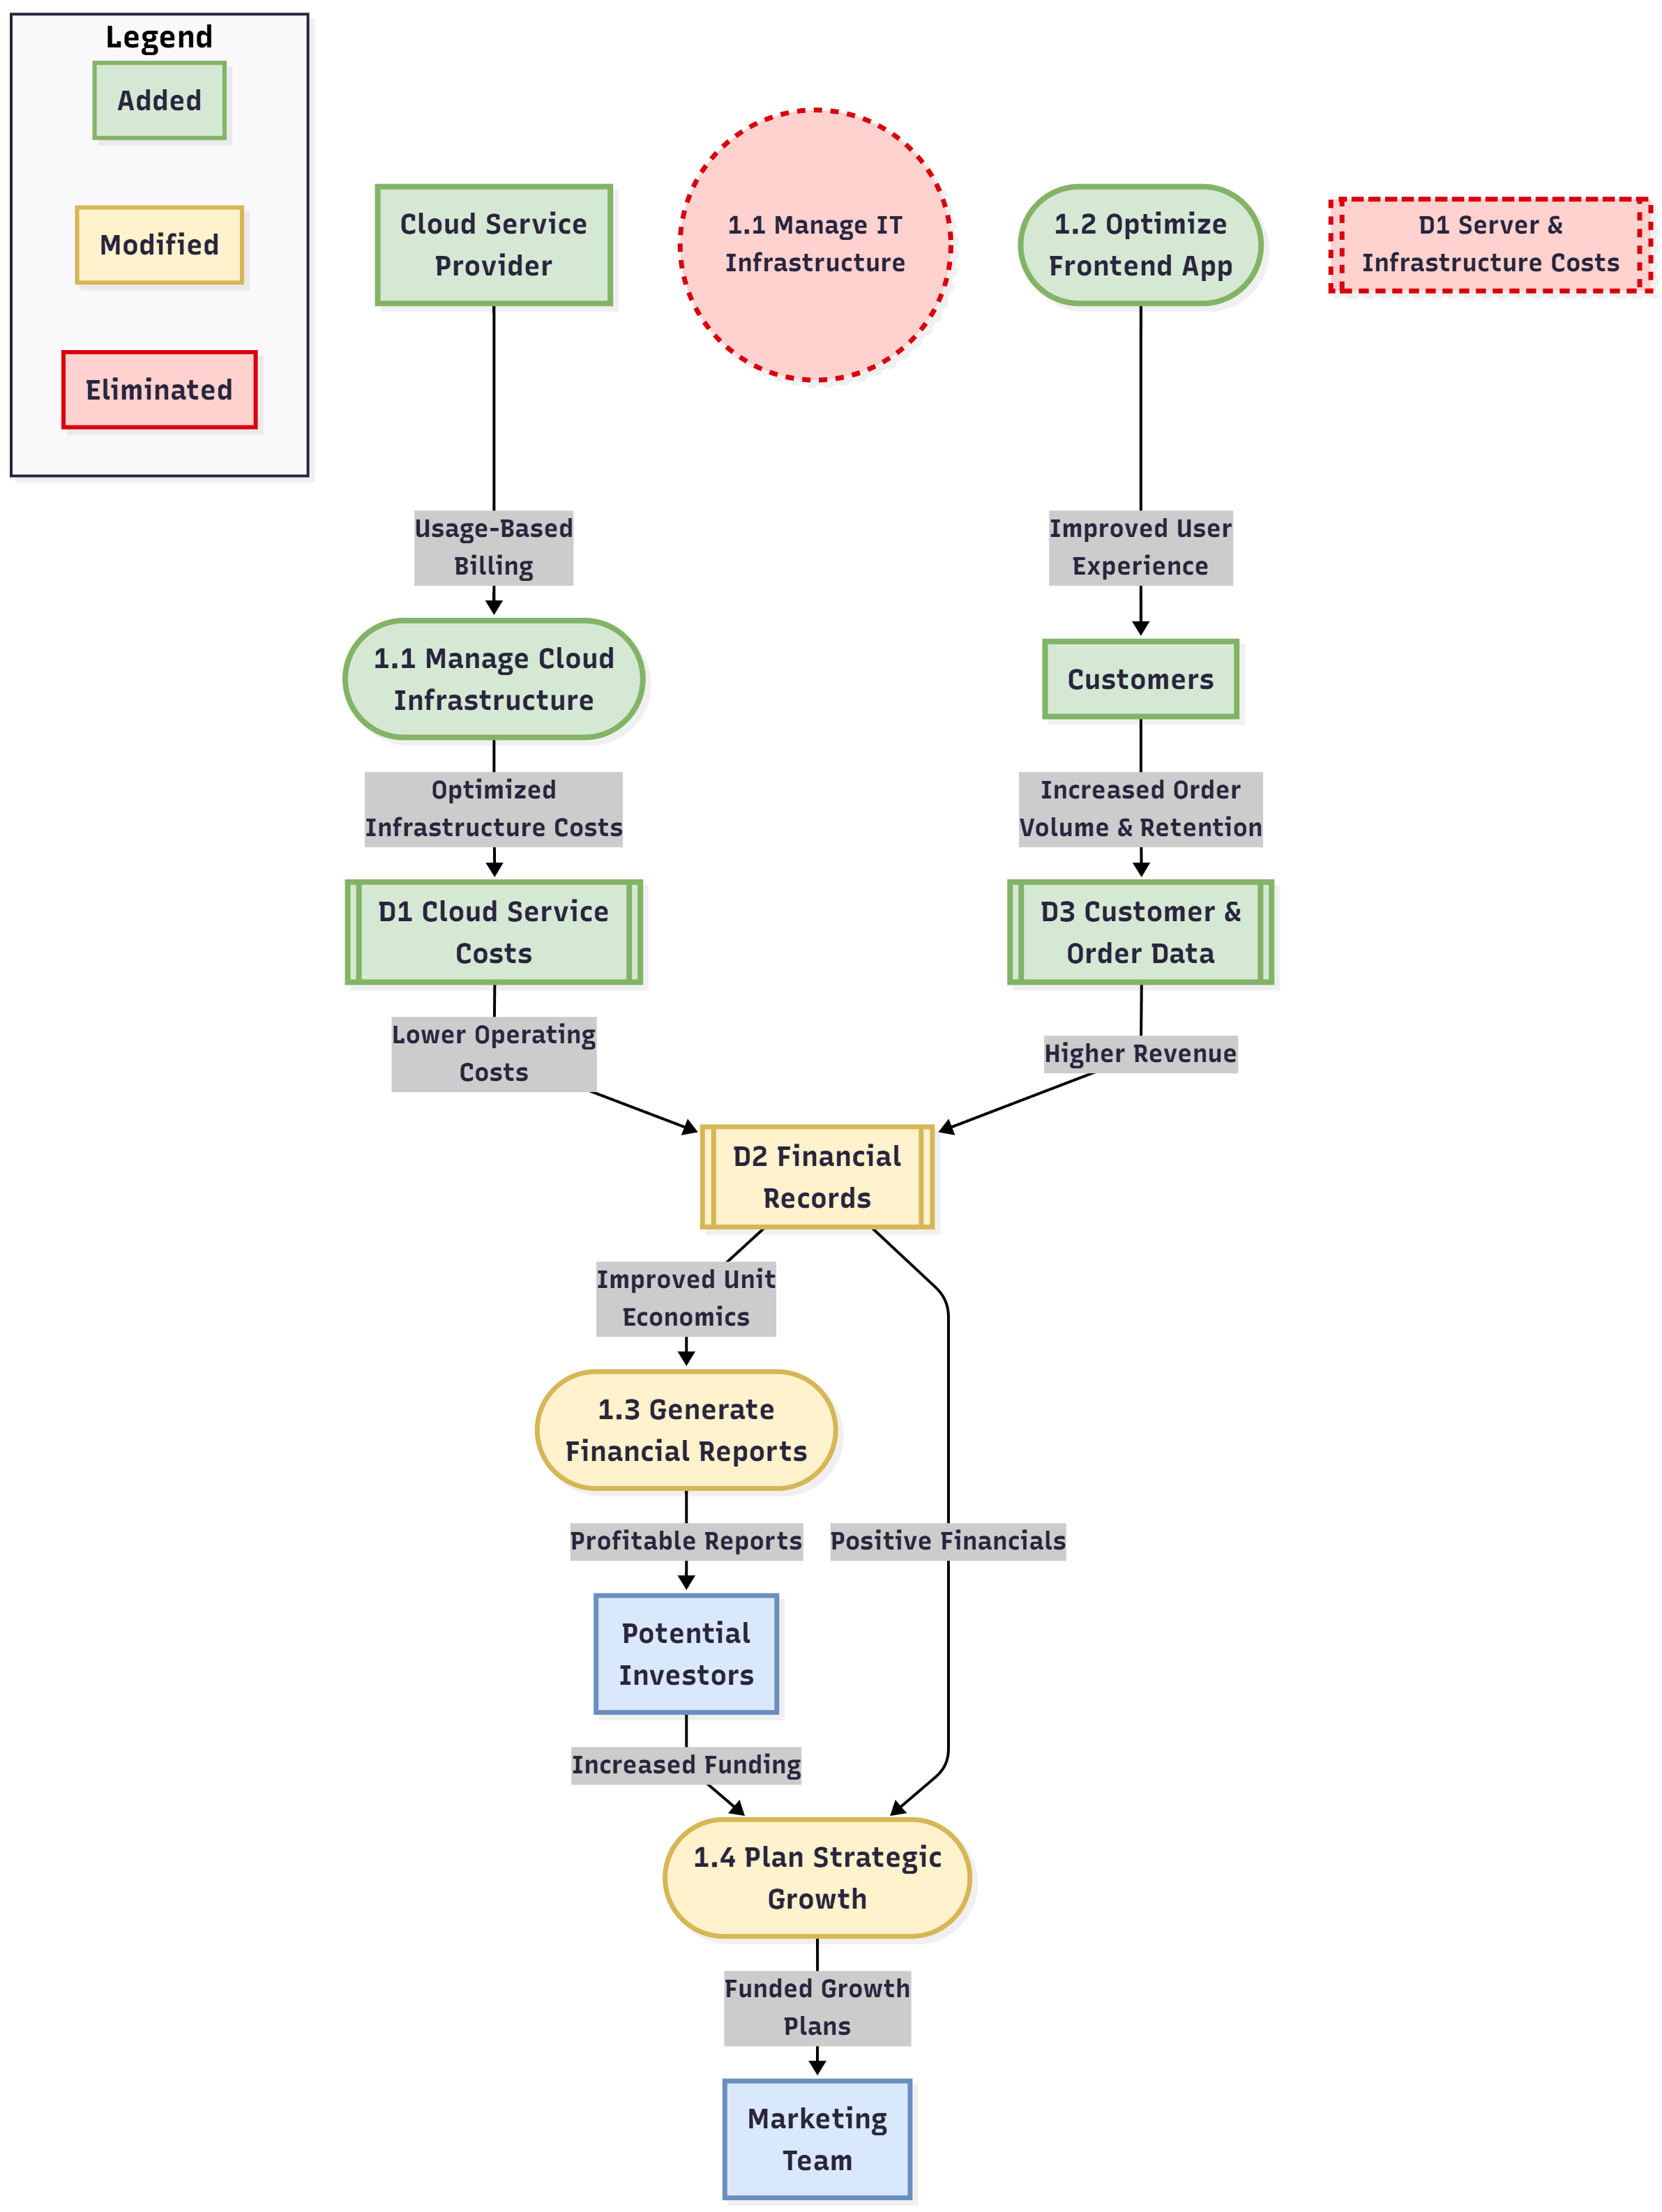
\includegraphics[width=1\textwidth]{new_dfd/problem1_3.png}
    \caption{Proposed DFD for problem 01}
    \label{fig:problem01}
\end{figure}

\begin{tcolorbox}[colback=green!5!white,colframe=green!75!black]
\begin{itemize}
    \item \textbf{1.2 Optimize Frontend App (Process):} A new, dedicated process focused on enhancing the user experience of the mobile app to drive customer satisfaction and retention.
    \item \textbf{D1 Cloud Service Costs (Data Store):} Replaces the old "Server \& Infrastructure Costs" store. It holds data on \textbf{Optimized Infrastructure Costs} which are variable and directly tied to usage, rather than fixed and high.
    \item \textbf{D3 Customer \& Order Data (Data Store):} A new data store to reflect the \textbf{Increased Order Volume \& Retention} driven by the improved app, feeding \textbf{Higher Revenue} data into the financial records.
\end{itemize}
\end{tcolorbox}

\subsubsection{Components Modified}
\begin{tcolorbox}[colback=yellow!5!white,colframe=yellow!75!black,title=Modified]
\begin{itemize}
    \item \textbf{1.3 Generate Financial Reports (Process):} This process is fundamentally modified. Instead of processing high costs and low revenue, it now receives \textbf{Lower Operating Costs} and \textbf{Higher Revenue}, allowing it to generate \textbf{Profitable Reports} that demonstrate positive \textbf{Improved Unit Economics}
    \item \textbf{1.4 Plan Strategic Growth (Process):} This process is transformed from a constrained function into an active one. Fueled by \textbf{Increased Funding} from investors and \textbf{Positive Financials}, it can now create actionable \textbf{Funded Growth Plans} for the marketing team.
   \item \textbf{D2 Financial Records (Data Store):} This data store is modified to reflect the new financial reality: a healthier balance sheet with significantly lower costs and higher, more predictable revenue streams.
\end{itemize}
\end{tcolorbox}

\subsubsection{Removed Components}
\begin{tcolorbox}[colback=red!5!white,colframe=red!75!black,title=Eliminated]
\begin{itemize}
    \item \textbf{Implicit High-Cost Server Maintenance::} While not shown as a formal process in the original DFD, the high cost and effort of maintaining on-premise servers have been eliminated and replaced by the more efficient 1.1 Manage Cloud Infrastructure process. This is the single most important change for improving Chaldal's profitability.
    \item \textbf{1.1 Manage IT Infrastructure (Process):} The previous, inefficient process of maintaining over-engineered, on-premise servers is completely removed. Its high maintenance effort and costs are now gone.
    \item \textbf{D1 Server \& Infrastructure Costs (Data Store):} This data store, which represented a major financial drain on the company, has been eliminated and replaced by the lean \textbf{Cloud Service Costs} store.
\end{itemize}
\end{tcolorbox}

\subsubsection{How This Solves the Problem}
This proposed system directly solves the Lack of Profitability and Funding Constraints in two ways:
\begin{itemize}[leftmargin=*]
  \item \textbf{It Attacks Costs:} By eliminating the expensive on-premise servers and their high maintenance overhead (\textbf{P1\_eliminated}), the single largest contributor to the company's unprofitability is removed. The new cloud model (\textbf{P1\_added}) reduces operational costs and makes them scalable with demand.
  \item \textbf{It Boosts Revenue:} By focusing on optimizing the mobile app (\textbf{P1\_app}), the system improves the primary customer touchpoint. A better, faster app leads to higher customer retention and increased order frequency (\textbf{D3}), directly increasing the company's revenue.
\end{itemize}
This combination of lower costs and higher revenue transforms the company's financial statements from unprofitable to profitable. These positive results (\textbf{Profitable Reports}) restore investor confidence, solving the funding constraint (\textbf{Increased Funding}) and allowing the company to break the cycle of stagnation and invest in growth (\textbf{Funded Growth Plans}).

\subsubsection{Impact Analysis}
The implementation of this system is projected to have the following measurable impacts on key business metrics:

\begin{itemize}
    \item \textbf{Operational Cost Reduction:} IT operational costs are projected to decrease by 40-50\% annually, resulting in a direct saving of approximately 1,00,00,000 BDT per year.
    \item \textbf{Customer Retention and Revenue:} The optimized mobile app is projected to increase the customer retention rate by 10\%, translating into an estimated 40,00,000 BDT in additional annual revenue.
    \item \textbf{Key Financial Metrics:} The project is expected to reach its break-even point in just 1.05 years, after which it will generate a net annual benefit of 95,00,000 BDT.
    \item \textbf{Application Performance:} User experience metrics are expected to improve significantly, with a target to reduce the application crash rate from 10\% to under 2\% and decrease average page load times by 50\%.
\end{itemize}

\subsubsection{Case Study}

\textbf{Netflix's Migration to the Cloud:} In 2008, Netflix experienced a major database corruption that halted DVD shipments for three days, highlighting the risk of relying on a single, on-premise data center. This event triggered a multi-year migration to a highly reliable, scalable cloud infrastructure provided by Amazon Web Services (AWS). By moving to the cloud, Netflix transformed its business. It no longer had to worry about managing physical servers and could instead focus its engineering talent on its core competency: improving the streaming experience. The cloud allowed Netflix to scale its services globally at a massive rate, handle huge fluctuations in demand, and deploy new features rapidly. This strategic shift away from owned infrastructure was a critical enabler of its growth from a US-based DVD service to a global streaming giant, demonstrating how a "lean IT" approach directly fuels profitability and business expansion.

% Problem 02: Product Sourcing and Supply Chain Inefficiencies
\subsection{Addressing Problem 02: Product Sourcing and Supply Chain Inefficiencies}

\subsubsection{Summary}

This Data Flow Diagram outlines a modernized, proactive, and data-driven supply chain system for Chaldal. It replaces the previous reactive and manual procurement process with an automated, integrated platform. The new system leverages a vendor portal for seamless communication, uses demand forecasting to automate purchasing, and implements a formal process for managing vendor performance and monitoring the cold chain. The result is a more reliable, efficient, and transparent supply chain that delivers higher quality products to customers.

\subsubsection{Components Added}
\begin{tcolorbox}[colback=green!5!white,colframe=green!75!black,title=New Components]
\begin{itemize}
    \item \textbf{Vendor Portal (External Entity):} A new digital interface for suppliers. Through this portal, vendors provide Real-time Stock Levels and Quality Reports, and receive Automated Purchase Orders, streamlining communication.
    \item \textbf{2.1 Automated Procurement (Process):} This new "PROACTIVE" process replaces reactive sourcing. It intelligently uses Forecast Data, Performance Data, and Real-time Stock Levels to optimize purchasing.
    \item \textbf{2.2 Manage Vendor Performance (Process):} A formal process where the Procurement Team conducts Vendor Audits. This process generates Vendor Scorecards and updates the list of certified suppliers.
    \item \textbf{2.3 Monitor Cold Chain (Process):} A dedicated process to track the temperature and conditions of perishable goods, sending Cold Chain Failure Reports to the performance management process.
    \item \textbf{D4 Vendor Performance Data (Data Store):} A new data store that holds objective metrics on vendor reliability, quality, and timeliness, enabling data-driven sourcing decisions.
    \item \textbf{D5 Demand Forecasts (Data Store):} A new data store that uses historical sales data and predictive analytics to forecast future product demand, driving the automated procurement process.
\end{itemize}
\end{tcolorbox}

\subsubsection{Components Modified}
\begin{tcolorbox}[colback=yellow!5!white,colframe=yellow!75!black,title=Modified]
\begin{itemize}
    \item \textbf{D1 Vendor \& Contract Data (Data Store):} Modified from a simple database to a comprehensive store containing Certified Vendor Info and contractual agreements, which is now actively used to select suppliers.
    \item \textbf{D2 Inventory Records (Data Store):} This store is now updated with Accurate Stock Updates of high-quality products, leading to a much more Reliable Inventory Status for fulfilling orders.
    \item \textbf{D3 Quality \& Spoilage Data (Data Store):} Now receives structured Spoilage \& Quality Updates from the performance management process, providing more accurate insights.
    \item \textbf{2.4 Update Inventory \& 2.5 Fulfill Customer Orders (Processes):} These processes are significantly improved. They now handle High-Quality Products and operate with reliable inventory data, resulting in the delivery of Consistent \& Quality Orders to customers.
\end{itemize}
\end{tcolorbox}

\begin{figure}[H]
    \centering
    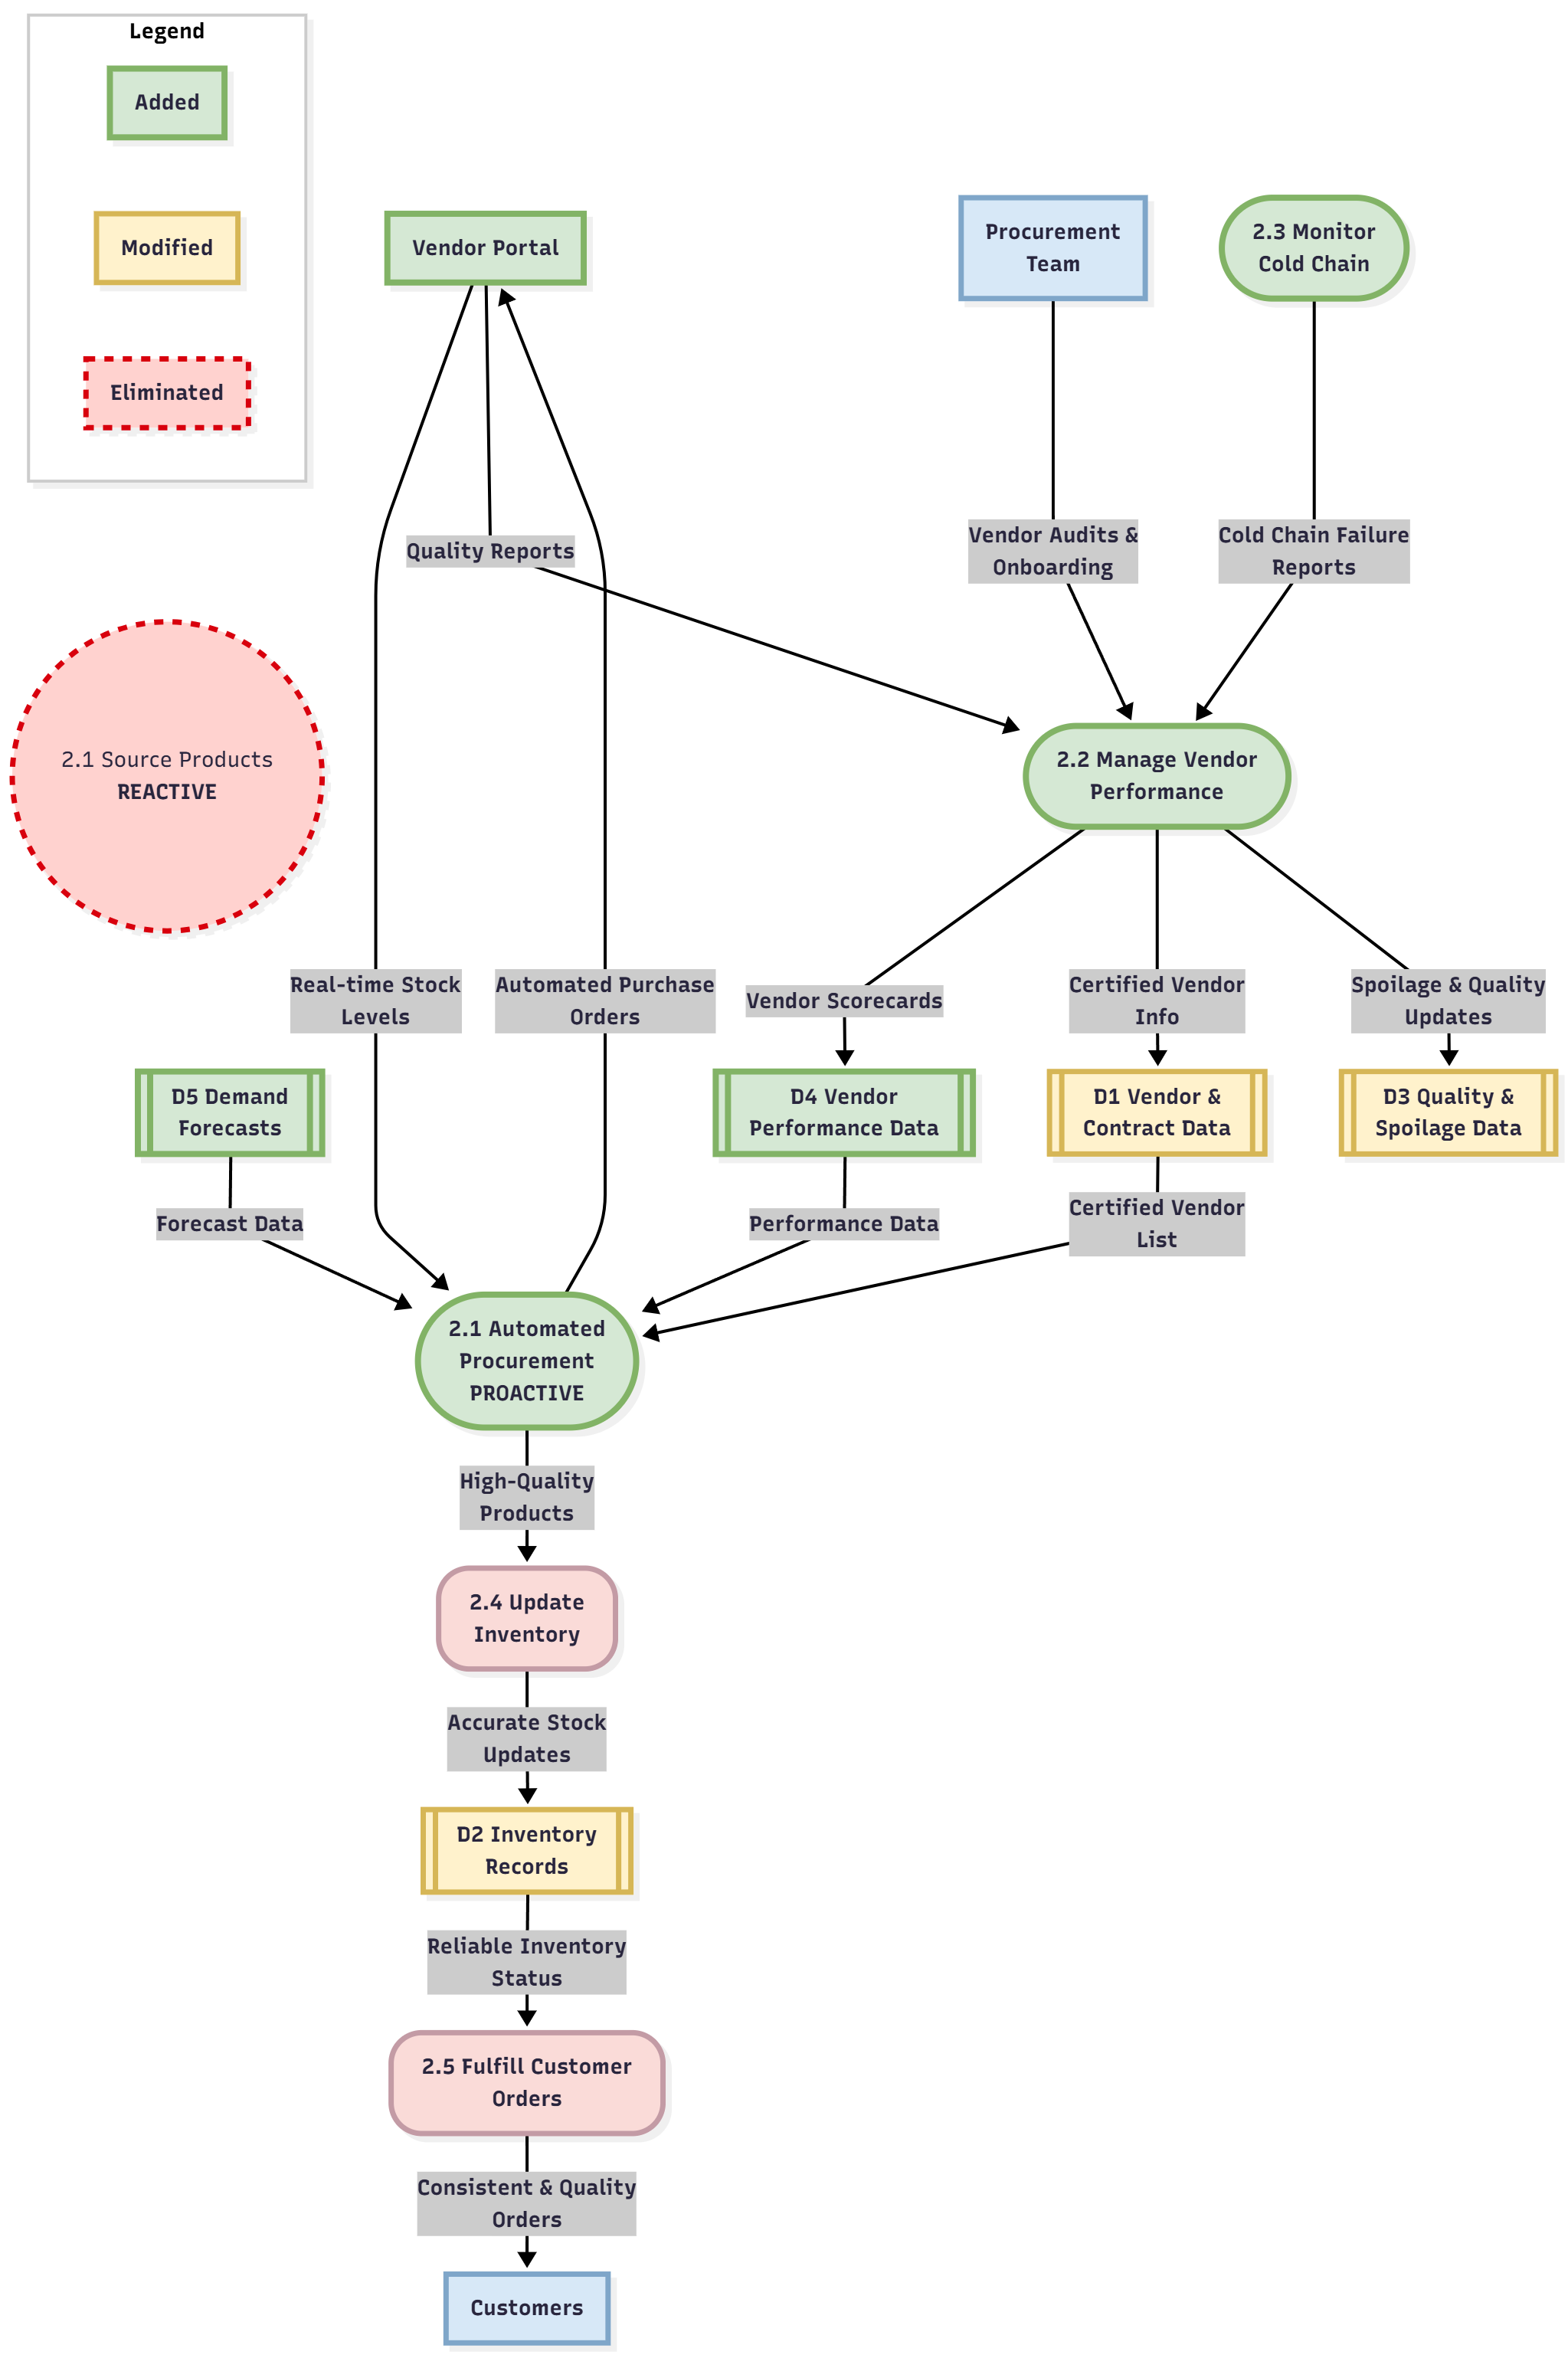
\includegraphics[width=1\textwidth]{new_dfd/problem2_2.png}
    \caption{Proposed DFD for problem 02}
    \label{fig:problem02}
\end{figure}



\subsubsection{Components Eliminated}
\begin{tcolorbox}[colback=red!5!white,colframe=red!75!black,title=Eliminated]
\begin{itemize}
    \item \textbf{2.1 Source Products REACTIVE (Process):} The old, inefficient, and manual sourcing process is completely eliminated. Its removal addresses the core bottleneck of unreliable supply and inconsistent quality.
\end{itemize}
\end{tcolorbox}

\subsubsection{How This Solves the Problem}
This proposed system directly solves the Supply Chain Inefficiencies and Product Sourcing Challenges by:
\begin{itemize}[leftmargin=*]
  \item \textbf{Combating Unreliability:} The Manage Vendor Performance process creates a feedback loop. Poor performance (e.g., low-quality reports, cold chain failures) results in low scores in D4 Vendor Performance Data, which the Automated Procurement process then uses to prioritize better-performing, certified vendors. This replaces unreliable sourcing with a data-driven meritocracy.
  \item \textbf{Reducing Spoilage and Quality Issues:} The Monitor Cold Chain process provides real-time oversight, while the Vendor Portal allows for structured quality reporting. This ensures that only high-quality, fresh products enter the inventory.
  \item \textbf{Preventing Stockouts:} The Automated Procurement process uses Demand Forecasts to order products proactively, preventing the stockouts that previously resulted from manual, reactive purchasing and ensuring consistent product availability for customers.
\end{itemize}

\subsubsection{Impact Analysis (Statistical Projections)}
The implementation of this system is projected to have the following measurable impacts on supply chain metrics:

\begin{itemize}
    \item \textbf{Reduction in Spoilage:} The spoilage rate for perishable goods is projected to decrease from 12\% to below 5\%, saving significant costs.
    \item \textbf{Improved Order Fulfillment:} The stockout rate for high-demand items is expected to fall from 15\% to less than 3\%, leading to a higher order fulfillment rate and increased customer satisfaction.
    \item \textbf{Procurement Efficiency:} Automation is expected to reduce the administrative time spent on procurement by 60\% and lower overall procurement costs by 10-15\% by eliminating middlemen and prioritizing cost-effective suppliers.
    \item \textbf{Vendor Performance:} The vendor on-time delivery rate is projected to increase to over 95\% due to performance monitoring and scorecards.
\end{itemize}

\subsubsection{Short Case Study}

\textbf{BigBasket (India):} As India's largest online grocer, BigBasket faced immense challenges in sourcing fresh produce from a fragmented agricultural sector. To solve this, they implemented a comprehensive vendor management and direct sourcing program. They established collection centers in rural areas to buy directly from thousands of farmers, bypassing multiple layers of middlemen. BigBasket provided farmers with demand forecasts, quality guidelines, and fair, transparent pricing through a digital platform. They also invested heavily in a temperature-controlled supply chain. This digital integration with their suppliers, similar to the proposed system for Chaldal, allowed them to reduce spoilage, ensure high-quality produce, and maintain stable pricing, which became a key competitive advantage in the crowded Indian e-grocery market.

% Problem 03:Ineffective Customer Representative & Delivery Operations
\subsection{Addressing Problem 03:Ineffective Customer Representative Delivery Operations}

\subsubsection{Summary}

This Data Flow Diagram illustrates how the implementation of System 3 (Cloud \& App Optimization) provides the financial stability and data intelligence required to fix Chaldal's delivery operations. The cost savings and revenue gains from the new IT infrastructure create a stable budget, which funds a professional, full-time rider workforce and an automated dispatch system. This new, data-driven operation results in efficient deliveries, secure payments, and a vastly improved customer service experience.

\begin{figure}[H]
    \centering
    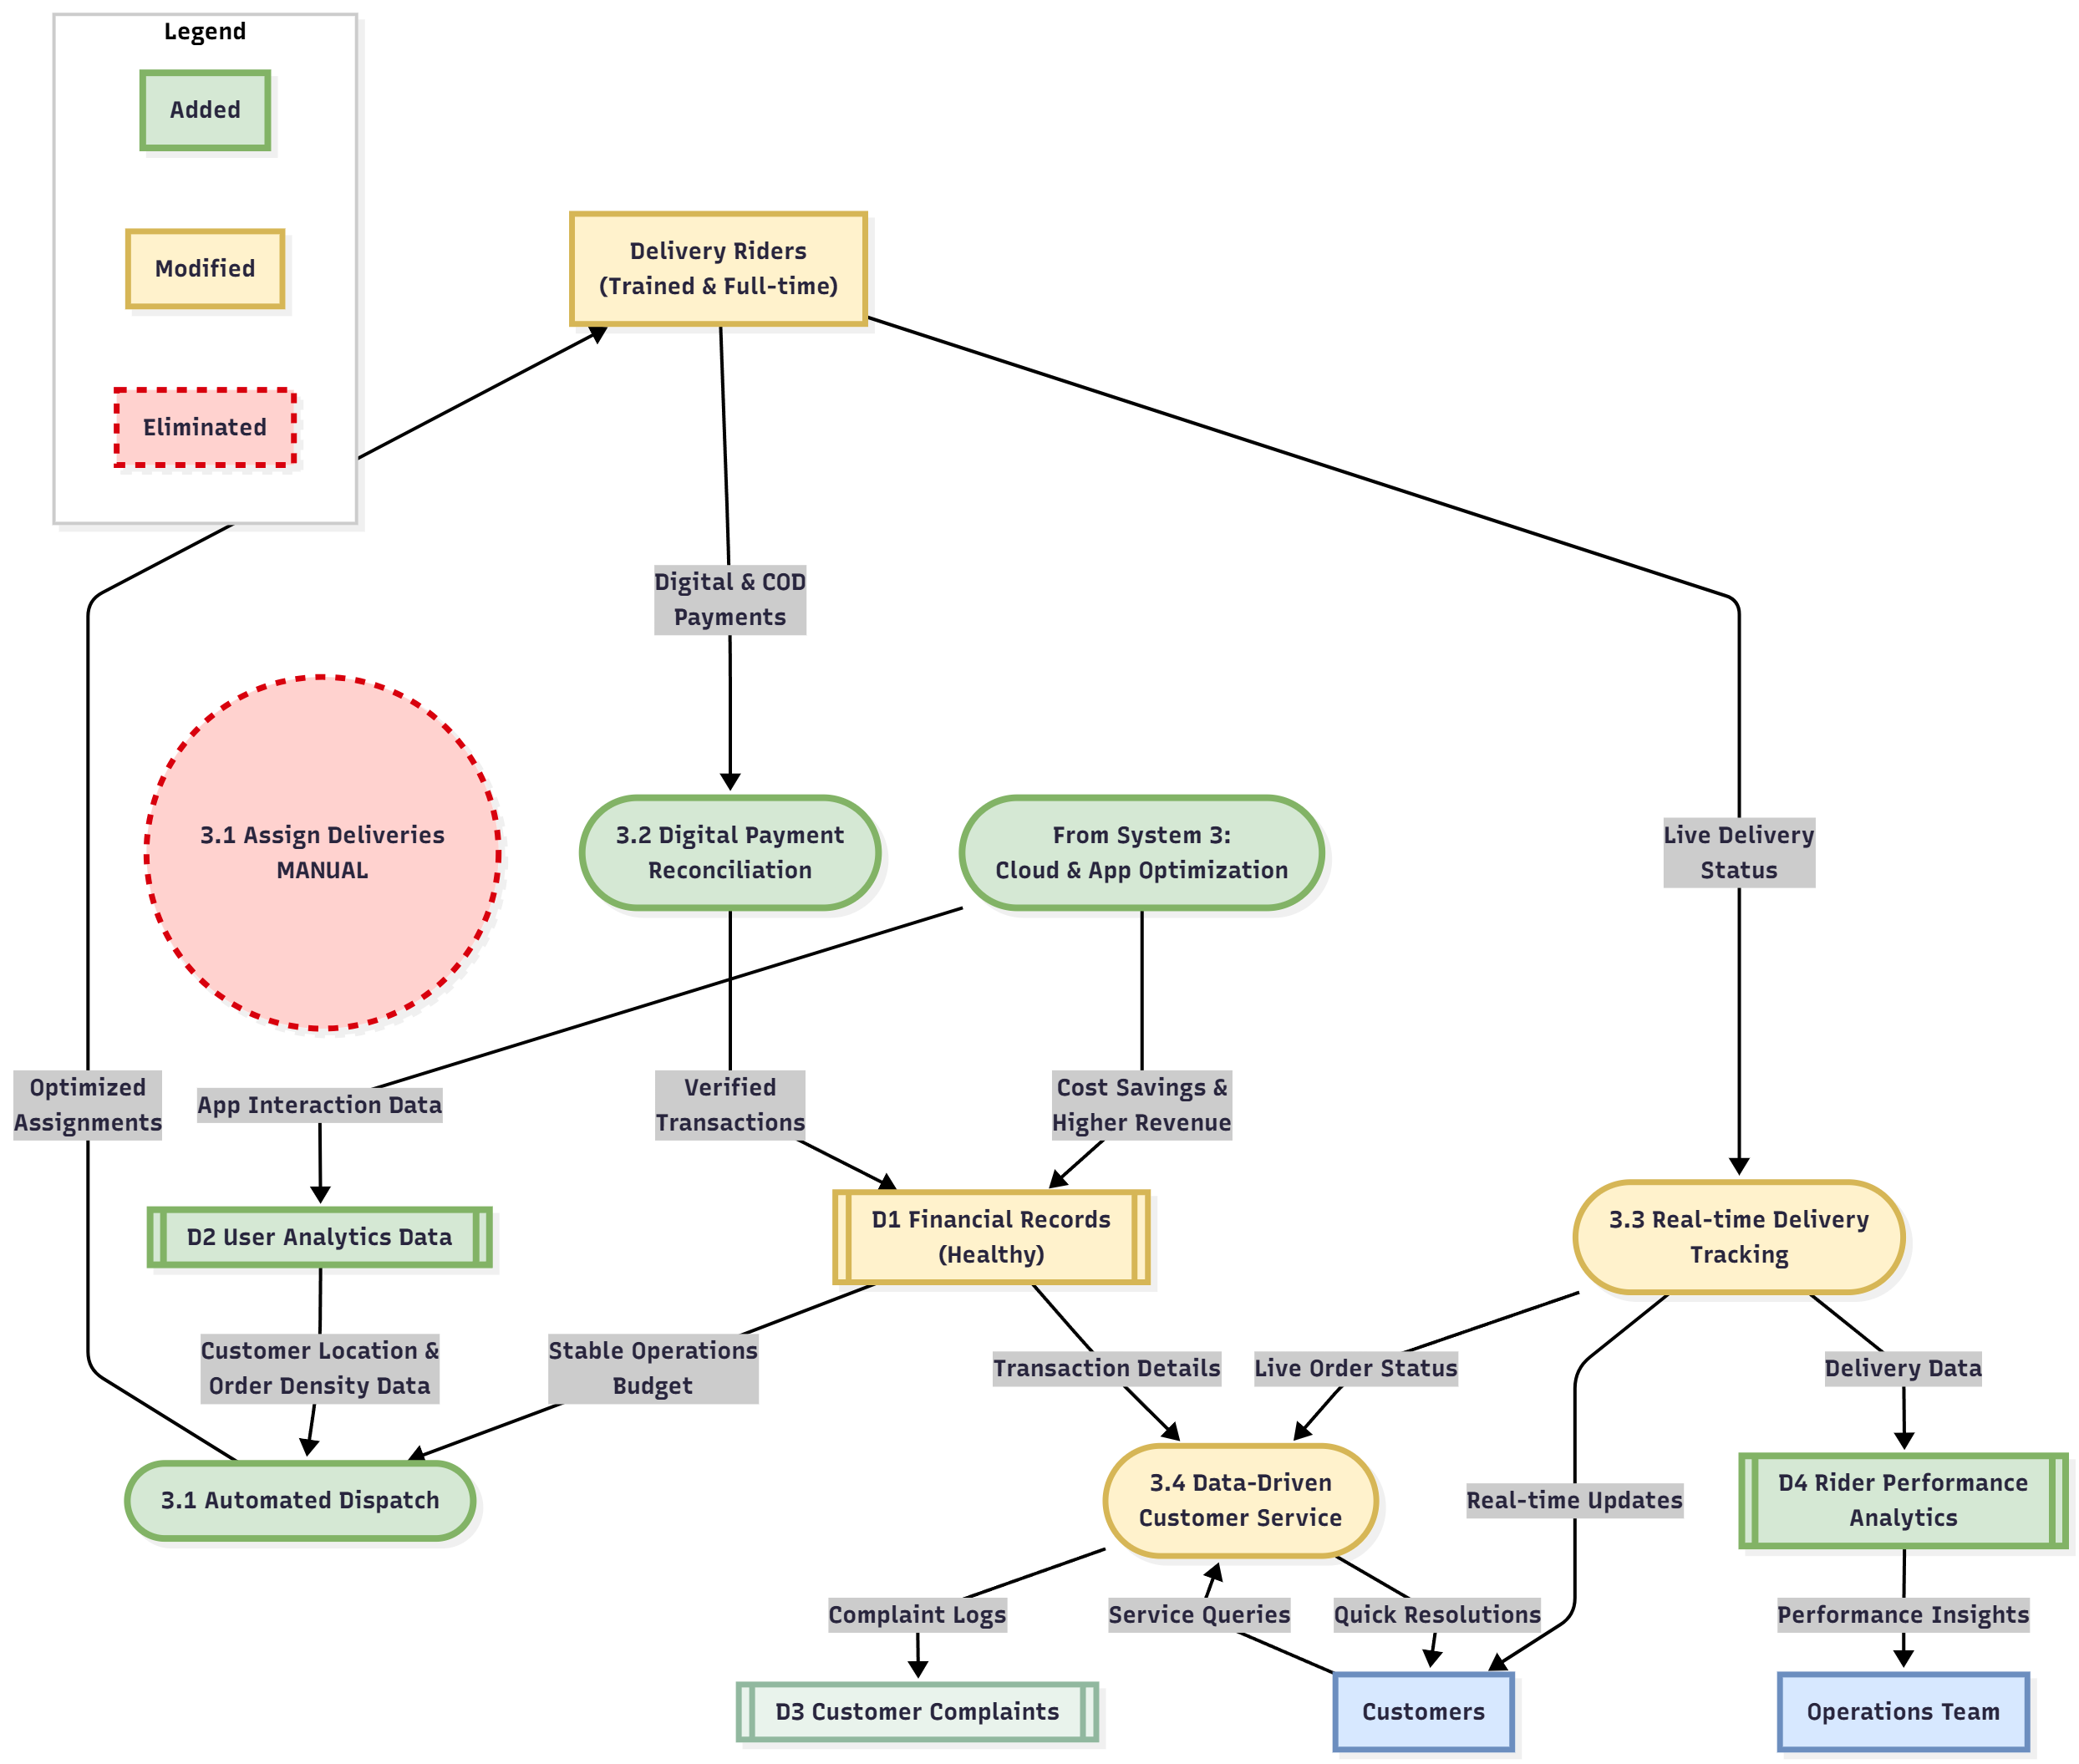
\includegraphics[width=1\textwidth]{new_dfd/problem3_3.png}
    \caption{Proposed DFD for problem 03}
    \label{fig:problem03}
\end{figure}

\subsubsection{Components Added}
\begin{tcolorbox}[colback=green!5!white,colframe=green!75!black,title=New Components]
\begin{itemize}
    \item \textbf{From System 3: Cloud \& App Optimization (Process):} This represents the foundational engine of change. It generates the Cost Savings \& Higher Revenue that make all other improvements possible. It also provides rich App Interaction Data.
    \item \textbf{3.1 Automated Dispatch (Process):} This new, intelligent process is now funded by the stable budget. It uses Customer Location \& Order Density Data from the optimized app to create efficient delivery routes.
    \item \textbf{3.2 Digital Payment Reconciliation (Process):} A new process, also funded by the new budget, to securely handle payments and reduce the risks of COD.
    \item \textbf{D2 User Analytics Data (Data Store):} This store captures data from the high-performing new app, providing valuable insights for logistics planning.
    \item \textbf{D4 Rider Performance Analytics (Data Store):} A new data store to track the performance of the professionalized rider fleet, enabling data-driven management.
\end{itemize}
\end{tcolorbox}

\subsubsection{Components Modified}
\begin{tcolorbox}[colback=yellow!5!white,colframe=yellow!75!black,title=Modified]
\begin{itemize}
    \item \textbf{Delivery Riders (Trained \& Full-time) (External Entity):} The workforce is transformed from unreliable part-timers to a professional, full-time team, made possible by the Stable Operations Budget.
    \item \textbf{D1 Financial Records (Healthy) (Data Store):} Modified to reflect a stable and positive financial state, which can now reliably fund operational needs like delivery.
    \item \textbf{3.3 Real-time Delivery Tracking \& 3.4 Data-Driven Customer Service (Processes):} These processes are now significantly more effective because they are supported by a professional rider team and have access to better data.
\end{itemize}
\end{tcolorbox}

\subsubsection{Components Eliminated}
\begin{tcolorbox}[colback=red!5!white,colframe=red!75!black,title=Eliminated]
\begin{itemize}
    \item \textbf{3.1 Assign Deliveries MANUAL (Process):} The inefficient, error-prone manual assignment process is eliminated, as the new budget allows for the implementation of a proper automated system.
\end{itemize}
\end{tcolorbox}

\subsubsection{How This Solves the Problem}
This system design solves the Ineffective Customer Representative \& Delivery Operations problem by first addressing its root cause: a lack of funding and stability.
\begin{itemize}[leftmargin=*]
  \item \textbf{System 3 provides the money:} The Cost Savings \& Higher Revenue create a Stable Operations Budget. This budget is the key that unlocks the solution.
  \item \textbf{The budget enables professionalization:} With stable funding, Chaldal can afford to hire Trained \& Full-time riders and invest in the technology for an Automated Dispatch system. This directly replaces the unreliable part-time workforce and inefficient manual assignments.
  \item \textbf{The new system improves service:} An automated dispatch, professional riders, and digital payment systems lead to faster, more reliable deliveries. This reduces the number of customer complaints and equips the customer service team with the real-time data needed to resolve issues quickly.
\end{itemize}

\subsubsection{Impact Analysis (Statistical Projections)}
The implementation of this system is projected to have the following measurable impacts on operational metrics:

\begin{itemize}
    \item \textbf{Delivery Efficiency:} Average dispatch and delivery time is projected to decrease by 25\%. The on-time delivery rate is expected to increase to over 95\%.
    \item \textbf{Financial Accuracy:} COD-related financial discrepancies are projected to decrease from 8\% to less than 1\%.
    \item \textbf{Workforce Stability:} Rider turnover is expected to decrease by 30-40\% due to the stability of full-time employment and fairer, data-driven performance management.
    \item \textbf{Customer Satisfaction:} The overall Customer Satisfaction Score (CSAT) is expected to improve by 10-15 points as delivery reliability becomes a core strength.
\end{itemize}

\subsubsection{Short Case Study}

\textbf{Domino's Pizza's Digital Transformation:} In the late 2000s, Domino's was struggling with a reputation for poor quality pizza and an outdated ordering system. They initiated a massive technological overhaul, branding themselves as a "tech company that sells pizza." They invested heavily in a new, user-friendly mobile app and online ordering platform (similar to Chaldal's System 3). The success of this digital platform generated a huge increase in sales and profits. Domino's then used this new financial strength and the data from their app to revolutionize their operations. They funded the development of GPS driver tracking, automated order assignments, and even experiments with drone delivery. The initial investment in their customer-facing tech (the app) directly enabled and paid for the complete modernization of their delivery logistics.


% Problem 04:Operational and HR Process Inefficiencies
\subsection{Addressing Problem 04:Operational and HR Process Inefficiencies}

\subsubsection{Summary}

This Data Flow Diagram shows the transformation of Chaldal's HR operations from a fragmented, manual, and error-prone system to a centralized, automated, and efficient one. The financial stability achieved through System 3 (Cloud \& App Optimization) provides the necessary budget to implement a modern Workforce Management System (WMS). This new system digitizes and integrates scheduling, leave requests, performance tracking, and payroll, which eliminates bottlenecks, improves transparency for employees, and provides managers with actionable data.

\begin{figure}[H]
    \centering
    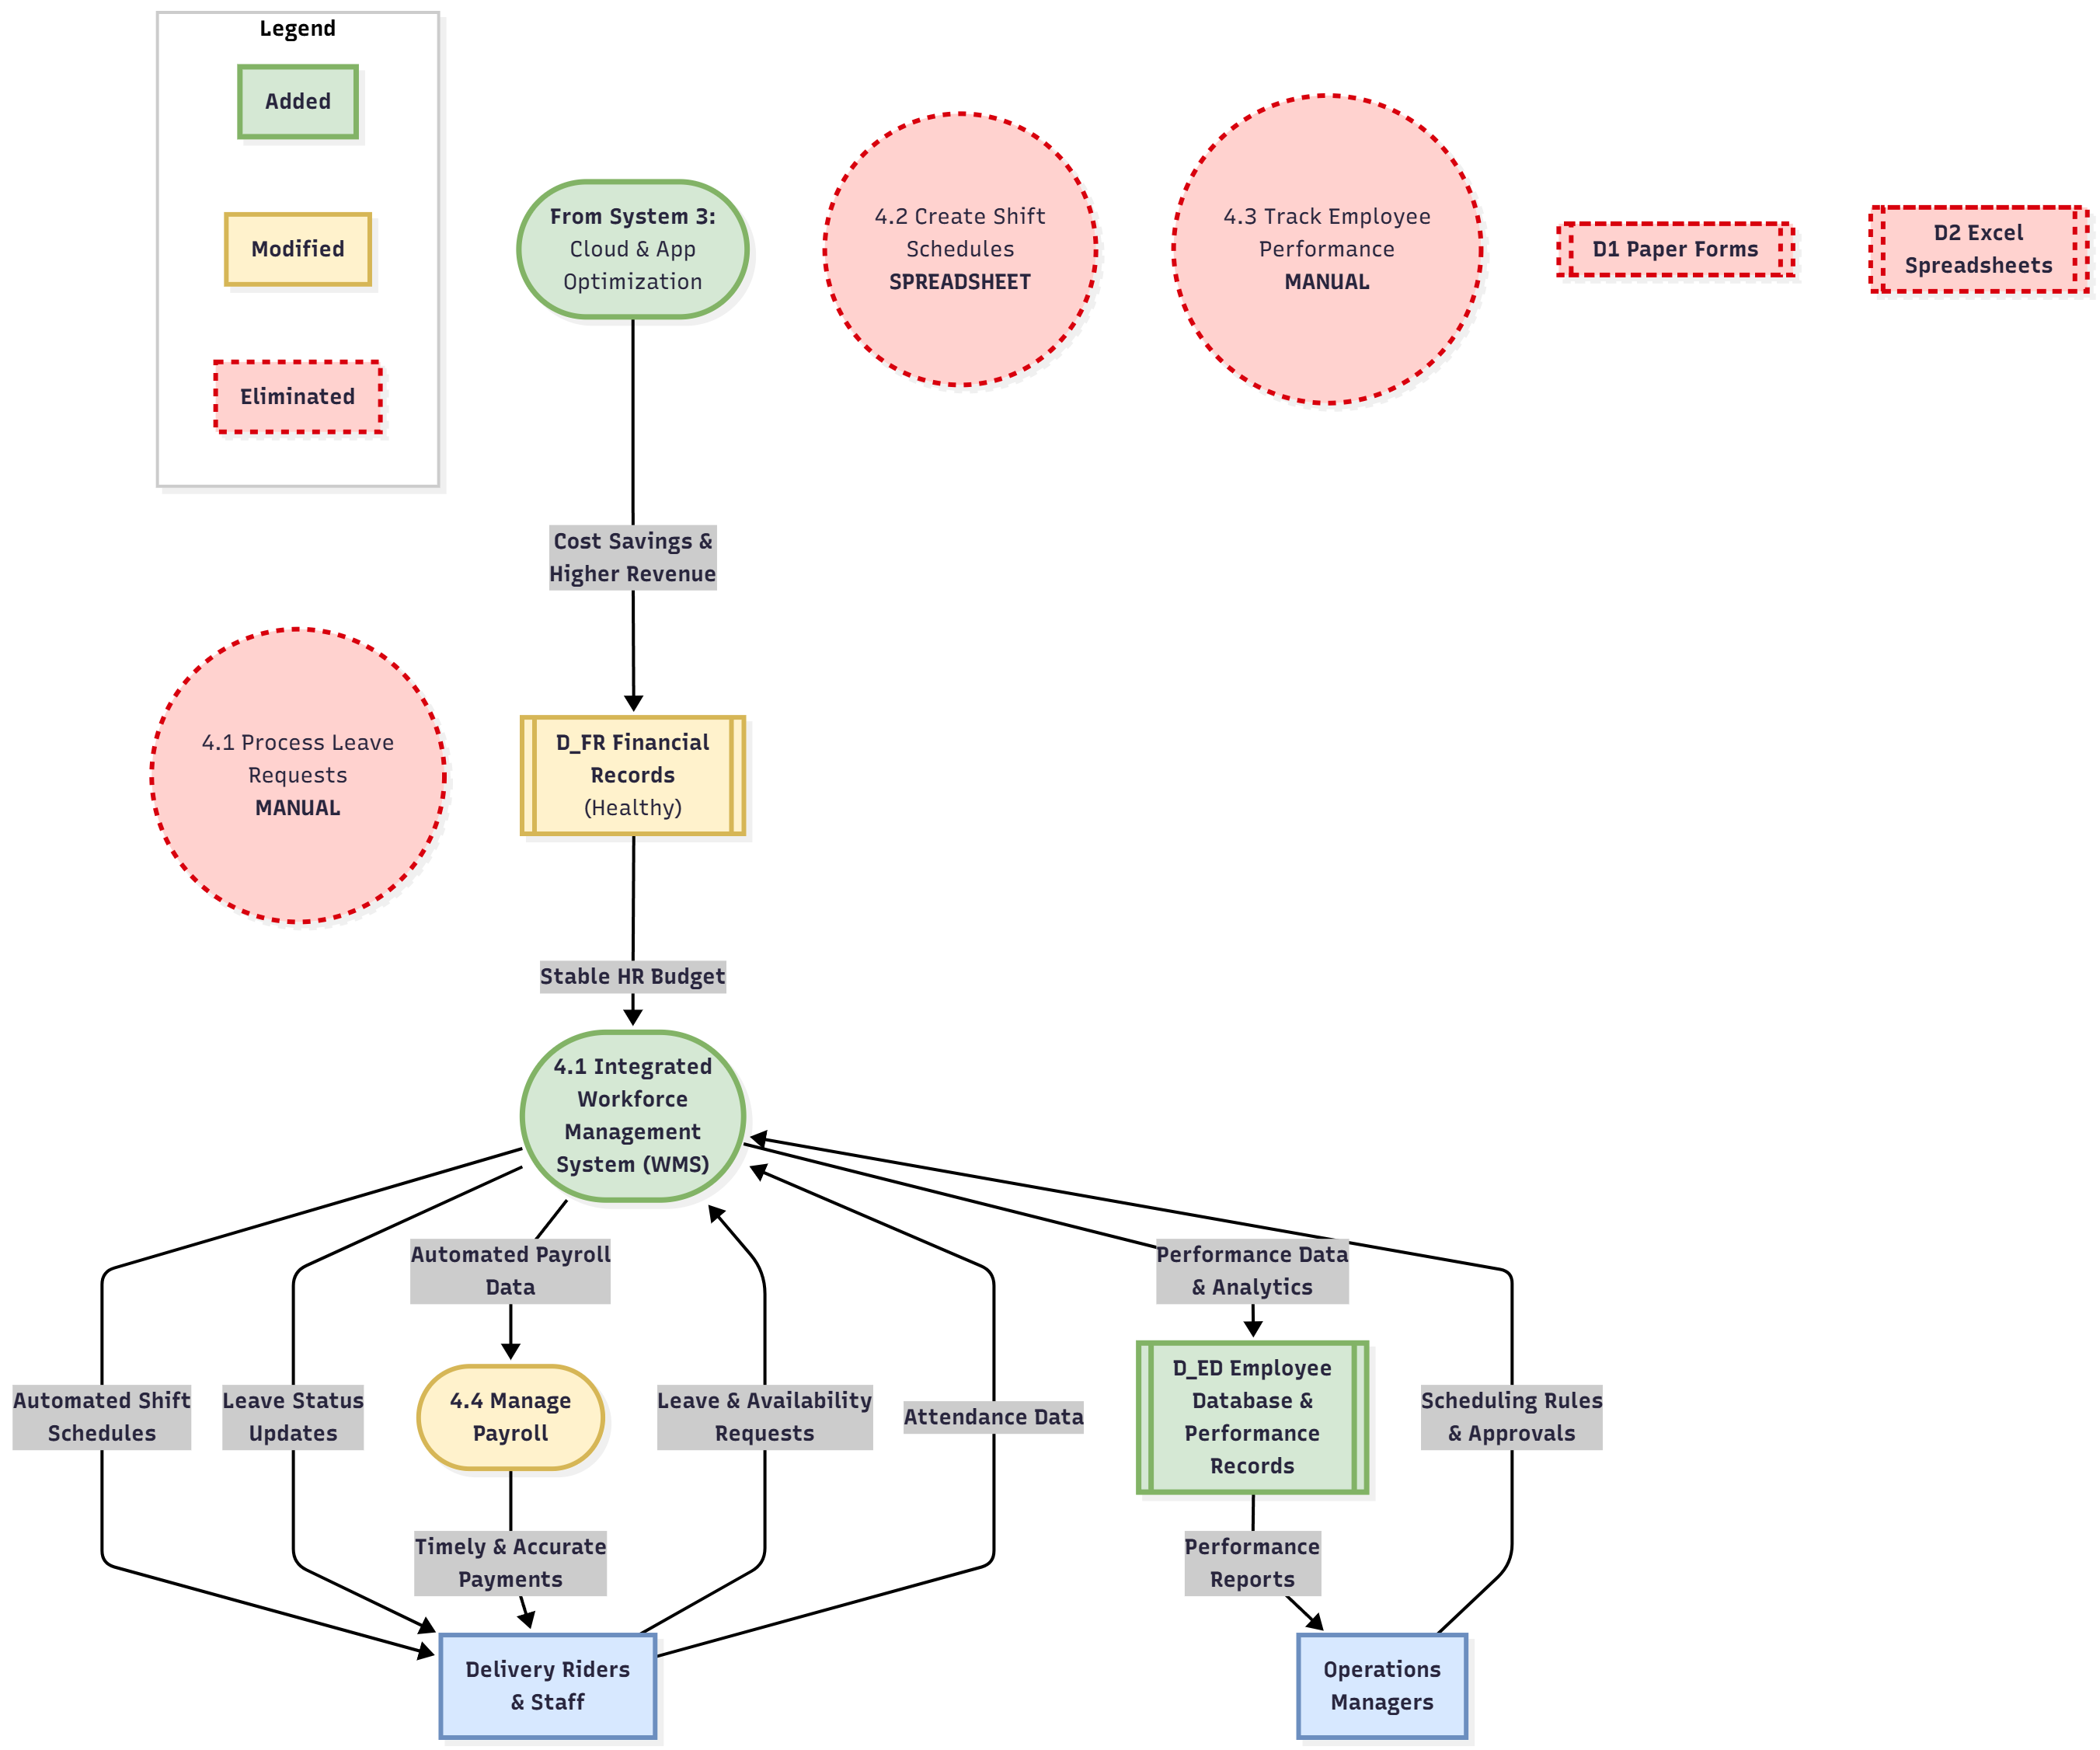
\includegraphics[width=1\textwidth]{new_dfd/problem4.png}
    \caption{Proposed DFD for Problem 04}
    \label{fig:problem04}
\end{figure}

\subsubsection{Components Added}
\begin{tcolorbox}[colback=green!5!white,colframe=green!75!black,title=New Components]
\begin{itemize}
    \item \textbf{From System 3: Cloud \& App Optimization (Process):} As the foundational enabler, this process generates the Cost Savings that create a Stable HR Budget, making investment in a proper HR system possible.
    \item \textbf{4.1 Integrated Workforce Management System (WMS) (Process):} This is the core of the new solution. It's a single, automated system that handles all key HR functions: processing Leave \& Availability Requests, creating Automated Shift Schedules, and tracking Performance Data.
    \item \textbf{D\_ED Employee Database \& Performance Records (Data Store):} A new, centralized database that replaces paper forms and spreadsheets. It securely stores all employee information and objective Performance Data \& Analytics generated by the WMS.
\end{itemize}
\end{tcolorbox}

\subsubsection{Components Modified}
\begin{tcolorbox}[colback=yellow!5!white,colframe=yellow!75!black,title=Modified]
\begin{itemize}
    \item \textbf{4.4 Manage Payroll (Process):} This process is significantly improved. Instead of relying on error-prone manual data from spreadsheets, it now receives Automated Payroll Data directly from the WMS, ensuring Timely \& Accurate Payments.
    \item \textbf{D\_FR Financial Records (Healthy) (Data Store):} This store is modified to reflect a healthy financial state, capable of allocating a stable budget to essential internal systems like HR.
\end{itemize}
\end{tcolorbox}

\subsubsection{Components Eliminated}
\begin{tcolorbox}[colback=red!5!white,colframe=red!75!black,title=Eliminated]
\begin{itemize}
    \item \textbf{Manual HR Processes (4.1, 4.2, 4.3):} All three of the old, manual processes (Process Leave Requests, Create Shift Schedules, Track Employee Performance) are made obsolete by the new integrated WMS and are therefore eliminated.
    \item \textbf{Paper and Spreadsheet Data Stores (D1, D2):} The inefficient and unreliable D1 Paper Forms and D2 Excel Spreadsheets are completely eliminated, replaced by the robust and secure digital Employee Database.
\end{itemize}
\end{tcolorbox}

\subsubsection{How This Solves the Problem}
This system design directly solves the Operational and HR Process Inefficiencies by:
\begin{itemize}[leftmargin=*]
  \item \textbf{Providing the Funding:} System 3 is the catalyst, creating a Stable HR Budget that allows Chaldal to move beyond makeshift solutions.
  \item \textbf{Centralizing and Automating:} The Integrated WMS replaces three separate, manual processes with one automated system. This eliminates the administrative burden, removes human error from scheduling, and gets rid of paperwork.
  \item \textbf{Creating Transparency and Fairness:} Employees interact with a consistent digital system for leave and scheduling, seeing Automated Shift Schedules and Leave Status Updates. This removes the perception of favoritism and builds trust.
  \item \textbf{Enabling Data-Driven Management:} The system captures objective performance data, allowing Operations Managers to make informed decisions based on Performance Reports instead of subjective evaluations. This leads to fairer assessments and more effective workforce management.
\end{itemize}

\subsubsection{Impact Analysis (Statistical Projections)}
The implementation of this system is projected to have the following measurable impacts on HR and operational metrics:

\begin{itemize}
    \item \textbf{Administrative Efficiency:} Time spent by managers on manual scheduling and HR administration is projected to decrease by 75\%.
    \item \textbf{Scheduling Accuracy:} Scheduling errors that lead to understaffing or overbooking are expected to decrease from 10\% of shifts to less than 1\%.
    \item \textbf{Payroll Accuracy:} Payroll errors requiring manual correction are projected to decrease by over 90\%, improving employee satisfaction and trust.
    \item \textbf{Employee Turnover:} High turnover, partly attributed to HR issues, is expected to decrease by 15-20\% as transparency, fairness, and payment reliability improve.
\end{itemize}

\subsubsection{Short Case Study}

\textbf{Starbucks' Workforce Management:} With thousands of stores and baristas working variable hours, Starbucks faced a massive scheduling challenge. They moved from manual, in-store scheduling to a centralized Workforce Management System. The new system, called "Teamworks," uses data to forecast customer traffic and automatically generates optimized schedules for each store. Baristas can now use a mobile app to view their schedules, swap shifts, and request time off. This automation drastically reduced the time managers spent on administrative tasks, minimized scheduling errors, and gave employees more flexibility and control over their work lives. It solved the core inefficiency and transparency problems of their old manual system, improving both operational efficiency and employee morale on a global scale.

% Problem 05: Under-Optimized Application and Over-Engineered IT Infrastructure
\subsection{Addressing Problem 05: Under-Optimized Application and Over-Engineered IT Infrastructure}

\subsubsection{Summary}

This Data Flow Diagram illustrates the strategic realignment of Chaldal's technology division. It shows a shift from a dysfunctional, high-cost model with misaligned priorities to a lean, efficient, and user-centric operation. The new system eliminates costly server maintenance and a resource-starved frontend team, replacing them with a single, refocused engineering process that manages a cost-effective cloud infrastructure and delivers a high-performance mobile application. This creates a positive feedback loop where a better app drives user engagement, which is supported by a scalable and affordable backend.

\subsubsection{Components Added}
\begin{tcolorbox}[colback=green!5!white,colframe=green!75!black,title=New Components]
\begin{itemize}
    \item \textbf{Cloud Service Provider (External Entity):} Replaces the need for physical backend servers, providing a scalable, pay-as-you-go infrastructure.
    \item \textbf{5.3 Manage Lean Infrastructure \& App Development (Process):} This new, unified process is the core of the solution. It represents the refocused engineering effort, now balanced between managing an efficient cloud backend and pushing Continuous App Improvements to the frontend.
    \item \textbf{D3 Cloud Monitoring \& Billing (Data Store):} A new data store that tracks cloud usage and costs, providing transparency and allowing for continuous cost optimization.
\end{itemize}
\end{tcolorbox}
\begin{figure}[H]
    \centering
    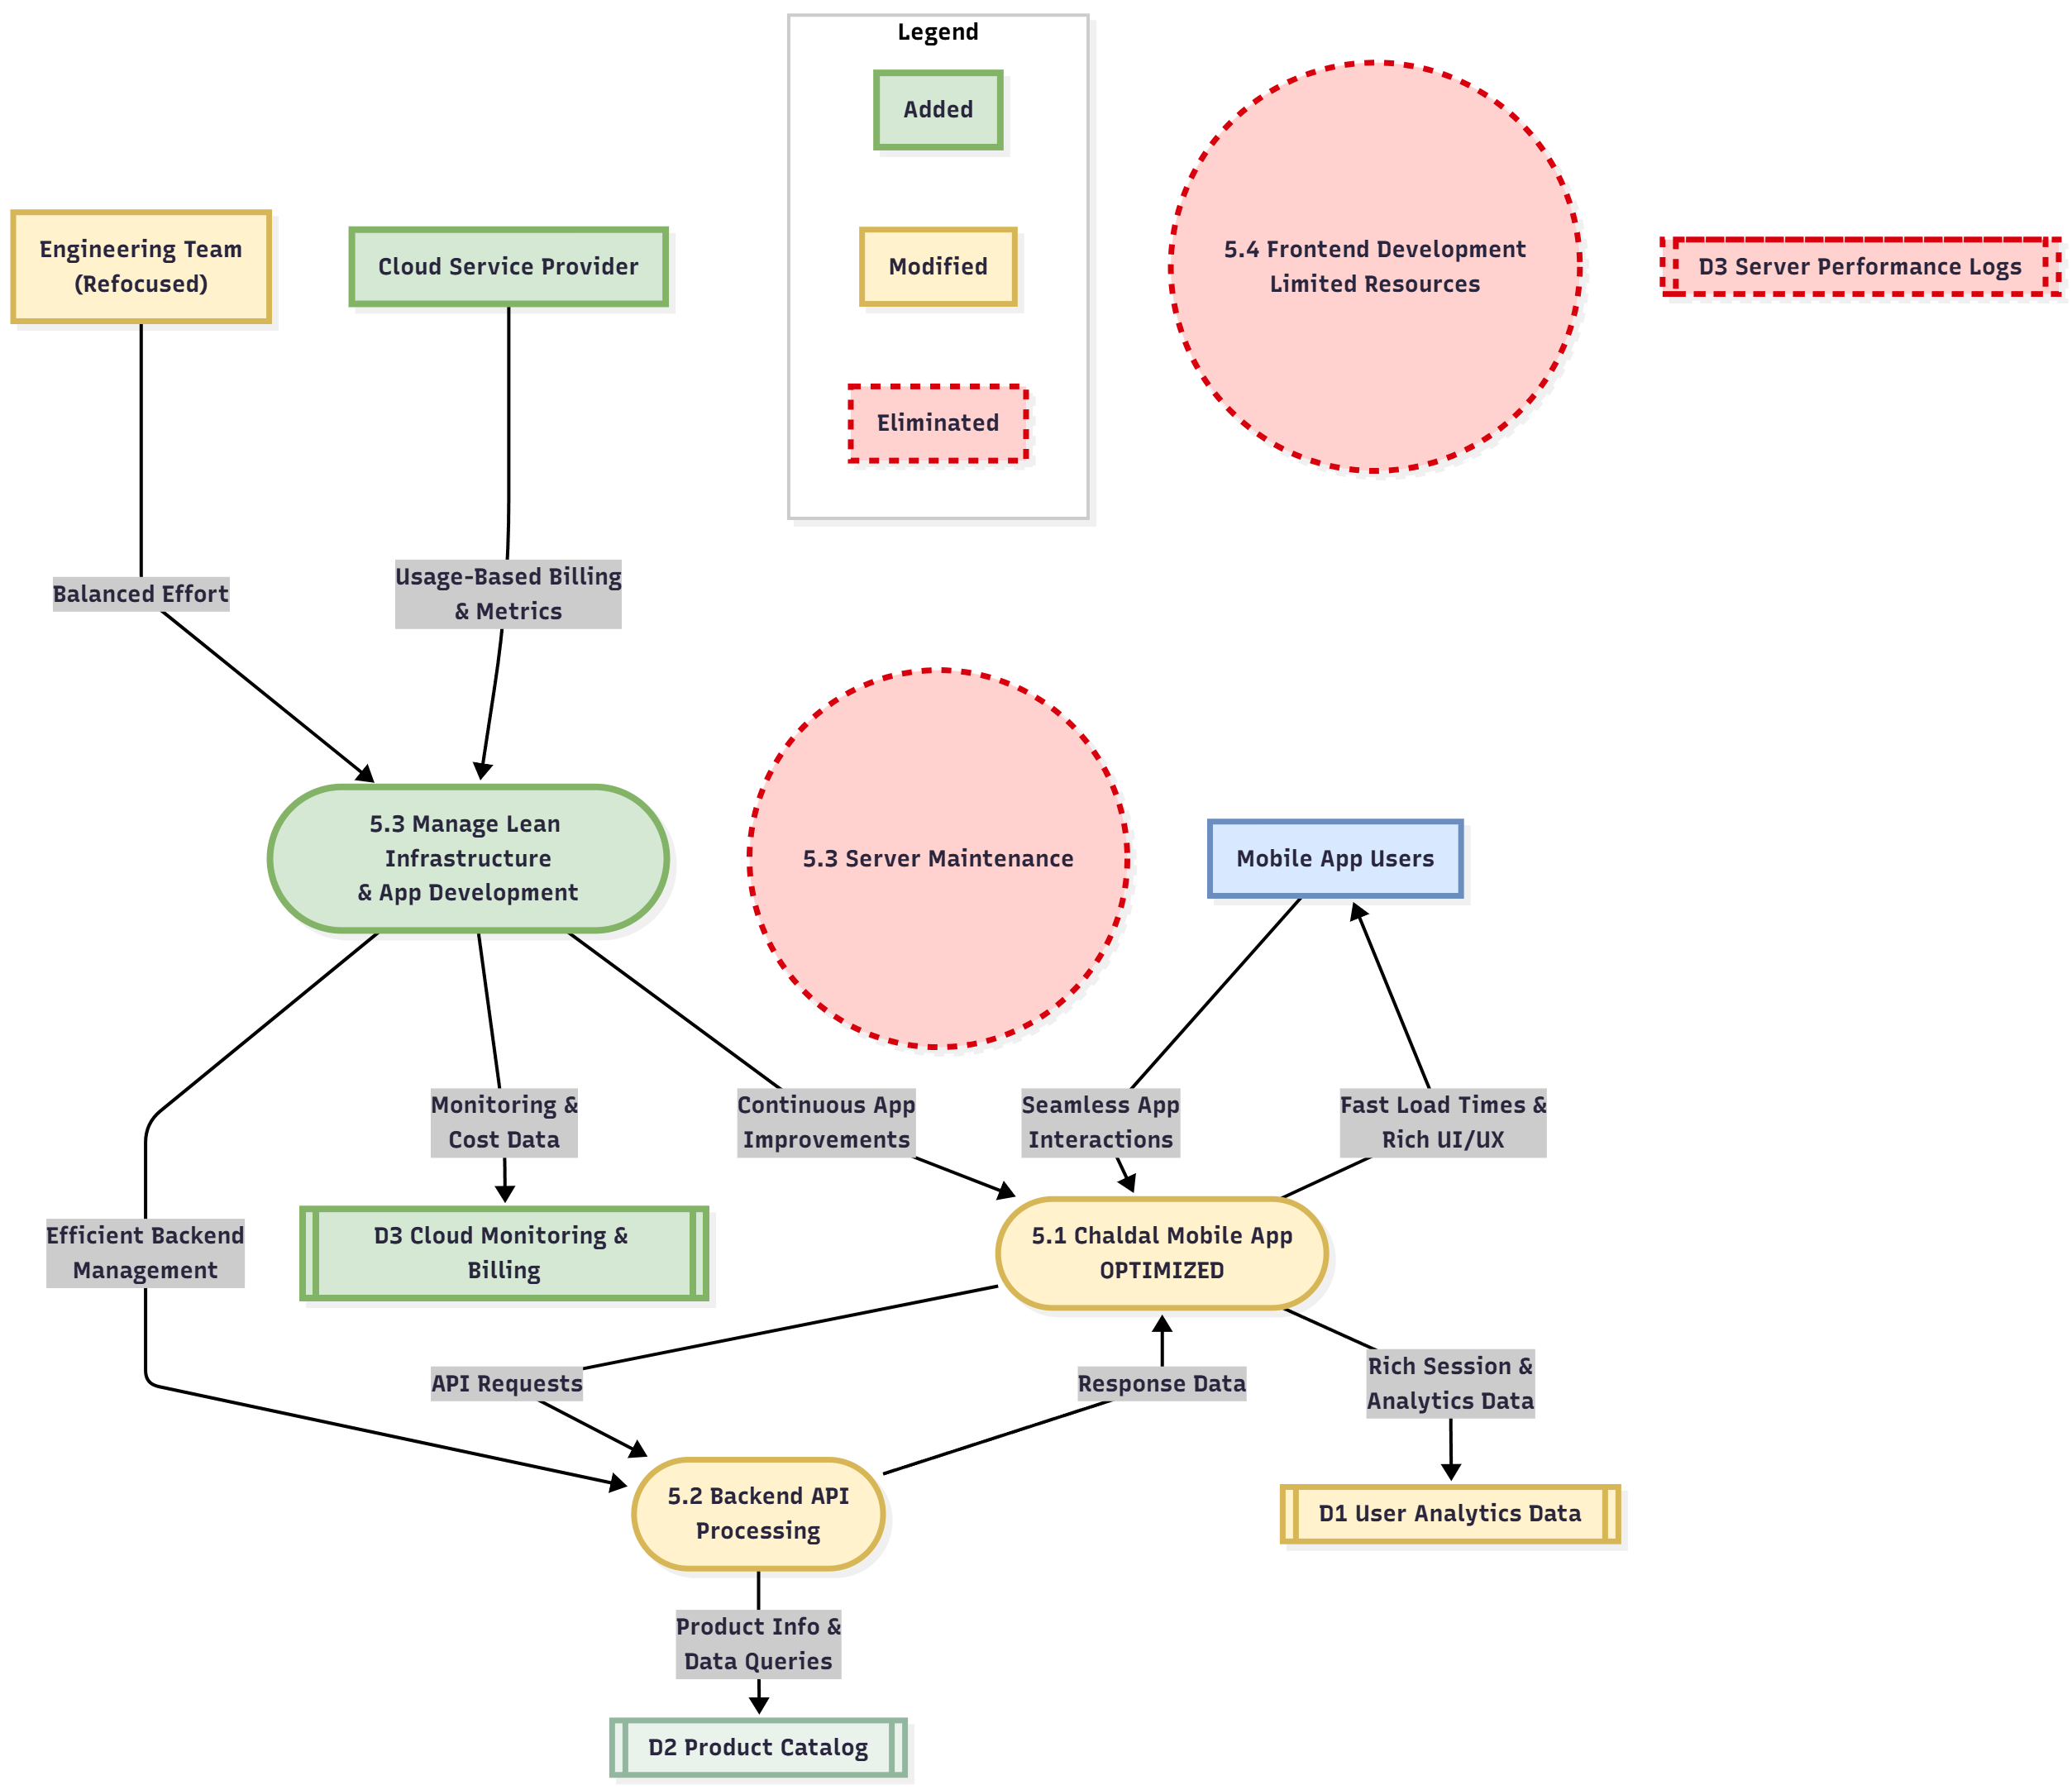
\includegraphics[width=1\textwidth]{new_dfd/problem5_1.png}
    \caption{Proposed DFD for Problem 05}
    \label{fig:problem05}
\end{figure}



\subsubsection{Components Modified}
\begin{tcolorbox}[colback=yellow!5!white,colframe=yellow!75!black,title=Modified]
\begin{itemize}
    \item \textbf{Engineering Team (Refocused) (External Entity):} The team's effort is modified from a 60/40 backend-heavy split to a Balanced Effort, allowing for proper attention to the user-facing application.
    \item \textbf{5.1 Chaldal Mobile App (OPTIMIZED) (Process):} The app is transformed from "UNDER-OPTIMIZED" to "OPTIMIZED." It now provides Fast Load Times \& Rich UI/UX to users and, in turn, captures more valuable Rich Session \& Analytics Data.
    \item \textbf{5.2 Backend API Processing (Process):} This process is modified to run on a lean, efficient cloud infrastructure, making it more reliable and scalable without the high overhead.
    \item \textbf{D1 User Analytics Data (Data Store):} Modified from a simple session store to a rich analytics database that captures detailed user interactions from the high-performance app.
\end{itemize}
\end{tcolorbox}

\subsubsection{Components Eliminated}
\begin{tcolorbox}[colback=red!5!white,colframe=red!75!black,title=Eliminated]
\begin{itemize}
    \item \textbf{5.3 Server Maintenance (Process):} The costly, time-consuming process of maintaining physical, on-premise servers is completely eliminated.
    \item \textbf{5.4 Frontend Development (Limited Resources) (Process):} The previous, under-staffed, and ineffective frontend effort is eliminated and absorbed into the new, properly resourced, unified development process.
    \item \textbf{D3 Server Performance Logs (Data Store):} The data store for tracking the old, inefficient servers is now obsolete and has been eliminated.
\end{itemize}
\end{tcolorbox}

\subsubsection{How This Solves the Problem}
This system design directly solves the Under-Optimized Application and Over-Engineered IT Infrastructure problem by:
\begin{itemize}[leftmargin=*]
  \item \textbf{Realigning Priorities:} It eliminates the two conflicting processes (Server Maintenance and Frontend Development) and replaces them with one unified process (Manage Lean Infrastructure \& App Development). This forces a balanced allocation of resources, solving the core issue of misaligned priorities.
  \item \textbf{Fixing the User Experience:} With a Balanced Effort from the engineering team, the mobile app receives the Continuous App Improvements it needs. This directly fixes the slow load times, poor UI/UX, and crashes that were alienating users. 3. Slashing Infrastructure Costs: By moving to a Cloud Service Provider, the massive, fixed cost of maintaining over-engineered servers is replaced with a variable, optimized cost structure. This directly addresses the financial drain and makes the IT operation financially sustainable.
\end{itemize}

\subsubsection{Impact Analysis (Statistical Projections)}
The implementation of this system is projected to have the following measurable impacts on technology and business metrics:

\begin{itemize}
    \item \textbf{IT Cost Reduction:} Annual IT infrastructure and maintenance costs are projected to decrease by 40-50\%.
    \item \textbf{Application Performance:} The mobile app crash rate is expected to drop from 10\% to below 2\%. Average page load times are projected to decrease by over 50\%.
    \item \textbf{User Engagement \& Conversion:} The improved user experience is projected to increase the customer retention rate by 10\% and improve the session-to-order conversion rate by 5\%.
    \item \textbf{Engineering Efficiency:} Developer time spent on infrastructure maintenance ("keeping the lights on") is expected to decrease by over 80\%, freeing up resources for innovation and user-facing features.
\end{itemize}

\subsubsection{Short Case Study}

\textbf{Shopify's Move to the Cloud:} For years, Shopify ran its massive e-commerce platform on its own physical servers. As the company grew exponentially, managing this infrastructure became a huge operational burden, consuming vast engineering resources that could have been spent improving the core product for their merchants. In 2017, they completed a massive, multi-year migration to Google Cloud. This move allowed them to offload the burden of infrastructure management and refocus their world-class engineering team entirely on building better e-commerce tools. The result was faster innovation, better platform stability, and the ability to scale globally without worrying about physical capacity. It was a classic case of solving an "over-engineered infrastructure" problem to unlock product velocity and business growth.


\subsection{Database Design}

A robust and efficient database design serves as the backbone of \textbf{Chaldal.com’s e-commerce platform}, ensuring seamless data flow across departments—from inventory management and order processing to customer support and delivery tracking. The proposed database system is designed to handle large volumes of transactions securely and efficiently while maintaining scalability to accommodate future business growth.

\subsubsection{Objectives}

The primary objective of the database design for \textbf{Chaldal Ltd.}, Bangladesh’s largest online grocery delivery service, is to develop a \textbf{robust, efficient, and scalable data management system} that supports both operational and strategic needs. The design aims to integrate all functional domains—inventory, order processing, payment handling, customer service, and delivery management—into a unified and optimized data ecosystem, thereby ensuring smooth coordination and informed decision-making throughout the organization.

A well-structured and normalized database will not only enhance the performance and reliability of daily operations but also enable \textbf{data-driven insights} for long-term business growth.

\subsubsection{Specific Objectives}

\begin{enumerate}
    \item \textbf{Efficient Data Organization and Storage:} Design a centralized data repository for structured storage and efficient retrieval of information related to customers, products, orders, inventory, and deliveries. This ensures coherence, accessibility, and consistency across all business units.

    \item \textbf{Ensuring Data Integrity and Consistency:} Apply strong constraints, referential integrity, and validation mechanisms to maintain data accuracy and prevent anomalies, ensuring consistency across related entities.

    \item \textbf{Data Security and Confidentiality:} Implement comprehensive security policies including data encryption, user authentication, and role-based access control to protect sensitive customer and company information from unauthorized access.

    \item \textbf{Minimization of Data Redundancy:} Use normalization techniques to eliminate duplicate data, reduce storage overhead, and ensure that updates occur seamlessly without inconsistencies.

    \item \textbf{Support for Multi-User Environment:} Develop a concurrent database system enabling multiple users—such as administrators, warehouse staff, delivery agents, and customer service personnel—to access and modify data simultaneously without performance degradation.

    \item \textbf{System Scalability and Extensibility:} Ensure that the database can scale with business growth, accommodating an expanding product catalog, user base, and transaction volume, and adapting to new features or technologies.

    \item \textbf{Enhanced Transaction Management:} Guarantee reliable transaction handling using ACID (Atomicity, Consistency, Isolation, Durability) properties to maintain data reliability during operations such as order placement, payment processing, and inventory updates.

    \item \textbf{Comprehensive Reporting and Analytical Capabilities:} Integrate interrelated datasets to facilitate the generation of dynamic analytical reports that support performance monitoring, trend prediction, and informed decision-making.

    \item \textbf{Operational Efficiency and Process Automation:} Streamline workflows—from order placement to delivery—by automating routine processes, reducing manual intervention, and minimizing error rates.and minimizing human errors.

    \item \textbf{Improved Data Accessibility and Decision Support:} Provide timely and accurate access to critical information for both technical and managerial users to support efficient decision-making and optimized resource management.

    \item \textbf{Customer-Centric Data Management:} Maintain comprehensive customer profiles including purchase history, preferences, feedback, and location details to enable personalized recommendations and improve customer satisfaction.

    \item \textbf{Regulatory Compliance and Data Governance:} Ensure that the database complies with national and international privacy and data governance standards, maintaining transparency in data collection, storage, and processing.

    \item \textbf{System Reliability and Fault Tolerance:} Design the database to ensure consistent performance with minimal downtime. Incorporate backup and recovery mechanisms to safeguard business continuity in case of data loss or system failure.
\end{enumerate}

\noindent\textbf{} By achieving these objectives, the proposed database system will serve as a comprehensive and reliable backbone for Chaldal Ltd. It will enhance operational efficiency, support data-driven decision-making, and improve overall user satisfaction. Furthermore, the design ensures adaptability to evolving market demands and technological advancements, reinforcing Chaldal’s position as a leader in Bangladesh’s online grocery delivery industry.

\subsubsection{Entity--Relationship Diagram}

\subsubsection*{Overview}
The database for \textbf{Chaldal Ltd.} integrates multiple entities that represent different operational components of the e-commerce grocery system. It manages information about customers, products, orders, payments, and deliveries in a relational and structured format.  

Each entity is linked by key relationships that ensure data integrity and consistency throughout the business process—from product listing and order creation to delivery completion and payment confirmation.

\begin{figure}[H]
\centering
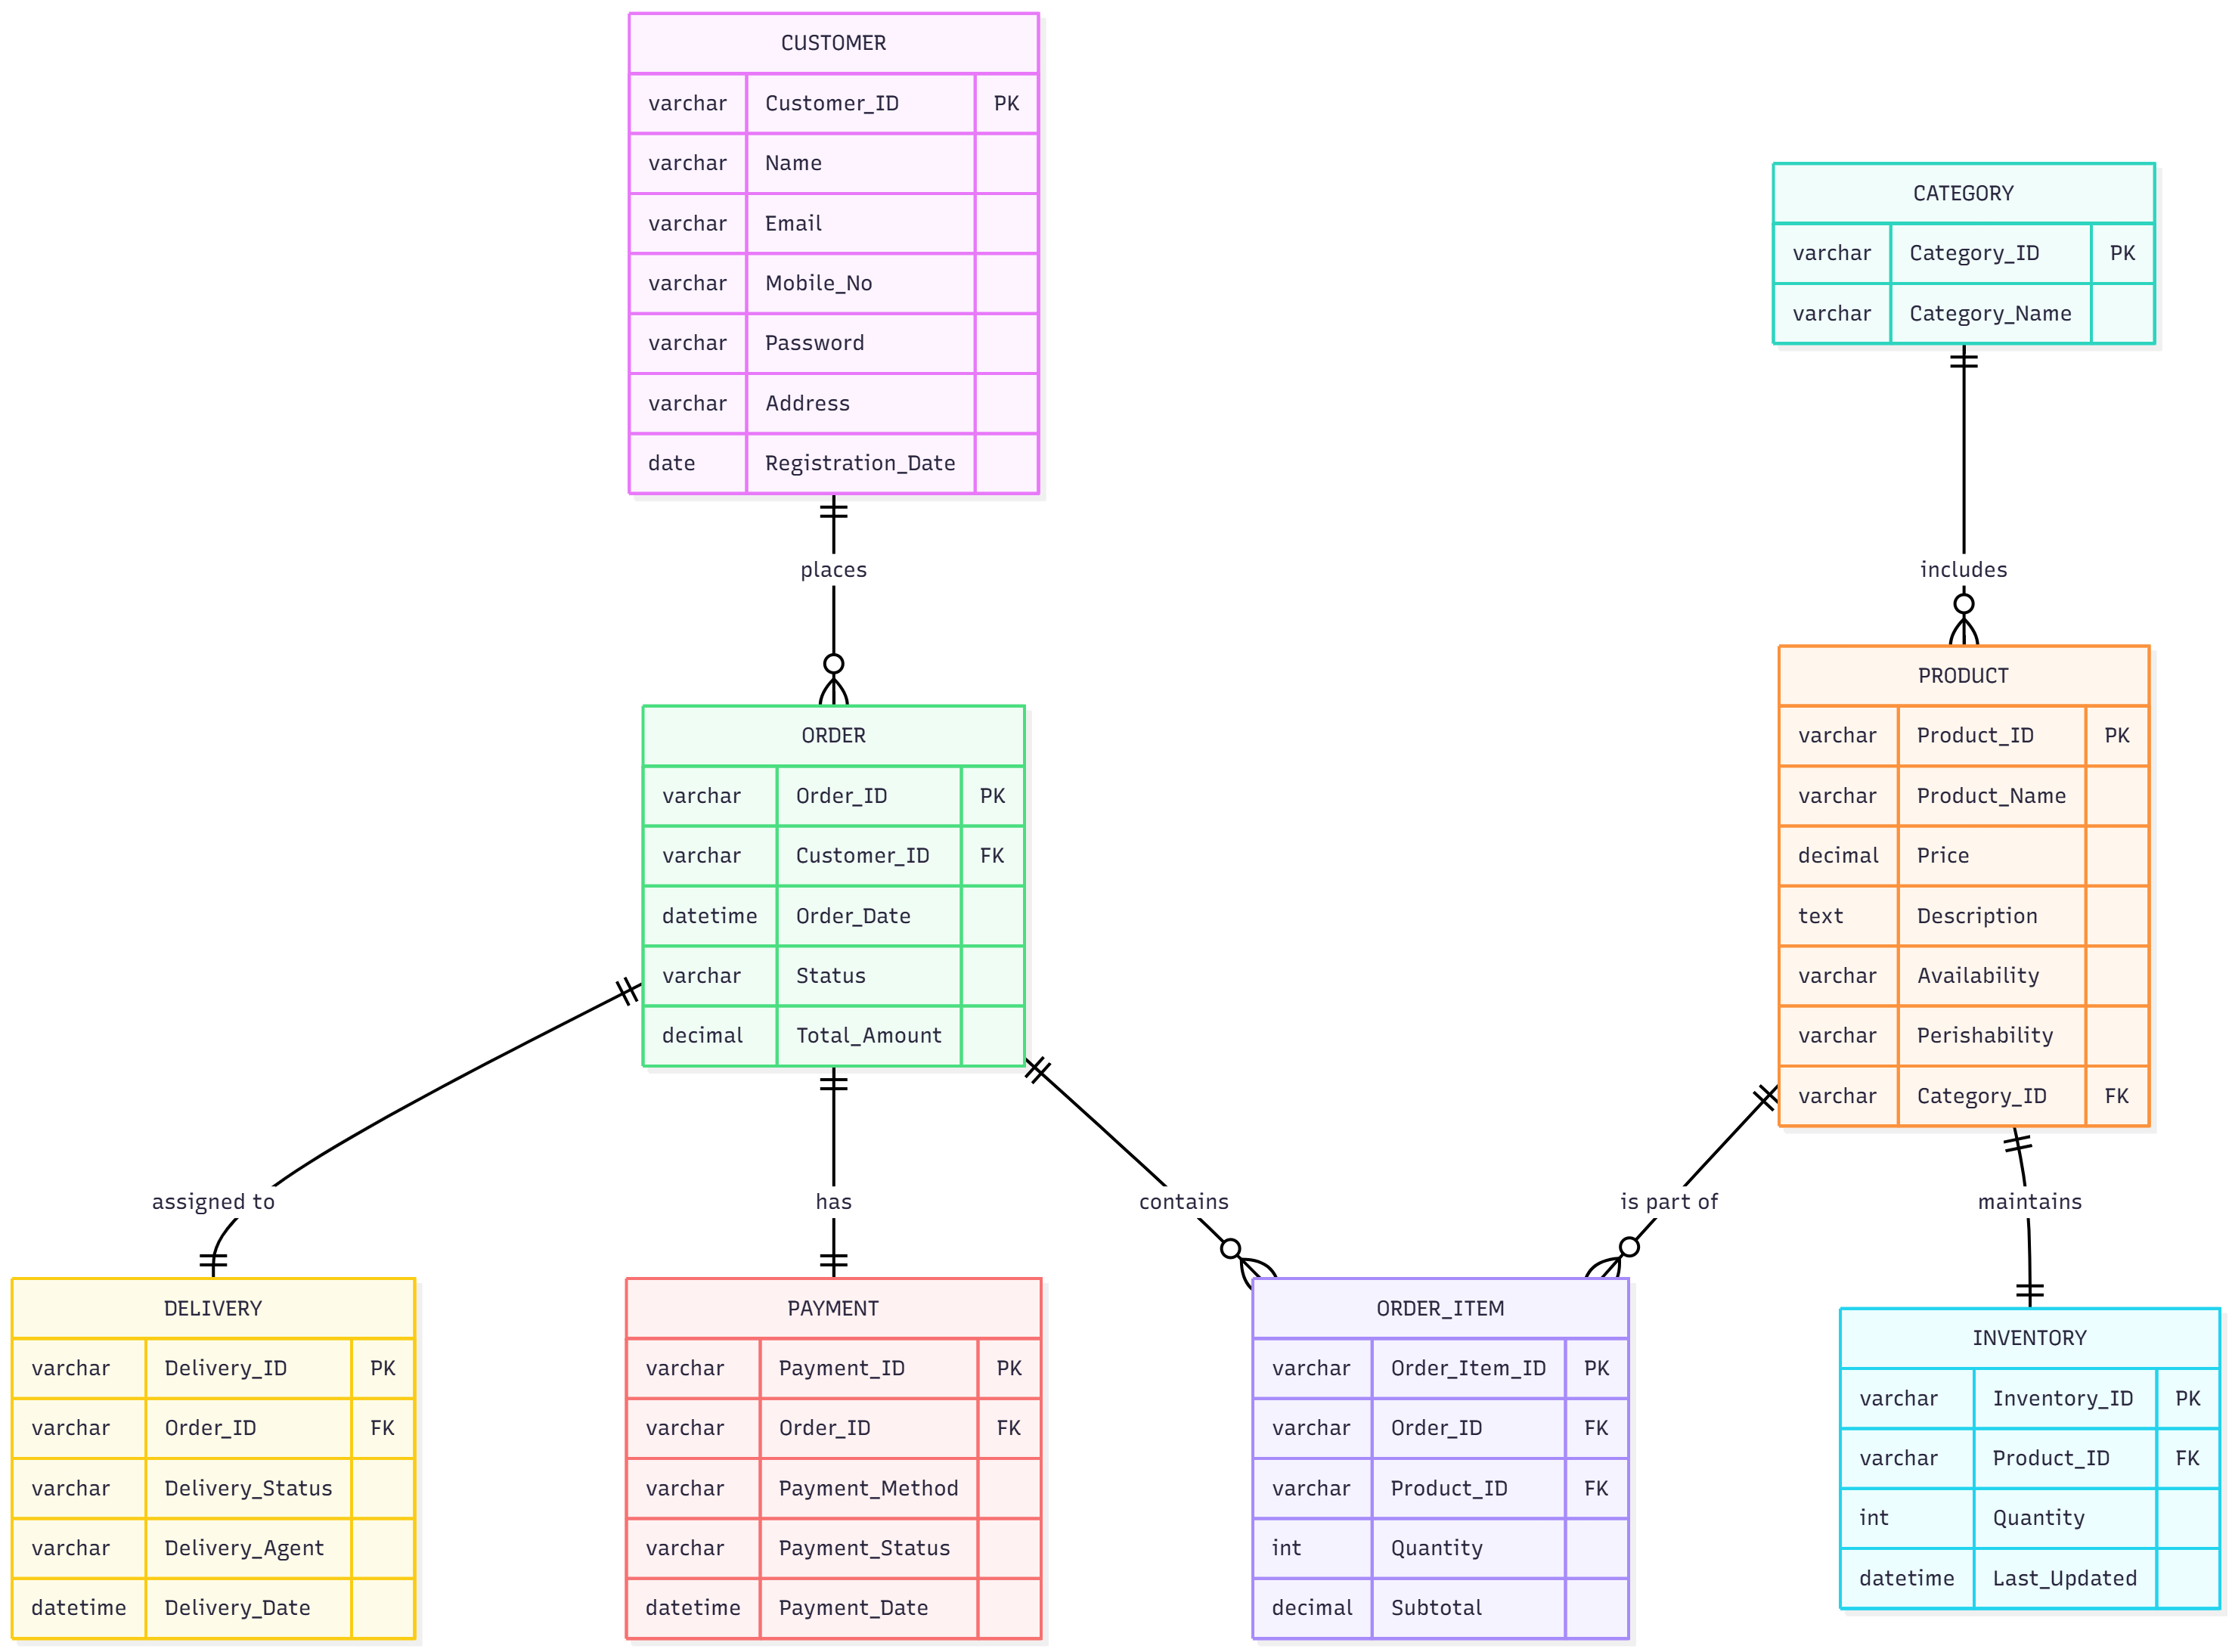
\includegraphics[width=1\textwidth]{database design/er.png} % Image not found
\caption{Entity–Relationship Diagram of Chaldal Ltd.}
\end{figure}


\subsubsection*{Entities and Their Key Attributes}

\noindent\textbf{Customer}
\begin{itemize}
    \item \textbf{Customer\_ID (PK)}
    \item Name
    \item Email
    \item Mobile\_No
    \item Address
    \item Password
    \item Registration\_Date
\end{itemize}

\noindent\textbf{Category}
\begin{itemize}
    \item \textbf{Category\_ID (PK)}
    \item Category\_Name
\end{itemize}

\noindent\textbf{Product}
\begin{itemize}
    \item \textbf{Product\_ID (PK)}
    \item Product\_Name
    \item Price
    \item Description
    \item Perishability
    \item Availability
    \item \textbf{Category\_ID (FK)}
\end{itemize}

\noindent\textbf{Inventory}
\begin{itemize}
    \item \textbf{Inventory\_ID (PK)}
    \item \textbf{Product\_ID (FK)}
    \item Quantity
    \item Last\_Updated
\end{itemize}

\noindent\textbf{Order}
\begin{itemize}
    \item \textbf{Order\_ID (PK)}
    \item \textbf{Customer\_ID (FK)}
    \item Order\_Date
    \item Status
    \item Total\_Amount
\end{itemize}

\noindent\textbf{Order\_Item}
\begin{itemize}
    \item \textbf{Order\_Item\_ID (PK)}
    \item \textbf{Order\_ID (FK)}
    \item \textbf{Product\_ID (FK)}
    \item Quantity
    \item Subtotal
\end{itemize}

\noindent\textbf{Payment}
\begin{itemize}
    \item \textbf{Payment\_ID (PK)}
    \item \textbf{Order\_ID (FK)}
    \item Payment\_Method
    \item Payment\_Status
    \item Payment\_Date
\end{itemize}

\noindent\textbf{Delivery}
\begin{itemize}
    \item \textbf{Delivery\_ID (PK)}
    \item \textbf{Order\_ID (FK)}
    \item Delivery\_Status
    \item Delivery\_Agent
    \item Delivery\_Date
\end{itemize}

\subsubsection*{Relationships Among Entities}

\begin{table}[H]
\centering
\begin{tabular}{|l|p{8cm}|c|}
\hline
\textbf{Relationship} & \textbf{Description} & \textbf{Type} \\
\hline
Customer $\rightarrow$ Order & A customer can have multiple orders, but each order belongs to one customer. & 1-to-Many \\
\hline
Category $\rightarrow$ Product & Each category can include multiple products. & 1-to-Many \\
\hline
Product $\rightarrow$ Inventory & Each product has one inventory record. & 1-to-1 \\
\hline
Order $\rightarrow$ Order\_Item & Each order can contain multiple products. & 1-to-Many \\
\hline
Product $\rightarrow$ Order\_Item & A product can appear in many orders. & 1-to-Many \\
\hline
Order $\rightarrow$ Payment & Each order has one payment transaction associated with it. & 1-to-1 \\
\hline
Order $\rightarrow$ Delivery & Each order has one delivery record. & 1-to-1 \\
\hline
\end{tabular}
\caption{Relationships Among Entities in Chaldal Ltd. Database}
\end{table}

\begin{figure}[H]
\centering
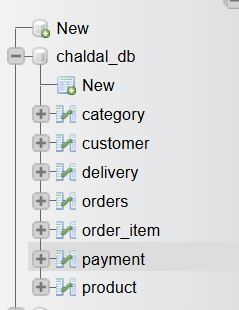
\includegraphics[width =0.5\textwidth]{database design/dbms.png} % Image not found
\caption{Database of Chaldal}
\end{figure}

\subsubsection*{Text-Based Diagram Structure (Simplified Layout)}

%% Text-based representation of the ERD %%


\subsubsection*{Description of Entity Relationships}
\begin{itemize}
    \item \textbf{Customer–Order Relationship:} Each customer can place multiple orders, while each order must belong to one registered customer.
    \item \textbf{Order–Order\_Item Relationship:} Each order can contain multiple order items; each item represents a specific product purchased within that order.
    \item \textbf{Order\_Item–Product Relationship:} Each order item corresponds to one product, defining which product is included in the order and at what quantity.
    \item \textbf{Product–Category Relationship:} Products are classified under categories such as \textit{Fruits, Vegetables, Baby Care, Staples}, etc., streamlining product organization and filtering.
    \item \textbf{Product–Inventory Relationship:} Each product maintains an inventory record that tracks its availability, quantity, and update timestamp.
    \item \textbf{Order–Payment Relationship:} Each order has a corresponding payment record that includes method (e.g., cash, card, mobile payment) and status (e.g., pending, paid).
    \item \textbf{Order–Delivery Relationship:} Each order is associated with one delivery transaction that records the delivery status, assigned agent, and completion date.
\end{itemize}

\subsubsection*{Visual Representation Guide (Simplified ER Layout)}
% \centering
%% TikZ diagram of the ERD %%

\begin{figure}[H]
\centering
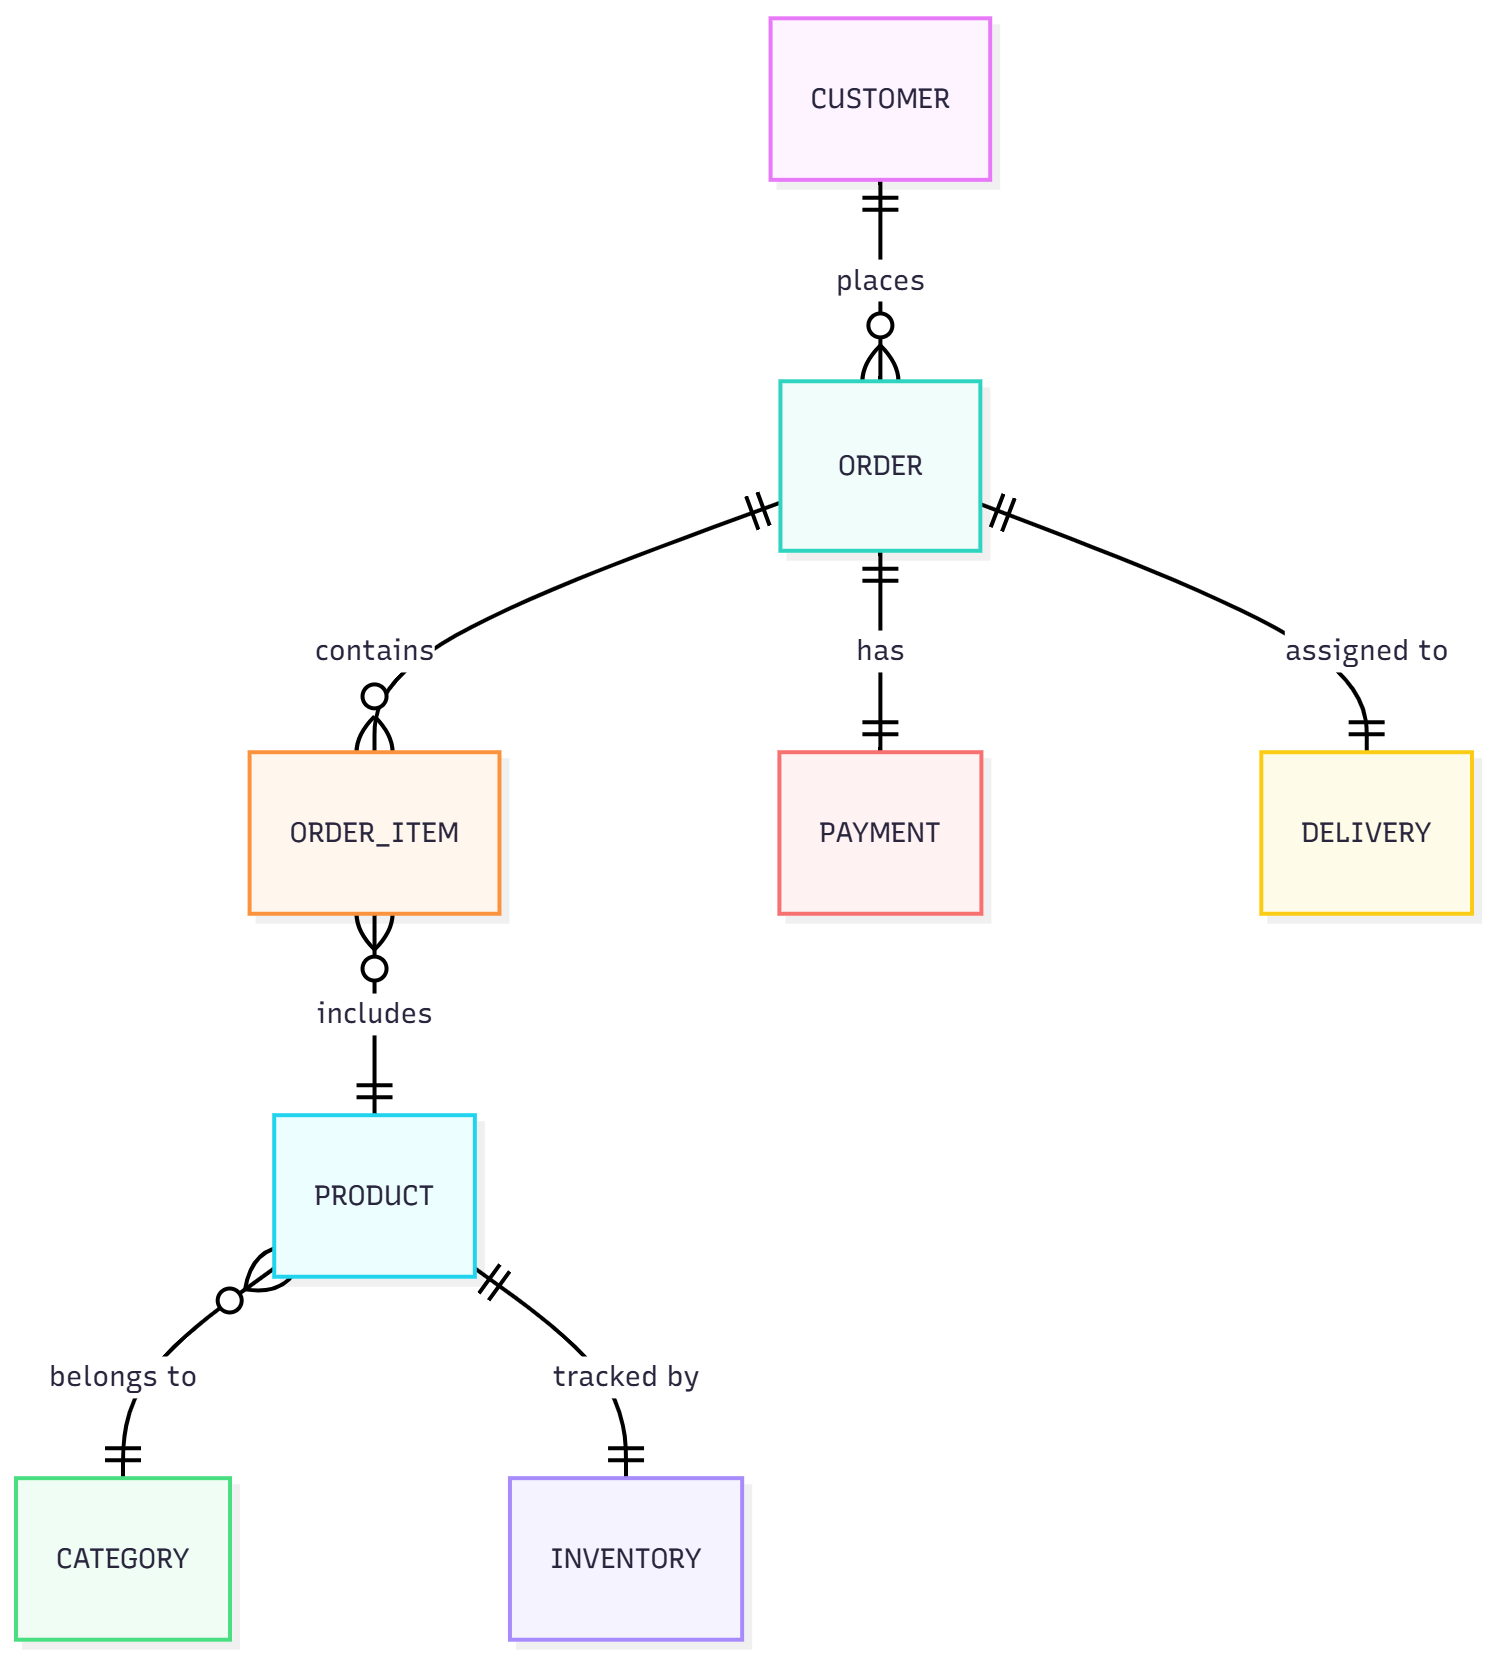
\includegraphics[width=0.6\textwidth]{database design/ers.png} % Image not found
\caption{Entity–Relationship Diagram of Chaldal Ltd.}
\end{figure}

\subsubsection{Database Table Design}

\subsubsection*{4.3.3.1 Customer Table}

\begin{table}[H]
\centering
\begin{tabular}{|l|l|l|l|p{6cm}|}
\hline
\textbf{Field Name} & \textbf{Key Type} & \textbf{Data Type} & \textbf{Size} & \textbf{Description} \\ \hline
Customer\_ID & Primary Key & VARCHAR & 10 & Unique identifier for each customer \\ \hline
Name &  & VARCHAR & 50 & Full name of the customer \\ \hline
Email &  & VARCHAR & 50 & Customer’s email address \\ \hline
Mobile\_No &  & VARCHAR & 15 & Contact number of the customer \\ \hline
Password &  & VARCHAR & 255 & Encrypted customer password \\ \hline
Address &  & VARCHAR & 255 & Physical or delivery address \\ \hline
Registration\_Date &  & DATE & --- & Date when the customer registered \\ \hline
\end{tabular}
\caption{Customer Table Design}
\end{table}

\begin{figure}[H]
\centering
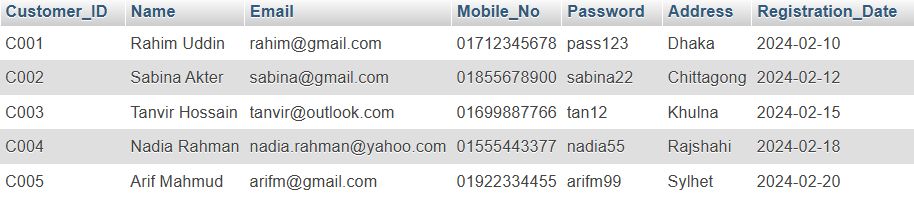
\includegraphics[width = 1\textwidth]{database design/customer.png} % Image not found
\caption{Customer Table}
\end{figure}

%------------------------------------------------

\subsubsection*{4.3.3.2 Category Table}

\begin{table}[H]
\centering
\begin{tabular}{|l|l|l|l|p{6cm}|}
\hline
\textbf{Field Name} & \textbf{Key Type} & \textbf{Data Type} & \textbf{Size} & \textbf{Description} \\ \hline
Category\_ID & Primary Key & VARCHAR & 10 & Unique ID for each category \\ \hline
Category\_Name &  & VARCHAR & 50 & Product category name (e.g., Fruits, Dairy, Household) \\ \hline
\end{tabular}
\caption{Category Table Design}
\end{table}

\begin{figure}[H]
\centering
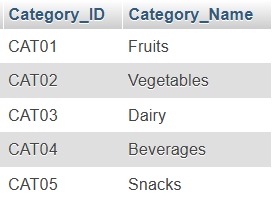
\includegraphics[width =0.4\textwidth]{database design/catagory.png} % Image not found
\caption{Category Table}
\end{figure}

%------------------------------------------------

\subsubsection*{4.3.3.3 Product Table}

\begin{table}[H]
\centering
\begin{tabular}{|l|l|l|l|p{6cm}|}
\hline
\textbf{Field Name} & \textbf{Key Type} & \textbf{Data Type} & \textbf{Size} & \textbf{Description} \\ \hline
Product\_ID & Primary Key & VARCHAR & 10 & Unique product identifier \\ \hline
Product\_Name &  & VARCHAR & 100 & Name of the product \\ \hline
Price &  & DECIMAL & (10,2) & Price of the product \\ \hline
Description &  & TEXT & --- & Product description/details \\ \hline
Availability &  & VARCHAR & 5 & Product stock status (“Yes/No”) \\ \hline
Perishability &  & VARCHAR & 5 & Product perishability (“Yes/No”) \\ \hline
Category\_ID & Foreign Key & VARCHAR & 10 & Linked to Category Table \\ \hline
\end{tabular}
\caption{Product Table Design}
\end{table}

\begin{figure}[H]
\centering
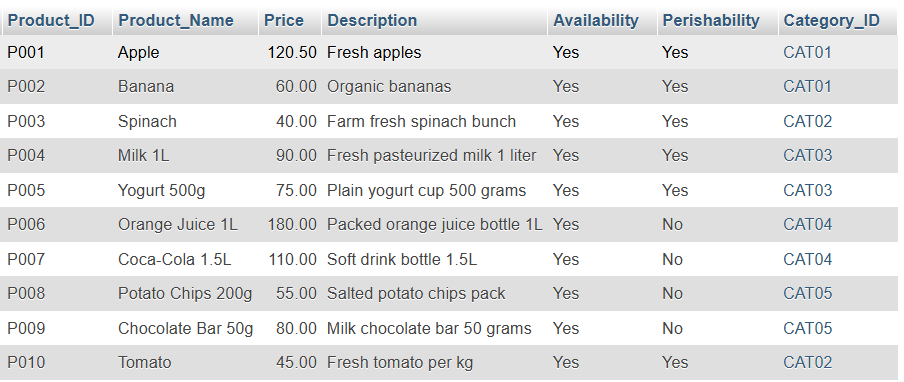
\includegraphics[width =1\textwidth]{database design/product.png} % Image not found
\caption{Prodect Table}
\end{figure}



%------------------------------------------------

\subsubsection*{4.3.3.4 Order Table}

\begin{table}[H]
\centering
\begin{tabular}{|l|l|l|l|p{6cm}|}
\hline
\textbf{Field Name} & \textbf{Key Type} & \textbf{Data Type} & \textbf{Size} & \textbf{Description} \\ \hline
Order\_ID & Primary Key & VARCHAR & 10 & Unique order identifier \\ \hline
Customer\_ID & Foreign Key & VARCHAR & 10 & Linked to Customer Table \\ \hline
Order\_Date &  & DATETIME & --- & Date and time of order placement \\ \hline
Status &  & VARCHAR & 20 & Order status (“Pending”, “Delivered”, “Cancelled”, etc.) \\ \hline
Total\_Amount &  & DECIMAL & (10,2) & Total cost of the order \\ \hline
\end{tabular}
\caption{Order Table Design}
\end{table}

\begin{figure}[H]
\centering
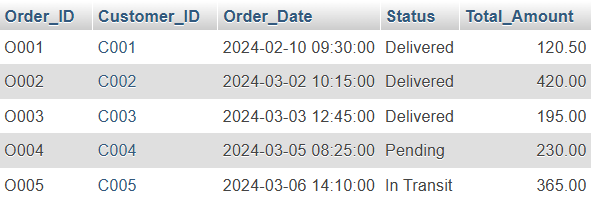
\includegraphics[width =1\textwidth]{database design/order.png} % Image not found
\caption{Order Table}
\end{figure}

%------------------------------------------------

\subsubsection*{4.3.3.5 Order\_Item Table}

\begin{table}[H]
\centering
\begin{tabular}{|l|l|l|l|p{6cm}|}
\hline
\textbf{Field Name} & \textbf{Key Type} & \textbf{Data Type} & \textbf{Size} & \textbf{Description} \\ \hline
Order\_Item\_ID & Primary Key & VARCHAR & 10 & Unique identifier for each order item \\ \hline
Order\_ID & Foreign Key & VARCHAR & 10 & Linked to Order Table \\ \hline
Product\_ID & Foreign Key & VARCHAR & 10 & Linked to Product Table \\ \hline
Quantity &  & INT & 11 & Number of product units ordered \\ \hline
Subtotal &  & DECIMAL & (10,2) & Total price for the item (Quantity × Price) \\ \hline
\end{tabular}
\caption{Order\_Item Table Design}
\end{table}
\begin{figure}[H]
\centering
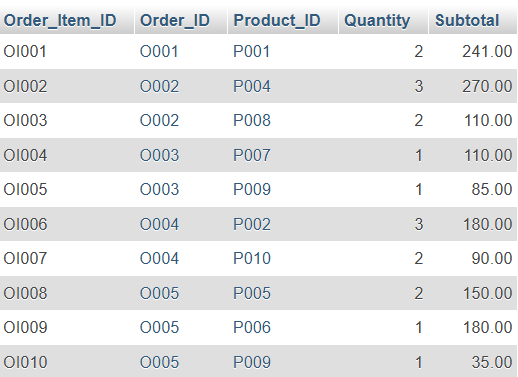
\includegraphics[width =.6\textwidth]{database design/order_item.png} % Image not found
\caption{Order Item Table}
\end{figure}
%------------------------------------------------

\subsubsection*{4.3.3.6 Payment Table}

\begin{table}[H]
\centering
\begin{tabular}{|l|l|l|l|p{6cm}|}
\hline
\textbf{Field Name} & \textbf{Key Type} & \textbf{Data Type} & \textbf{Size} & \textbf{Description} \\ \hline
Payment\_ID & Primary Key & VARCHAR & 10 & Unique identifier for payment transaction \\ \hline
Order\_ID & Foreign Key & VARCHAR & 10 & Linked to Order Table \\ \hline
Payment\_Method &  & VARCHAR & 20 & Method of payment (“Cash”, “Card”, “Mobile Payment”) \\ \hline
Payment\_Status &  & VARCHAR & 20 & Status of payment (“Pending”, “Paid”, “Failed”) \\ \hline
Payment\_Date &  & DATETIME & --- & Date and time of transaction \\ \hline
\end{tabular}
\caption{Payment Table Design}
\end{table}

\begin{figure}[H]
\centering
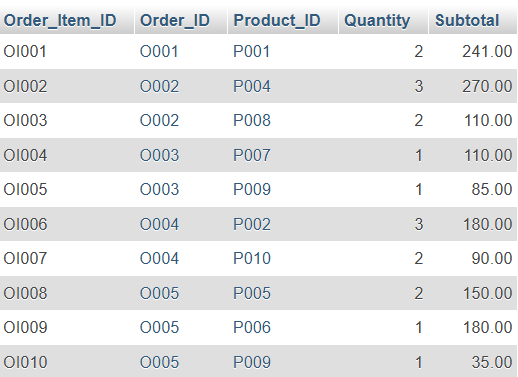
\includegraphics[width =.6\textwidth]{database design/payment.png} % Image not found
\caption{Payment Table}
\end{figure}

%------------------------------------------------

\subsubsection*{4.3.3.7 Delivery Table}

\begin{table}[H]
\centering
\begin{tabular}{|l|l|l|l|p{6cm}|}
\hline
\textbf{Field Name} & \textbf{Key Type} & \textbf{Data Type} & \textbf{Size} & \textbf{Description} \\ \hline
Delivery\_ID & Primary Key & VARCHAR & 10 & Unique identifier for each delivery \\ \hline
Order\_ID & Foreign Key & VARCHAR & 10 & Linked to Order Table \\ \hline
Delivery\_Status &  & VARCHAR & 20 & Status of the delivery (“Out for Delivery”, “Delivered”) \\ \hline
Delivery\_Agent &  & VARCHAR & 50 & Name of assigned delivery personnel \\ \hline
Delivery\_Date &  & DATETIME & --- & Date and time of successful delivery \\ \hline
\end{tabular}
\caption{Delivery Table Design}
\end{table}

\begin{figure}[H]
\centering
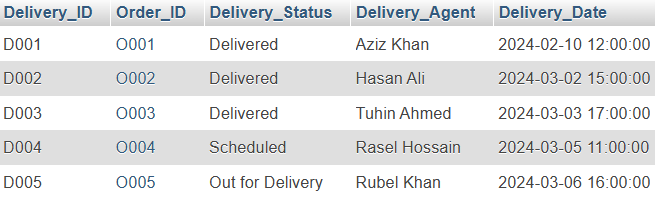
\includegraphics[width =1\textwidth]{database design/deliver.png} % Image not found
\caption{Delivery Table}
\end{figure}

%------------------------------------------------


\textbf{Notes:}
\begin{itemize}
    \item All primary keys are defined as \textbf{VARCHAR(10)} for consistency and scalability.
    \item Foreign key constraints ensure \textbf{referential integrity} across dependent tables.
    \item \textbf{DECIMAL(10,2)} is used for monetary values to maintain precision.
    \item \textbf{VARCHAR} types are chosen for alphanumeric fields such as IDs, names, and categorical data.
    \item \textbf{DATETIME} fields record important time-based events like order placement and delivery completion.
\end{itemize}

\subsection{Form Design}

Form design is a critical component of the system architecture, serving as the primary touchpoint between the user and the system's core logic. For a high-traffic e-commerce platform like Chaldal, forms must minimize cognitive load, ensure data integrity, and facilitate the system's key performance objectives, such as securing transactions (via advance payment) and gathering performance data.

This chapter details the design blueprint for the key user interface forms within the new Chaldal system. In a dynamic e-commerce environment, a poorly designed form directly translates to cart abandonment. Therefore, these designs are engineered not just for aesthetics, but as functional data collection tools that systematically address the challenges identified in the analysis phase. Specifically, these forms integrate mandatory SMS verification to combat fraudulent orders, enforce advance payment to secure revenue, utilize geo-optimized inputs for accurate delivery routing, and incorporate post-transaction feedback loops to drive continuous service improvement. By focusing on clarity, security, and integration with the logistics engine, these forms are designed to enhance user trust, accelerate the checkout process, and directly support the functionalities of the proposed Candidate System I.

\subsubsection{Secure Authentication and Account Flow}

This flow prioritizes mobile number authentication (Process 6) to prevent fraudulent accounts while maintaining social login options for user convenience, reflecting the mobile-first nature of the user base.

\begin{table}[H]
\centering
\small
\begin{tabular}{|L{3cm}|L{3.5cm}|L{7.5cm}|}
\hline
\rowcolor{tableheader!30}
\textbf{Form Component} & \textbf{Design Objective} & \textbf{Key Features \& Rationale} \\
\hline
\textbf{Primary Login/Signup} & Simplicity and Security & \textbf{Mobile Number First:} The primary screen prompts for the mobile number, followed immediately by a server-generated \textbf{One-Time Password (OTP) via SMS (Process 6)}. This replaces the vulnerable password-based sign-up. Secondary options like \textbf{Facebook Login} and \textbf{Login with Email} are provided for convenience. \\
\hline
\textbf{Profile Setup} & Data Management \& Incentive & \textbf{Fields:} Name, Phone Number, Email Address, Gender, and Date of Birth. This validates contact points and gathers demographic data for enhanced service personalization and reporting. \\
\hline
\textbf{Error Handling \& Recovery} & User Trust & \textbf{Forgot Password Flow:} A separate modal requires the Email Address to send a password reset link. This is protected by \textbf{reCAPTCHA} to prevent automated attacks. \\
\hline
\end{tabular}
\caption{Secure Authentication Components}
\label{tab:auth_components}
\end{table}

\paragraph{Login/Signup:}
The authentication module prioritizes a seamless user journey while integrating robust security measures. Registration requires standard user details and activates SMS verification (OTP) to secure accounts against fraudulent activity. The system supports multiple access points for returning users (registered email or phone number). Account maintenance is supported by a dedicated password recovery function.

\paragraph{Profile Setup:}
This form displays a profile setup page for an online service. The user can see their name, which is curiously displayed as a phone number, and their phone number itself, which appears to be pre-filled and uneditable. The page prompts the user to verify their email address in exchange for a free delivery, highlighting a key incentive. Below this, there are fields to select gender and enter a date of birth in YYYY-MM-DD format. The final section, an ``Address Book,'' indicates that the user can add or manage their delivery addresses, with a clear button to add a ``New Address.'' Overall, the page is designed to collect and manage essential user information for an account, likely for an e-commerce or delivery-based platform.
\begin{figure}[H]
    \centering
    \begin{minipage}{0.35\textwidth}
        \centering
        
\includegraphics[width=\textwidth]{login with email.png}
        \caption*{Login Screen}
    \end{minipage}
    \hfill
    \begin{minipage}{0.35\textwidth}
        \centering
        
\includegraphics[width=\textwidth]{Login with mobile.png}
        \caption*{Signup Screen}
    \end{minipage}
    \caption{Login and Signup Interface}
    \label{fig:login_signup}
\end{figure}

\begin{figure}[H]
    \centering
    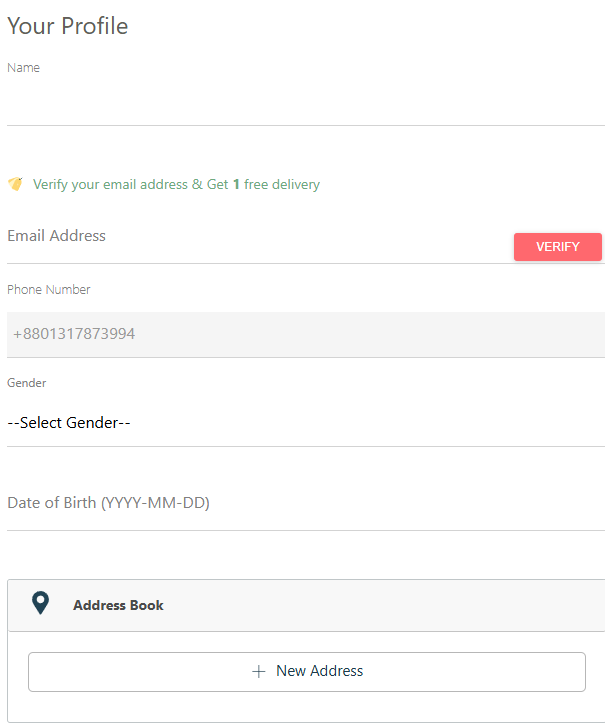
\includegraphics[width=0.6\textwidth]{Profile setup.png}
    \caption{Profile Setup Interface}
    \label{fig:profile_setup}
\end{figure}

\paragraph{Error Handling \& Recovery:}
This form shows a ``Forgot Password'' pop-up window. It has a single field for the user to enter their email address. Below the input field is a prominent red ``SUBMIT'' button. The window informs the user that they will receive a link to reset their password and notes that the site is protected by reCAPTCHA, with links to the Google Privacy Policy and Terms of Service.

\begin{figure}[H]
    \centering
    
\includegraphics[width=0.5\textwidth]{forget password.png}
    \caption{Password Recovery Modal}
    \label{fig:password_recovery}
\end{figure}

\subsubsection{Geo-Optimized Address Management and Delivery Scheduling}

This section combines personal address management (Profile/Address Book) with the required time slot selection, crucial for logistics optimization (Problem 05).

\begin{table}[H]
\centering
\small
\begin{tabular}{|L{3cm}|L{3.5cm}|L{7.5cm}|}
\hline
\rowcolor{tableheader!30}
\textbf{Form Component} & \textbf{Design Objective} & \textbf{Key Features \& Rationale} \\
\hline
\textbf{Address Book Interface} & Quick Selection & The interface displays existing addresses and includes a clear \textbf{``New Address''} button. Users can \textbf{Select a Delivery Address} from their saved locations at the start of checkout. \\
\hline
\textbf{Location Capture (Primary)} & Precision for Route Optimization & \textbf{Map Integration:} The foundational method for adding a new address must involve dropping a pin on a live map to capture precise \textbf{latitude/longitude data}. Textual inputs (Apartment/Flat Number, Landmark) serve as secondary confirmation for the delivery agent. \\
\hline
\textbf{Delivery Scheduling} & Logistics Alignment & \textbf{Preferred Delivery Time:} This dynamically displays available 30-minute \textbf{time slots}, ensuring the customer's request aligns with the current capacity of the delivery fleet and micro-warehouse to prevent order delivery disruptions. \\
\hline
\end{tabular}
\caption{Address Management and Delivery Scheduling Components}
\label{tab:address_components}
\end{table}

\begin{figure}[H]
    \centering
    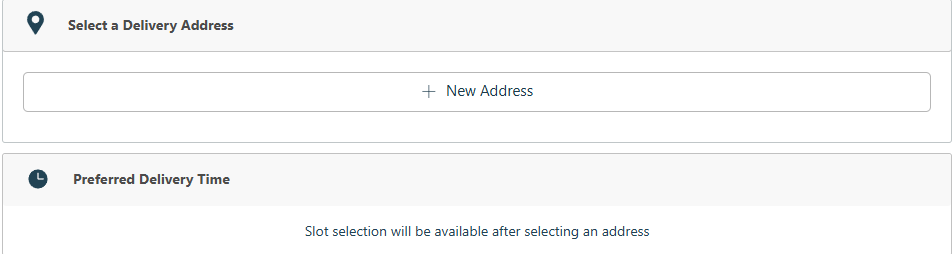
\includegraphics[width=\textwidth]{Delivery address.png}
    \caption{Address Booking and Delivery Scheduling}
    \label{fig:address_delivery}
\end{figure}

\subsubsection{Dynamic Advanced Checkout Form}

This form is the central interface for completing the transaction and directly supports the \textbf{Advance Payment} feature introduced in the system design.

\begin{table}[H]
\centering
\small
\begin{tabular}{|L{3cm}|L{3.5cm}|L{7.5cm}|}
\hline
\rowcolor{tableheader!30}
\textbf{Form Component} & \textbf{Design Objective} & \textbf{Key Features \& Rationale} \\
\hline
\textbf{Product Review (Read-Only)} & Final Order Accuracy & A scrollable, read-only list of all items, quantities, and individual prices. This prevents late-stage order edits and ensures accuracy (\textbf{Process 9.2: Verify Product List}). \\
\hline
\textbf{Payment Method} & Security and Fraud Prevention & \textbf{Advance Payment (Mandatory):} The primary option defaults to digital payment methods (Card, \textbf{bKash}, Mobile Banking). A clear note explains that \textbf{advance payment is required to reduce order fraud, aligning with Candidate System I (Process 4)}. \textit{Cash on Delivery is minimized or restricted.} \\
\hline
\textbf{Order Summary Panel} & Transparency and Trust & \textbf{Real-Time Calculation:} A persistent panel showing Subtotal, Delivery Fee (BDT 19), Applied Discounts (Flash Sales/Process 1.2), and \textbf{Total Payable Amount}. This addresses dynamic pricing confusion (Problem 04). \\
\hline
\textbf{Checkout Instructions} & Logistics Clarity & A dedicated text field allows users to provide specific notes for the delivery agent (e.g., gate code, knock softly). \\
\hline
\end{tabular}
\caption{Dynamic Advanced Checkout Form Components}
\label{tab:checkout_components}
\end{table}

\begin{figure}[H]
    \centering
    \begin{minipage}{0.45\textwidth}
        \centering
        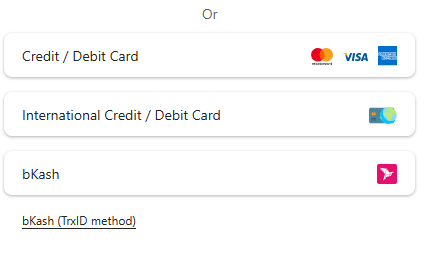
\includegraphics[width=\textwidth]{Payment method.png}
        \caption*{Payment Method Selection}
    \end{minipage}
    \hfill
    \begin{minipage}{0.45\textwidth}
        \centering
        
\includegraphics[width=\textwidth]{Instruction.png}
        \caption*{Order Summary Panel}
    \end{minipage}
    \caption{Checkout Interface Components}
    \label{fig:checkout_components}
\end{figure}

\begin{figure}[H]
    \centering
    
\includegraphics[width=\textwidth]{payment mode.png}
    \caption{Dynamic Advanced Checkout Form - Complete View}
    \label{fig:checkout_complete}
\end{figure}

\subsubsection{Post-Delivery Feedback Form}

To support the objective of tracking and improving delivery performance, a concise and mandatory feedback form is presented immediately after the Delivery Confirmation via a notification.

\begin{table}[H]
\centering
\small
\begin{tabular}{|L{3cm}|L{3.5cm}|L{7.5cm}|}
\hline
\rowcolor{tableheader!30}
\textbf{Form Component} & \textbf{Design Objective} & \textbf{Key Features \& Rationale} \\
\hline
\textbf{Delivery Timeliness} & Metric Tracking & \textbf{Rating Scale (1-5 Stars):} ``How timely was your delivery?'' (Measures adherence to selected slot). \\
\hline
\textbf{Product Condition} & Quality Assurance & \textbf{Binary/Short Text:} ``Were all perishable items fresh?'' (Yes/No with a small comment box). \\
\hline
\textbf{Delivery Agent Performance} & Bonus Eligibility Data & \textbf{Rating Scale (1-5 Stars):} ``How would you rate the courtesy and professionalism of the delivery staff?'' (\textbf{Directly feeds into Process 11.3: Bonus Payment}). \\
\hline
\textbf{Overall Satisfaction} & General Experience & \textbf{NPS Score (0-10):} ``How likely are you to recommend Chaldal?'' (Measures overall satisfaction and loyalty). \\
\hline
\end{tabular}
\caption{Post-Delivery Feedback Form Components}
\label{tab:feedback_components}
\end{table}

\subsubsection{Summary of Design Impact}

These form designs are not merely data entry screens but are structured instruments that drive systemic improvement and financial stability across the Chaldal ecosystem. By embedding security, efficiency, and accountability into every user interaction---from mobile authentication to mandatory advance payment and performance-linked feedback---these forms directly resolve the core operational and financial risks identified in the analysis phase. 

\paragraph{Key Benefits:}
\begin{itemize}
    \item \textbf{Data-Driven Operations:} Every customer action contributes valuable, trackable data, transforming the user interface into a powerful mechanism for logistics optimization, fraud reduction, and sustained customer loyalty.
    
    \item \textbf{Financial Stability:} Cash flow is stabilized by prioritizing digital payment methods, reducing the risks associated with cash-on-delivery transactions.
    
    \item \textbf{Operational Transparency:} Enhanced through geotagging and precise location data, enabling better route optimization and delivery planning.
    
    \item \textbf{Performance-Driven Culture:} Service quality data is linked directly to incentive structures for delivery staff, fostering accountability and excellence.
    
    \item \textbf{Strategic Transformation:} The comprehensive nature of these inputs fundamentally elevates the business from a transactional e-commerce service to a data-centric logistics platform.
\end{itemize}

\paragraph{Integration with System Processes:}
The forms are designed to seamlessly integrate with the following key processes:
\begin{itemize}
    \item \textbf{Process 6:} SMS-based OTP verification for secure authentication
    \item \textbf{Process 4:} Mandatory advance payment to reduce fraud
    \item \textbf{Process 9.2:} Product list verification before checkout
    \item \textbf{Process 1.2:} Dynamic pricing and flash sale integration
    \item \textbf{Process 11.3:} Performance-based bonus payment for delivery agents
\end{itemize}

These form designs ensure that every interaction not only serves the immediate user need but also contributes to the broader system objectives of efficiency, security, and continuous improvement.


\subsection{Conclusion}
In summary, the design phase has translated Chaldal’s strategic objectives and analytical findings into a robust, scalable, and user-centric system architecture. Through the integration of cloud-based infrastructure, digitalized supply chain and HR processes, and optimized user interfaces, the proposed design addresses all critical operational, financial, and customer experience challenges identified in earlier chapters. The new system ensures data integrity, security, and efficiency across all business domains—enabling real-time analytics, transparent workflows, and seamless user interactions.

By implementing these design solutions, Chaldal is positioned to achieve significant cost savings, improved service quality, and enhanced customer satisfaction. The modular and extensible nature of the design supports future growth, technological innovation, and rapid adaptation to evolving market demands. Ultimately, this comprehensive design lays the foundation for Chaldal’s transformation into a data-driven, operationally excellent, and financially sustainable leader in Bangladesh’s e-commerce and logistics sector.

\end{document}